%!TEX encoding = UTF-8 Unicode
\documentclass{lecturenotes}
\usepackage[swedish]{babel}
\input{../compendium/global-constants.tex}

\setbeamertemplate{footline}[frame number]
\title[Föreläsningar EDAA45 pgk, Björn Regnell, \today]{EDAA45 Programmering, grundkurs}
\subtitle{Föreläsningar}
\author{Björn Regnell}
\institute{Datavetenskap, LTH}
\date{Kompileringsdatum: \today}

\setbeamerfont{section in toc}{size=\small}

\setbeamerfont{subsection in toc}{size=\footnotesize}

\begin{document}

%\renewcommand{\pause}{}
\input{../compendium/generated/names-generated.tex}


\newcommand{\Lecture}[2]{%
\section[Vecka #1: #2]{#2}%
\frame{\tableofcontents[currentsubsection,hideothersubsections,sections={#1}]}}

\frame{\titlepage}
\frame{
\vspace{-1.5em}\begin{multicols}{2}
\footnotesize\tableofcontents[subsectionstyle=hide,sections={1-7}]

\columnbreak

\footnotesize\tableofcontents[subsectionstyle=hide,sections={8-14}]
\end{multicols}
}

\Lecture{1}{\ModWeekONE}
\input{body/lect-w01-about.tex}
\input{body/lect-w01-intro.tex}

\Lecture{2}{\ModWeekTWO}
\input{body/lect-w02-how-to-study.tex}
\input{body/lect-w02-codestruct.tex}

\Lecture{3}{\ModWeekTHREE}
\input{body/lect-w03-course-ombudsmen.tex}
\input{body/lect-w03-functions.tex}

\Lecture{4}{\ModWeekFOUR}
%!TEX encoding = UTF-8 Unicode
%!TEX root = ../lect-w04.tex

\ifkompendium\else
\begin{SlideExtra}{Denna vecka: Objekt}
\begin{itemize}\SlideFontSmall
\item Övning \texttt{objects} innehåller bland annat:
\begin{itemize}\SlideFontTiny
\item hur man kan kapsla in funktioner och variabler i singelobjekt
\item hur man kan skapa namnrymder, hantera namnöverskuggning, och använda punktnotation
%\item skapa objekt med hjälp av tupler
%\item lat initialisering
%\item jar-fil, paket, namnbyte vid import
\item använda färdiga klasser, t.ex. \code{java.awt.Color}
\item händelsehantering i ett grafiskt fönster
\end{itemize}

\item På laboration \texttt{blockmole} lär du dig bland annat:
\begin{itemize}\SlideFontTiny
  \item att dela upp din kod i flera singelobjekt
  \item att använda färdig klass: \code{introprog.PixelWindow}
  \item att skapa ett större program i form av ett grafiskt spel
  \item använda tidigare begrepp: uttryck, program och funktioner
\end{itemize}

\item Senaste versionen av kursbiblioteket \code{introprog} är \Emph{\LibVersion} 
\begin{itemize}\SlideFontTiny
\item Jar-fil kan laddas ned här: \url{https://fileadmin.cs.lth.se/introprog.jar}
\item Eller låt \texttt{scala-cli} ladda ner den med
\begin{Code}
//> using scala "3.1.3"
//> using lib "se.lth.cs::introprog:1.3.1"  
\end{Code} 
\item Se \Emph{dokumentation} här: \url{http://cs.lth.se/pgk/api}
\end{itemize}
\end{itemize}
\end{SlideExtra}
\fi


\Subsection{Vad är ett objekt?}

\ifkompendium\else
\begin{SlideExtra}{Objekt är ungefär som äggkartonger}
  \begin{tabular}{l r}
    \includegraphics[width=0.5\textwidth]{../img/egg-box}
    &
    \includegraphics[width=0.5\textwidth]{../img/egg-box-closed}
  \end{tabular}
  Men de kan innehålla mer än bara ägg...
\end{SlideExtra}
\fi

\begin{Slide}{Vad rymmer sköldpaddan i Kojo i sitt tillstånd?}
\centering
\includegraphics[width=0.7\textwidth]{../img/kojo}

\pause position, riktning, färg, bredd, penna uppe/nere, fyll-färg
\end{Slide}



\begin{Slide}{Vad är ett objekt?}
\begin{itemize}
\item Ett objekt är en abstraktion som...
\begin{itemize}
  \item kan innehålla \Emph{data} som objektet ''håller reda på'' och
  \item kan erbjuda \Emph{operationer} som \emph{gör} något eller ger ett \emph{värde}
\end{itemize}

\pause

\item Exempel: Sköldpaddan i Kojo \includegraphics[width=0.08\textwidth]{../img/turtle.png}
\begin{itemize}
  \item Vilken \Emph{data} sparas av sköldpaddan?
  \pause
  \item[] position, rikting, pennfärg, ...

  \item Vilka \Emph{operationer} kan man be sköldpaddan att utföra?

  \item[] fram, höger, vänster, ...
  \pause


\end{itemize}

\item Terminologi:
\begin{itemize}
  \item objektets data sparas i variabler som kallas \Alert{attribut}
  \item alla variabelvärden utgör tillsammans objektets \Alert{tillstånd}
  \item operationerna är funktioner i objektet och kallas \Alert{metoder}
  \item attribut, metoder (och annat i objektet) kallas \Alert{medlemmar}
\end{itemize}
\end{itemize}
\end{Slide}



\begin{Slide}{Deklarera, allokera, referera}
Olika saker man kan göra med objekt:
\begin{itemize}
  \item \Emph{deklarera}: att skriva kod som beskriver objekt; \\
  finns flera sätt: singelobjekt, klass, tupel, ...
  \item \Emph{allokera}: att skapa plats i minnet för objektet vid körtid
  \item \Emph{referera}: att använda objektet via ett namn;\\
  man kommer åt innehållet i ett objekt med \Alert{punktnotation}: \\
  \code{ref.medlem}
  \pause
  \item (\Emph{avallokera}): att frigöra minne för objekt som inte längre används;
  detta \Alert{sker automatiskt} i Scala, men i många andra språk,
  t.ex. C++, får man själv hålla reda på avallokering,
  vilket är knepigt och det blir lätt svåra buggar.
\end{itemize}
\end{Slide}


\begin{Slide}{Olika sätt att allokera objekt}\SlideFontSmall
\begin{enumerate}

\item Använda en \Emph{färdig funktion} som skapar ett objekt åt oss, t.ex. \code{apply}:
\begin{Code}
Vector(1,2,3)  // skapa Vector-objekt med apply-metod
Vector.apply(1,2,3)  // explicit apply
\end{Code}
{\SlideFontTiny En funktion som skapar objekt kallas \Alert{fabriksmetod} \Eng{factory method}.\vspace{0.5em}}

\item Göra \code{new} på en klass (mer om klasser senare):
\begin{Code}
new introprog.PixelWindow() // skapa ett fönsterobjekt
\end{Code}
{
\SlideFontSmall Med \code{new} kan man skapa \Alert{många upplagor} av samma typ av objekt.\\
I Scala 3 kan \code{new} ofta utelämnas: \code{introprog.PixelWindow()}
}

\item Deklarera ett \Emph{singelobjekt} med nyckelordet \code{object}
\begin{itemize}\SlideFontSmall
  \item Ett singelobjekt finns i exakt \Alert{en} upplaga.
  \item Allokeras \Alert{automatiskt} första gången man refererar objektet; \\
  man behöver inte, och kan inte, skriva \code{new}.
  \pause
  \item Medlemmar i ett Scala-singelobjekt liknar \jcode{static}-medlemmar i en Java/C++/C\#-klass.
\end{itemize}
\item Använda en \Emph{tupel}, exempel: \code{val p = (200, 300)}
\end{enumerate}
\end{Slide}

\Subsection{Singelobjekt}

\begin{Slide}{Vad är ett singelobjekt?}
\begin{itemize}\SlideFontSmall
\item Ett singelobjekt \Eng{singelton} deklareras med nyckelordet \code{object} och används för att samla \Emph{medlemmar} \Eng{members} som \Alert{hör ihop}.
\item Ett singelobjekt kallas också \Emph{modul} \Eng{module}.
\item Medlemmarna kan t.ex. vara \Emph{variabler} (\code{val}, \code{var}) och \Emph{metoder} (\code{def}). 
\item En \Alert{metod} är en \Emph{funktion} som finns i ett objekt. Metoder kallas även \Emph{operationer}.
\item Exempel: singelobjekt/modul som hanterar highscore:
\begin{Code}
object Highscore {
  var highscore = 0
  def isHighscore(points: Int): Boolean = points > highscore
}
\end{Code}
\item Krullparenteser är valfria i Scala 3:\\~~~du kan använda kolon och indentering i stället.
\pause
\item Tanken är ofta att abstraktioner ska vara användbar i annan kod, för att underlätta när man bygger applikationer, och kallas då ett \Emph{API} (Application Programming Interface). Exempel: ett highscore-API.
\end{itemize}
\end{Slide}


\begin{Slide}{Allokering: minne reserveras med plats för data}
\begin{Code}
object Highscore:
  var highscore = 0
  def isHighscore(points: Int): Boolean = points > highscore

\end{Code}
\pause
\begin{tikzpicture}[font=\large\sffamily]
\matrix [matrix of nodes, row sep=0, column 2/.style={nodes={rectangle,draw,minimum width=0.8cm}}] (mat)
{
\texttt{Highscore}   &  \makebox(10,10){ }\\
%\texttt{g2}   &  \makebox(16,12){ }\\
};
\node[cloud, cloud puffs=13.0, cloud ignores aspect, minimum width=2cm, minimum height=3.8cm,
 align=center, draw] (x) at (5.8cm, -1.5cm) {
 \begin{tabular}{r l}
 \texttt{highscore} & \fbox{~~~~~0~~} \\

 \end{tabular}
 };
\filldraw[black] (1.2cm,0.0cm) circle (3pt) node[] (ref) {};
 \draw [arrow, line width=0.7mm] (ref) -- (x);
% \node[cloud, cloud puffs=15.7, cloud ignores aspect, %minimum width=5cm, minimum height=2cm,
% align=center, draw] (g2) at (5cm, -2cm) {Gurka-\\objekt};
% \filldraw[black] (0.4cm,-0.4cm) circle (3pt) node[] (g2ref) {};
% \draw [arrow] (g2ref) -- (g2);
\end{tikzpicture}
\end{Slide}


\begin{Slide}{Punktnotation, tillståndsförändring med tilldelning}
\begin{REPLnonum}
scala> Highscore.isHighscore(5)
res0: Boolean = true

scala> Highscore.highscore = 42
\end{REPLnonum}
\pause
\begin{tikzpicture}[font=\large\sffamily]
\matrix [matrix of nodes, row sep=0, column 2/.style={nodes={rectangle,draw,minimum width=0.8cm}}] (mat)
{
\texttt{Highscore}   &  \makebox(10,10){ }\\
%\texttt{g2}   &  \makebox(16,12){ }\\
};
\node[cloud, cloud puffs=13.0, cloud ignores aspect, minimum width=2cm, minimum height=3.8cm,
 align=center, draw] (x) at (5.8cm, -1.5cm) {
 \begin{tabular}{r l}
 \texttt{highscore} & \fbox{~~~~42~~} \\

 \end{tabular}
 };
\filldraw[black] (1.2cm,0.0cm) circle (3pt) node[] (ref) {};
 \draw [arrow, line width=0.7mm] (ref) -- (x);
% \node[cloud, cloud puffs=15.7, cloud ignores aspect, %minimum width=5cm, minimum height=2cm,
% align=center, draw] (g2) at (5cm, -2cm) {Gurka-\\objekt};
% \filldraw[black] (0.4cm,-0.4cm) circle (3pt) node[] (g2ref) {};
% \draw [arrow] (g2ref) -- (g2);
\end{tikzpicture}
\end{Slide}


\begin{Slide}{Punktnotation och operatornotation}
Punktnotation där metodanropet har \Alert{ett} enda argument:\\~\\
\code{objekt.metod(argument)}
\\~\\kan även skrivas med infix \Emph{operatornotation}:\\~\\
\code{objekt metod argument}
\\~\\Exempel:\\
\code{1 + 2}\\\pause\vspace{0.5em}
\code{Highscore isHighscore 1000}
\pause 
{
\SlideFontSmall
\\\vspace{0.5em}Operatornotation med metoder vars namn börjar med bokstäver kommer i framtiden kräva deklaration med \code{infix} före \code{def}, detta för att uppmuntra konsekvent användning.
}
\end{Slide}


\begin{Slide}{Namnrymd och skuggning}
\begin{itemize}\SlideFontSmall
  \item En \Emph{namnrymd}\footnote{\url{https://sv.wikipedia.org/wiki/Namnrymd}}  \Eng{namespace} är en omgivning (kontext) i vilken alla namn är unika. Genom att skapa flera olika namnrymder
  kan man undvika ''\Alert{krockar}'' mellan lika namn med olika betydelser (homonymer). \\
  Exempel: mejladresser \code{kim@företag1.se}  ~$\neq$~  \code{kim@företag2.se}
  \item Medlemmarna i ett singelobjekt finns i en egen namnrymd,
  där alla namn måste vara unika på samma nivå. De ''krockar'' inte med namn ''utanför'' objektet. Dock kan det förekomma \Alert{skuggning} \Eng{shadowing}:
\end{itemize}
\begin{Code}
object Game {

  val highscore = 42   // ett annat värde än Game.Highscore.highscore

  object Highscore:
    var highscore = 0  // ett annat värde än Game.highscore
    def isHighscore(points: Int): Boolean = points > highscore
}
\end{Code}

\end{Slide}



\begin{Slide}{Inkapsling: att dölja interna delar}\SlideFontSmall
Med nyckelordet \code{private} döljs interna delar för omvärlden.
Privata medlemmar kan bara refereras \emph{inifrån} objektet.
Denna princip kallas \Emph{inkapsling} \Eng{encapsulation}.
\begin{CodeSmall}
object Highscore:
  private var myHighscore = 0        // namnet myHighscore syns ej utåt
  def highscore: Int = myHighscore   // en s.k. getter ger ett attributvärde
  def isHighscore(points: Int): Boolean = points > myHighscore
  def update(points: Int): Unit = if isHighscore(points) then myHighscore = points
\end{CodeSmall}
\pause
Varför har man nytta av detta?
\begin{itemize}
  \item Förhindra att man av misstag ändrar objekts tillstånd på fel sätt.
  \item Förhindra användning av kod som i framtiden kan komma att ändras.
  \item Erbjuder en enklare ''utsida'' genom dölja komplexitet ''på insidan''.
  \item Inte ''skräpa ner'' namnrymden med ''onödiga'' namn.
\end{itemize}
Nackdelar:
\begin{itemize}
  \item Begränsar användningen, har ej tillgång till alla delar.
  \item Svårare att experimentera med ett API medan man försöker förstå det.
\end{itemize}
\end{Slide}



\begin{Slide}{Idiom: Privata variabler med understreck vid ''krock''}\SlideFontSmall
\Emph{Idiom}: (d.v.s. ett typiskt, allmänt accepterat sätt att skriva kod)
\begin{itemize}
  \item Om namnet på en privat variabel krockar med namnet på en getter
  brukar man börja det privata namnet med ett understreck:
\end{itemize}

\begin{CodeSmall}
object Highscore:
  private var _highscore = 0
  def highscore: Int = _highscore
  def isHighscore(points: Int): Boolean = points > _highscore
  def update(points: Int): Unit = if isHighscore(points) then _highscore = points
\end{CodeSmall}

\pause

{\SlideFontTiny Namnkrock mellan metoder och variabler uppkommer inte i Java m.fl. språk, där dessa finns i \emph{olika} namnrymder.
Men i Scala har man valt att principen om \Emph{enhetlig access} ska gälla och alla medlemmar (både metoder och variabler) finns därmed i en gemensam namnrymd.}

\end{Slide}

\begin{Slide}{Principen om enhetlig access}\SlideFontSmall
  \begin{itemize}
    \item I Scala så ser access av attribut och anrop av metoder, som är deklarerade utan parameterlista, likadana ut. 
\begin{Code}
object A1 { val a = 42 }  
object A2 { def a = (41 + math.random()).round.toInt }
\end{Code}
\begin{REPLnonum}
scala> A1.a
scala> A2.a  
\end{REPLnonum}
    \item Många andra språk har olika syntax för access av attribut och anrop av metoder (t.ex. Java m.fl., där alla metodanrop måste ha parenteser).
    \item Fördel: Det går lätt att ändra i implementationen och växla mellan att använda attribut och använda metoder utan att den kod som använder din implementation behöver ändras.
    \item Nackdel: Det kan bli namnkrockar mellan metoder och attribut eftersom de finns i samma namnrymd.
  \end{itemize}
  
\end{Slide}



\begin{Slide}{Exempel: singelobjektet med förändringsbart tillstånd} \SlideFontSmall
\begin{Code}[basicstyle=\ttfamily\fontsize{9}{11}\selectfont]
object mittBankkonto:
  val kontonr: Long        = 1234567L
  var saldo: Int           = 1000
  def ärSkuldsatt: Boolean = saldo < 0
\end{Code}
\begin{REPLnonum}
scala> mittBankkonto.saldo -= 25000

scala> mittBankkonto.ärSkuldsatt
res0: Boolean = true
\end{REPLnonum}

(Vi ska i nästa vecka se hur man med s.k. klasser kan skapa många upplagor av samma  typ av objekt, så att vi kan ha flera olika bankkonto.)
\end{Slide}



\begin{Slide}{Exempel: tillstånd, attribut}
Ett objekts \Emph{tillstånd} är den samlade uppsättningen av värden av alla de attribut som finns i objektet.
\begin{Code}[basicstyle=\ttfamily\fontsize{9}{11}\selectfont]
object mittBankkonto
  val kontonr: Long        = 1234567L
  var saldo: Int           = 1000
  def ärSkuldsatt: Boolean = saldo < 0
\end{Code}
\begin{tikzpicture}[font=\large\sffamily]
\matrix [matrix of nodes, row sep=0, column 2/.style={nodes={rectangle,draw,minimum width=0.8cm}}] (mat)
{
\texttt{mittBankkonto}   &  \makebox(10,10){ }\\
%\texttt{g2}   &  \makebox(16,12){ }\\
};
\node[cloud, cloud puffs=13.0, cloud ignores aspect, minimum width=2cm, minimum height=3.8cm,
 align=center, draw] (x) at (5.8cm, -1.5cm) {
 \begin{tabular}{r l}
 \texttt{kontonr} & \fbox{1234567L} \\
 \texttt{saldo} & \fbox{1000}\\
 \end{tabular}
 };
\filldraw[black] (1.7cm,0.0cm) circle (3pt) node[] (ref) {};
 \draw [arrow, line width=0.7mm] (ref) -- (x);
% \node[cloud, cloud puffs=15.7, cloud ignores aspect, %minimum width=5cm, minimum height=2cm,
% align=center, draw] (g2) at (5cm, -2cm) {Gurka-\\objekt};
% \filldraw[black] (0.4cm,-0.4cm) circle (3pt) node[] (g2ref) {};
% \draw [arrow] (g2ref) -- (g2);
\end{tikzpicture}
\end{Slide}


\begin{Slide}{Tillståndsändring}

När en variabel tilldelas ett nytt värde sker en \Emph{tillståndsändring}. Ett \Emph{förändringsbart objekt} \Eng{mutable object} har ett \Emph{förändringsbart tillstånd} \Eng{mutable state}.

\begin{REPLnonum}
scala> mittBankkonto.saldo -= 25000

scala> mittBankkonto.saldo
res1: Int = -24000
\end{REPLnonum}
\begin{tikzpicture}[font=\large\sffamily]
\matrix [matrix of nodes, row sep=0, column 2/.style={nodes={rectangle,draw,minimum width=0.8cm}}] (mat)
{
\texttt{mittBankkonto}   &  \makebox(10,10){ }\\
%\texttt{g2}   &  \makebox(16,12){ }\\
};
\node[cloud, cloud puffs=13.0, cloud ignores aspect, minimum width=2cm, minimum height=3.8cm,
 align=center, draw] (x) at (5.8cm, -1.5cm) {
 \begin{tabular}{r l}
 \texttt{kontonr} & \fbox{1234567L} \\
 \texttt{saldo} & \fbox{-24000}\\
 \end{tabular}
 };
\filldraw[black] (1.7cm,0.0cm) circle (3pt) node[] (ref) {};
 \draw [arrow, line width=0.7mm] (ref) -- (x);
% \node[cloud, cloud puffs=15.7, cloud ignores aspect, %minimum width=5cm, minimum height=2cm,
% align=center, draw] (g2) at (5cm, -2cm) {Gurka-\\objekt};
% \filldraw[black] (0.4cm,-0.4cm) circle (3pt) node[] (g2ref) {};
% \draw [arrow] (g2ref) -- (g2);
\end{tikzpicture}
\end{Slide}

\Subsection{Paket}

\begin{Slide}{Modul}

  \begin{itemize}
    \item En modul samlar kod som utgör en sammanhållen, avgränsad \Emph{uppsättning abstraktioner} som kan användas av annan kod  för att lösa ett specifikt (del)problem.
    \item I Scala finns två sätt att skapa moduler:\footnote{\href{https://en.wikipedia.org/wiki/Modular_programming}{en.wikipedia.org/wiki/Modular\_programming}}
    \begin{itemize}
      \item \Emph{singelobjekt} med nyckelordet \code{object} och
      \item \Emph{paket} med nyckelordet \code{package}
      \pause
      \item Liknar varandra; t.ex. kan man använda punktnotation och göra \code{import} på medlemmar i både singelobjekt och paket.
      \pause
      \item Skillnader:
      \begin{itemize} 
        \item paket medför att \Alert{underkataloger} för maskinkoden skapas vid kompilering
        \item objekt kan ärva medlemmar från klasser och traits (mer om det senare)
        %\item paket får inte i Scala 2 innehålla variabel- och funktions- deklarationer på topp-nivå; dessa  måste i Scala 2 ligga inuti singelobjekt eller klasser
      \end{itemize}
      %\item I Scala 2 kan toppnivådekl. placeras i ett \code{package object}
    \end{itemize}
  
  \end{itemize}
\end{Slide}

\begin{Slide}{Deklarera paket}
Med nyckelordet \code{package} först i en kodfil ges alla deklarationer en gemensam namnrymd.\\
\vspace{1em}
Denna kod ligger i filen \texttt{f1.scala}:
\begin{Code}
package mittpaket

object A: 
  def hälsa: Unit = println(B.hälsning)
\end{Code}

Denna kod ligger i filen \texttt{f2.scala}:
\begin{Code}
package mittpaket

object B:
  def hälsning: String = "hejsan"
\end{Code}
Singelobjekten \code{A} och \code{B} finns båda i namnrymden \code{mittpaket}.
\end{Slide}

\begin{Slide}{Kompilera paket}\SlideFontSmall
Paketdeklarationer medför att kompilatorn placerar bytekodfiler i en katalog med samma namn som paketet:
\begin{REPL}
> scalac f1.scala f2.scala     // samkompilering av två filer
> ls
f1.scala  f2.scala  mittpaket
> ls mittpaket
A.class  'A$.class'   A.tasty   
B.class  'B$.class'   B.tasty 
\end{REPL}
\pause
Idiom, syntax och semantik:
\begin{itemize}
  \item Paketnamn brukar bestå av enbart små bokstäver.
  \item Om paketnamn innehåller punkt(er), skapas nästlade underpaket, exempel:  \code{p1.p2.p3} kompilerar kod till katalogen \code{p1/p2/p3}
  \item Du kan ha flera paket och även nästlade paket i \Alert{samma} kodfil, genom att använda klammerparentes (eller kolon+indentering):\\
  \code|package p1 { object A; package p2 { object B }}|
\end{itemize}
\end{Slide}

\begin{Slide}{Paket i REPL}
Paket funkar inte i REPL:
\begin{REPLnonum}
scala> package mittpaket { def hej = println("Hej") }
-- [E103] Syntax Error: -------------------------------
1 |package mittpaket { def hej = println("Hej") }
  |^^^^^^^
  |this kind of statement is not allowed here

\end{REPLnonum}
\end{Slide}


\Subsection{Tupler}


\begin{Slide}{Vad är en tupel?}\SlideFontSmall

\begin{itemize}
\item En $n$-tupel är ett objekt som samlar $n$ st objekt i en enkel datastruktur med koncis syntax;
du behöver bara parenteser och kommatecken för att skapa tupel-objekt: ~~\code{(1,'a',"hej")}
\item Elementen kan alltså vara av \Alert{olika} typ.

\item
\code{(1,'a',"hej")} är en \Emph{3-tupel} av typen: \code{(Int, Char, String)}

\pause

\item Du kan komma åt de enskilda elementen med \Emph{\code{_1}}, \Emph{\code{_2}}, ...  \Emph{\code{_}$n$}
\item Du kan även använda \Emph{\code{apply(0)}}, \Emph{\code{apply(1)}}, ...  \Emph{\code{apply(n-1)}}

\begin{REPL}
scala> val t = ("hej", 42, math.Pi)
t: (String, Int, Double) = (hej,42,3.141592653589793)

scala> t._1    // direkt access
res0: String = hej

scala> t(1)    // notera användningen av apply
res1: Int = 42
\end{REPL}

\pause

\item Tupler är praktiska när man inte vill ta det lite större arbetet att skapa en egen klass.
(Men med klasser kan man göra mycket mer än med tupler.)

% \item I Scala 2 kan du skapa tupler upp till en storlek av 22 element.
% \\ Behöver du fler element, använd i stället en samling, t.ex. \code{Vector}.
\end{itemize}

\end{Slide}


\begin{Slide}{Tupler som parametrar och returvärde.}\SlideFontSmall

\begin{itemize}

\item Tupler är smidiga som \Emph{parametrar} om man vill kombinera värden som hör ihop, till exempel
 x- och y-värdena i en punkt: \code{(3, 4)}
\pause
\item Tupler är smidiga när man på ett enkelt och typsäkert sätt
vill låta en funktion \Emph{returnera mer än ett värde}.

\begin{REPLsmall}
scala> def längd(p: (Double, Double)): Double = math.hypot(p._1, p._2)

scala> def vinkel(p: (Double, Double)): Double = math.atan2(p._1, p._2)

scala> def polär(p: (Double, Double)): (Double, Double) = (längd(p), vinkel(p))

scala> polär((3,4))
res2: (Double, Double) = (5.0,0.6435011087932844)

\end{REPLsmall}
\vspace{0.5em}
\item Om typerna passar kan man skippa dubbla parenteser vid \Emph{ensamt tupel-argument}:
\begin{REPL}
scala> polär(3,4)
res3: (Double, Double) = (5.0,0.6435011087932844)
\end{REPL}
\item[] {\SlideFontTiny\href{https://sv.wikipedia.org/wiki/Pol\%C3\%A4ra_koordinater}{https://sv.wikipedia.org/wiki/Polära\_koordinater}}


\end{itemize}
\end{Slide}



\begin{Slide}{Ett smidigt sätt att skapa 2-tupler med metoden \texttt{->}}
Det finns en metod vid namn \code{->} som kan användas på objekt av \Alert{godtycklig} typ för att \Emph{skapa par}:

\vspace{0.8em}
\begin{REPL}
scala> ("Ålder", 42)
res0: (String, Int) = (Ålder,42)

scala> "Ålder".->(42)
res1: (String, Int) = (Ålder,42)

scala> "Ålder" -> 42
res2: (String, Int) = (Ålder,42)

scala> Vector("Ålder" -> 42, "Längd" -> 178, "Vikt" -> 65)
res3: scala.collection.immutable.Vector[(String, Int)] =
        Vector((Ålder,42), (Längd,178), (Vikt,65))


\end{REPL}
\end{Slide}


\begin{Slide}{Typalias för att abstrahera typnamn}\SlideFontSmall
Med hjälp av nyckelordet \code{type} kan man deklarera ett \Emph{typalias} för att ge ett \Alert{alternativt} namn till en viss typ. Exempel:
\begin{REPL}
scala> type Pt = (Int, Int)            // typalias
scala> type Pts = Vector[Pt]           // nästlat typalias

scala> def distToOrigo(pt: Pt): Double = math.hypot(pt._1, pt._2)

scala> val xs: Pts = Vector((1,1), (2,2), (3,4))
val xs: Pts = Vector((1,1), (2,2), (3,4))

scala> xs.head
val res0: Pt = (1,1)

scala> xs.map(distToOrigo)                                                                  
val res1: Vector[Double] = Vector(1.4142135623730951, 2.8284271247461903, 5.0)
\end{REPL}

Typalias kan vara bra när:
\begin{itemize}
\item man har en lång och krånglig typ och vill använda ett kortare namn,

\item man vill kunna lätt byta implementation senare\\(t.ex. om man vill använda en egen klass i stället för en tupel).
\end{itemize}
\end{Slide}


\Subsection{Fördröjd initialisering}

\begin{Slide}{Lata variabler och fördröjd initialisering}
Med nyckelordet \code{lazy} före \code{val} sker ''\Emph{lat}'' evaluering av initialiseringsuttrycket. Motsatsen (det normala i Scala) kallas \Alert{strikt} evaluering.
\begin{REPL}
scala> val strikt = Vector.fill(1000000)(math.random())
strikt: scala.collection.immutable.Vector[Double] =
 Vector(0.7583305221813246, 0.9016192590993339, 0.770022134260162, 0.15667718184929746, ...

scala> lazy val lat = Vector.fill(1000000)(math.random())
lat: scala.collection.immutable.Vector[Double] = <lazy>

scala> lat
res0: scala.collection.immutable.Vector[Double] =
  Vector(0.5391685014341797, 0.14759775960530275, 0.722606095900537, 0.9025572787055386, ...
\end{REPL}

En \code {lazy val} initialiseras \Alert{inte} vid deklarationen utan när den \Alert{refereras första gången}. Uttrycket som anges i deklarationen evalueras med s.k. \Emph{fördröjd evaluering} (även ''lat'' evaluering).
\end{Slide}




\begin{Slide}{Singelobjekt är lata}

\begin{itemize}
  \item Singelobjekt allokeras \Alert{inte} direkt vid deklaration; allokeringen sker först då objektet refereras första gången.

\pause

  \item Exempel:

\end{itemize}

\begin{Code}[basicstyle=\ttfamily\fontsize{8}{11}\selectfont]
object mittLataObjekt:
  println("jag är lat")
  val storArray = { println("skapar stor Array"); Array.fill(10000)(42) }
  lazy val ännuStörreArray = Array.fill(Int.MaxValue)(42)
\end{Code}

När sker utskrifterna?

När allokeras variablerna?

\end{Slide}




\begin{Slide}{Vad är skillnaden mellan \texttt{val}, \texttt{var}, \texttt{def} och \texttt{lazy val}?}
\begin{Code}[basicstyle=\ttfamily\fontsize{8}{11}\selectfont]
object exempel:
  println("hej exempel")
  val förAlltidSammaReferens  = {println("hej val"); math.random()}
  var kanÄndrasMedTilldelning = {println("hej var"); math.random()}
  def evaluerasVidVarjeAnrop  = {println("hej def"); math.random()}
  lazy val fördröjdInit = {println("hej lazy val"); math.random()}
\end{Code}
\vspace{1em}\pause
Lat evaluering är en viktig princip inom funktionsprogrammering som möjliggör effektiva, oföränderliga datastrukturer där element allokeras först när de behövs. \\
\href{https://en.wikipedia.org/wiki/Lazy_evaluation}{en.wikipedia.org/wiki/Lazy\_evaluation}
\end{Slide}




\Subsection{Funktioner är objekt}

\begin{Slide}{Programmeringsparadigm}
\href{https://en.wikipedia.org/wiki/Programming_paradigm}{en.wikipedia.org/wiki/Programming\_paradigm}:
\begin{itemize}
\item \Emph{Imperativ programmering}: programmet är uppbyggt av sekvenser av olika satser som läser och \Alert{ändrar} tillstånd
\item \Emph{Objektorienterad programmering}: en sorts imperativ programmering där programmet består av objekt som kapslar in tillstånd och erbjuder operationer som läser och \Alert{ändrar} tillstånd.
\item \Emph{Funktionsprogrammering}: programmet är uppbyggt av samverkande (äkta) funktioner som \Alert{undviker} föränderlig data och tillståndsändringar. Oföränderliga datastrukturer skapar effektiva program i kombination med lat evaluering och rekursion.
\end{itemize}
\end{Slide}


\begin{Slide}{Funktioner är äkta objekt i Scala}
Scala visar hur man kan \Alert{förena} \Eng{unify} \\ \Emph{objektorientering} och \Emph{funktionsprogrammering}: \\\vspace{0.5em}

\textbf{En funktion är ett objekt som har en \code{apply}-metod.}
\pause
\begin{REPLnonum}
scala> object öka:
         def apply(x: Int) = x + 1

scala> öka.apply(1)
res0: Int = 2

scala> öka(1)   // metoden apply behöver ej skrivas explicit
res1: Int = 2
\end{REPLnonum}
\end{Slide}



\begin{Slide}{Fördjupning: Äkta funktionsobjekt är av funktionstyp}
Egentligen, mer precist:\\
\textbf{En funktion är ett objekt \Alert{av funktionstyp} som har en \code{apply}-metod.}
\pause
\begin{REPLnonum}
scala> object öka extends (Int => Int):
         def apply(x: Int) = x + 1
 
scala> öka(1)
res2: Int = 2

scala> Vector(1,2,3).map(öka)
res3: scala.collection.immutable.Vector[Int] = Vector(2, 3, 4)

scala> öka.   // tryck TAB
andThen   apply   compose   toString  ...
\end{REPLnonum}
Mer om \code{extends} senare i kursen... %extends (Int => Int skrivs om till Function1[Int, Int]
\end{Slide}



\Subsection{Använda färdiga klasser}

\begin{Slide}{Vad är en klass?}
Singelobjekt finns bara i exakt EN upplaga:
\begin{Code}
object mittBankkonto:
  val kontonr: Long        = 1234567L
  var saldo: Int           = 1000
  def ärSkuldsatt: Boolean = saldo < 0
\end{Code}
Om vi vill ha flera bankkonton behöver vi en \Alert{klass} \Eng{class}.
\end{Slide}

\begin{Slide}{Vad är en klass?}
En klass kan användas för att skapa många objekt av samma typ. Varje upplaga har sitt eget tillstånd och kallas en \Emph{instans} av klassen (mer om detta nästa vecka).
\begin{Code}
class Bankkonto(val kontonr: Long, var saldo: Int): // klassbeskrivning
  def ärSkuldsatt: Boolean = saldo < 0
\end{Code}
\pause
\begin{REPL}
scala> val bk1 = new Bankkonto(1234567L, 1000 )   // instansiera en klass
bk1: Bankkonto = Bankkonto@5d7399f9

scala> val bk2 = new Bankkonto(6789012L, -200 )
bk2: Bankkonto = Bankkonto@286855ea

scala> bk1.saldo
res0: Int = 1000

scala> bk2.ärSkuldsatt
res1: Boolean = true
\end{REPL}
\end{Slide}

\begin{Slide}{Använda klassen \code{Color}}\SlideFontSmall
\begin{itemize}
\item I JDK (Java Development Kit) finns hundratals paket (moduler) och tusentals färdiga klasser.
\footnote{\SlideFontTiny\url{https://stackoverflow.com/questions/3112882/}}

\item En av dessa klasser heter \code{Color} och ligger i paketet \code{java.awt} och används för att representera RGB-färger med ett tal som beskriver andelen Rött, Grönt och Blått.
\end{itemize}
\begin{REPL}
scala> val röd = java.awt.Color(255, 0, 0)    //  en maximalt röd färg

scala> import java.awt.Color  // namnet Color tillgängligt i aktuell namnrymd

scala> Color.    // tryck TAB och se alla publika medlemmar
\end{REPL}
\pause
\begin{itemize}
\item Använd klassen \code{java.awt.Color} på veckans övning.
\item Hur ska jag veta hur jag kan använda en färdig klass?
\pause
\begin{enumerate}\SlideFontTiny
  \item Läs koden, visar ''insidan'' med all sin komplexitet; kan vara knepigt...
  \item Läs \Emph{dokumentationen}, visar ''utsidan'' som är enklare (?) än ''insidan''
  \item \Alert{Experimentera} med hjälp av REPL och/eller en IDE
\end{enumerate}
\end{itemize}

\end{Slide}


\Subsection{Extensionsmetoder}

\begin{Slide}{Lägg till metoder i efterhand med \texttt{extension}}\SlideFontSmall
\begin{itemize}\SlideFontSmall
\item Ofta vill man kunna lägga till metoder på godtyckliga typer i efterhand, speciellt när det gäller typer som finns i kod som någon annan skrivit.
\item Detta går att göra i Scala med nyckelordet \code{extension}:\\{\SlideFontTiny\code{extension (s: String) def skrikBaklänges = s.reverse.toUpperCase}}
\item En \Emph{extensionsmetod} kan anropas med \Alert{punktnotation} som om den vore en medlem av typen.
\item Det går också att anropa en extensionsmetod som en fristående funktion utan punktnotation.
\end{itemize}  
\begin{REPL}
scala> extension (s: String) def skrikBaklänges = s.reverse.toUpperCase
def skrikBaklänges(s: String): String

scala> "hejsan".skrikBaklänges
val res1: String = NASJEH

scala> skrikBaklänges("goddag")
val res2: String = GADDOG
\end{REPL}
\end{Slide}

\begin{Slide}{Kollektiva extensionsmetoder}
\begin{itemize}
  \item 
Det går bra att sammanföra flera funktioner under en och samma \code{extension} så här:
\begin{Code}
extension (s: String)
  def baklänges = s.reverse
  def skrik = s.toUpperCase
\end{Code}
\item Detta kallas \Emph{kollektiva extensionsmetoder}. 
\item Notera att det \emph{inte} ska vara något kolon efter \code{extension}-deklarationens första rad.
  
\end{itemize}
\end{Slide}

\Subsection{Mer om import}

\begin{Slide}{Import av alla namn i en viss modul}\SlideFontSmall
\begin{itemize}
\item Man kan importera \Alert{alla} namn i en viss modul (singelobjekt eller paket). Detta kallas på engelska för \emph{wildcard import}.

\begin{itemize}\SlideFontTiny
  \item Syntax:  \code|import p1.p2.*|
\end{itemize}

\item Exempel:
\begin{REPL}
scala> import java.awt.*  // importera ALLA namn i paketet awt
\end{REPL}
\item \Emph{Fördelar}:
\begin{enumerate}\SlideFontTiny
  \item Slipper skriva import på varje enskilt namn.
  \item De abstraktioner som är tänkta att användas tillsammans blir alla synliga i aktuell namnrymd \Eng{in scope}.
\end{enumerate}
\item \Alert{Nackdelar}:
\begin{enumerate}\SlideFontTiny
  \item Kan ge namnkrockar och svåra buggar vid namnskuggning.
  \item Man ''skräpar ner'' sin namnrymd med namn som kanske inte är tänkta att användas, men som vid misstag, t.ex. felstavning, ändå ger effekt.
  \item Man kan inte genom att studera import-deklarationerna se exakt vilka namn som används, vilket kan göra det svårare att förstå vad koden gör.
\end{enumerate}
\end{itemize}
\end{Slide}


\begin{Slide}{Namnbyte vid import}
\begin{itemize}
\item Man kan undvika namnkrockar med \Emph{namnbyte vid import}.
\item Syntax:  \code|import p1.p2.befintligtNamn as nyttNamn|
\item Exempel:
\begin{REPL}
scala> import java.awt.Color as JColor //importera och byt namn

scala> val grön = JColor(0, 255, 0)  //skapa instans med nya namnet
grön: java.awt.Color = java.awt.Color[r=0,g=255,b=0]
\end{REPL}
%\item Detta går inte att göra i Java, men t.ex. i C\# och Kotlin.
\end{itemize}
\end{Slide}

\begin{Slide}{Exkludera (gömma) namn vid import}
\begin{itemize}
\item Man kan undvika namnkrockar vid import genom att exkludera vissa namn \Eng{import hiding}.
\item Syntax:  \code|import p1.p2.exkluderaMig as _|
\item Exempel:
\begin{REPL}
scala> import java.awt.{Event as _, *}  // importera allt UTOM Event
\end{REPL}
\item Kan kombineras med namnbyte och allimport:
\begin{REPL}
scala> import java.awt.{Event as _, Color as JColor, *}
\end{REPL}
%\item Detta går inte att göra i Java.
\end{itemize}
\end{Slide}

\begin{Slide}{Lokal import-deklaration}
\begin{itemize}
\item Man kan begränsa ''nedskräpningen'' av namnrymden genom att göra import-deklarationer så lokalt som möjligt, till exempel i ett objekt eller i en funktionskropp.
\item Exempel:
\begin{Code}
object A:
  def x = 
    import java.awt.Color.RED
    /* ... namnet RED syns bara lokalt i denna funktion */
\end{Code}
%\item Detta går inte i Java, där import ska stå i början av filen.
\end{itemize}
\end{Slide}

\begin{Slide}{Export}
\begin{itemize}\SlideFontSmall
  \item \code{import} ger direkt synlighet \Emph{lokalt} inuti en namnrymd
  \item Med \code{export} kan du göra \emph{motsatsen} till import: \\
göra medlemmar direkt synliga \Alert{utanför} en namnrymd.
\begin{CodeSmall}
object A:
  import java.awt.Color.* // gör färger synliga direkt inuti detta objekt
  def test = RED          // färgen RED synlig direkt i lokala namnrymden

object B:
  export java.awt.Color.* // RED blir medlem som syns utåt via B.RED
  export math.{sin, cos}  // sin och cos blir metoder i B
\end{CodeSmall}

\begin{REPLsmall}
scala> A.RED
-- [E008] Not Found Error: ---------------------------------------------
1 |A.RED
  |^^^^^
  |value RED is not a member of object A

scala> B.RED
val res0: java.awt.Color = java.awt.Color[r=255,g=0,b=0]

scala> (B.cos(0), B.sin(0))
val res1: (Double, Double) = (1.0,0.0)
\end{REPLsmall}
\end{itemize}

\end{Slide}

\Subsection{Dokumentation}

\begin{Slide}{Skapa dokumentation}
\code{scaladoc} är ett program som tar Scala-kod som indata och skapar en webbsajt med dokumentation.

\vspace{2em}
\begin{tikzpicture}[node distance=1.5cm,scale=0.8, every node/.style={transform shape}]
\node (input) [startstop] {\texttt{src/*.scala}};

\node(inptext) [right of=input, text width=4cm, scale=1.2,xshift=4.5cm]{en katalog \texttt{src} som innehåller \texttt{.scala}-filer};

\node (scaladoc) [process, below of=input]
{\texttt{scaladoc}};

\node (output) [startstop, below of=scaladoc] {\texttt{index.html} ~~~med mera...};

\node(outtext) [right of=output, text width=4cm, scale=1.2,xshift=4.5cm]{En webbsajt};


\draw [arrow] (input) -- (scaladoc);
\draw [arrow] (scaladoc) -- (output);
\end{tikzpicture}

\vspace*{1em}Läs mer i Appendix E: Dokumentation.
%\vspace{2em} För Java-kod finns motsvarande program som heter \code{javadoc}.
\end{Slide}

\begin{Slide}{Använda dokumentation för färdiga klasser.}
\begin{itemize}
  \item Dokumentation för standardbiblioteket i Scala finns här:  \\ \url{https://www.scala-lang.org/api/}
  \item Övning: Leta upp dokumentationen för metoden \code{reduceLeft} i klassen \code{Vector}.
  \item[]
  \item Dokumentation för standardbiblioteket i Java finns här:  \\ 
  \url{https://docs.oracle.com/en/java/javase/11/docs/api/index.html}
  %\url{https://docs.oracle.com/javase/8/docs/api/}
  \item Övning: Leta upp dokumentationen för \code{java.awt.Color}

\end{itemize}
\end{Slide}


\Subsection{Använda färdiga kodbibliotek}

\begin{Slide}{Vad är en jar-fil?}
\begin{itemize}
  \item Jar-filer används för att distribuera färdigkompilerad kod så att andra kan använda den enkelt
  \item Förkortningen \Emph{jar} kommer från ''Java Archive''
  \item En \Emph{jar}-fil följer ett standardiserat filformat och används för att \Alert{paketera flera filer} i en och samma fil, exempelvis:
  \begin{itemize}
    \item \texttt{.class}-filer med bytekod
    \item resursfiler för en applikation t.ex. bilder \code{.png}, \code{.jpg}, etc
    \item information om vilken klass som innehåller \code{main}-funktionen
    \item etc.
  \end{itemize}
  \item En \code{.jar}-fil komprimeras på samma sätt som en \code{.zip}-fil.
  \item Fördjupning för den intresserade:\\
  {\SlideFontTiny\url{https://en.wikipedia.org/wiki/JAR_(file_format)}}
\end{itemize}
\end{Slide}

\begin{Slide}{Öppen källkod på Maven Central}
\begin{itemize}
  \item På \Emph{Maven Central} som hanteras av företaget Sonatype finns tusentals öppet tillgängliga kodbibliotek publicerade som jarfiler.
  \item Du kan söka bland alla Scala-bibliotek här: \\\url{https://index.scala-lang.org/}
  \item Du kan söka bland alla bibliotek här: \\\url{https://search.maven.org/}
\end{itemize}
\end{Slide}


\begin{Slide}{Vad är \emph{classpath}?}\SlideFontSmall
\begin{itemize}
  \item Hur hittar kompilatorn färdiga moduler?
\pause
\item Kompilatorerna \code{scalac} och \code{javac} och programmen \code{scala} och \code{java} som kör igång JVM använder \Alert{en lista med filsökvägar} kallad \Emph{classpath} när de söker efter kompilerad kod.
\pause
\item Aktuell katalog samt Scalas standardbibliotek läggs automatiskt på classpath.
\item Med hjälp av optionen \code{-cp} kan du ange innehållet på classpath genom att ge en lista med sökvägar separerade med kolon\footnote{I Windows skiljs sökvägar med semikolon istället för kolon.}.
\item Det går bra att lägga till sökväg till jar-filer i listan.
\item Exempel: (punkt används för att ange aktuell katalog)
\begin{REPLnonum}
scala -cp "introprog.jar:." Main
scala-cli run . --jar introprog.jar
\end{REPLnonum}
\end{itemize}
\end{Slide}


\begin{Slide}{Färdiga grafikmetoder i klassen \texttt{PixelWindow}}\SlideFontSmall

\begin{itemize}
\item På labben ska du använda en \texttt{.jar}-fil med kodbiblioteket \code{introprog}.
%\item En \Emph{klass} är en ''mall'' för att göra \Emph{objekt}.
\item Där finns klassen \code{PixelWindow} som kan skapa ritfönster.
%\item När man skapar ett objekt från en klass använder man nyckelordet \code{new}.
\item Du kan starta REPL så här om du har laddat ner jar-filen manuellt från \url{https://fileadmin.cs.lth.se/introprog.jar}  %\pause
\begin{REPLnonum}
> scala -cp introprog.jar 
\end{REPLnonum}
(Men det är enklare att låta Scala CLI ladda ner den åt dig.)
\item Testa \code{PixelWindow} i REPL med:
\begin{REPLnonum}
scala> val w = introprog.PixelWindow(300, 200, "hejsan")
\end{REPLnonum}
\item Studera dokumentationen för \code{introprog.PixelWindow} här: \\\url{http://cs.lth.se/pgk/api/}
\end{itemize}
\end{Slide}


\begin{Slide}{Använda färdiga kodbiblitek med Scala CLI i REPL:}\SlideFontSmall
\begin{itemize}
\item \code{scala-cli} kan inkludera en jar-fil på classpath med optionen \code{--jar}
\begin{REPLsmall}
> curl -sLO https://fileadmin.cs.lth.se/introprog.jar
> scala-cli repl . --jar introprog.jar
Welcome to Scala 3.1.3 (17.0.3, Java OpenJDK 64-Bit Server VM).
Type in expressions for evaluation. Or try :help.
                                                                                                                               
scala> introprog.Dialog.show("hello introprog")
\end{REPLsmall}
\item Du kan istället låta \code{scala-cli} \Emph{automatiskt} ladda ner ett färdigt kodbibliotek som är publicerat på Maven Central och lägga det på classpath med optionen \code{--dep} som är en förkortning av \emph{dependency}. Notera antalet kolon i adressen till kodbiblioteket:
\begin{REPLsmall}
> scala-cli repl . --dep se.lth.cs::introprog:1.3.1
Welcome to Scala 3.1.3 (17.0.3, Java OpenJDK 64-Bit Server VM).
Type in expressions for evaluation. Or try :help.
                                                                                                                               
scala> introprog.Dialog.show("hello introprog")
\end{REPLsmall}
\end{itemize}

\end{Slide}


\begin{Slide}{Köra program + kodbiblitek med Scala CLI}\SlideFontTiny
\begin{itemize}
\item \code{scala-cli} kan inkludera kodbibliotek från Maven Central om du skriver en ''magisk'' kommentar i början av din \code{.scala-}filen:
\begin{Code}
//> using scala "3.1.3"
//> using lib "se.lth.cs::introprog:1.3.1"

@main def run = introprog.Dialog.show("hello introprog")
\end{Code}
Notera \texttt{>} efter \texttt{//}

\item När du kör ditt program såhär så kommer Scala CLI att ladda ner kodbiblioteket om det inte redan är gjort:
\begin{REPLsmall}
> scala-cli run .
\end{REPLsmall}
\item Läs mer här:\\\url{https://index.scala-lang.org/lunduniversity/introprog-scalalib} och i Appendix C, stycket om Scala CLI. Mer om \code{//> using} här:
\item[] \url{https://scala-cli.virtuslab.org/docs/reference/directives}
\end{itemize}

\end{Slide}

\begin{Slide}{Scala Build Tool: \texttt{sbt}}\SlideFontSmall
\begin{itemize}
\item Du kan låta byggverktyget \code{sbt} automatiskt sköta omkompilering och körning vid varje Ctrl+S med kommandot \code{~run}
och enbart omkompilering med \code{~compile}
\begin{REPL}
> sbt
[info] Set current project to hellosbt (in build file:/home/bjornr/tmp/hellosbt/)
[info] sbt server started at 127.0.0.1:5320
sbt:hellosbt> ~run
\end{REPL}
Avsluta med Enter. Om flera \code{main} gör: \code{ ~runMain DettaMainObj}
\item Kod antas finnas direkt i \Emph{aktuell katalog} eller i \code{src/main/scala}
\item Lägg \code{.jar}-filer i en katalog \code{lib} så hamnar de automatiskt på classpath
\item Skapa en fil med namnet \code{build.sbt} för att säkerställa rätt version:
\begin{Code}
scalaVersion := "3.1.3"
\end{Code}
I filen \code{project/build.properties} kan du ange versionen på \code{sbt}:
\begin{Code}
sbt.version=1.7.1
\end{Code}
Se Appendix F i kompendiet och \url{http://www.scala-sbt.org/}
\end{itemize}
\end{Slide}



\begin{Slide}{Använda \texttt{introprog} tillsammans med \texttt{sbt}}
Lägg raden med \code{libraryDependencies} i filen \code{build.sbt} efter \code{scalaVersion}:
\begin{Code}
scalaVersion := "3.1.3"
libraryDependencies += "se.lth.cs" %% "introprog" % "1.3.1"
\end{Code}
Första gången du kör \code{compile}, \code{run} eller \code{console} i \code{sbt} kommer en jar-fil med paketet \code{introprog} automatiskt att laddas ner från Maven Central.
\end{Slide}


\ifkompendium\else


\Subsection{Veckans övning och laboration}

\begin{SlideExtra}{Övning \texttt{objects}}\SlideFontTiny
\setlength{\leftmargini}{0pt}
\begin{itemize}
\input{../compendium/modules/w04-objects-exercise-goals.tex}
\end{itemize}
\end{SlideExtra}

\begin{SlideExtra}{Lab \texttt{blockmole}}\SlideFontTiny
%\setlength{\leftmargini}{0pt}
\begin{itemize}
\input{../compendium/modules/w04-objects-lab-goals.tex}
\end{itemize}

\end{SlideExtra}
\fi


\Lecture{5}{\ModWeekFIVE}
\input{body/lect-w05-assignments.tex}
%!TEX encoding = UTF-8 Unicode
%!TEX root = ../lect-w05.tex

%%%

%TODO:
%  \begin{itemize}
%  \item Bygg upp \code{case class Complex(re: Double, im: Double)} steg för steg inspirerat av Pins3ed kap 6 i likhet med hur de gör med Rational
%  \item Illustrera följande begrepp: this (behövs i max(that)), method overloading behövs för att plussa med både Complex och Double
%  \item Till fördjupningsövning: dekorera Double med metoderna im och re samt (Double, Double) med metoden ir (för irrational) med implicit klass
%  \item Till extrauppgift: implementera klassen Polar(r, fi) med polära koordinater \url{https://sv.wikipedia.org/wiki/Pol%C3%A4ra_koordinater}
%  \end{itemize}

\Subsection{Vad är en klass?}

\ifkompendium
Begreppet \Emph{klass} är en viktig abstraktionsmekanism inom \Emph{objekt-orienterad programmering} (OOP) för att modellera data i en applikationsdomän, t.ex. data om \emph{användare} och deras \emph{favoritmusik} i applikationsdomänen \emph{musikspelare}. Klasser används för att samla funktioner och data. En klass har ett namn och kan ha parametrar. En klass deklareras med nyckelordet \code{class} och är en beskrivning hur en viss typ av objekt ska utformas när de så småningom skapas. Det går att skapa \Alert{många} objekt ur en och samma klass. 
\fi


\begin{Slide}{En metafor för klass: Stämpel}\SlideFontSmall
\begin{multicols}{2}

En klass liknar en \Emph{stämpel}.

\vspace{1em}\includegraphics[width=0.5\textwidth]{../img/stamp}

\columnbreak

\pause

\begin{itemize}
\item En stämpel kan \Alert{tillverkas} -- motsvarar \Emph{deklaration} av klassen.
 \item Det händer inget förrän man \Alert{stämplar} -- motsvarar \Emph{instansiering}.
\item Då skapas \Alert{avbildningar} av stämpeln -- motsvarar \Emph{allokering av ett objekt} som är en \Emph{instans} av klassen.
\item Allokering kallas också \Emph{konstruktion} och funktionen/koden som gör själva allokeringen kallas \Emph{konstruktor}.
\end{itemize}

\end{multicols}
\end{Slide}



\begin{Slide}{Vad är en klass?}
\begin{itemize}
\item En klass är en mall \Eng{template} för att skapa objekt.
\item Objekt kan skapas med \code{new Klassnamn(parametrar)}, vilket kallas \Emph{instansiering}. 
\item I Scala 3 är \code{new} valfritt, det räcker med \code{Klassnamn(parametrar)}. 
\item Ett objekt som skapats med en klassen \code{Klassnamn} som mall kallas för en \Emph{instans} av klassen \code{Klassnamn}.
\item En klass innehåller \Emph{medlemmar} \Eng{members}, som bl.a. kan vara:
  \begin{itemize}
  \item \Emph{attribut}, kallas även fält \Eng{field}: \code{val}, \code{lazy val}, \code{var}
  \item \Emph{metoder}, kallas även operationer: \code{def}
  \end{itemize}
\item Varje instans har sin uppsättning värden på attributen
vilka tillsammans utgör instansens \Emph{tillstånd}.
\end{itemize}

\end{Slide}
  

\begin{Slide}{Datamodellering}
Varför behövs klasser? 
\begin{itemize}
\item I en viss \Alert{applikationsdomän} \Eng{application domain}, tex. skatteverkets deklarationssystem, behövs en \Emph{modell av domänspecifik data}, t.ex. personer, personnummer, adresser, inkomster, avdrag, fastigheter, etc.
\item Med klasser kan du skapa \Alert{nya} typer (utöver \code{Int}, \code{String} ...) som bättre representerar domänens data.
\item Med klasser implementerar du modeller som representerar väsentliga \Emph{attribut} ur applikationsdomänen. 
\item Med \Emph{metoder} (funktioner i klasser) kan du skapa och behandla domänens data.
\item Datamodellering i Scala görs ofta med \code{case}-klasser och \Emph{oföränderliga} instanser.
\end{itemize}
% \TODO förklara nyttan med att göra otillåtna tillstånd omöjliga att representera, begrepp skapar ett nytt domänspecifikt språk
\end{Slide}

% \begin{Slide}[t]{Klass och instans}
% \vspace{-0.65em}
% \begin{REPLnonum}
% scala> class C { var attr = 42 }
%
% scala> val objRef1 = new C
% \end{REPLnonum}
% \vspace{3.7em}
% \begin{tikzpicture}[font=\SlideFontSmall\sffamily]
% \matrix [matrix of nodes, row sep=0, column 2/.style={nodes={rectangle,draw,minimum width=0.8cm}}] (mat)
% {
% \texttt{objRef1}   &  \makebox(10,10){ }\\
% };
%
% \node[cloud, cloud puffs=15.0, cloud ignores aspect, minimum width=2cm, minimum height=2cm,
%  align=center, draw] (instance1) at (3.8cm, 0.0cm) {
%  \begin{tabular}{r l}
%  \texttt{attr} & \fbox{42} \\
%  \end{tabular}
%  };
%
%
% \filldraw[black] ($ (mat-1-2) + (0.0cm,0.0cm) $) circle (3pt) node[] (ref1)  {};
% \draw [arrow, line width=0.7mm] (ref1) -- (instance1);
% \end{tikzpicture}
% \end{Slide}
%
%
%
% \begin{Slide}[t]{Klass och instans}
% \vspace{-0.5em}
% \begin{REPLnonum}
% scala> class C { var attr = 42 }
%
% scala> val objRef1 = new C
%
% scala> val objRef2 = new C
% \end{REPLnonum}
% \vspace{2em}
% \begin{tikzpicture}[font=\SlideFontSmall\sffamily]
% \matrix [matrix of nodes, row sep=0, column 2/.style={nodes={rectangle,draw,minimum width=0.8cm}}] (mat)
% {
% \texttt{objRef1}   &  \makebox(10,10){ }\\
% \texttt{objRef2}   &  \makebox(10,10){ }\\
% };
%
% \node[cloud, cloud puffs=15.0, cloud ignores aspect, minimum width=2cm, minimum height=2cm,
%  align=center, draw] (instance1) at (3.8cm, 0.35cm) {
%  \begin{tabular}{r l}
%  \texttt{attr} & \fbox{42} \\
%  \end{tabular}
%  };
%
% \node[cloud, cloud puffs=15.0, cloud ignores aspect, minimum width=2cm, minimum height=2cm,
%  align=center, draw] (instance2) at (5.8cm, -1.5cm) {
%  \begin{tabular}{r l}
%  \texttt{attr} & \fbox{42} \\
%  \end{tabular}
%  };
%
% \filldraw[black] ($ (mat-1-2) + (0.0cm,0.0cm) $) circle (3pt) node[] (ref1)  {};
% \draw [arrow, line width=0.7mm] (ref1) -- (instance1);
%
% \filldraw[black] ($ (mat-2-2) + (0.0cm,0.0cm) $) circle (3pt) node[] (ref2)  {};
% \draw [arrow, line width=0.7mm] (ref2) -- (instance2);
% \end{tikzpicture}
% \end{Slide}
%
%
%
% \begin{Slide}[t]{Klass och instans}
% \vspace{-0.5em}
% \begin{REPLnonum}
% scala> class C { var attr = 42 }
%
% scala> val objRef1 = new C
%
% scala> val objRef2 = new C
%
% scala> objRef2.attr = 43
% \end{REPLnonum}
% \begin{tikzpicture}[font=\SlideFontSmall\sffamily]
% \matrix [matrix of nodes, row sep=0, column 2/.style={nodes={rectangle,draw,minimum width=0.8cm}}] (mat)
% {
% \texttt{objRef1}   &  \makebox(10,10){ }\\
% \texttt{objRef2}   &  \makebox(10,10){ }\\
% };
%
% \node[cloud, cloud puffs=15.0, cloud ignores aspect, minimum width=2cm, minimum height=2cm,
%  align=center, draw] (instance1) at (3.8cm, 0.35cm) {
%  \begin{tabular}{r l}
%  \texttt{attr} & \fbox{42} \\
%  \end{tabular}
%  };
%
% \node[cloud, cloud puffs=15.0, cloud ignores aspect, minimum width=2cm, minimum height=2cm,
%  align=center, draw] (instance2) at (5.8cm, -1.5cm) {
%  \begin{tabular}{r l}
%  \texttt{attr} & \fbox{43} \\
%  \end{tabular}
%  };
%
%
% \filldraw[black] ($ (mat-1-2) + (0.0cm,0.0cm) $) circle (3pt) node[] (ref1)  {};
% \draw [arrow, line width=0.7mm] (ref1) -- (instance1);
%
% \filldraw[black] ($ (mat-2-2) + (0.0cm,0.0cm) $) circle (3pt) node[] (ref2)  {};
% \draw [arrow, line width=0.7mm] (ref2) -- (instance2);
% \end{tikzpicture}
% \end{Slide}



\begin{Slide}{Singelobjekt jämfört med klass}\SlideFontSmall
Vi har tidigare deklarerat \Emph{singelobjekt} som bara finns i \Alert{en} enda upplaga:
\begin{REPLnonum}
scala> object Björn { var ålder = 54; val längd = 178 }
\end{REPLnonum}

Med en \Emph{klass} kan man skapa \Alert{godtyckligt många} \Emph{instanser av klassen} med hjälp av nyckelordet \code{new} följt av klassens namn:

\begin{REPLnonum}
scala> class Person { var ålder = 0; var längd = 0 }

scala> val björn = new Person   // allokera plats i minnet
björn: Person = Person@7ae75ba6  // unikt id för instansen
\end{REPLnonum}
\begin{tikzpicture}[font=\small\sffamily]
\matrix [matrix of nodes, row sep=0, column 2/.style={nodes={rectangle,draw,minimum width=0.8cm}}] (mat)
{
\texttt{björn}   &  \makebox(10,10){ }\\
};
\node[cloud, cloud puffs=12.0, cloud ignores aspect, minimum width=2cm, minimum height=3.8cm,
 align=center, scale=0.8, draw] (x) at (3.8cm, -1.0cm) {
 \begin{tabular}{r l}
 \multicolumn{2}{c}{\ttfamily\itshape Person@7ae75ba6}\\ \\
 \texttt{ålder} & \fbox{~0~} \\
 \texttt{längd} & \fbox{~0~}\\
 \end{tabular}
 };
\filldraw[black] (0.6cm,0.0cm) circle (3pt) node[] (ref) {};
\draw [arrow, line width=0.7mm] (ref) -- (x);
\end{tikzpicture}
\end{Slide}


\begin{Slide}{Förändring av objektets tillstånd}
\begin{REPLnonum}
scala> björn.ålder = 55

scala> björn.längd = 178
\end{REPLnonum}

\begin{tikzpicture}[font=\large\sffamily]
\matrix [matrix of nodes, row sep=0, column 2/.style={nodes={rectangle,draw,minimum width=0.8cm}}] (mat)
{
\texttt{björn}   &  \makebox(10,10){ }\\
};
\node[cloud, cloud puffs=13.0, cloud ignores aspect, minimum width=2cm, minimum height=3.8cm,
 align=center, draw] (x) at (5.8cm, -1.2cm) {
 \begin{tabular}{r l}
 \multicolumn{2}{c}{\ttfamily\itshape Person@7ae75ba6}\\ \\
 \texttt{ålder} & \fbox{~55~} \\
 \texttt{längd} & \fbox{~178~}\\
 \end{tabular}
 };
\filldraw[black] (0.75cm,0.0cm) circle (3pt) node[] (ref) {};
\draw [arrow, line width=0.7mm] (ref) -- (x);
\end{tikzpicture}
%{\SlideFontTiny{\ttfamily\itshape Person@7ae75ba6} är en unik idenfierare för instansen, så att JVM hittar den i heapen.}
\end{Slide}


\begin{Slide}{Bättre att initialisera med hjälp av klassparametrar}
\begin{REPLnonum}
scala> class Person(var ålder: Int, var längd: Int)

scala> val sandra = new Person(43, 166)
sandra: Person = Person@7878bbdb
\end{REPLnonum}

\begin{tikzpicture}[font=\large\sffamily]
\matrix [matrix of nodes, row sep=0, column 2/.style={nodes={rectangle,draw,minimum width=0.8cm}}] (mat)
{
\texttt{sandra}   &  \makebox(10,10){ }\\
};
\node[cloud, cloud puffs=13.0, cloud ignores aspect, minimum width=2cm, minimum height=3.8cm,
 align=center, draw] (x) at (5.8cm, -1.2cm) {
 \begin{tabular}{r l}
 \multicolumn{2}{c}{\ttfamily\itshape Person@7878bbdb}\\ \\
 \texttt{ålder} & \fbox{~43~} \\
 \texttt{längd} & \fbox{~166~}\\
 \end{tabular}
 };
\filldraw[black] (0.75cm,0.0cm) circle (3pt) node[] (ref) {};
\draw [arrow, line width=0.7mm] (ref) -- (x);
\end{tikzpicture}
%{\SlideFontTiny{\ttfamily\itshape Person@7ae75ba6} är en unik idenfierare för instansen, så att JVM hittar den i heapen.}
\end{Slide}


\begin{Slide}{Klassdeklarationer och instansiering}\SlideFontSmall
\setlength{\leftmargini}{0pt}
\begin{itemize}
\item Syntax för deklaration av klass: \\ \vspace{0.5em}{\SlideFontSize{13}{16}\code|class Klassnamn(parametrar){ medlemmar }|}\vspace{0.5em}
\item Exempel: \Emph{deklaration}
\begin{Code}
class Klassnamn(val attribut1: Int, attribut2: String):  //klassparametrar
  val attribut3: Double = 42.0              //publikt oföränderligt attribut
  private var attribut4: Boolean = false    //privat medlem syns inte utåt
  def metod(parameter: Int) = attribut1 + 1 //funktion i objekt kallas metod
  lazy val attr5 = Vector.fill(100000)(42.0)     //fördröjd initialisering
\end{Code}

\item Parametrar initialiseras med de argument som ges vid \code{new}.
\item Exempel: \Emph{instansiering} med argument för initialisering av klassparametrar
\begin{Code}
val instansReferens = new Klassnamn(42, "hej")  // new är valfritt i Scala 3 
\end{Code}

\item Parametrar som inte föregås av modifierare (t.ex. \code{private val}, \code{val}, \code{var}) blir \Emph{attribut} som bara är synliga i \Alert{denna} instans.
\item Attribut i klasskroppen är \Emph{publika} (alltså synliga utåt) om de inte är \code{private} (eller \code{protected} som begränsar synlighet till subtyper som vi ska se senare).
\end{itemize}
\end{Slide}




\begin{Slide}{Övning: en klass som representerar en person}
\begin{enumerate}
  \item Deklarera en klass \code{Person} med dessa publika attribut:
  \begin{itemize}
    \item oföränderligt förnamn
    \item oföränderligt efternamn
    \item förändringsbar ålder med defaultargument \code{0}
  \end{itemize}
  \item lägg till en metod i klasskroppen med explicit returtyp som ger en 2-tupel med förnamn och efternamn
  \item skriv en deklaration som deklarerar en variabel \code{p} som initialiseras med värdet av ett uttryck som instansierar klassen \code{Person} med ditt namn och din ålder som nyfödd.
  \item skriv en sats som skriver ut ditt förnamn genom att referera attribut med punktnotation
  \item skriv en tilldelningssats som ändrar tillståndet för den instans som referensen \code{p} refererar till så att åldersattributets värde blir din nuvarande ålder
\end{enumerate}
\end{Slide}



\begin{Slide}{Lösning: klassen Person}
\begin{Code}[basicstyle=\SlideFontSize{6.9}{9}\ttfamily]
class Person(
  val givenName: String, 
  val familyName: String, 
  var age: Int = 0
):
  def name: (String, String) = (givenName, familyName)
\end{Code}
\begin{REPLnonum}[basicstyle=\SlideFontSize{7}{9}\ttfamily\color{white}]
scala> val p = Person("Björn", "Regnell")
val p: Person = Person@783dc0e7

scala> println(p.name._1)
Björn

scala> p.age = 50 

\end{REPLnonum}
Kan vi få se något som är finare än \code{Person@783dc0e7} ?
\end{Slide}

\begin{Slide}{Skapa egen najs toString}
\begin{Code}[basicstyle=\SlideFontSize{6.9}{9}\ttfamily]
class Person(
  val givenName: String, 
  val familyName: String, 
  var age: Int = 0
):
  def name: (String, String) = (givenName, familyName)
  override def toString = "najs toString"
\end{Code}
\begin{REPLnonum}[basicstyle=\SlideFontSize{7}{9}\ttfamily\color{white}]
scala> val p = Person("Björn", "Regnell")
val p: Person = najs toString

scala> println(p.name._1)
Björn

scala> p.age = 55 

\end{REPLnonum}
Vad vill du se i stället för \code{"najs toString"}?\\Övning: Visa instansens tillstånd med stränginterpolatorn \code{s"?"} 
\end{Slide}

\begin{Slide}{Instansprivata klassparametrar}\SlideFontSmall
\setlength{\leftmargini}{0pt}

\begin{itemize}
\item Parametrar som \Emph{inte} föregås av någon modifierare alls (t.ex. \code{val}, \code{var} etc.) blir medlemmar som är bara är synliga i \Alert{denna} instans.
\item Exempel på konsekvensen av \Emph{instansprivata} parametrar:
\begin{REPL}[basicstyle=\SlideFontSize{6.7}{9}\ttfamily\color{white}]
scala> class C(a: Int){ def add(other: C): Int = a + other.a }
-- Error:
1 |class C(a: Int){ def add(other: C): Int = a + other.a }
  |                                              ^^^^^^^
  | value a cannot be accessed as a member of (other : C) from class C.
\end{REPL}
\item Men detta fungerar fint:
\begin{REPL}
scala> class D(private val a: Int){ def add(other: D): Int = a + other.a }

scala> D(42).add(D(43))
res0: Int = 85
\end{REPL}
...eftersom modifieraren \code{private val} ger en medlem som ''bara'' är \Emph{klassprivat} och ger därmed synlighet i \Alert{alla} \code{D}-instanser (men bara där; medlemmen är inte ens synlig i subtyper till \code{D}).
\end{itemize}

\end{Slide}

\begin{Slide}{Case-klasser är som vanliga klasser med extra godis}
\SlideFontTiny
Med \code{case} framför \code{class} får du en massa \Emph{godis} på köpet, bland annat detta:
\begin{itemize}\SlideFontTiny
\item En najs \code{toString}-metod med klassens namn och dess attributvärden.
\begin{REPLsmall}
scala> case class Person(name: String, age: Int)

scala> val p = Person("Björn", 55)

scala> p.toString
val res0: String = Person(Björn,55)

\end{REPLsmall}
\item Parameter till case-klass blir automatiskt ett \Emph{publikt oföränderligt attribut}, alltså en \code{val}-medlem utan att du behöver skriva något.
\begin{REPLsmall}
scala> p.age
val res1: Int = 55
\end{REPLsmall}
\item En \code{copy}-metod med alla attribut som parametrar och instansens attributvärden som default-argument. Den gör det smidigt att skapa förändrade kopior där några attribut ändrats och andra förblir som innan.  
\begin{REPLsmall}
scala> p.copy(age = p.age + 1)
val res2: Person = Person(Björn,56)
\end{REPLsmall}
\end{itemize}
\end{Slide}


\begin{Slide}{Fördjupning: Styra synlighet med \texttt{private[X]}}
Med hjälp av \code{private[X]} kan du begränsa synlighet till \code{X}, där \code{X} kan vara ett singelobjekt, en typ eller ett paket:
\begin{REPLsmall}
scala> object  X: 
     |   object Y { private[X] var y = 42 }
     |   def visaHemlis = Y.y  // y syns i X
     | 
// defined object X

scala> X.Y.y
-- Error:
1 |X.Y.y
  |^^^^^
  |variable y cannot be accessed as a member of X.Y.type from module class rs$line$26.

scala> X.visaHemlis
val res0: Int = 42

\end{REPLsmall}
\end{Slide}

\begin{Slide}{Styra användningen av infixa alfanumeriska operatorer}
I framtiden komme följande gälla:
\begin{itemize}
\item Metoder som har \Emph{alfanumeriska namn}, alltså namn med bokstäver och ev. siffror ger en \Alert{varning} vid operatornotation om de \Alert{inte} är deklarerade med nyckelordet \code{infix}.   
\end{itemize}
\pause
\begin{Code}
case class Box(x: Int): // kompilera med inställningen "-source future"
  def +(other: Box): Box = Box(x + other.x)    // utan varning
  def plus(other: Box) = Box(x + other.x)      // ger varning (i framtiden)
  infix def add(other: Box) = Box(x + other.x) // utan varning
\end{Code}
\begin{REPLsmall}
> scala -source future -repl // kör igång REPL med regler för framtida versioner
scala> scala> Box(41) plus Box(1)
-- Warning:
1 |Box(41) plus Box(1)
  |        ^^^^
  |Alphanumeric method plus is not declared `infix`; it should not be used as infix operator.
  |The operation can be rewritten automatically to `plus` under -deprecation -rewrite.
  |Or rewrite to method syntax .plus(...) manually.
val res0: Box = Box(42)
\end{REPLsmall}
\end{Slide}

% \begin{Slide}{Klassprivat jämför med instansprivat}\SlideFontSmall
% \code{private} ger klassprivat medlem, vilket inte är lika privat som en instansprivat medlem:
% \begin{Code}
% class Hemlis(private val hemlis: Int) {
%   def ärSammaSom(annan: Hemlis) = hemlis == annan.hemlis   // Funkar!
% }

% class Hemligare(hemlis: Int) {
%   def ärSammaSom(annan: Hemligare) = hemlis == annan.hemlis //KOMPILERINGSFEL
% }
% \end{Code}
% \pause Vad händer om man inte skriver ens \code{val}? \pause Olika för klass och s.k. case-klass:
% \begin{Code}
% class Hemligare(hemlis: Int) { // motsvarar private[this] val
%   def ärSammaSom(annan: Hemligare) = hemlis == annan.hemlis //KOMPILERINGSFEL
% }

% case class InteHemlig(seMenInteRöra: Int) { // blir automatiskt val
%   def ärSammaSom(annan: InteHemlig): Boolean =
%     seMenInteRöra == annan.seMenInteRöra
% }

% \end{Code}
% {\SlideFontTiny Vi ska lära mer om det godis man får på köpet med \code{case}-klasser om ett litet tag.}
% \end{Slide}



%%%%%%%%%%%% ÄR EXEMPEL KOMPLEXA TAL ÄR FÖR SVÅR MATEMATIK för lp1???? %%%%%%%%%
%% Nej komplexa tal som vektor med polära koordinater ingår i matte 4 som är krav för LTH: %%%


\begin{Slide}{Övning: Klassen Complex}\SlideFontSmall
Implementera klassen \code{Complex} nedan som representerar komplexa tal:
\begin{Code}
  class Complex(val re: Double, val im: Double):
    def r  = ???  // absolutbeloppet
    def fi = ???  // vinkeln i radianer
    def +(other: Complex): Complex = ???  // resultatet av addition
    var imSymbol = 'i'  // symbol för imaginärdel, används i toString
    override def toString = ???  // en strängrepresentation av talet
\end{Code}

\begin{minipage}{0.3\textwidth}
  Exempel: \\$z = 3 + 4i$
\end{minipage}
\begin{minipage}{0.5\textwidth}
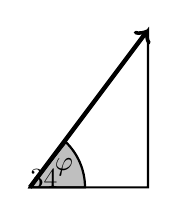
\begin{tikzpicture}[thick]
\coordinate (O) at (0,0);
\coordinate (A) at (1.5,0);
\coordinate (B) at (1.5,2.0);

%\tkzMarkAngle[fill=orange,size=0.5cm, opacity=.4](A,O,B) 
%\tkzLabelAngle[pos=0.8](A,O,B){\texttt{$\varphi$}}
 %%% AAAARGH ovan slutade funka så gjorde nedan HACK i stället
\draw[fill=lightgray, thick] (0,0) -- (0:0.7cm) arc (0:46:0.8cm) node at (30:0.5cm) {$\varphi$} -- cycle;
%\draw[fill=lightgray, thick] (0,0) -- (0:0.7cm) arc (0:45:0.8cm) node at (30:0.5cm) {$\varphi$} -- cycle;
%https://tex.stackexchange.com/questions/96459/automatically-draw-and-labels-angles-of-a-triangle-in-tikz

\draw (O)--(A)--(B)--cycle;
\draw [->, ultra thick] (O)--(B);

\tkzLabelSegment[below=5pt](O,A){\textit{real-delen} är $3$}
\tkzLabelSegment[above left=5pt](O,B){\textit{r}}
\tkzLabelSegment[right=5pt](A,B){\textit{imaginär-delen} är $4$}


\end{tikzpicture}
\end{minipage}

\end{Slide}


\begin{Slide}{Exempel: Klassen Complex}\SlideFontSmall
\scalainputlisting[basicstyle=\ttfamily\SlideFontSize{7}{9}]{../compendium/examples/complex1.scala}
%Klassparametrarna är parametrar till den s.k. \Emph{primärkonstruktorn}.
\begin{REPL}
scala> val z1 = new Complex(3, 4)  // konstruktion av instans av Complex
z: Complex = 3.0 + 4.0i

scala> val polärForm = (z1.r, z1.fi)
polärForm: (Double, Double) = (5.0,0.6435011087932844)

scala> val z2 = Complex(1, 2)   // new behövs inte i Scala 3
z2: Complex = 1.0 + 2.0i

scala> z1 + z2
res0: Complex = 4.0 + 6.0i
\end{REPL}
\url{https://scala-lang.org/api/3.x/scala/math.html#atan2-44b}
\end{Slide}



\begin{Slide}{Exempel: Principen om enhetlig access}\SlideFontSmall
\scalainputlisting[basicstyle=\ttfamily\SlideFontSize{7}{9}]{../compendium/examples/complex2.scala}
\pause
\begin{itemize}
\item Efter som attributen \code{re} och \code{im} är oföränderliga, kan vi lika gärna ändra i klass-implementationen och göra om metoderna \code{r} och \code{fi} till \code{val}-variabler utan att klientkoden påverkas.

\item Då anropas \code{math.hypot} och \code{math.atan2} bara en gång vid initialisering (och inte varje gång som med \code{def}).

\item Vi skulle även kunna använda \code{lazy val} och då bara räkna ut \code{r} och \code{fi} om och när de verkligen refereras av klientkoden, annars inte.

\item Eftersom klientkoden inte ser skillnad på metoder och variabler, kallas detta \Emph{principen om enhetlig access}. (Många andra språk har \Alert{inte} denna möjlighet, tex Java där metoder \emph{måste} ha parenteser.)
\end{itemize}
\end{Slide}



\Subsection{Olika sätt att skapa instanser}

\begin{Slide}{Instansiering med direkt användning av \texttt{new}}

Instansiering genom \Emph{direkt användning} av \code{new}\\
{\SlideFontSmall (här första varianten av Complex med \code{r} och \code{fi} som metoder)}
\begin{REPLnonum}
scala> val c1 = new Complex(3, 4)
\end{REPLnonum}
\begin{tikzpicture}[font=\SlideFontSmall\sffamily]
\matrix [matrix of nodes, row sep=0, column 2/.style={nodes={rectangle,draw,minimum width=0.8cm}}] (mat)
{
\texttt{c1}   &  \makebox(10,10){ }\\
};

\node[cloud, cloud puffs=15.0, cloud ignores aspect, minimum width=2cm, minimum height=3.8cm,
 align=center, draw] (instance1) at (5.8cm, -1.5cm) {
 \begin{tabular}{r l l}
 \texttt{re:} & \texttt{Double} & \fbox{3.0} \\
 \texttt{im:} & \texttt{Double} & \fbox{4.0}\\
 \texttt{imSymbol:} & \texttt{Char} & \fbox{i}\\
 \end{tabular}
 };

\filldraw[black] ($ (mat-1-2) + (0.0cm,0.0cm) $) circle (3pt) node[] (ref1)  {};

\draw [arrow, line width=0.7mm] (ref1) -- (instance1);
\end{tikzpicture}
\pause
Ofta vill man göra \Alert{indirekt} instansiering så att vi senare har friheten att ändra hur instansiering sker.
\end{Slide}



\begin{Slide}{Indirekt instansiering med fabriksmetoder}\SlideFontSmall
En \Emph{fabriksmetod} är en metod som används för att instansiera objekt.
\begin{Code}[basicstyle=\SlideFontSize{8}{12}\ttfamily\selectfont]
object MyFactory {
  def createComplex(re: Double, im: Double) = new Complex(re, im)
  def createReal(re: Double)                = new Complex(re, 0)
  def createImaginary(im: Double)           = new Complex(0, im)
}
\end{Code}
\pause
Instansiera \Alert{inte direkt}, utan \Emph{indirekt} genom användning av \Emph{fabriksmetoder}:
\begin{REPL}
scala> import MyFactory.*

scala> createComplex(3, 4)
res0: Complex = 3.0 + 4.0i

scala> createReal(42)
res1: Complex = 42.0 + 0.0i

scala> createImaginary(-1)
res2: Complex = 0.0 + -1.0i
\end{REPL}
\end{Slide}



\begin{Slide}{Hur förhindra direkt instansiering?}
Om vi vill \Emph{förhindra direkt instansiering} kan vi göra primärkonstruktorn \Alert{privat}:
\scalainputlisting[basicstyle=\ttfamily\SlideFontSize{7}{9}]{../compendium/examples/complex3.scala}
MEN... då går det ju \Alert{inte} längre att instansiera något alls!  \code{   :(}
\begin{REPLnonum}
scala> new Complex(3,4)
error:
 constructor Complex in class Complex cannot be accessed
\end{REPLnonum}
\end{Slide}



\begin{Slide}{Kompanjonsobjekt med indirekt instansiering}\SlideFontSmall
\setlength{\leftmargini}{0pt}
\begin{itemize}
\item Ett \Emph{kompanjonsobjekt} \Eng{companion object} är ett singelobjekt som ligger i \Alert{samma kodfil} som en klass, och som har \Alert{samma namn} som klassen.

\item Medlemmar i ett kompanjonsobjekt \Alert{får accessa privata} medlemmar i kompanjonsklassen (och vice versa) och kompanjonsobjektet får därför accessa privat konstruktor och kan göra \code{new}.

\item Fabriksmetod + privat konstruktor: tillåt \Alert{enbart} \Emph{indirekt instansiering}.
 
\scalainputlisting[basicstyle=\ttfamily\SlideFontSize{7}{9}]{../compendium/examples/complex4.scala}

\item \code{new} behövs för att förhindra rekursivt anrop av \code{apply} och stack overflow
\end{itemize}
\end{Slide}

\begin{Slide}{Användning av kompanjonsobjekt med fabriksmetoder}
Nu kan vi \Alert{bara} instansiera \Emph{indirekt}!  \code{   :)}
\begin{REPLnonum}
scala> Complex.real(42.0)
res0: Complex = 42.0 + 0.0i

scala> Complex.imag(-1)
res1: Complex = 0.0 + -1.0i

scala> Complex.apply(3,4)
res2: Complex = 3.0 + 4.0i

scala> Complex(3,4)
res3: Complex = 3.0 + 4.0i

scala> new Complex(3, 4)
error:
     constructor Complex in class Complex cannot be accessed
\end{REPLnonum}
\end{Slide}


\begin{Slide}{Alternativa direktinstansieringar med default-argument}\SlideFontSmall
Med \Emph{default-argument} kan vi erbjuda \Emph{alternativa} sätt att direktinstansiera.
\scalainputlisting[basicstyle=\ttfamily\SlideFontSize{7}{9}]{../compendium/examples/complex5.scala}
\begin{REPL}
scala> new Complex()
res0: Complex = 0.0 + 0.0i

scala> new Complex(re = 42)  //anrop med namngivet argument
res1: Complex = 42.0 + 0.0i

scala> new Complex(im = -1)
res2: Complex = 0.0 + -1.0i

scala> new Complex(1)
res3: Complex = 1.0 + 0.0i
\end{REPL}
\end{Slide} 

\begin{Slide}{Alternativa sätt att instansiera med fabriksmetod}
Vi kan också erbjuda \Emph{alternativa} sätt att instansiera \Emph{indirekt} med fabriksmetoden \code{apply} i ett kompanjonsobjekt genom default-argument:
\scalainputlisting[basicstyle=\ttfamily\SlideFontSize{7}{9}]{../compendium/examples/complex6.scala}

\end{Slide}

\begin{Slide}{Medlemmar som bara behövs i en enda upplaga}
Attributet \code{imSymbol} passar bättre att ha i \Emph{kompanjonsobjektet}, eftersom det räcker att ha \Alert{en enda upplaga}, som kan vara gemensam för alla objekt:
\scalainputlisting[basicstyle=\ttfamily\SlideFontSize{7}{9}]{../compendium/examples/complex7.scala}

\end{Slide}



\begin{Slide}{Medlemmar i singelobjekt är statiskt allokerade}\SlideFontTiny

Minnesplatsen för \Emph{attribut i singelobjekt} allokeras automatiskt en gång för alla, och kallas därför \Emph{statiskt} allokerad. Singelobjektets namn \code{Complex} utgör en statisk referens till den enda instansen och är av typen \texttt{Complex.type}.

\begin{tikzpicture}[font=\SlideFontSmall\sffamily]
\matrix [matrix of nodes, row sep=0, column 2/.style={nodes={rectangle,draw,minimum width=0.8cm}}] (mat)
{
\texttt{Complex}   &  \makebox(10,10){ }\\
};

\node[cloud, cloud puffs=15.0, cloud ignores aspect, minimum width=1cm, minimum height=2cm,
 align=center, draw] (instance1) at (5.8cm, 0.0cm) {
 \begin{tabular}{r l l}
 \texttt{imSymbol:} & \texttt{Char} & \fbox{i}\\
 \end{tabular}
 };

\filldraw[black] ($ (mat-1-2) + (0.0cm,0.0cm) $) circle (3pt) node[] (ref1)  {};

\draw [arrow, line width=0.7mm] (ref1) -- (instance1);
\end{tikzpicture}

Nu bereder vi inte plats för \code{imSymbol} i varenda \Emph{dynamiskt} allokerade instans:
\begin{REPLnonum}
scala> val c1 = Complex(3, 4)
\end{REPLnonum}

\begin{tikzpicture}[font=\SlideFontSmall\sffamily]
\matrix [matrix of nodes, row sep=0, column 2/.style={nodes={rectangle,draw,minimum width=0.8cm}}] (mat)
{
\texttt{c1}   &  \makebox(10,10){ }\\
};

\node[cloud, cloud puffs=15.0, cloud ignores aspect, minimum width=2cm, minimum height=2cm,
 align=center, draw] (instance1) at (5.8cm, -0.0cm) {
 \begin{tabular}{r l l}
 \texttt{re:} & \texttt{Double} & \fbox{3.0} \\
 \texttt{im:} & \texttt{Double} & \fbox{4.0}\\
 \end{tabular}
 };

\filldraw[black] ($ (mat-1-2) + (0.0cm,0.0cm) $) circle (3pt) node[] (ref1)  {};

\draw [arrow, line width=0.7mm] (ref1) -- (instance1);
\end{tikzpicture}


\end{Slide}




\begin{Slide}{Attribut i kompanjonsobjekt användas för sådant som är gemensamt för alla instanser}

Om vi ändrar på statiska \code{imSymbol} så ändras \code{toString} för \Alert{alla} dynamiskt allokerade instanser.
\begin{REPLnonum}
scala> val c1 = Complex(3, 4)
c1: Complex = 3.0 + 4.0i

scala> Complex.imSymbol = 'j'
Complex.imSymbol: Char = j

scala> val c2 = Complex(5, 6)
c2: Complex = 5.0 + 6.0j

scala> c1
res0: Complex = 3.0 + 4.0j
\end{REPLnonum}
\end{Slide}


\Subsection{Case-klasser och fördelen med oföränderlighet}

\ifkompendium\else
\begin{frame}[plain]
  \includegraphics[width=1.0\textwidth]{../img/mutant.png}
\end{frame}
\fi

\begin{Slide}{Övning: en läskig mutant}\SlideFontSmall
\begin{enumerate}
\item Skapa en klass med namnet \code{Mutant} som har ett förändringsbart attribut som klassparameter med namnet \code{i} av typen \code{Int} med default-argumentet \code{5}.
\vspace{0.5em}

\item \begin{minipage}{0.5\textwidth}
Deklarera två \code{val}-variabler som kallas \code{fem1} och \code{fem2} och som båda refererar till \Alert{samma} \code{Mutant}-instans.
\end{minipage}
\hfill\begin{minipage}{0.32\textwidth}
\hfill\includegraphics[width=3.4cm]{../img/mutant.png}

En \code{Mutant}-instans där \code{i} kanske är fem.
\vspace{1em}
\end{minipage}

\item Skriv kod som ändrar tillstånd via den ena mutantreferensen.

\item Syns ändringen via den andra mutantreferensen?
\end{enumerate}
\end{Slide}




\begin{Slide}{Case-klasser}
Case-klasser är ett smidigt sätt att skapa \Emph{oföränderliga} datastrukturer. Med nyckelordet \code{case} framför \code{class} får du mycket ''godis på köpet'':

\begin{itemize}
\item Klassparametrar blir automatiskt publika\footnote{alltså \Alert{inte} instansprivata som i vanliga klasser.} oföränderliga attribut och du slipper alltså skriva \code{val}.
\item Du får en automatisk \Emph{toString} med klassens namn och värdet av alla \code{val}-attribut som ges av klassparametrarna 
\item och en \Emph{copy}-metod för att skapa nya, delvis förändrade instanser, med attributvärdena som defaultargument.
\item Du får ett automatiskt kompanjonsobjekt med en fabriksmetod \code{apply} för indirekt instansiering där alla klassparametrarnas \code{val}-attribut initialiseras.
\pause
\item ... och mer därtill men mer om det senare...
\end{itemize}
\end{Slide}




\begin{Slide}{Exempel: oföränderliga case-klassen \code{Point}}

\begin{Code}[basicstyle=\SlideFontSize{10}{12}\ttfamily]
case class Point(x: Double, y: Double)
\end{Code}

\begin{REPLnonum}
scala> val p1 = Point(3, 4)
p1: Point = Point(3.0,4.0)

scala> val p2 = p1
p2: Point = Point(3.0,4.0)

scala> p1.x = 42
error: reassignment to val
\end{REPLnonum}
Vi kan utan risk dela med oss av en referens till en oföränderlig klass -- ingen kan ändra dess innehåll. (Jämför läskiga mutanten i tidigare exempel.)

\end{Slide}






\Subsection{Konstruktor}



\begin{Slide}{Vad är en konstruktor?}
\begin{itemize}
\item En \Emph{konstruktor} är den maskinkod som exekveras när klasser instansieras med \code{new}.

\item Konstruktorn skapar ett nytt objekt i minnet vid varje anrop.

\item I Scala \Alert{genererar kompilatorn} en \Emph{primärkonstruktor} åt dig med maskinkod som initialiserar alla attribut baserat på klassparametrarna som du deklarerat.

\pause

%\item I Java och många andra språk får man \Alert{explicit} skriva kod för konstruktorer med speciell syntax och göra alla initialiseringar av attribut själv, och det behövs många olika konstruktorer för att motsvara defaultargument.

\item I Scala \Emph{kan} man också skriva egna alternativa s.k. \Emph{hjälpkonstruktorer}, men det är \Alert{ovanligt}, eftersom man har möjligheten med fabriksmetoder i kompanjonsobjekt och default-argument.
\end{itemize}
\end{Slide}


\begin{Slide}{Hjälpkonstruktorer i Scala (ovanliga)}%\SlideFontSmall
Fördjupning för kännedom:
\begin{itemize}
\item I Scala kan man skapa ett alternativ till primärkonstruktorn, en så kallad \Emph{hjälpkonstruktor} \Eng{auxilliary constructor} genom att deklarera en metod med det speciella namnet \code{this}.


\item Hjälpkonstruktorer \Alert{måste} börja med att anropa en \Alert{annan} konstruktor som står \Alert{före} i koden, till exempel primärkonstruktorn.
\end{itemize}

\begin{Code}
class Point(val x: Int, val y: Int, val z: Int): // primärkonstruktor
  def this(x: Int, y: Int) = this(x, y, 0) // anropa primärkonstruktorn
  def this(x: Int) = this(x, 0) // anropa hjälpkonstruktor
\end{Code}

%{\SlideFontSmall Överlagrade hjälpkonstruktorer i Scala liknar användning av konstruktorer i Java, där man inte har default-argument och apply i kompanjonsobj. etc.}

\end{Slide}

\begin{Slide}{Användning av hjälpkonstruktor}
\begin{REPL}
scala> val p1 = Point(1)
p1: Point = Point@21312342

scala> val p2 = Point(1, 2)
p2: Point = Point@43254325

scala> val p3 = Point(1, 2, 3)
p3: Point = Point@346654
\end{REPL}
\pause
Men man gör \Alert{mycket oftare} så här i Scala:
\begin{Code}[basicstyle=\ttfamily\SlideFontSize{8.5}{12}]
case class Point(x: Int, y: Int = 0, z: Int = 0)
\end{Code}
Använd alltså defaultargument hellre än hjälpkonstruktor.\\
(Eller överlagrad fabriksmetod i kompanjonsobjekt.)
\end{Slide}



% \begin{Slide}{Vad gör skräpsamlaren?}\SlideFontSmall
% \begin{itemize}
% \item Scala och Java är båda programmeringsspråk som förutsätter en körmiljö med \Alert{automatisk}  \Emph{skräpsamling} \Eng{garbage collection}.
%
% \item \Emph{Skräpsamlaren} \Eng{the garbage collector} är ett program som automatiskt körs i bakgrunden då och då och \Emph{städar minnet} genom att frigöra den plats som upptas av \Alert{objekt som inte längre används}.
%
% \item JVM:en bestämmer själv när skräpsamlaren ska jobba och programmeraren har ingen kontroll över detta.
%
% \item Den stora \Emph{fördelen} med automatisk skärpsamling är att man slipper bry sig om det svåra och felbenägna arbetet att \Alert{avallokera} minne.
%
% \item \Alert{Nackdelen} är att man inte kan styra exakt hur och när skräpsamlingen ska ske och man kan därmed inte bestämma när processorn ska belastas med minneshanteringen. Detta är normalt inget problem, utom i vissa tidskritiska realtidssystem med hårda minnesbegränsningar och svarstidskrav.
%
% \item I språk utan automatisk skräpsamling, t.ex. C++, måste man ta hand om destruktion av objekt och skriva egna s.k. \Emph{destruktorer}.
% \end{itemize}
% \end{Slide}


\Subsection{Referens saknas: \texttt{null}}

\begin{Slide}{Referens saknas: \texttt{null}}
\begin{itemize}
\item I Java och många andra språk använder man ofta nyckelordet \code{null} för att representera att ett \Alert{värde saknas}.

\item En referens som är \code{null} refererar inte till någon instans.

\item Om du försöker referera till instansmedlemmar med punktnotation genom en referens som är \code{null} kastas ett \Alert{undantag} \code{NullPointerException}.

\item Oförsiktig användning av \code{null} är en vanlig källa till \Alert{buggar}, som kan vara svåra att hitta och fixa.

\end{itemize}
\end{Slide}


\begin{Slide}{Exempel: \texttt{null}}
\begin{REPL}
scala> class Gurka(val vikt: Int)

scala> var g: Gurka = null        // ingen instans allokerad än
var g: Gurka = null

scala> g.vikt
java.lang.NullPointerException

scala> g = Gurka(42)          // instansen allokeras
g: Gurka = Gurka@1ec7d8b3

scala> g.vikt
val res0: Int = 42

scala> g = null         // instansen kommer att destrueras av skräpsamlaren
\end{REPL}

\begin{itemize} \SlideFontSmall
\item Scala har \code{null} av kompabilitetsskäl, men det är brukligt att \Alert{endast} använda \code{null} om man anropar Java-kod.

\item Scala erbjuder smidiga \code{Option}, \code{Some} och \code{None} för säker hantering av saknade värden; mer om detta kommande vecka.



\end{itemize}
\end{Slide}

\Subsection{Initialisering av attribut}

\begin{Slide}{Defaultvärden under pågående konstruktion}
\begin{tabular}{r | l}
\texttt{Int}    & \texttt{0} \\
\texttt{Double} & \texttt{0.0} \\ \\
\texttt{Float}  & \texttt{0.0F} \\ 
\texttt{Long}   & \texttt{0L} \\ \\
\texttt{Short}  & \texttt{0.toShort} \\
\texttt{Byte}   & \texttt{0.toByte} \\
\texttt{Char}   & \texttt{0.toChar} \\ \\
\texttt{Boolean}   & \texttt{false} \\ \\
Alla referenstyper, tex. \code|String| & \code|null| \\
\end{tabular}
\end{Slide}

\begin{Slide}{Problem med initialisering av attribut vid konstruktion}
\begin{Code}
class InitBug1:  
  val HEJ = hej.toUpperCase
  val hej = "hej"

class InitBug2:
  val b = a
  val a = 10

class InitBug3:
  val hej2 = hej1
  val hej1 = "hej"
\end{Code}
\begin{REPL}
scala> val ib1 = new InitBug1
scala> val ib2 = new InitBug2
scala> ib2.b
scala> val ib3 = new InitBug3
scala> ib3.hej2
\end{REPL}
Vad händer?

\end{Slide}


\begin{Slide}{Vilka värden har attribut medan konstruktion pågår?}
\begin{Code}
class InitBug1:  
  val HEJ = hej.toUpperCase
  val hej = "hej"

class InitBug2:
  var b = a
  var a = 10

class InitBug3:
  val hej2 = hej1
  val hej1 = "hej"
\end{Code}
\begin{REPL}
scala> val ib1 = new InitBug1   // java.lang.NullPointerException
scala> val ib2 = new InitBug2
scala> ib2.b                    // val res0: Int = 0  // WHAT????
scala> val ib3 = new InitBug3
scala> ib3.hej2                 // val res1: String = null  //WHAT???
\end{REPL}
Varför? Vad finns det för lösningar?

\end{Slide}

\begin{Slide}{Hur undvika initialiseringsproblem vid konstruktion?}
\SlideFontSmall
Några tips för att undvika initialiseringsproblem av attribut:
\begin{itemize}
  \item Ändra om möjligt ordningen på attribut-deklarationer
  \item Använd om möjligt i stället \code{lazy val} (init sker senare)
  \item Använd om möjligt i stället \code{def} (evaluering vid varje anrop)
  \item Använd denna kompilatoroption för att få hjälp med varningar vid risk för initialiseringsproblem: \code{-Ysafe-init}
\end{itemize}
\pause
Om du \Alert{verkligen} behöver ha ett oinitialiserat värde:
\begin{Code}
class Box:
  private var x: String = scala.compiletime.uninitialized // tydliggör null-risk
  def get: String = if x != null then x else ""           // glöm ej kolla null
  def getOrElse(alt: String): String = if x != null then x else alt  
  def set(value: String): Unit = x = value
\end{Code}
Försök att \Alert{undvika} \code{null} om det går eftersom det ger stor risk för buggar!\\
{\SlideFontTiny (I ovan fiktiva exempel hade vi kunnat undvika detta enkelt genom att ge x startvärdet \code{""} i stället för null. En sådan lösing förutsätter att det finns en rimlig representation av ett saknat värde. Mer om hantering av saknade värden senare...)}

\end{Slide}

\Subsection{Referensen \texttt{this}}
\begin{Slide}{Referensen \texttt{this}}\SlideFontSmall
\begin{itemize}
\item Nyckelordet \code{this} ger en referens till den aktuella instansen.
\begin{REPLnonum}
scala> class Gurka(var vikt: Int){def jagSjälv = this}

scala> val g = Gurka(42)
val g: Gurka = Gurka@5ae9a829

scala> g.jagSjälv
val res0: Gurka = Gurka@5ae9a829

scala> g.jagSjälv.vikt
val res1: Int = 42

scala> g.jagSjälv.jagSjälv.vikt
val res2: Int = 42
\end{REPLnonum}
\item Referensen \code{this} används ofta för att komma runt ''namnkrockar'' där variabler med samma namn gör så att den ena variabeln inte syns.
\end{itemize}
\end{Slide}



\Subsection{Getters och setters}

\begin{Slide}{Getters och setters}\SlideFontSmall
\begin{itemize}
\item I många språk (t.ex. Java, Python) finns inget motsvarande nyckelord \code{val} som garanterar oföränderliga attributreferenser.
\footnote{Java har visserligen \jcode{final} men det är annorlunda som vi ska se senare.}

\item Därför gör man i dessa språk nästan alltid alla attribut \Alert{privata} för att förhindra att de ändras på ett okontrollerat sätt.

% \item Många språk följer \Alert{inte} principen om enhetlig access: åtkomst av metoder och variabler sker med olika syntax.

\item Därför är det normalt att införa metoder som kallas \Emph{getters} och \Emph{setters}, som används för att \Alert{indirekt} läsa och uppdatera \Emph{attribut}.

\item Dessa metoder känns i många språk igen genom konventionen att de heter något som börjar med \Emph{get} respektive \Emph{set}. (Men \Alert{ej} vanligt i Scala.)

\item Med \Emph{indirekt access} av attribut kan man åstadkomma \Emph{flexibilitet}, så att implementationen kan ändras utan att ändra i klientkoden:
\begin{itemize}\SlideFontSmall
\item[--] man kan t.ex. i efterhand ändra representation av de privata attributen eftersom all access sker genom getters och setters.
\end{itemize}

\item Man kan åstadkomma \Emph{oföränderliga} datastrukturer där attributreferenserna inte förändras efter allokering om klassen \Alert{inte} erbjuder en \Alert{setter} för privata attribut.
\end{itemize}
\end{Slide}



\begin{Slide}{Java-exempel: Klassen JPerson}\SlideFontSmall
\Emph{Indirekt} access av \Alert{privata} attribut:
\vspace{-1em}\begin{multicols}{2}
\javainputlisting[basicstyle=\SlideFontSize{7}{8}\ttfamily\selectfont]{../compendium/examples/JPerson.java}

\columnbreak

\begin{REPLnonum}[basicstyle=\SlideFontSize{7}{9}\ttfamily\color{white}]
$ javac JPerson.java
$ scala
scala> val p = JPerson("Björn")
val p: JPerson = JPerson@7e774085

scala> p.getAge
val res0: Int = 0

scala> p.setAge(42)

scala> p.getAge
val res1: Int = 42

scala> p.age
-- Error:
p.age
^^^^^
value age is not a member of JPerson
\end{REPLnonum}
\end{multicols}
\end{Slide}


\begin{Slide}{Motsvarande JPerson i Scala}
Så här brukar man åstadkomma ungefär motsvarande i Scala: \\~
\begin{Code}[basicstyle=\SlideFontSize{12}{15}\ttfamily\selectfont]
class Person(val name: String):
  var age = 0
\end{Code}
~\\
Notera att alla attribut här är \Emph{publika}.
\end{Slide}


\begin{Slide}{Förhindra felaktiga attributvärden med setters}\SlideFontSmall
Med hjälp av \Emph{setters} kan vi förhindra \Alert{felaktig} uppdatering av attributvärden, till exempel \Alert{negativ ålder} i klassen \code{JPerson} i Java:
\begin{Code}[language=Java]
    public void setAge(int age){
        if (age >= 0) {
            this.age = age;
        } else {
            this.age = 0;
        }
    }
\end{Code}
Hur kan vi åstadkomma \Emph{motsvarande i Scala}? \\
\pause
Antag att vi började med nedan variant, men \Alert{ångrar} oss och sedan vill införa funktionalitet som förhindrat negativ ålder \Emph{utan att ändra i klientkod}:
\begin{Code}
class Person(val name: String):
  var age = 0
\end{Code}
Om vi inför en ny metod \code{setAge} och gör attributet \code{age} privat så funkar det \Alert{inte} längre att skriva  \code{ p.age = 42 } och vi ''kvaddar'' klientkoden! \code{  :(}
\end{Slide}



\begin{Slide}{Getters och setters i Scala}\SlideFontSmall
\setlength{\leftmargini}{0pt}
\begin{itemize}
\item Principen om \Emph{enhetlig access} tillsammans med \Alert{specialsyntax} för \Emph{setters} kommer till vår räddning!

\item
En \Emph{setter} kan i Scala skapas med \textbf{procedur vars namn slutar med} \texttt{\_=}
\pause
\item I Scala kan man utan att kvadda klientkod införa getter+setter så här:
\end{itemize}
\begin{Code}
class Person(val name: String): // ändrad implementation men samma access
  private var myPrivateAge = 0
  def age = myPrivateAge         // getter
  def age_=(a: Int): Unit =      // setter
    if a >= 0 then myPrivateAge = a else myPrivateAge = 0
\end{Code}
\pause\vspace{-0.5em}
\begin{REPL}
scala> val p = Person("Björn")
val p: Person = Person@28ac3dc3

scala> p.age = 42      // najs syntax om getter parad med setter enl ovan
val p.age: Int = 42

scala> p.age = -1      // nu förhindras negativ ålder
val p.age: Int = 0
\end{REPL}
\end{Slide}

%%%%%%%%%%%%%% TODO BORTPRIORITERADE SLIDES NEDAN MEN KANSKE BRA EXEMPEL SOM SKA IN IGEN??? %%%%%%%%%%%%%%%%%%%%

% \begin{Slide}{Med punktnotation kan förändringsbara variabler tilldelas nya värden och objektets tillstånd uppdateras.}
% \begin{REPLnonum}
% scala> björn.ålder = 49
% scala> björn.längd = 178
% \end{REPLnonum}
%
% \begin{tikzpicture}[font=\large\sffamily]
% \matrix [matrix of nodes, row sep=0, column 2/.style={nodes={rectangle,draw,minimum width=0.8cm}}] (mat)
% {
% \texttt{björn}   &  \makebox(10,10){ }\\
% };
% \node[cloud, cloud puffs=13.0, cloud ignores aspect, minimum width=2cm, minimum height=3.8cm,
%  align=center, draw] (x) at (5.8cm, -1.5cm) {
%  \begin{tabular}{r l}
%  \multicolumn{2}{c}{\ttfamily\itshape Person@7ae75ba6}\\ \\
%  \texttt{ålder} & \fbox{~49~~} \\
%  \texttt{längd} & \fbox{~178}\\
%  \end{tabular}
%  };
% \filldraw[black] (0.75cm,0.0cm) circle (3pt) node[] (ref) {};
% \draw [arrow, line width=0.7mm] (ref) -- (x);
% % \node[cloud, cloud puffs=15.7, cloud ignores aspect, %minimum width=5cm, minimum height=2cm,
% % align=center, draw] (g2) at (5cm, -2cm) {Gurka-\\objekt};
% % \filldraw[black] (0.4cm,-0.4cm) circle (3pt) node[] (g2ref) {};
% % \draw [arrow] (g2ref) -- (g2);
% \end{tikzpicture}
% \end{Slide}
%
%
%
%
%
% \begin{Slide}{En klass kan ha parametrar som initialiserar attribut}
% \begin{itemize}
% \item Med en parameterlista efter klassnamnet får man en så kallad \Emph{primärkonstruktor} för initialisering av attribut.
% \item Argumenten för initialiseringen ges vid \code{new}.
% \begin{REPLnonum}
% scala> class Person(var ålder: Int, var längd: Int)
%
% scala> val björn = new Person(49, 178)
% björn: Person = Person@354baab2
%
% scala> println(s"Björn är ${björn.ålder} år gammal.")
% Björn är 49 år gammal.
%
% scala> björn.ålder = 18
%
% scala> println(s"Björn är ${björn.ålder} år gammal.")
% Björn är 18 år gammal.
% \end{REPLnonum}
% \end{itemize}
% \end{Slide}
%
%
%
%
% \begin{Slide}{En klass kan ha privata medlemmar}
% Med \code{private} blir en medlem \Emph{privat}: access utifrån \Alert{medges ej}.
%
% \vspace{0.1em}
% \begin{REPL}
% scala> class Person(private var minÅlder: Int, private var minLängd: Int){
%          def ålder = minÅlder
%        }
%
% scala> val björn = new Person(42, 178)
% björn: Person = Person@4b682e71
%
% scala> println(s"Björn är ${björn.ålder} år gammal.")
% Björn är 42 år gammal.
%
% scala> björn.minÅlder = 18
% error: variable minÅlder in class Person cannot be accessed in Person
%
% scala> björn.längd
% error: value längd is not a member of Person
% \end{REPL}
% Med \code{private} kan man förhindra tokiga förändringar.
% \end{Slide}
%
%
% \begin{Slide}{Privata förändringsbara attribut och publika metoder}
% \begin{Code}
% class Människa(val födelseLängd: Double, val födelseVikt: Double){
%   private var minLängd = födelseLängd
%   private var minVikt  = födelseVikt
%   private var ålder    = 0
%
%   def längd = minLängd  // en sådan här metod kallas "getter"
%   def vikt  = minVikt   // vi förhindrar attributändring "utanför" klassen
%
%   val slutaVäxaÅlder      = 18
%   val tillväxtfaktorLängd = 0.00001
%   val tillväxtfaktorVikt  = 0.0002
%
%   def ät(mat: Double): Unit = {
%     if (ålder < slutaVäxaÅlder) minLängd += tillväxtfaktorLängd * mat
%     minVikt += tillväxtfaktorVikt * mat
%   }
%
%   def fyllÅr: Unit = ålder += 1
%
%   def tillstånd: String = s"Tillstånd: $minVikt kg, $minLängd cm, $ålder år"
% }
% \end{Code}
% \end{Slide}
%
% \begin{Slide}{Tillstånd kan förändras indirekt genom metodanrop}
% \begin{REPL}
% scala> val björn = new Människa(födelseVikt=3.5, födelseLängd=52.1)
% björn: Människa = Människa3e52
%
% scala> björn.tillstånd
% res0: String = Tillstånd: 3.5 kg, 52.1 cm, 0 år
%
% scala> for (i <- 1 to 42) björn.fyllÅr
%
% scala> björn.tillstånd
% res2: String = Tillstånd: 3.5 kg, 52.1 cm, 42 år
%
% scala> björn.ät(mat=5000)
%
% scala> björn.tillstånd
% res3: String = Tillstånd: 4.5 kg, 52.1 cm, 42 år
% \end{REPL}
% \end{Slide}
%
%
%
% \begin{Slide}{Metoden \texttt{isInstanceOf} och rot-typen \texttt{Any}}
% \SlideFontSmall\vspace{-0.5em}
% \begin{multicols}{2}
%
% \begin{REPL}
% scala> class X(val i: Int)
%
% scala> val a = new X(42)
% a: X = X@117b2cc6
%
% scala> a.isInstanceOf[X]
% res0: Boolean = true
%
% scala> val b = new X(42)
% b: X = X@61ab6521
%
% scala> b.isInstanceOf[X]
% res1: Boolean = true
%
% scala> a == b
% res2: Boolean = false
%
% scala> a.i == b.i
% res3: Boolean = true
%
% \end{REPL}
%
% \columnbreak
%
%
% \begin{itemize}\SlideFontTiny
%
% \item Ett objekt skapat med \code{new X} är en instans av \Emph{typen} \code{X}.
%
% \item Detta kan testas med metoden \code{isInstanceOf[X]: Boolean}
%
% \pause
%
% \item Typen \Emph{\texttt{Any}} är sypertyp till \Alert{alla} typer och kallas för \Emph{rot-typ} i Scalas  typhierarki.
%
% \begin{REPL}
% scala> a.isInstanceOf[Any]
% res4: Boolean = true
%
% scala> b.isInstanceOf[Any]
% res5: Boolean = true
%
% scala> 42.isInstanceOf[Any]
% res6: Boolean = true
%
% \end{REPL}
% \item Se quickref sid 4. (Mer i w10.)
% \item I klassen \href{http://www.scala-lang.org/api/current/scala/Any.html}{\code{Any}} finns bl.a. \code{toString}
% \end{itemize}
% \end{multicols}
% \end{Slide}
%
%
%
% \begin{Slide}{Överskugga \texttt{toString}}
% Alla objekt får automatiskt en metod \code{toString} som ger en sträng med objektets unika identifierare, här \texttt{Gurka@3830f1c0}:
% \begin{REPL}
% scala> class Gurka(val vikt: Int)
%
% scala> val g = new Gurka(42)
% g: Gurka = Gurka@3830f1c0
%
% scala> g.toString
% res0: String = Gurka@3830f1c0
% \end{REPL}
% Man kan \Emph{överskugga} den automatiska \code{toString}  med en \Alert{egen implementation}. Observera nyckerordet \code{override}.
% \begin{REPL}
% scala> class Tomat(val vikt: Int){override def toString = s"Tomat($vikt g)"}
%
% scala> val t = new Tomat(142)
% t: Tomat = Tomat(142 g)
%
% scala> t.toString
% res1: String = Tomat(142 g)
%
% \end{REPL}
% \end{Slide}
%
%
%
%
%
% \begin{Slide}{Objektfabrik i kompanjonsobjekt}%\SlideFontSmall
% \begin{itemize}
% \item Om det finns ett objekt i samma kodfil med samma namn som klassen blir det objektet ett s.k.  \Emph{kompanjonsobjekt} \Eng{companion object}.
%
% \item Ett kompanjonsobjekt får \Alert{accessa privata medlemmar} i den klass till vilken objektet är kompanjon.
%
% \item Kompanjonsobjekt är en bra plats för s.k. \Emph{fabriksmetoder} som skapar instanser. Då slipper vi skriva \code{new}.
% \begin{REPL}
% scala> :paste   // måste skrivas tillsammans annars ingen kompanjon
%
% class Broccoli(var vikt: Int)
%
% object Broccoli {
%   def apply(vikt: Int) = new Broccoli(vikt)
% }
%
% scala> val b = Broccoli(420)
% b: Broccoli = Broccoli@32e8d5a4
% \end{REPL}
%
% \end{itemize}
% \end{Slide}
%
%
% \begin{Slide}{Kompanjonsobjekt kan accessa privata medlemmar}%\SlideFontSmall
% \begin{Code}
% class Gurka(startVikt: Double) {
%   private var vikt = startVikt
%   def ät(tugga: Int): Unit = if (vikt > tugga) vikt -= tugga else vikt = 0
%   override def toString = s"Gurka($vikt)"
% }
% object Gurka {
%   private var totalVikt = 0.0
%   def apply(): Gurka = {
%     val g = new Gurka(math.random() * 0.42 + 0.1)
%     totalVikt += g.vikt  // hade blivit kompileringsfel om ej vore kompanjon
%     g
%   }
%   def rapport: String = s"Du har skapat ${totalVikt.toInt} kg gurka."
% }
% \end{Code}
% \pause
% \begin{REPL}
% scala> val gs = Vector.fill(1000)(Gurka())
% gs: scala.collection.immutable.Vector[Gurka] =
%   Vector(Gurka(0.49018400799506734), Gurka(0.2462822679714138), Gurka(0.17391397513818804), Gurka(0.5146514905924656), Gurka(0.47077333689159606)
%
% scala> println(Gurka.rapport)
% Du har skapat 305 kg gurka.
%
% \end{REPL}
%
% \end{Slide}
%
%
%
% \begin{Slide}{Förändringsbara och oföränderliga objekt}
% Ett \Emph{oföränderligt objekt} där nya instanser skapas i stället för tillståndsändring ''på plats''.
% \begin{Code}
% class Point(val x: Int, val y: Int) {
%   def moved(dx: Int, dy: Int): Point = new Point(x + dx, y + dy)
%
%   override def toString: String = s"Point($x, $y)"
% }
% \end{Code}
%
% Ett \Alert{förändringsbart} objekt där \Alert{tillståndet uppdateras}.
% \begin{Code}
% class MutablePoint(private var x: Int, private var y: Int) {
%   def move(dx: Int, dy: Int): Unit = {x += dx; y += dy}  // Mutation!!!
%
%   override def toString: String = s"MutablePoint($x, $y)"
% }
% \end{Code}
% \end{Slide}
%
%
% \begin{Slide}{Oföränderliga objekt}
%
% \begin{minipage}{0.5\textwidth}
% \begin{REPL}
% scala> var p1 = new Point(3, 4)
% p1: Point = Point(3, 4)
%
% scala> val p2 = p1.moved(2, 3)
% p2: Point = Point(5, 7)
%
% scala> println(p1)
% Point(3, 4)
%
% scala> p1 = new Point(0, 0)
% p1: Point = Point(0, 0)
% \end{REPL}
% \end{minipage}
% \pause\begin{minipage}{0.49\textwidth}
% {\SlideFontSmall \hfill Minnessituationen efter rad 7:}
%
% \vspace{1em}
% \begin{tikzpicture}[font=\SlideFontSmall\sffamily,scale=0.75, every node/.style={scale=0.75}]
% \matrix [matrix of nodes, row sep=0, column 2/.style={nodes={rectangle,draw,minimum width=0.6cm}}] (mat)
% {
% \texttt{p1}   &  \makebox(7,7){ }\\
% };
% \node[cloud, cloud puffs=13.0, cloud ignores aspect, minimum width=2cm, minimum height=1cm,
%  align=center, draw] (x) at (3cm, -0.0cm) {
%  \begin{tabular}{r l}
%  \texttt{x} & \fbox{~3~} \\
%  \texttt{y} & \fbox{~4~}\\
%  \end{tabular}
%  };
% \filldraw[black] (0.25cm,0.0cm) circle (3pt) node[] (ref) {};
% \draw [arrow, line width=0.5mm] (ref) -- (x);
% \end{tikzpicture}
%
% \begin{tikzpicture}[font=\SlideFontSmall\sffamily,scale=0.75, every node/.style={scale=0.75}]
% \matrix [matrix of nodes, row sep=0, column 2/.style={nodes={rectangle,draw,minimum width=0.6cm}}] (mat)
% {
% \texttt{p2}   &  \makebox(7,7){ }\\
% };
% \node[cloud, cloud puffs=13.0, cloud ignores aspect, minimum width=2cm, minimum height=1cm,
%  align=center, draw] (x) at (3cm, -0.0cm) {
%  \begin{tabular}{r l}
%  \texttt{x} & \fbox{~5~} \\
%  \texttt{y} & \fbox{~7~}\\
%  \end{tabular}
%  };
% \filldraw[black] (0.25cm,0.0cm) circle (3pt) node[] (ref) {};
% \draw [arrow, line width=0.5mm] (ref) -- (x);
% \end{tikzpicture}
%
% \end{minipage}
%
% \end{Slide}
%
%
%
% \begin{Slide}{Oföränderliga objekt}
%
% \begin{minipage}{0.5\textwidth}
% \begin{REPL}
% scala> var p1 = new Point(3, 4)
% p1: Point = Point(3, 4)
%
% scala> val p2 = p1.moved(2, 3)
% p2: Point = Point(5, 7)
%
% scala> println(p1)
% Point(3, 4)
%
% scala> p1 = new Point(0, 0)
% p1: Point = Point(0, 0)
% \end{REPL}
% \end{minipage}
% \begin{minipage}{0.49\textwidth}
% {\SlideFontSmall \hfill Minnessituationen efter rad 10:}
%
% \vspace{1em}
% \begin{tikzpicture}[font=\SlideFontSmall\sffamily,scale=0.75, every node/.style={scale=0.75}]
% \node[cloud, cloud puffs=13.0, cloud ignores aspect, minimum width=2cm, minimum height=1cm,
%  align=center, draw] (x) at (3cm, 2.0cm) {
%  \begin{tabular}{r l}
%  \texttt{x} & \fbox{~3~} \\
%  \texttt{y} & \fbox{~4~}\\
%  \end{tabular}
%  };
%
%  \node[left of=x, text width=2.5cm,align=right] (text) at (1,2) {kommer att raderas av skräpsamlaren:};
% \end{tikzpicture}
%
% \begin{tikzpicture}[font=\SlideFontSmall\sffamily,scale=0.75, every node/.style={scale=0.75}]
% \matrix [matrix of nodes, row sep=0, column 2/.style={nodes={rectangle,draw,minimum width=0.6cm}}] (mat)
% {
% \texttt{p2}   &  \makebox(7,7){ }\\
% };
% \node[cloud, cloud puffs=13.0, cloud ignores aspect, minimum width=2cm, minimum height=1cm,
%  align=center, draw] (x) at (3cm, -0.0cm) {
%  \begin{tabular}{r l}
%  \texttt{x} & \fbox{~5~} \\
%  \texttt{y} & \fbox{~7~}\\
%  \end{tabular}
%  };
% \filldraw[black] (0.25cm,0.0cm) circle (3pt) node[] (ref) {};
% \draw [arrow, line width=0.5mm] (ref) -- (x);
% \end{tikzpicture}
%
% \begin{tikzpicture}[font=\SlideFontSmall\sffamily,scale=0.75, every node/.style={scale=0.75}]
% \matrix [matrix of nodes, row sep=0, column 2/.style={nodes={rectangle,draw,minimum width=0.6cm}}] (mat)
% {
% \texttt{p1}   &  \makebox(7,7){ }\\
% };
% \node[cloud, cloud puffs=13.0, cloud ignores aspect, minimum width=2cm, minimum height=1cm,
%  align=center, draw] (x) at (3cm, -0.0cm) {
%  \begin{tabular}{r l}
%  \texttt{x} & \fbox{~0~} \\
%  \texttt{y} & \fbox{~0~}\\
%  \end{tabular}
%  };
% \filldraw[black] (0.25cm,0.0cm) circle (3pt) node[] (ref) {};
% \draw [arrow, line width=0.5mm] (ref) -- (x);
% \end{tikzpicture}
%
% \end{minipage}
%
% \pause\vspace{1em}Vi kan \Emph{lugnt dela referenser} till vårt oföränderliga objekt eftersom det \Emph{aldrig} kommer att ändras.
%
% \end{Slide}
%
%
% \newcommand{\MutaVarning}{\vspace{2em}\Alert{Varning!} Vem som helst som har tillgång till en referens till ditt förändringsbara objekt kan \Alert{manipulera} det, vilket ibland ger överaskande och \Alert{problematiska} konsekvenser!}
%
%
%
% \begin{Slide}{Förändringsbara objekt}
%
% \begin{minipage}{0.5\textwidth}
% \begin{REPL}
% scala> val mp1 = new MutablePoint(3, 4)
% mp1: MutablePoint = MutablePoint(3, 4)
%
% scala> val mp2 = mp1
% mp2: MutablePoint = MutablePoint(3, 4)
%
% scala> mp1.move(2,3)
%
% scala> println(mp2)
% MutablePoint(5, 7)
% \end{REPL}
% \end{minipage}
% \begin{minipage}{0.49\textwidth}
% {\SlideFontSmall \hfill Minnessituationen efter rad 4:}
%
% \vspace{1em}
% \begin{tikzpicture}[font=\SlideFontSmall\sffamily,scale=0.75, every node/.style={scale=0.75}]
% \matrix [matrix of nodes, row sep=0.5cm, column 2/.style={nodes={rectangle,draw,minimum width=0.6cm}}] (mat)
% {
% \texttt{mp1}   &  \makebox(7,7){ }\\
% \texttt{mp2}   &  \makebox(7,7){ }\\
% };
% \node[cloud, cloud puffs=13.0, cloud ignores aspect, minimum width=2cm, minimum height=1cm,
%  align=center, draw] (x) at (3cm, -0.0cm) {
%  \begin{tabular}{r l}
%  \texttt{x} & \fbox{~3~} \\
%  \texttt{y} & \fbox{~4~}\\
%  \end{tabular}
%  };
% \filldraw[black] (0.35cm,0.65cm) circle (3pt) node[] (ref1) {};
% \draw [arrow, line width=0.5mm] (ref1) -- (x);
%
% \filldraw[black] (0.35cm,-0.65cm) circle (3pt) node[] (ref2) {};
% \draw [arrow, line width=0.5mm] (ref2) -- (x);
%
%
% \end{tikzpicture}
%
% \end{minipage}
%
% \pause\MutaVarning
% \end{Slide}
%
%
%
%
% \begin{Slide}{Förändringsbara objekt}
%
% \begin{minipage}{0.5\textwidth}
% \begin{REPL}
% scala> val mp1 = new MutablePoint(3, 4)
% mp1: MutablePoint = MutablePoint(3, 4)
%
% scala> val mp2 = mp1
% mp2: MutablePoint = MutablePoint(3, 4)
%
% scala> mp1.move(2,3)
%
% scala> println(mp2)
% MutablePoint(5, 7)
% \end{REPL}
% \end{minipage}
% \begin{minipage}{0.49\textwidth}
% {\SlideFontSmall \hfill Minnessituationen efter \Alert{rad 7}:}
%
% \vspace{1em}
% \begin{tikzpicture}[font=\SlideFontSmall\sffamily,scale=0.75, every node/.style={scale=0.75}]
% \matrix [matrix of nodes, row sep=0.5cm, column 2/.style={nodes={rectangle,draw,minimum width=0.6cm}}] (mat)
% {
% \texttt{mp1}   &  \makebox(7,7){ }\\
% \texttt{mp2}   &  \makebox(7,7){ }\\
% };
% \node[cloud, cloud puffs=13.0, cloud ignores aspect, minimum width=2cm, minimum height=1cm,
%  align=center, draw] (x) at (3cm, -0.0cm) {
%  \begin{tabular}{r l}
%  \texttt{x} & \fbox{~5~} \\
%  \texttt{y} & \fbox{~7~}\\
%  \end{tabular}
%  };
% \filldraw[black] (0.35cm,0.65cm) circle (3pt) node[] (ref1) {};
% \draw [arrow, line width=0.5mm] (ref1) -- (x);
%
% \filldraw[black] (0.35cm,-0.65cm) circle (3pt) node[] (ref2) {};
% \draw [arrow, line width=0.5mm] (ref2) -- (x);
%
%
% \end{tikzpicture}
%
% \end{minipage}
%
% \MutaVarning
% \end{Slide}
%
%
%
% \Subsection{Case-klasser}
%
% \begin{Slide}{Vad är en case-klass?}\SlideFontSmall
% \setlength{\leftmargini}{0pt}
% \begin{itemize}
% \item En \code{case}-klass är ett smidigt sätt att skapa \Emph{oföränderliga objekt}.
% \item Kompilatorn ger dig \Alert{en massa ''godis''} på köpet (ca 50-100 rader kod), inkl.:
% \begin{itemize}\SlideFontTiny
% \item klassparametrar blir automatiskt \code{val}-attribut, alltså \Emph{publika} och \Emph{oföränderliga},
% \item en automatisk \Emph{\texttt{toString}} som visar klassparametrarnas värde,
% \item ett automatiskt \Emph{kompanjonsobjekt} med \Emph{fabriksmetod} så du slipper skriva \code{new},
% \item automatiska metoden \Emph{\texttt{copy}} för att skapa kopior med andra attributvärden, m.m...
% \end{itemize}
%
% \pause
% \item Det \Alert{enda} du behöver göra är att lägga till nyckelordet \code{case} före \code{class}...
% \end{itemize}
%
% \vspace{-0.5em}\begin{REPLnonum}
% scala> case class Point(x: Int, y: Int)
%
% scala> val p = Point(3, 5)
% p: Point = Point(3,5)
%
% scala> p.  // tryck TAB och se lite av allt case-klass-godis
% scala> Point.  // tryck TAB och se ännu mer godis
%
% scala> val p2 = p.copy(y= 30)
% p2: Point = Point(3,30)
% \end{REPLnonum}
%
%
% \end{Slide}
%
%
% \begin{Slide}{Exempel på case-klasser}
% \begin{Code}
% case class Person(namn: String, ålder: Int) {
%   def fyllerJämt: Boolean = ålder % 10 == 0
%   def hyllning = if (fyllerJämt) "Extra grattis!" else "Vi gratulerar!"
%   def ärLikaGammalSom(annan: Person) = ålder == annan.ålder
% }
%
% case class Point(x: Int = 0, y: Int = 0) {
%   def distanceTo(other: Point) = math.hypot(x - other.x, y - other.y)
%   def dx(d: Int): Point = copy(x + d, y)
%   def dy(d: Int): Point = copy(y= y + d)  //namngivet arg. och defaultarg.
% }
% object Point {
%   def origin = new Point()
% }
% \end{Code}
%
% \begin{REPL}
% scala> Point().dx(10).dy(10).dx(32)
% res0: Point = Point(42,10)
%
% scala> Point(3,4) distanceTo Point.origin
% res1: Double = 5.0
%
% \end{REPL}
% \end{Slide}

\input{body/lect-w05-equality.tex}
\input{body/lect-w05-case-classes.tex}
\input{body/lect-w05-specifications.tex}
\input{body/lect-w05-muddiest-point.tex}
\input{body/lect-w05-assignments.tex}

\Lecture{6}{\ModWeekSIX}
%!TEX encoding = UTF-8 Unicode
%!TEX root = ../lect-w06.tex

%%%

\Subsection{Typhierarkier i Scala}

\begin{Slide}{Bastypen för alla typer: \texttt{Any}}
\SlideFontSmall
Scalas typsystem är \Alert{fullständigt}:
\begin{itemize}\SlideFontSmall
  \item Alla värden är objekt som har en typ.
  \item Alla typer är subtyper till bastypen \code{Any}.
  \item Typen \code{Any} kallas därför \Emph{topptyp}.
  \item Alla objekt har vissa grundläggande metoder, så som \code{toString} och \code{==}
\begin{Code}
abstract class Any:
  def getClass
  def isInstanceOf
  def asInstanceOf
  def ==
  def !=
  def ##
  def equals
  def hashCode
  def toString

trait Matchable extends Any
\end{Code}
\end{itemize}

Det kommer mer om abstrakta klasser och traits i veckan om arv.
\end{Slide}

\begin{Slide}{Alla typer är subtyper till \texttt{Any}}\SlideFontSmall\ifkompendium\footnotesize\fi
\vspace{-0.0em}\begin{center}
\newcommand{\TextBox}[1]{\raisebox{0pt}[1em][0.5em]{#1}}
\tikzstyle{umlclass}=[rectangle, draw=black,  thick, anchor=north, text width=2cm, rectangle split, rectangle split parts = 3]
\begin{tikzpicture}[inner sep=0.5em]
\node [umlclass, rectangle split parts = 1, xshift=0cm] (Any)  {
            \textit{\textbf{\centerline{\TextBox{\code{Any}}}}}
        };

\node [umlclass, rectangle split parts = 1, yshift=-1.5cm] (Matchable)  {
            \textit{\textbf{\centerline{\TextBox{\code{Matchable}}}}}
        };



\node [umlclass, rectangle split parts = 1]  at (-2.5cm,-3.25cm) (SubType1) {
            \textbf{\centerline{\TextBox{\code{AnyVal}}}}
            % \nodepart[]{second} \TextBox{\code{val x: A}}
        };

\node [umlclass, rectangle split parts = 1] at (2.5cm,-3.25cm) (SubType2)  {
            \textbf{\centerline{\TextBox{\code{AnyRef}}}}
        };

\draw[umlarrow] (Matchable.north) -- ++(0,0.5) -| (Any.south);
\draw[umlarrow] (SubType1.north) -- ++(0,0.5) -| (Matchable.south);
\draw[umlarrow] (SubType2.north) -- ++(0,0.5) -| (Matchable.south);
\end{tikzpicture}
\end{center}
\begin{itemize}
  \item Alla \Emph{värdetyper}, t.ex. \code{Int}, \code{Double}, \code{Boolean}, är subtyper till \code{AnyVal}
  \item Alla \Emph{referenstyper} t.ex. \code{String} är subtyper till \code{AnyRef}
  \item Värden av typen \code{Matchable} kan användas vid s.k mönstermatchning. 
  \item (Det finns även s.k. opaka typer som inte kan mönstermatchas.)
\end{itemize}
\end{Slide}

\begin{Slide}{Dina egna referenstyper är subtyper till \texttt{AnyRef}}\SlideFontSmall
Alla typer du skapar är subtyper till \code{AnyRef} utan att du behöver skriva det.
\begin{Code}
trait Grönsak:                                 // din egen bastyp
  def vikt: Int

case class Gurka(vikt: Int) extends Grönsak    // din egen subtyp
case class Tomat(vikt: Int) extends Grönsak    // en annan subtyp
\end{Code}
\SlideFontSmall\ifkompendium\footnotesize\fi
\vspace{-0.0em}\begin{center}
\newcommand{\TextBox}[1]{\raisebox{0pt}[1em][0.5em]{#1}}
\tikzstyle{umlclass}=[rectangle, draw=black,  thick, anchor=north, text width=2cm, rectangle split, rectangle split parts = 3]
\begin{tikzpicture}[inner sep=0.5em]
\node [umlclass, rectangle split parts = 1, yshift=-1.5cm] (Base)  {
            \textit{\textbf{\centerline{\TextBox{\code{Grönsak}}}}}
        };



\node [umlclass, rectangle split parts = 1]  at (-2.5cm,-3.5cm) (SubType1) {
            \textbf{\centerline{\TextBox{\code{Gurka}}}}
            % \nodepart[]{second} \TextBox{\code{val x: A}}
        };

\node [umlclass, rectangle split parts = 1] at (2.5cm,-3.5cm) (SubType2)  {
            \textbf{\centerline{\TextBox{\code{Tomat}}}}
        };

\draw[umlarrow] (SubType1.north) -- ++(0,0.5) -| (Base.south);
\draw[umlarrow] (SubType2.north) -- ++(0,0.5) -| (Base.south);
\end{tikzpicture}
\end{center}
Det kommer mer om typhierarkier och \code{extends} i veckan om arv.
\end{Slide}

\Subsection{Mönstermatchning}

\ifkompendium
\noindent  I ett match-uttryck kan man matcha på ett visst värde eller på en viss typ och match-uttryck används gärna istället för nästlade if-uttryck, då de ofta är lättare att läsa och begripa. Med match-uttryck kan man också göra \Emph{mönstermatchning} mot case-klass-instanser, t.ex. för att på ett smidigt sätt undersöka om attribut har speciella värden. Match-uttryck i Scala är en mer kraftfull variant av \code{switch}-satser som finns i många andra språk.  
\fi

\begin{Slide}{Vad är matchning?}

  \begin{itemize}
    \item Matchning gör man då man vill jämföra ett värde mot andra värden och hitta överensstämmelse \Eng{match} enligt olika \Emph{mönster}.
    \item Med mönster kan man även \Alert{plocka isär} objekt i sina beståndsdelar.
  \end{itemize}
\end{Slide}

\begin{Slide}{Plocka isär ett objekt i sina beståndsdelar med mönster}

\begin{REPLnonum}
scala> case class Point(x: Int, y: Int)

scala> val p = Point(1, 2)      // konstruera en punkt
val p: Point = Point(1,2)
\end{REPLnonum}

\pause 

~\\
\begin{REPLnonum}
scala> val Point(x, y) = p      // plocka isär en punkt
val x: Int = 1
val y: Int = 2
  
\end{REPLnonum}
\end{Slide}


\begin{Slide}{Kolla om det passar med nästlade if-uttryck}
Ett vanligt problem: \\ att kolla vilket bland många värden som passar \\~\\

Kan göras med nästlade if-then-else-uttryck:

\begin{Code}
val g = scala.io.StdIn.readLine("Ange en grönsak:")
val smak =
  if g == "gurka" then "gott!"
  else if g == "tomat" then "jättegott!"
  else if g == "broccoli" then "ganska gott..."
  else "inte gott :("

println(g + " är " + smak)
\end{Code}
      
\end{Slide}


\ifkompendium\else
\begin{SlideExtra}{Matchning är ungefär som att passa klossar i en låda}
\includegraphics[width=0.8\textwidth]{../img/plocklada.png}
\end{SlideExtra}
\fi


\begin{Slide}{Kolla om det passar med \texttt{match}-uttryck}\SlideFontSmall
I stället för nästlade \code{if} kan du använda Scalas kraftfulla \code{match}-\Emph{uttryck}:

\begin{Code}
val g = scala.io.StdIn.readLine("Ange en grönsak: ")
val smak = g match 
  case "gurka"    => "gott!"
  case "tomat"    => "jättegott!"
  case "broccoli" => "ganska gott..."
  case _ => "mindre gott..."
\end{Code}
\begin{itemize}
\pause\item Varje \code{case}-gren testas var för sig i tur och ordning \Emph{uppifrån och ned}.
\item Det som står mellan \code{case} och \code{=>} kallas ett \Emph{mönster} \Eng{pattern}
\item Om ett mönster kan matchas så görs det som står efter \code{=>} 
\item \Alert{Inga grenar testas efter lyckad match}.  
\item Sista default-grenen ovan kallas \Emph{wildcard-mönster}: \code{case _ => }
\item Ovan är exempel på matchning mot \Emph{konstant-mönster}, \\ i detta fallet tre stycken strängkonstantmönster.
\item Det finns många andra sätt att skriva mönster.
\end{itemize}
% \pause Scalas \code{match} ''faller inte igenom'' som \code{switch}-satser som finns i många språk, t.ex. Java...

\end{Slide}


\begin{Slide}{Matchning med gard}
Man kan stoppa in en s.k \Emph{gard} \Eng{guard} innan pilen \code{=>} för att villkora matchningen: (notera \code{if} utan \code{then})
\begin{Code}
val g = scala.io.StdIn.readLine("Ange en grönsak: ")
val smak = g match 
  case "gurka" if math.random() > 0.5 => "gott ibland!"
  case "tomat" => "jättegott!"
  case "broccoli" => "ganska gott..."
  case _ => "mindre gott..."
\end{Code}
\code{case}-grenen med gard ger bara en lyckad matchning \\ om uttrycket efter \code{if} är sant; annars provas nästa gren, etc.
\end{Slide}

\begin{Slide}{Matchning med variabelmönster}\SlideFontSmall
Om det finns ett namn efter \code{case} som börjar med liten begynnelsebokstav, blir detta namn en variabel som automatiskt binds till uttrycket före \code{match}:

\begin{Code}
val g = scala.io.StdIn.readLine("Ange en grönsak: ")
val smak = g match 
  case "gurka" if math.random() > 0.5 => "gott ibland!"
  case "tomat" => "jättegott!"
  case "broccoli" => "ganska gott..."
  case other => "smakar bakvänt: " + other.reverse
\end{Code}

Ett \Alert{enkelt} \Emph{variabelmönster}, så som \\ \code{case other => ...} \\ i exemplet ovan, matchar \Alert{allt}! \\\code{other} får alltså värdet av \code{g} om \code{g} \Alert{inte} är \code{"gurka"}, \code{"tomat"}, \code{"broccoli"}.

\end{Slide}


\begin{Slide}{Matchning med eller-mönster}\SlideFontSmall
Om man har samma utfall för olika grenar kan dessa slås ihop och mönstret separeras med vertikalstreck: \code{|}
\begin{Code}
val g = scala.io.StdIn.readLine("Ange en grönsak: ")
val smak = g match 
  case "gurka" => "gott"
  case "tomat" => "gott"
  case "lök"   => "gott"
  case _ => "inte gott"
\end{Code}

Mer koncist med eller-mönster:

\begin{Code}
val g = scala.io.StdIn.readLine("grönsak:")
val smak = g match 
  case "gurka" | "tomat" | "lök" => "gott"
  case _ => "inte gott"
\end{Code}



\end{Slide}





\begin{Slide}{Matchning med typade mönster}\SlideFontSmall
Med en typannotering efter en variabel får man ett \Emph{typat mönster} \Eng{typed pattern}. Om matchningen lyckas blir värdet \Alert{omvandlat} till den specifika typen och binds till variabeln.
\begin{Code}
def f = 
  if math.random() < 0.5 then 42 + math.random() 
  else s"gurka ${math.random()}"

val i = f match 
  case x: Double => x.round.toInt
  case s: String => s.length
\end{Code}
\code{f} får typen \code{Matchable} som är subtyp till \code{Any}. Vilken typ får \code{i}? \pause ~~\code{Int}
{\SlideFontTiny \\\vspace{0.5em} Matchning mot specifika typer enl. ovan används i idiomatisk Scala hellre än \code{isInstanceOf} och \code{asInstanceOf} men man kan göra motsvarande ovan så här:
\begin{Code}
val i2: Int =  
  val x = f
  if x.isInstanceOf[Double] then x.asInstanceOf[Double].round.toInt
  else if x.isInstanceOf[String] then x.asInstanceOf[String].length
  else throw scala.MatchError(x)
\end{Code}
}
\end{Slide}

\begin{Slide}{Typen \text{Matchable}}
\begin{itemize}\SlideFontSmall
\item
När ett uttryck inte kan ges en mer specifik typ så härleds \code{Matchable}, vilket visar att värdet kan undersökas med \code{match}.
\item Exempel: För de orelaterade typerna \code{String} och \code{Double} är den mest specifika typen som kan härledas \code{Matchable}.

\begin{REPLsmall}
scala> def f = if math.random() > 0.5 then 42 else "hej"
def f: Matchable
\end{REPLsmall}

\item Typen \code{Matchable} är nästan lika generell som topptypen \code{Any}. 
\item \code{Matchable} infördes i Scala 3 med \Emph{opaka typalias} som garanterat aldrig boxas men inte kan mönstermatchas. (Ingår ej i denna kurs.)
\item Fördjupning om \code{Matchable} och \code{opaque type} i Scala 3 finns här:
\\\url{https://dotty.epfl.ch/docs/reference/other-new-features}
\end{itemize}
\end{Slide}

\begin{Slide}{Konstruktormönster med case-klasser}\SlideFontSmall
En basklass med gemensamma delar och två subtyper:
\begin{Code}
trait Grönsak:
  def vikt: Int
  def ärRutten: Boolean

case class Gurka(vikt: Int, ärRutten: Boolean) extends Grönsak
case class Tomat(vikt: Int, ärRutten: Boolean) extends Grönsak
\end{Code}
\pause
Tack vare case-klasserna kan man använda \Emph{konstruktormönster} \Eng{constructor pattern} för att se vad som finns \Alert{inuti} en instans:
\begin{Code}
def testa(g: Grönsak): String = g match 
  case Gurka(v, false) => "gott, väger " + v
  case Gurka(_, true)  => "inte gott"
  case Tomat(v, r)     => (if r then "inte " else "") + s"gott, väger $v"
  case _ => s"okänd grönsak: $g"
\end{Code}

Konstruktormönster ''\Emph{plockar isär}'' det som matchas och binder variabler till de attribut som finns i case-klassens konstruktor.
\end{Slide}


\begin{Slide}{Plocka isär samlingar med djupa mönster}
\begin{itemize}
  \item Man kan plocka isär innehållet i en samling så här:
\begin{Code}
def visa(xs: Vector[Grönsak]): String = xs match
  case Vector()               => "tom grönsaksvektor"
  case Vector(Gurka(v, true)) => s"en rutten gurka som väger $v"
  case Vector(g)              => s"exakt en grönsak: $g"
  case Vector(g1, g2)         => s"exakt två grönsaker: $g1, $g2"
  case Vector(g, gs*)         => s"först en $g och sedan svansen: $gs"
\end{Code}
\item Vad händer om du byter ordning på 2:a och 3:e mönstret?
\item \code{Vector(g, gs*)} kan också skrivas som \code{g +: gs}
\end{itemize}
\end{Slide}

\begin{Slide}{Matchning på tupler}
Det går fint att plocka isär tupler med mönstermatchning:\footnote{\url{https://youtu.be/aboZctrHfK8}}
\begin{Code}
var pair = ("hej", 42)

pair match
  case (a, b) if b == 42 => s"livets mening är funnen: $a"
  case (_, b)            => s"fattas mening: $b"

\end{Code}

\end{Slide}

\begin{Slide}{Mönstermatchning och uppräkning med case-objekt}\SlideFontSmall
En bastyp och specifika singelobjekt av gemensam typ:
\begin{Code}
trait Färg
case object Spader  extends Färg // funkar utan case men vi vill ha najs toString
case object Hjärter extends Färg
case object Ruter   extends Färg
case object Klöver  extends Färg

def parallellFärg(f: Färg): Färg = f match
  case Spader  => Klöver
  case Klöver  => Spader
  case Hjärter => Ruter
\end{Code}
Vilken case-gren har vi glömt? Kan kompilatorn hjälpa oss?
\pause
\begin{REPL}
scala> parallellFärg(Ruter)
scala.MatchError: Ruter 
\end{REPL}
\Alert{Undantag vid körtid} \code{:(}
\end{Slide}

\begin{Slide}{Mönstermatchning och förseglade typer}\SlideFontSmall
Med nyckelordet \code{sealed} får vi en kompileringsvarning.
\begin{Code}
sealed trait Färg //tryck Alt+Enter i REPL för tolkning av flera rader ett svep
case object Spader  extends Färg
case object Hjärter extends Färg
case object Ruter   extends Färg
case object Klöver  extends Färg

def parallellFärg(f: Färg): Färg = f match 
  case Spader  => Klöver
  case Klöver  => Spader
  case Hjärter => Ruter
\end{Code}
\begin{REPL}
1 |def parallellFärg(f: Färg): Färg = f match 
  |                                   ^
  |                           match may not be exhaustive.
  |
  |                           It would fail on pattern case: Ruter
def parallellFärg(f: Färg): Färg
\end{REPL}
\Emph{Varning vid kompilering} \code{:)} ~~~Sista raden visar att det bara är en varning!
\end{Slide}

\begin{Slide}{Mönstermatcha enumeration}\SlideFontSmall
I stället för \code{sealed trait ... case object ...} kan du använda en \Emph{enumeration} (ä.k. uppräkning, uppräknad datatyp, \Eng{enumeration}).
\begin{Code}
enum Färg:
  case Spader, Hjärter, Ruter, Klöver
  
def parallellFärg(f: Färg): Färg = 
  import Färg.*
  f match 
    case Spader  => Klöver
    case Klöver  => Spader
    case Hjärter => Ruter
\end{Code}
\pause
\begin{REPL}
def parallellFärg(f: Färg): Färg
3 |  f match 
  |  ^
  |  match may not be exhaustive.
  |
  |  It would fail on pattern case: Ruter
\end{REPL}
\Emph{Även här får vi hjälpsam varning vid kompilering} \code{:)} 
\end{Slide}

\begin{Slide}{Stora/små begynnelsebokstäver vid matchning}
\Alert{Fallgrop}: matcha \Alert{värde} som börjar med \Alert{liten} bokstav.
\begin{REPL}
scala> val livetsMening = 42

scala> def ärLivetsMeningBuggig(svar: Int) = svar match 
         case livetsMening => true    // lokalt namn som matchar allt!
         case _ => false

scala> ärLivetsMeningBuggig(43)
val res0: Boolean = true

scala> val LivetsMening = 42   // stor begynnelsebokstav

scala> def ärLivetsMening(svar: Int) = svar match 
         case LivetsMening => true    // funkar fint!
         case _ => false

scala> ärLivetsMening(43)
val res1: Boolean = false
\end{REPL}
\end{Slide}


\begin{Slide}{Stora/små begynnelsebokstäver vid matchning}
Ett sätt att komma runt problemet med liten begynnelsebokstav: \\
\Emph{backticks} to the rescue!
\begin{REPL}
scala> val livetsMening = 42

scala> def ärLivetsMeningBackTicks(svar: Int) = svar match 
         case `livetsMening` => true    // nu funkar det!
         case _ => false

scala> ärLivetsMeningBackTicks(43)
val res2: Boolean = false
\end{REPL}
\end{Slide}

\ifkompendium\else
\begin{Slide}{Mönster på andra ställen än i \texttt{match}}\SlideFontSmall
Mönster i \Emph{deklarationer}:
\vspace{-0.25em}\begin{REPL}
scala> case class Point(x: Int, y: Int)

scala> val p = Point(0, 1)

scala> val Point(x, y) = p          // konstruktormönster med case-klass
val x: ???
val y: ???

scala> val (x, y, z) = (0, 1, 2)    // konstruktormönster med tupel
val x: ???
val y: ???
val z: ???

\end{REPL}
Mönster i \Emph{for-uttryck}:
\vspace{-0.25em}\begin{REPL}
scala> val xs = for (x, y) <- Vector((1,2), (3,4)) yield x
val xs: ???
\end{REPL}

\end{Slide}
\fi

\begin{Slide}{Mönster på andra ställen än i \texttt{match}}\SlideFontSmall
Mönster i \Emph{deklarationer}:
\vspace{-0.25em}\begin{REPL}
scala> case class Point(x: Int, y: Int)

scala> val p = Point(0, 1)

scala> val Point(x, y) = p          // konstruktormönster med case-klass
val x: Int = 0
val y: Int = 1

scala> val (x, y, z) = (0, 1, 2)    // konstruktormönster med tupel
val x: Int = 0
val y: Int = 1
val z: Int = 2

\end{REPL}
Mönster i \Emph{for-uttryck}:
\vspace{-0.25em}\begin{REPL}
scala> val xs = for (x, y) <- Vector((1,2), (3,4)) yield x
val xs: Vector[Int] = Vector(1, 3)
\end{REPL}
\end{Slide}

\begin{Slide}{Mönsterdelar och variabelt antal argument}\SlideFontSmall
Met två olika specialtecken går det att
\begin{itemize}
\item binda variabler till \Emph{mönsterdelar} med \code{@} \\
\code{case Vector(xs@Vector(a), Vector(42)) => ...}

\item matcha \Emph{variabelt antal argument}  med \code{*}  
\\ \code{case Vector(a, _, c) => ... }  matchar om 3 element, \_ kvittar
\\ \code{case Vector(a, svans*) => ... }  matchar om minst ett element
\\ \code{case Vector(a, _*) => ... }  intresserad av första, svans kvittar
\end{itemize}
%Läs mer om mönster här: \url{https://docs.scala-lang.org/scala3/book/taste-control-structures.html#match-expressions}
\end{Slide}


\begin{Slide}{Partiella funktioner och metoden \texttt{collect}}\SlideFontSmall
\begin{itemize}
\item En \Alert{partiell} \Emph{funktion} är, till skillnad från en \Alert{total} \Emph{funktion}, inte definierad för alla parametervärden.
\item Partiella funktioner kan skapas med \code{case} utan \code{match}:
\begin{Code}
val pf: PartialFunction[Int, Double] = case z if z != 0 => 1.0 / z  
\end{Code}
\item  Funktionen är inte definierad för argumentet \code{0}:

\begin{REPLsmall}
scala> pf(0)                         
scala.MatchError: 0 
\end{REPLsmall}
\item 
Detta är användbart tillsammans med samlingsmetoden \code{collect} som  applicerar en partiell funktion endast på definierade värden: 
\begin{REPLsmall}
scala> Vector(1, 2, 0, 4).collect(pf)
val res0: Vector[Double] = Vector(1.0, 0.5, 0.25)

scala> Vector(1 -> 2, 0 -> 3, 42 -> 0).collect{ case (a,b) if a > 0 => a } 
val res1: Vector[Int] = Vector(1, 42)

\end{REPLsmall}
Notera att \Alert{krullparentes behövs} vid ensamt \code{case} som argument.
% \item Läs mer om mönster här:  \href{http://www.artima.com/pins1ed/case-classes-and-pattern-matching.html}{\SlideFontTiny www.artima.com/pins1ed/case-classes-and-pattern-matching.html}

% \item För djupare förståelse av hur \code{case} fungerar, läs speciellt om \Emph{partiella funktioner} här: \href{http://www.artima.com/pins1ed/case-classes-and-pattern-matching.html\#15.7}{\SlideFontTiny www.artima.com/pins1ed/case-classes-and-pattern-matching.html\#15.7}

% \item Läs om extractors här: \href{http://www.artima.com/pins1ed/extractors.html}{\SlideFontTiny www.artima.com/pins1ed/extractors.html}

\end{itemize}
\end{Slide}


\begin{Slide}{Fördjupning: metoden \texttt{unapply}}\SlideFontSmall
När du deklarerar en case-klass kommer kompilatorn att \Alert{automatiskt generera en metod} med namnet \Emph{\texttt{unapply}}.
\begin{REPL}
scala> case class Gurka(vikt: Int, ärRutten: Boolean)

scala> Gurka.unapply // tryck ENTER för att se typen
val res0: Gurka => Gurka = Lambda1914/0x00000008408cf840@b0e7bde

scala> val g = Gurka(100, false)

scala> Gurka.unapply(g)
val res1: Gurka = Gurka(100,false)
\end{REPL}
\textbf{Vad ska detta vara bra för?} \pause 
Metoden \code{unapply} genereras av kompilatorn och används internt vid matchning och det är den metoden som gör att case-klasser kan användas i konstruktormönster. Principen är generell: Man kan skapa \Emph{egna} s.k. \Alert{extraktorer} \Eng{extractors} som kan plocka isär ett värde med mönstermatchning, även utan case-klass. \\För den nyfikne: \url{https://docs.scala-lang.org/scala3/reference/changed-features/pattern-matching.html} 
\end{Slide}

%!TEX encoding = UTF-8 Unicode
%!TEX root = ../lect-w06.tex

%%%


\ifkompendium\else
%\Subsection{Kapsla in speciella värden: Option[kanske saknas] och Try[kanske misslyckas]}
\Subsection{Hantera speciella värden med inkapsling}

{
\setbeamertemplate{navigation symbols}{}
\setbeamercolor{background canvas}{bg=black}
\begin{frame}[plain]
    \color{white}{Inkapsling av speciella värden så att krasch kan undvikas}
    \makebox[\linewidth]{\includegraphics[width=\paperwidth]{../img/crystal.jpg}}
\end{frame}
}
\fi

\Subsection{Hantera saknade värden med \texttt{Option}}

\begin{Slide}{Hur hantera saknade värden?}\SlideFontSmall
Olika sätt att hantera saknade värden:
\begin{itemize}
\item Hitta på ett specialvärde: exempel -1 för saknat värde
\item \code{null} om värde saknas (vanligt i Java m.fl. språk, mkt ovanligt i Scala)
\item Använd en samling och låt tom samling representera saknat värde: \\
\code{val sums = Vector(Vector(42),Vector(32),Vector(),Vector(21))}

\item \code{Option[A]} gemensam bastyp för: \\
  \code{None} som representerar \Alert{saknat värde}, och \\ \code{Some[A]} som representerar att \Emph{värde finns}
\end{itemize}
\end{Slide}



\begin{Slide}{En gemensam bastyp för ett värde som kanske saknas}\SlideFontSmall\ifkompendium\footnotesize\fi
\vspace{-0.0em}\begin{center}
\newcommand{\TextBox}[1]{\raisebox{0pt}[1em][0.5em]{#1}}
\tikzstyle{umlclass}=[rectangle, draw=black,  thick, anchor=north, text width=3cm, rectangle split, rectangle split parts = 3]
\begin{tikzpicture}[inner sep=0.5em]
\node [umlclass, rectangle split parts = 2, xshift=0cm, text width=3.5cm] (BaseType)  {
            \textit{\textbf{\centerline{\TextBox{\code{Option[A]}}}}}
            \nodepart[]{second}
            \TextBox{\code{def get: A}}\newline
            \TextBox{\code{def isEmpty: Boolean}}

        };

\node [umlclass, rectangle split parts = 1]  at (-2.5cm,-3.0cm) (SubType1) {
            \textbf{\centerline{\TextBox{\code{Some[A]}}}}
            % \nodepart[]{second} \TextBox{\code{val x: A}}
        };

\node [umlclass, rectangle split parts = 1] at (2.5cm,-3.0cm) (SubType2)  {
            \textbf{\centerline{\TextBox{\code{None}}}}
        };
\draw[umlarrow] (SubType1.north) -- ++(0,0.5) -| (BaseType.south);
\draw[umlarrow] (SubType2.north) -- ++(0,0.5) -| (BaseType.south);
\end{tikzpicture}
\end{center}
\pause
\vspace{-0.5em}\begin{REPL}
scala> var x: Option[Int] = Some(42)

scala> x.isEmpty
val res0: Boolean = false

scala> x = None

scala> x.isEmpty
val res1: Boolean = true
\end{REPL}
\end{Slide}


\begin{Slide}{Option för hantering av ev. saknade värden}\SlideFontSmall
Alla vill inte berätta för Facebook vad de har för kön. \\ Förbättra Facebooks kod med ett litet Scala-program:
\begin{Code}
enum Gender:
  case Man, Woman

case class Person(name: String, gender: Option[Gender])
\end{Code}
\pause
\begin{REPL}
scala> val p1 = Person("Björn",  Some(Gender.Man))
scala> val p2 = Person("Sandra", Some(Gender.Woman))
scala> val p3 = Person("Kim",  None)
scala> val g2 = p2.gender
scala> def show(g: Option[Gender]): String = g match {
         case Some(x) => x.toString
         case None    => "unknown"
       }
scala> show(g2)
scala> show(p3.gender)
scala> val ps = Vector(p1,p2,p3)
scala> ps.map(_.gender).map(show)   // None ignoreras av map
\end{REPL}
\end{Slide}

\begin{Slide}{Några smidiga metoder på \code{Option}}\SlideFontSmall
Metoden \code{getOrElse} gör att man ofta kan undvika matchning.
\begin{Code}
var opt: Option[Int] = None

val x = opt.getOrElse(42)   // get the value, give default if missing
\end{Code}

Flera av de vanliga samlingsmetoderna funkar, t.ex. \code{foreach} och \code{map}.
\begin{Code}
opt.foreach(x => println(x)) // only done if value exists

opt.map(x => x + 1)          // only done if value exists

opt = Some(42)               // change opt to now have some value

opt.foreach(x => println(x)) // done as value now exists

opt.map(x => x + 1)          // done as value now exists

\end{Code}
\end{Slide}


\begin{Slide}{Några samlingsmetoder som ger en \code{Option}, övning}
\begin{REPL}
scala> val (xs, ys) = (Vector(1,2,3), Vector())

scala> xs.headOption
res0: ???

scala> ys.headOption
res1: ???

scala> xs.find(_ > 1)
res2: ???

scala> xs.find(_ > 5)
res3: ???

scala> val huvudstad = Map("Sverige" -> "Sthlm", "Skåne" -> "Malmö")

scala> huvudstad.get("Skåne")
res4: ???

scala> huvudstad.get("Danmark")
res5: ???
\end{REPL}
\end{Slide}

\begin{Slide}{Några samlingsmetoder som ger en \code{Option}, svar}
\begin{REPL}
scala> val (xs, ys) = (Vector(1,2,3), Vector())

scala> xs.headOption
res0: Option[Int] = Some(1)

scala> ys.headOption
res1: Option[Nothing] = None

scala> xs.find(_ > 1)
res2: Option[Int] = Some(2)

scala> xs.find(_ > 5)
res3: Option[Int] = None

scala> val huvudstad = Map("Sverige" -> "Sthlm", "Skåne" -> "Malmö")

scala> huvudstad.get("Skåne")
res4: Option[String] = Some(Malmö)

scala> huvudstad.get("Danmark")
res5: Option[String] = None
\end{REPL}
\end{Slide}

%!TEX encoding = UTF-8 Unicode
%!TEX root = ../lect-w06.tex

%%%



\Subsection{Undantag}

\ifkompendium\else
\begin{SlideExtra}{Undantag kan orsaka krasch...}
\includegraphics[width=1.0\textwidth]{../img/dynamite}  
\end{SlideExtra}

\begin{SlideExtra}{Undantag orsakar ingen krasch om inkapslad i en Try}
\hspace{0.3\textwidth}\includegraphics[width=0.6\textwidth,angle=-90,origin=c]{../img/bomb-shelter}  
\end{SlideExtra}
\fi

\begin{Slide}{Vad är ett undantag \Eng{exception}?}
Undantag representerar ett fel eller ett onormalt tillstånd som upptäcks under exekvering och som  behöver hanteras på särskilt sätt vid sidan av det normala exekveringsflödet.

\vspace{1em}\href{https://sv.wikipedia.org/wiki/Undantagshantering}{sv.wikipedia.org/wiki/Undantagshantering}


\vspace{1em} Exempel på undantag:

\pause

\begin{itemize} \SlideFontSmall
\item Indexering utanför vektorns indexgränser.

\item Läsning bortom filens slut.

\item Försök att öppna en fil som inte finns.

\item Minnet är slut.

\item Heltalsdivision med noll ger \code{java.lang.ArithmeticException}.

\item \code{"hej".toInt} ger \code{java.lang.NumberFormatException}

\end{itemize}

\end{Slide}


\begin{Slide}{Orsaka undantag indirekt med \texttt{require} och \texttt{assert}}

\begin{itemize}\SlideFontSmall
  \item Med funktionen \code{require(b)} skapas ett \\\code{IllegalArgumentException("requirement failed")} \\ om \code{b} är \code{false}
  \item \code{require} används om man vill begränsa vilka argument som är giltiga
  \item Med funktionen \code{assert(b)} skapas ett \code{AssertionError("assertion failed")} \\ om \code{b} är \code{false} 
  \item \code{assert} används om man vill förhindra ogiltiga tillstånd
\end{itemize}
{
  \ifkompendium\else
  \vfill\SlideFontTiny
  \fi
  Se implementationen av \code{require} här:\\
\url{https://github.com/scala/scala/blob/v2.13.6/src/library/scala/Predef.scala#L315}
}
\end{Slide}

\begin{Slide}{Kasta dina egna undantag med \texttt{throw}}\SlideFontSmall
Man kan själv generera ett undantag med \code{throw}, vilket kallas att \Emph{kasta} ett undantag som (om det inte \Emph{fångas}), gör att exekveringen \Alert{avbryts}.


\begin{REPL}
scala> def pang = throw Exception("PANG!")
pang: Nothing

scala> pang
java.lang.Exception: PANG!

\end{REPL}
\pause
Olika sätt att hantera undantag och förhindra att exekveringen avbryts:
\begin{itemize}
\item \code{try catch}-uttryck omvandlar undantag till ngt lämpligt värde.
%\item Java: Man kan använda en \code{try ... catch}-sats och \Alert{göra något} i händelse av undantag.

\item \texttt{scala.util.Try} \Emph{kapslar in} kod som kan ge undantag.  %(Finns ej i Java; att föredra i Scala.)
\end{itemize}
\end{Slide}


\Subsection{Hantera undantag med \texttt{Try}}

\begin{Slide}{En gemensam bastyp för något som kan misslyckas}\SlideFontSmall
\begin{Code}
import scala.util.{Try, Success, Failure}
\end{Code}
\ifkompendium\footnotesize\fi
\vspace{-0.5em}\begin{center}
\newcommand{\TextBox}[1]{\raisebox{0pt}[1em][0.5em]{#1}}
\tikzstyle{umlclass}=[rectangle, draw=black,  thick, anchor=north, text width=3.0cm, rectangle split, rectangle split parts = 3]
\begin{tikzpicture}[inner sep=0.5em]
\node [umlclass, rectangle split parts = 2, xshift=0cm, text width=3.8cm] (BaseType)  {
            \textit{\textbf{\centerline{\TextBox{\code{Try[T]}}}}}
            \nodepart[]{second}
            \TextBox{\code{def get: T}}\newline
            \TextBox{\code{def isFailure: Boolean}}\newline
            \TextBox{\code{def isSuccess: Boolean}}
        };

\node [umlclass, rectangle split parts = 2, text width=2.2cm]  at (-2.5cm,-3.7cm) (SubType1) {
            \textbf{\centerline{\TextBox{\code{Success[T]}}}}
            \nodepart[]{second} \TextBox{\code{val value: T}}
        };

\node [umlclass, rectangle split parts = 2, text width=4.2cm] at (2.5cm,-3.7cm) (SubType2)  {
            \textbf{\centerline{\TextBox{\code{Failure[T]}}}}
            \nodepart[]{second} \TextBox{\code{val exception: Throwable}}
        };
\draw[umlarrow] (SubType1.north) -- ++(0,0.5) -| (BaseType.south);
\draw[umlarrow] (SubType2.north) -- ++(0,0.5) -| (BaseType.south);
\end{tikzpicture}
\end{center}
\end{Slide}

\begin{Slide}{Hantera undantag med \texttt{Try}}
\vspace{-0.5em}\begin{REPLsmall}
scala> def pang = throw new Exception("PANG!")

scala> def kanskePang = if math.random() < 0.5 then 42 else pang

scala> import scala.util.{Try, Success, Failure}

scala> def försök = Try { kanskePang }

scala> val xs = Vector.fill(15){försök}

scala> val trettonde = xs(12) match
         case Success(value) => value
         case Failure(e) => println(e); -1

scala> (xs(12).isSuccess, xs(12).isFailure) 

scala> xs(12).getOrElse(0)

scala> xs(12).toOption

scala> försök.foreach(println)

scala> försök.map(_ + 1)

scala> for Success(x) <- xs yield x
\end{REPLsmall}
\end{Slide}

\Subsection{Hantera undantag med \texttt{try}-\texttt{catch}}


\begin{Slide}{\texttt{try}-\texttt{catch}-uttryck}\SlideFontSmall
Man kan fånga undantag med ett \code{try ... catch}-uttryck:
\begin{Code}
def carola = 
  try 
    if math.random() > 0.5 then throw Exception("stormvind")
    42
  catch 
    case e: Exception =>
      println("Fångad av en " + e.getMessage)
      -1

\end{Code}
\pause
\begin{REPL}
scala> Vector.fill(5)(carola)
Fångad av en stormvind
Fångad av en stormvind
Fångad av en stormvind
val res0: Vector[Int] = Vector(-1, 42, 42, -1, -1)
\end{REPL}
%Gör uppg. 9-11 i övn. \code{patterns} som visar hur man fångar undantag i Scala och Java. 
%Mer om undantag i fortsättningskursen.
\end{Slide}

\Subsection{För- och nackdelar med undantag}

\begin{Slide}{Unvik undantag om det går}
\SlideFontSmall
\Emph{Fördelar} med undantag: 
\begin{itemize}
\item Vid allvarliga fel då det inte är mycket att göra än att starta om, t.ex. \code{OutOfMemoryException}, är det bra att få veta vad som är fel.
\item Onormala fall som uppkommer sällan kan hanteras separat (t.ex. i huvudprogrammet) utan att koden för normalfallet blir tillkrånglad. 
\end{itemize}
\Alert{Nackdelar} med undantag: 
\begin{itemize}
\item Ett slags ''goto'' som gör exekveringsflödet svårt att följa.
\item Skapa stack-trace tar tid; undantag som sker ofta påverkar prestanda.
\end{itemize}
\pause Exempel: undantagslösa \code{toIntOption} är både säker och snabb!
\begin{REPLsmall}
scala> def time(op: => Unit): Long = {val t0 = System.nanoTime; op; System.nanoTime - t0}

scala> def min(op: => Unit, n: Int = 1000): Long = Seq.fill(n)(time(op)).drop(n / 20).min

scala> min(util.Try("hello".toInt))
val res0: Long = 3549

scala> min(try "hello".toInt catch (_: Throwable) => ())
val res1: Long = 3046

scala> min("hello".toIntOption)
val res2: Long = 157
\end{REPLsmall}
\end{Slide}

\begin{Slide}{Fördjupning: Kontrollerade undantag}
\begin{itemize}
\item Det finns möjligheter i Scala att låta kompilatorn kontrollera om undantag hanteras.
\item Läs mer här: \\ \url{https://docs.scala-lang.org/scala3/reference/experimental/canthrow.html}
\end{itemize}
  
\end{Slide}
\input{body/lect-w06-equals.tex}
\input{body/lect-w06-assignments.tex}

\Lecture{7}{\ModWeekSEVEN}
%!TEX encoding = UTF-8 Unicode
%!TEX root = ../lect-w07.tex

\Subsection{Vad är en sekvens?}

\ifkompendium\else
{
  \setbeamercolor{background canvas}{bg=black}
  \frame[plain]{\centering\Huge\textbf{\color{pink}{ORDNINGEN}\\SPELAR\\ROLL}}
}
\fi


\begin{Slide}{Vad är en sekvens?}  
\begin{itemize}
\item En sekvens är en \Emph{följd av element} som
  \begin{itemize}
  \item har \Alert{ordningsnummer} (t.ex. numrerade från noll)
  \item är av en viss \Alert{typ} (t.ex. heltal).
  \end{itemize}
  \pause
\item En sekvens kan innehålla flera element som är lika.
\item En sekvens kan vara \Alert{tom} och har då längden noll.
\item Exempel på en icke-tom sekvens med dubbletter:
\begin{REPLnonum}
scala> val xs = Vector(42, 0, 42, -9, 0, 5)
xs: scala.collection.immutable.Vector[Int] =
  Vector(42, 0, 42, -9, 0, 5)
\end{REPLnonum}
\pause
\item \Emph{Indexering} ger ett element via dess ordningsnummer:
\begin{REPLnonum}
scala> xs(2)
res0: Int = 42

scala> xs.apply(2)
res1: Int = 42
\end{REPLnonum}
\end{itemize}
\end{Slide}

\begin{Slide}{Exempel: En sträng är en sekvens av tecken}
\begin{REPLnonum}
scala> "haj po daj"
\end{REPLnonum}
Längd? 
Vad ligger på första platsen?
Elementtyp?
Dubbletter?
\pause
\begin{REPLnonum}
scala> "haj po daj".length
res1: Int = 10

scala> "haj po daj".apply(0)
res2: Char = h

scala> "haj po daj"(0)
res3: Char = h

scala> "haj po daj".distinct
res4: String = haj pod
\end{REPLnonum}

\end{Slide}


\begin{Slide}{Iterera över element i en sekvens}
\begin{itemize}
\item Att \Emph{iterera} \Eng{iterate}, ä.k. traversera \Eng{traverse}, innebär att \Alert{gå igenom} och behandla element i en samling. 
\item Exempel på iterering med \code{foreach}, \code{map}, \code{for}:
\begin{REPLnonum}
scala> val xs = Vector(1,2,3)
val xs: Vector[Int] = Vector(1, 2, 3)

scala> xs.foreach(x => println(x + 1)) 
2
3
4

scala> xs.map(_ + 1)
val res0: Vector[Int] = Vector(2, 3, 4)

scala> for x <- xs yield x - 1
val res1: Vector[Int] = Vector(0, 1, 2)

\end{REPLnonum}
\end{itemize}
\end{Slide}

\begin{Slide}{Lägg till i början och i slutet av en sekvens}
  \begin{itemize}
  \item Med metoderna \code{+:} och \code{:+} kan du skapa en ny sekvens med nya element tillagda i början resp. i slutet.
  \item Minnesregel: ''\Alert{Colon on the collection side}''
  \begin{REPLnonum}
  scala> val xs = Vector(1,2,3)
  scala> 42 +: xs         // ger ny Vector(42, 1, 2, 3)
  scala> xs :+ 42         // ger ny Vector(1, 2, 3, 42)
  \end{REPLnonum}
  \pause
  \item Semantik: operatornotation med operatorer som \Emph{slutar med kolon} är \Alert{högerassociativa}
  \item Anropet \code{42 +: xs} skrivs av kompilatorn om till \code{xs.+:(42)}
  \begin{REPL}
  scala> xs.+:(42)
  res4: scala.collection.immutable.Vector[Int] = Vector(42, 1, 2, 3)
  \end{REPL}
  \pause
  \item Konkatenering (sammanfogning) av sekvenser: \code{xs ++ ys}
  
  \end{itemize}
\end{Slide}


\begin{Slide}{Egenskaper hos några sekvenssamlingar i Scala}
\vspace{-0.5em}
\begin{itemize}\SlideFontSmall

\item \code{Vector}
  \begin{itemize}\SlideFontSmall
  \item \Emph{Oföränderlig}. Snabb på att skapa kopior med små förändringar.
  \item Allsidig prestanda: \Emph{bra till det mesta}.
  \end{itemize}

\item \code{List}
  \begin{itemize}\SlideFontSmall
  \item \Emph{Oföränderlig}. Snabb på att skapa kopior med små förändringar.
  \item Snabb indexering \& uppdatering \Emph{i början}.
  \item Smidig \& snabb vid \Emph{rekursiva} algoritmer.
  \item Långsam vid upprepad \Alert{indexering} på godtyckliga ställen.
  \end{itemize}

\item \code{ArrayBuffer}
  \begin{itemize}\SlideFontSmall
  \item \Alert{Föränderlig}: \Emph{snabb indexering \& uppdatering}.
  \item Kan \Emph{ändra storlek} efter allokering. Snabb att indexera överallt.
  \end{itemize}

\item \code{ListBuffer}
  \begin{itemize}\SlideFontSmall
  \item \Alert{Föränderlig}: snabb indexering \& uppdatering \Emph{i början}.
  \item Snabb om du bygger upp sekvens genom många tillägg i början.
  \end{itemize}

\item \code{Array} (använd fr.o.m. Scala 2.13 hellre \code{ArraySeq})
  \begin{itemize}\SlideFontSmall
  \item \Alert{Föränderlig}: \Emph{snabb indexering \& uppdatering}.
  \item Kan \Alert{ej ändra storlek}; storlek ges vid allokering.
  \item Har särställning i JVM: ger snabb allokering och access.
  \end{itemize}

\end{itemize}
\end{Slide}

\begin{Slide}{I stället för Array: \texttt{ArraySeq} (Scala >2.13)}
Nytt i Scala 2.13:
\begin{itemize}
  \item \code{collection.mutable.ArraySeq} fungerar lika bra som, eller bättre än \code{Array}
  \item \url{https://stackoverflow.com/questions/5028551/array-vs-arrayseq-comparison}
  \item \code{collection.immutable.ArraySeq} fungerar som en Array som inte kan ändras
  \item \code{WrappedArray} är från 2.13 \textit{deprecated} (på väg bort)
\end{itemize}
{\SlideFontTiny Fördjupning: Sammanfattning av prestanda för olika samlingar: \href{https://docs.scala-lang.org/overviews/collections-2.13/performance-characteristics.html}{docs.scala-lang.org/overviews/collections-2.13/performance-characteristics.html}
}
\end{Slide}

\begin{Slide}{Vilken sekvenssamling ska jag välja?}\SlideFontSmall
\vspace{-0.5em}
\begin{itemize}
\item Välj \code{Vector} om ...
  \begin{itemize}\SlideFontTiny
  \item[a)] du vill ha oföränderlighet: \code{val xs = Vector[Int](1,2,3)}
  \item[b)] du behöver föränderlighet (notera \code{var}):\\ \code{var xs = Vector.empty[Int]}
  \item[c)] du ännu inte vet vilken sekvenssamling som är bäst; du kan alltid ändra efter att du mätt prestanda och kollat flaskhalsar vid upprepade körningar.
  \end{itemize}

\item Välj \code{List} om ...
  \begin{itemize}\SlideFontTiny
  \item[] du har en \Alert{rekursiv} sekvensalgoritm och/eller \Alert{mestadels jobbar i början}.
  \end{itemize}

\item Välj \code{ArrayBuffer} om ...
  \begin{itemize}\SlideFontTiny
  \item[] det behövs av prestandaskäl och du \Alert{inte} vet storlek vid allokering:\\
  \code{val xs = scala.collection.mutable.ArrayBuffer.empty[Int]}
  \end{itemize}

\item Välj \code{ListBuffer} om ...
  \begin{itemize}\SlideFontTiny
  \item[] det behövs av prestandaskäl och du bara behöver lägga till i början:\\ \code{val xs = scala.collection.mutable.ListBuffer.empty[Int]}
  \end{itemize}

\item Välj \code{Array} eller \code{ArraySeq} om ...
  \begin{itemize}\SlideFontTiny
  \item[] det verkligen behövs av prestandaskäl och du \Alert{vet} storlek vid allokering:\\
  \code{val xs = Array.fill(initSize)(initValue)}
  \end{itemize}

\end{itemize}
\end{Slide}

\begin{Slide}{Några konstigheter med Array}
\begin{itemize}
\item Referenslikhet istf innehållslikhet: 
\begin{REPLnonum}
scala> Vector(1,2,3) == Vector(1,2,3)
val res0: Boolean = true

scala> Array(1,2,3) == Array(1,2,3)
val res1: Boolean = false  // aaargh!!
\end{REPLnonum}
\item Special-syntax för att skapa utan explicit initialisering: \\
{\SlideFontSmall\code{val xs = new Array[String](1000)  // 1000 null-referenser}}
\item Fungerar inte lika bra med generiska typer:
\begin{REPLnonum}
scala> def box[T](x: T) = Vector[T](x)  //funkar fint

scala> def abox[T](x: T) = Array[T](x)
  error: No ClassTag available for T
\end{REPLnonum}
\end{itemize}
\end{Slide}

\begin{Slide}{Oföränderlig eller förändringsbar?}
\begin{itemize}
\item \Emph{Oföränderlig}:  Kan ej ändra elementreferenserna, men effektiv på att skapa kopia som är (delvis) förändrad \Emph{Vector} eller \Emph{List}

\item \Alert{Förändringsbar}: kan ändra elementreferenserna
  \begin{itemize}
  \item Kan \Alert{ej ändra storlek} efter allokering: \\ \Emph{Array} eller \Emph{ArraySeq}: indexera och uppdatera varsomhelst
  \item Kan även ändra storlek efter allokering:
  \\\Alert{ArrayBuffer} eller \Alert{ListBuffer}
  %\\ Java: \Alert{ArrayList} eller \Alert{LinkedList}
  \end{itemize}
\item \Emph{Ofta funkar oföränderlig sekvenssamling utmärkt}, men om man \Alert{efter prestandamätning} upptäcker en flaskhals kan man ändra från \Emph{Vector} till t.ex. \Emph{ArrayBuffer}.
\end{itemize}
\end{Slide}



\Subsection{Vad är en sekvensalgoritm?}



\begin{Slide}{Vad är en sekvensalgoritm?}\SlideFontTiny
\begin{itemize}
\item En algoritm är en stegvis beskrivning av lösningen på ett problem.
\item En \textbf{sekvensalgoritm} är en algoritm där \Emph{element i sekvens} utgör en viktig del av \Alert{problembeskrivningen} och/eller \Alert{lösningen}.
\item Exempelproblem: sortera en sekvens av personer efter deras ålder.
\pause
\item \Alert{Sju} ofta återkommande programmeringsproblem som löses med en sekvensalgoritm:
\begin{itemize}\SlideFontTiny
\item \Emph{Kopiering} av alla element i en sekvens till en \Alert{ny} sekvens
\item \Emph{Uppdatering} av sekvensen: ta bort, lägga till, ändra \Emph{enskilda} element
\item \Emph{Transformering}: applicera en \Alert{funktion} på \Emph{alla} element   
\item \Emph{Filtrering}: urval av vissa element som uppfyller ett \Alert{villkor}
\item \Emph{Sökning} efter ett element som uppfyller ett \Alert{sökkriterium}
\item \Emph{Sortering} enligt någon \Alert{ordning}
\item \Emph{Registrering} av \Alert{frekvens} av element med vissa \Alert{egenskaper}
\end{itemize}
\end{itemize}
\href{https://youtu.be/0ArlUSVDQIw?t=27s}{\textbf{KUT FSSR}} 
\end{Slide}

\ifkompendium\else
{
  \setbeamercolor{background canvas}{bg=black}
  \frame[plain]{\centering\Huge\textbf{\color{pink}{ORDNINGEN\\SPELAR\\ROLL}\\\color{red}{KUT FSSR}}}
}
\fi



\Subsection{Använda färdiga sekvenssamlingsmetoder}


\begin{Slide}{Använda färdiga sekvenssamlingsmetoder}
\begin{itemize}\SlideFontSmall
\item Standardbiblioteket i Scala innehåller flera olika samlingar som har sekvensegenskaper, t.ex. \code{Vector} och \code{ArrayBuffer}, som erbjuder olika möjligheter och har olika prestanda beroende på vad man vill göra.
\item Scala 3 använder samma samlingsbibliotek som i Scala 2.13, se intro:  \url{https://docs.scala-lang.org/overviews/collections-2.13/introduction.html} 

\item Ofta kan man implementera sekvensalgoritmer genom anrop av en eller flera \Alert{färdiga} metoder.

\item Dessa färdiga metoder är \Emph{optimerade och vältestade} och är att föredra om möjligt.

\item Studera Scalas api-dokumentation och kursens quickref för att se vad man kan göra med färdiga metoder.

\item Det är \Emph{lärorikt} att ''\Alert{uppfinna hjulet}'' och implementera några sekvensalgoritmer \Emph{själv} för bättre förståelse, även om de redan finns färdiga i Scalas samlingsbibliotek.

\end{itemize}
\end{Slide}



\begin{Slide}{Några användbara samlingsmetoder vid implementation av sekvensalgoritmer}
\SlideFontTiny
\begin{tabular}{@{}l l}
\code|xs.map(f)|           & transformering, motsv. \code|for x <- xs yield f(x)| \\
\code|xs.map(x => x)|    & kopiering, motsv. \code|for x <- xs yield x| \\
\code|xs.filter(p)|        & filtrering, ta med x om p(x)\\
\code|xs.filterNot(p)|     & filtrering, ta med x om !p(x)\\
\code|xs.distinct|        & filtrering, ta bort dubbletter \\
\code|xs.take(n)|          & ny sekvens med de första n elements, resten skippade\\ 
\code|xs.drop(n)|          & ny sekvens där de första n elements är skippade\\ 
\code|xs.takeWhile(p)|     & filtrera, ta med i början så länge p(x)  \\
\code|xs.dropWhile(p)|     & filtrera, skippa i början så länge p(x)  \\
\code|xs.find(p)|       & sök framifrån efter första element x där p(x) är sant\\
\code|xs.indexOf(x)|       & sök framifrån efter index för element som är samma som x \\
\code|xs.lastIndexOf(x)|   & sök bakifrån efter index för element som är samma som x \\
\code|xs.sorted|          & sortera med inbyggd (implicit given) ordning \\
\code|xs.sorted.reverse| & sortera i omvänd ordning \\
\code|xs.sortBy(f)|        & sortera i ordning enligt f(x)\\
\code|xs.sortWith(lt)|     & sortera enligt ''less than''-funktionen \code|lt: (A, A) => Boolean|\\
\code|xs.count(p)|         & räkna antalet element där p(x) är sant
\end{tabular}

\vspace{0.5em}%
\Emph{Lär dig fler smidiga metoder i} \Alert{quickref}
\end{Slide}

\begin{Slide}{Uppdaterad sekvens med kraftfulla metoden \texttt{patch}}
  Metoden \code{patch} kan användas så: \code{xs.patch(fromPos, ys, nbrReplaced)} \\för att skapa en \Alert{ny} sekvens där \Emph{ett} eller \Emph{flera} element i xs är...  
  \begin{itemize}
    \item utbytta \Eng{replaced}
    \item borttagna \Eng{removed}
    \item tillagda \Eng{inserted}
  \end{itemize}
  .. med nya element ur \code{ys} 
\begin{REPL}
scala> val xs = Vector(1,2,3)

scala> xs.patch(2, Vector(-1), 1)     // replaced one elem
res0: scala.collection.immutable.Vector[Int] = Vector(1, 2, -1)

scala> xs.patch(1, Vector(42), 0)     // inserted one elem
res11: scala.collection.immutable.Vector[Int] = Vector(1, 42, 2, 3)

scala> xs.patch(0, Vector(), 2)       // removed two elems
res2: scala.collection.immutable.Vector[Int] = Vector(3)
 
\end{REPL}
\end{Slide}

\begin{Slide}{Använda for-uttryck för filtrering med hjälp av gard}
I ett for-uttryck kan man ha en \Emph{gard} \Eng{guard} i form av ett booleskt uttryck efter nyckelordet \code{if}. Då kommer uttrycket efter \code{yield} bara göras om gard-uttrycket är sant.

\vspace{1em}

Syntaxen är så här: (parenteser behövs ej runt gard-uttrycket)
\begin{Code}[basicstyle=\ttfamily\SlideFontSize{12}{14}]
for x <- xs if uttryck1 yield uttryck2
\end{Code}
\pause
Exempel:
\begin{REPLnonum}
scala> val udda = for x <- 1 to 6 if x % 2 == 1 yield x
\end{REPLnonum}
\pause
\code{udda} blir \code{Vector(1, 3, 5)}
\end{Slide}


\begin{Slide}{Använda samlingsmetoden \texttt{filter} för filtrering}
Alla samlingar i \code{scala.collection} har metoden \code{filter}. Den har ett predikat som parameter \code{p: T => Boolean} och ger en ny samling med de element för vilka predikatet är sant.
\begin{Code}[basicstyle=\ttfamily\SlideFontSize{12}{14}]
xs.filter(p)
\end{Code}
\pause
Exempel: Antag att \code{xs} är \code{(1 to 6).toVector}
\begin{REPLnonum}
xs.filter(_ % 2 == 1)
\end{REPLnonum}
\pause
uttryckets resultat blir \code{Vector(1, 3, 5)}, vilket motsvarar:
\begin{Code}[basicstyle=\ttfamily\SlideFontSize{10}{13}]
for x <- xs if x % 2 == 1 yield x
\end{Code}
\pause
I själva verket skriver Scala-kompilatorn om for-uttryck med gard till anrop av metoden \code{filter} före kodgenerering sker.
\end{Slide}


\begin{Slide}{Vanliga sekvensproblem som funktionshuvuden}
Indata och utdata för några vanliga sekvensproblem:
\begin{Code}
def copy(xs: Vector[Int]): Vector[Int] = ???

def filter(xs: Vector[Int], p: Int => Boolean): Vector[Int] = ???

def findIndices(xs: Vector[Int], p: Int => Boolean): Vector[Int] = ???

def sort(xs: Vector[Int]): Vector[Int] = ???

def freq(xs: Vector[Int]): Vector[(Int, Int)] = ???  // (heltal, frekvens)
\end{Code}
Övning: Hur implementera dessa med \code{for}-uttryck och/eller färdiga samlingsmetoder?\\
\Emph{Tips:} För \code{sort}\&\code{freq} se \code{sorted}, \code{distinct}, \code{count} i \href{http://cs.lth.se/pgk/quickref/}{quickref}
\end{Slide}


\begin{Slide}{Implementation av sekvensproblem med \texttt{for}-uttryck och/eller färdiga samlingsmetoder}
\begin{Code}
def copy(xs: Vector[Int]): Vector[Int] = for x <- xs yield x

def filter(xs: Vector[Int], p: Int => Boolean): Vector[Int] =
  for x <- xs if p(x) yield x

def findIndices(xs: Vector[Int], p: Int => Boolean): Vector[Int] =
  (for i <- xs.indices if p(xs(i)) yield i).toVector

def sort(xs: Vector[Int]): Vector[Int] = xs.sorted // mer om sortering sen

def freq(xs: Vector[Int]): Vector[(Int, Int)] = // mer om registrering snart
  for x <- xs.distinct yield x -> xs.count(_ == x)
\end{Code}
Övning: Hur implementera dessa med \code{map} och \code{filter} och/eller andra färdiga samlingsmetoder?
\end{Slide}

\begin{Slide}{Implementation av sekvensproblem med \texttt{map}, \texttt{filter}}
\begin{Code}
def copy(xs: Vector[Int]): Vector[Int] = xs.map(x => x)

def filter(xs: Vector[Int], p: Int => Boolean): Vector[Int] = xs.filter(p)

def findIndices(xs: Vector[Int], p: Int => Boolean): Vector[Int] =
  xs.indices.filter(i => p(xs(i))).toVector

def sort(xs: Vector[Int]): Vector[Int] = xs.sorted // mer om sortering sen

def freq(xs: Vector[Int]): Vector[(Int, Int)] = // mer om registrering snart
  xs.distinct.map(x => x -> xs.count(_ == x))
\end{Code}
%Fördjupningsövning: Hur göra dessa metoder generiska för alla sekvenssamlingar av typen \code{Seq[T]}?
\end{Slide}


\begin{Slide}{Hierarki av samlingstyper i \texttt{scala.collection} v2.13}

  \begin{multicols}{2}
  \begin{tikzpicture}[sibling distance=5.0em,->,>=stealth', inner sep=3pt, %scale=0.5,
    every node/.style = {shape=rectangle, draw, align=center,font=\small\ttfamily},
    class/.style = {fill=blue!20},
    trait/.style = {rounded corners, fill=red!20}]
    \node[trait] {Iterable}
        child { node[trait] {Seq} }
        child { node[trait] {Set} }
        child { node[trait] {Map} }
      ;
  \end{tikzpicture}
  
  \columnbreak
  
  {\SlideFontTiny
  
  \code{Iterable} har metoder som är implementerade med hjälp av: \\
  \code{def foreach[U](f: Elem => U): Unit}\\
  \code{def iterator: Iterator[A] }
  
}

\begin{itemize}\SlideFontTiny
  \item[] \code{Seq}: ordnade i sekvens
  \item[] \code{Set}: unika element
  \item[] \code{Map}: par av (nyckel, värde)
  \end{itemize}
  
  
  \end{multicols}
  
  {\SlideFontSmall Samlingen \Emph{\texttt{Vector}} är en \code{Seq} som är en \code{Iterable}. \\ \vspace{0.5em}\pause
  De konkreta samlingarna är uppdelade i dessa paket:\\
  \code{scala.collection.immutable} \hfill där flera är \Emph{automatiskt} importerade\\
  \code{scala.collection.mutable}  \hfill som \Alert{måste importeras} explicit\\\pause
  (undantag: primitiva \code{scala.Array})
  }
\end{Slide}
  


\begin{Slide}{Lämna det öppet: använd \texttt{Seq}}\SlideFontSmall
Typen \Emph{\code{collection.immutable.Seq}} är supertyp till alla sekvenssamlingar i \code{collection.immutable}.
\pause Exempel: kopiering av sekvens:
\begin{itemize}
\item Kopiering av \Alert{specifik} heltalssekvens:
\begin{Code}
def copyIntVector(xs: Vector[Int]): Vector[Int] = for x <- xs yield x
\end{Code}

\item Kopiering som fungerar för alla oföränderliga heltalssekvenser:
\begin{Code}
def copyIntSeq(xs: Seq[Int]): Seq[Int] = for x <- xs yield x
\end{Code}
\end{itemize}
\pause
\begin{REPL}
scala> val xs = Vector(1,2,3)
xs: Vector[Int] = Vector(1, 2, 3)

scala> val ys = copyIntVector(xs)
ys: Vector[Int] = Vector(1, 2, 3)

scala> val zs = copyIntSeq(xs)
val zs: Seq[Int] = Vector(1, 2, 3)
\end{REPL}
%  Någon lämplig specifik samling som är subtyp till \code{Seq[T]} väljs automatiskt. \\
% (Mer om typparametrar och supertyper/subtyper senare i kursen.)
% \begin{Code}[basicstyle=\ttfamily]
% def varannanBaklänges[T](xs: Seq[T]): Seq[T] =
%   for i <- xs.indices.reverse by -2 yield xs(i)
% \end{Code}
% Fungerar med alla sekvenssamlingar:
% \begin{REPLnonum}
% scala> varannanBaklänges(Vector(1,2,3,4,5))
% res0: Seq[Int] = Vector(5, 3, 1)
%
% scala> varannanBaklänges(List(1,2,3,4,5))
% res1: Seq[Int] = List(5, 3, 1)
%
% scala> varannanBaklänges(collection.mutable.ListBuffer(1,2))
% res2: Seq[Int] = Vector(2)
% \end{REPLnonum}
% Scalas standardbibliotek returnerar ofta lämpligaste specifika sekvenssamlingen som är subtyp till \texttt{Seq[T]}.
\end{Slide}
  
\begin{Slide}{Implementation med generiska funktioner}\SlideFontSmall
Genom att generalisera funktionshuvudena blir våra lösningar användbara för \Alert{alla} sekvenser av typen \code{Seq[T]}, där den obundna \Emph{typparametern} \code{T} vid anrop kan bindas till godtycklig typ. (Mer om typparametrar senare.)
\begin{Code}
def copy[T](xs: Seq[T]): Seq[T] = xs.map(x => x)

def filter[T](xs: Seq[T], p: T => Boolean): Seq[T] = xs.filter(p)

def findIndices[T](xs: Seq[T], p: T => Boolean): Seq[Int] =
  xs.indices.filter(i => p(xs(i))).toVector

def sort[T: Ordering](xs: Seq[T]): Seq[T] = xs.sorted // mer om Ordering sen

def freq[T](xs: Seq[T]): Seq[(T, Int)] =
  xs.distinct.map((_, xs.count(_ == x)))
\end{Code}
\pause
Standardbibliotekets metoder försöker ordna så att det blir samma konkreta typ in som ut, men ibland väljs annan lämplig konkret samling, t.ex. kan en \code{Array} bli en \code{ArrayBuffer}. 
\end{Slide}

\begin{Slide}{Använda Java-samlingar i Scala med \texttt{CollectionConverters}}\SlideFontSmall
Med hjälp av \code{import scala.jdk.CollectionConverters.*} \\
får man smidig \Emph{interoperabilitet} med Java och dess standardbibliotek, \\
speciellt metoderna \Alert{\code{asJava}} och \Alert{\code{asScala}}:
\begin{REPL}
scala> import scala.jdk.CollectionConverters.*

scala> Vector(1,2,3).asJava
res0: java.util.List[Int] = [1, 2, 3]

scala> val xs = new java.util.ArrayList[String]()
xs: java.util.ArrayList[String] = []

scala> xs.add("hej")
res1: Boolean = true

scala> xs.asScala
res2: scala.collection.mutable.Buffer[String] = Buffer(hej)
\end{REPL}

\noindent Läs mer här: %
\ifkompendium\\\fi%
\scriptsize%
\url{https://docs.scala-lang.org/overviews/collections-2.13/conversions-between-java-and-scala-collections.html}

\end{Slide}


\begin{Slide}{Fördjupning: Skapa generisk Array}\SlideFontTiny
\begin{itemize}
\item I JVM bytekod går det tyvärr \Alert{inte} att skapa en primitiv generisk array.

\item Maskinkoden måste istället skapa en array av den mest generella referenstypen \code{Object} 
och sedan \Alert{typtesta och typkonvertera under körtid}.\\ Se t.ex. Java-implementationen av \code{ArrayList}:\\\href{http://developer.classpath.org/doc/java/util/ArrayList-source.html}{http://developer.classpath.org/doc/java/util/ArrayList-source.html} %på rad 119
\item[]
\item Men det \Emph{\emph{går}} att skapa en generisk array i Scala (men inte i Java). Då behövs en \code{reflect.ClassTag} som möjliggör typinformation vid körtid för arrayer. \\
\begin{REPLsmall}
scala> def fyll[T](n: Int, x: T): Array[T] = Array.fill(n)(x)
-- Error:
1 |def fyll[T](n: Int, x: T): Array[T] = Array.fill(n)(x)
  |                                                      ^
  |  No ClassTag available for T

scala> def fyll[T: reflect.ClassTag](n: Int, x: T): Array[T] = Array.fill(n)(x)

scala> fyll(42, "hej")
res2: Array[String] = Array(hej, hej, hej, hej, hej, hej, hej, hej, hej, hej, hej, hej, hej, hej, hej, hej, hej, hej, hej, hej, hej, hej, hej, hej, hej, hej, hej, hej, hej, hej, hej, hej, hej, hej, hej, hej, hej, hej, hej, hej, hej, hej)

\end{REPLsmall}
\item Kompilatorn skapar då maskinkod som automatiskt gör typkonverteringarna.

\end{itemize}
\end{Slide}

%!TEX encoding = UTF-8 Unicode
%!TEX root = ../lect-w07.tex

%%%

\Subsection{Repeterade parametrar}

\begin{Slide}{Repeterade parametrar blir sekvens}\SlideFontSmall
Med en asterisk efter parametertypen kan antalet argument variera:
\begin{Code}[basicstyle=\fontsize{10}{12}\selectfont\ttfamily]
def sumSizes(xs: String*): Int = xs.map(_.length).sum
\end{Code}
\begin{REPLnonum}
scala> sumSizes("Zaphod")
res0: Int = 6

scala> sumSizes("Zaphod","Beeblebrox")
res1: Int = 16

scala> sumSizes("Zaphod","Beeblebrox","Ford","Prefect")
res3: Int = 27

scala> sumSizes()
res4: Int = 0
\end{REPLnonum}
Repeterade parametrar \Eng{repeated parameters} blir en sekvens av typen \code{Seq} och som mer specifikt är en \code{ArraySeq}
\end{Slide}


\begin{Slide}{Sekvenssamling som argument till repeterade parametrar}
\begin{Code}[basicstyle=\fontsize{10}{12}\selectfont\ttfamily]
def sumSizes(xs: String*): Int = xs.map(_.size).sum

val veg = Vector("gurka","tomat")
\end{Code}
Om du \emph{redan har} en sekvenssamling så kan du applicera den på en funktion
som har repeterade parametrar med hjälp av en asterisk \code{*} \\
\vspace{1em}Den ska skrivas direkt \Alert{efter} den sekvenssamling, som du vill att kompilatorn ska tolka som en sekvens av argument, så här:
\begin{REPLnonum}
scala> sumSizes(veg*)
res5: Int = 10
\end{REPLnonum}

\end{Slide}

%!TEX encoding = UTF-8 Unicode
%!TEX root = ../lect-w07.tex

%%%

\Subsection{Enumerationer}
\SlideFontSmall
\begin{Slide}{Enumerationer har en ordning}
En uppräkning av färger i en kortlek med \code{enum}:
\begin{Code}
enum Suit:
  case Spade, Heart, Club, Diamond 
\end{Code}
Användbara metoder för att hantera elementens \Emph{ordningen}:
\begin{REPLsmall}
scala> Suit.Spade.ordinal      // från element till heltal
val res0: Int = 0

scala> Suit.Club.ordinal
val res1: Int = 2

scala> Suit.fromOrdinal(3)    // från heltal till element
val res2: Suit = Diamond

scala> Suit.values            // alla element i ordning
val res3: Array[Suit] = Array(Spade, Heart, Club, Diamond)

scala> Suit.valueOf("Spade")  // från sträng till element
val res4: Suit = Spade
\end{REPLsmall}
\end{Slide}

\begin{Slide}{Enumerationer kan ha parametrar och medlemmar}
En \code{enum} kan ha parametrar. Använd \code{val} för extern synlighet:  
\begin{Code}
enum Color(val consoleColor: String): 
  case Black extends Color(Console.BLUE) //Blå färg syns på svart bakgrund
  case Red   extends Color(Console.RED)
\end{Code}
I \code{enum}-kroppen kan du ha medlemmar, tex metoder:
\begin{Code}
enum Suit(val color: Color):
  def show(isConsoleColor: Boolean = true): String = 
    if isConsoleColor then color.consoleColor + toString + Console.RESET
    else toString

  case Spade   extends Suit(Color.Black)
  case Heart   extends Suit(Color.Red)
  case Club    extends Suit(Color.Black) 
  case Diamond extends Suit(Color.Red)
\end{Code}
\begin{REPLsmall}
scala> println(Suit.Club.show(isConsoleColor = false)) 
Club
\end{REPLsmall}
\end{Slide}

\begin{Slide}{Enum kan bli fullfjädrade case-klasser}
Vill du kunna göra mönster-matching på enum-värden så behövs parametrar på alternativen för att det ska bli motsvarande case-klasser: 
\begin{Code}
enum Veg:
  def taste: String
  case Tomato(taste: String)
  case Banana(taste: String)
\end{Code}
Ovan expanderas automatiskt av kompilatorn till motsvarande detta:
\begin{Code}
sealed trait Veg:
  def taste: String
object Veg:
  case class Tomato(taste: String) extends Veg
  case class Banana(taste: String) extends Veg
\end{Code}
\end{Slide}

\begin{Slide}{Enum och mönster-matchning}
\SlideFontSmall
Med parametrar på varje fall och en abstrakt medlem för varje attribut... 
\begin{Code}
enum Veg:
  def taste: String
  case Tomato(taste: String)
  case Banana(taste: String)
\end{Code}
...så gör den automatiska expansionen till case-klasser att detta fungerar fint: 
\begin{REPLsmall}
scala> val v: Veg = Veg.Tomato("najs") // notera typen : Veg
val v: Veg = Tomato(najs)

scala> v.taste  // funkar eftersom Veg har en taste
val res0: String = najs

scala> v match { case Veg.Tomato(t) => t case _ => "bad!" }
val res1: String = najs
\end{REPLsmall}
Den abstrakta medlemmen \code{def taste: String} behövs för att attributet ska synas via referenser som är av den mindre specifika typen \code{Veg}.\\(Mer om abstrakta medlemmar i veckan om arv.)

\end{Slide}


\begin{Slide}{Fördelar med \texttt{\textbf{enum}} jämfört med uppräkning med heltal}
Varför inte bara så här?
\begin{Code}
val (Spade, Heart, Club, Diamond) = (0, 1, 2, 3)  
\end{Code}  
Alla element har samma specifika typ enligt \code{enum}-deklarationen:  
\begin{REPL}
scala> Suit.Heart              // alla element är av typen Suit 
val res5: Suit = Heart
\end{REPL}

\begin{itemize}
\item Detta är säkrare jämfört med att bara använda heltalsvärden: kompilatorn kan hjälpa dig att skilja på element av olika typ och ge felmeddelande om du använder fel typ oavsiktligt. 
\item Ej tillåtna värden kan inte representeras (jmf alla möjliga heltal, där bara några är relevanta).
\end{itemize}  
Detta får du prova på veckans labb: först använda heltal sedan \code{enum}.
\end{Slide}

\input{body/lect-w07-register.tex}
\input{body/lect-w07-seq-while.tex}
\input{body/lect-w07-seq-insert-remove-copy.tex}
\input{body/lect-w07-seq-append-insert-remove.tex}
\input{body/lect-w07-seq-string-compare.tex}
\input{body/lect-w07-seq-seek-sort.tex}
\input{body/lect-w07-assignments.tex}
\input{body/lect-w07-diagnostic-test.tex}
\input{body/lect-w07-muddiest-point.tex}

\Lecture{8}{\ModWeekEIGHT}
%!TEX encoding = UTF-8 Unicode
%!TEX root = ../lect-w08.tex

%%%

\ifkompendium\else

\Subsection{Kontrollskrivning}

\begin{Slide}{Resultat på kontrollskrivning}

  %\begin{itemize}\SlideFontSmall
  % \item Totalt: 165 (116) st (100\%) fördelning efter korrigering:
  % \item[] 4 -- 5: \textbf{43st $\rightarrow$ 26\%} (38st $\rightarrow$ 33\%)
  % \item[] 3 -- 5: \textbf{78st $\rightarrow$ 41\%} (59st $\rightarrow$ 51\%)
  % \item[] 0 -- 2: \textbf{97st $\rightarrow$ 59\%} (57st $\rightarrow$ 49\%)
  % \item[] 0 -- 1: \textbf{64st $\rightarrow$ 39\%} (23st $\rightarrow$ 20\%)
  % \item[]
  %\item Antal skrivande: 169 %(uppskov: 6, frånv. 8)
  %\item Invändningar: 18 varav 13 ändrades %(2020: 17 varav 12 ändrades)
  %\item Stickprov:  23 varav 11 ändrades %(2020: 5 varav 2 ändrades)
  
  %\end{itemize}
%\hspace*{-8pt}\makebox[\linewidth][c]{%  
%\begin{table}[htbp]
%\raggedright
\hspace*{-0.5cm}\resizebox{0.62\textwidth}{!}{
\begin{minipage}{\textwidth}
\begin{tabular}{c | c c | c c | c c | c c | c c | c  c | c  c}
\textbf{Poäng} & 
\textbf{2022} &    & 2021 &      & 2020  &      & 2019  &       & 2018  &      & 2017  &      & 2016 \\ 
korr. &  antal &   \%  & antal &   \% & antal & \%   & antal & \%    & antal & \%   & antal & \%   & antal & \%    \\\hline
    5 &      4 &  2\% &    17 & 10\% &    6  &  5 \%& 6     & 5  \% & 15    & 12 \%& 22    & 19\% & 15    & 13\% \\
    4 &     14 &  8\% &    26 & 16\% &    32 &  28\%& 14    & 12 \% & 37    & 30 \%& 18    & 16\% & 18    & 16\% \\
    3 &     14 &  8\% &    25 & 15\% &    21 &  18\%& 21    & 18 \% & 20    & 16 \%& 21    & 18\% & 21    & 19\% \\
    2 &     33 & 20\% &    32 & 20\% &    34 &  29\%& 45    & 38 \% & 21    & 17 \%& 19    & 17\% & 15    & 13\% \\
    1 &     82 & 49\% &    55 & 34\% &    19 &  16\%& 28    & 24 \% & 27    & 22 \%& 31    & 27\% & 29    & 26\% \\
    0 &     22 & 13\% &    8  &  5\% &    4  &  3 \%&  4    & 3  \% & 5     & 4  \%&  4    & 3\%  & 15    & 13\% \\ \hline
totalt   & 169 &     &   163 &   &   116 &      &  118  &       & 125   &      & 115   &      & 113   &  \\  
\end{tabular}
\end{minipage}
}
%\end{table}%

\end{Slide}


% \begin{Slide}{Kontrollskrivning 2019: Vanliga saker som många behöver träna på}
% \begin{itemize}
%   \item iterera över sekvenser med \code{map} och \code{for yield}-uttryck
%   \item om index behövs: använda \code{indices} istället för andra mer felbenägna sätt
%   \item undvika hårdkodning: använd givna konstanter t.ex. \code{NbrOfPegs} och inte \code{5} 
%   \item använda \code{Option}, \code{Some}, \code{None} vid hantering av saknade värden
%   \item booleska uttryck, t.ex. skriva \code{a && b} direkt i stället för \code{if (a && b) true else false}
%   \item inte skapa förlorade värden -- alltså glömt att ta hand om resultat från uttryck som borde varit med i en tilldelning, returvärde el. likn.
% \end{itemize}  
% \end{Slide}

%%% AAAARGH -- version clash ? or something causing thins in Ubuntu 20.04 
%%%   but not in ubuntu 18.04:
%%%
    % Package pgfplots Warning: running in backwards compatibility mode (unsuitable t
    % ick labels; missing features). Consider writing \pgfplotsset{compat=1.16} into 
    % your preamble.
    % on input line 9.

    % No file lect-w08.nav.
    % [1{/var/lib/texmf/fonts/map/pdftex/updmap/pdftex.map}]
    % No file lect-w08.toc.
    % [2] (./body/lect-w08-reboot-camp.tex [3] (./lect-w08.vrb

    % ! Package pgfplots Error: Sorry, could not retrieve column 'poäng' from table 
    % '<inline_table>'. Please check spelling (or introduce name aliases)..

    % See the pgfplots package documentation for explanation.
    % Type  H <return>  for immediate help.
    % ...                                              
                                                      
    % l.26 ...e[x=poäng,y=kamraträttat]{\dataSjutton};
                                                      
    % !  ==> Fatal error occurred, no output PDF file produced!
    % Transcript written on lect-w08.log.


% \begin{Slide}{Resultat på kontrollskrivning 2020}
%   \pgfplotstableread[row sep=\\,col sep=&]{
%       poäng & kamraträttat  \\
%       0     & 4             \\
%       1     & 19            \\
%       2     & 34            \\
%       3     & 21            \\
%       4     & 32            \\
%       5     & 6             \\
%       }\dataSjutton
  
%   \begin{minipage}{0.6\textwidth}
%   \hspace*{-0.65cm}\begin{tikzpicture}[scale=0.9, every node/.style={scale=0.9}]
%       \begin{axis}[
%               ybar,
%               bar width=15,
%               symbolic x coords={0,1,2,3,4,5},
%               xtick=data,
%               nodes near coords,
%               nodes near coords align={vertical},
%               legend style={at={(0.5,1)},anchor=south,legend columns=-1,draw=none},
%               ymin=0,ymax=50,
%               ylabel={Antal},
%               xlabel={Poäng/10},
%           ]
%           \addplot table[x=poäng,y=kamraträttat]{\dataSjutton};
%           \legend{poäng efter korrigering}
%       \end{axis}
%   \end{tikzpicture}
%   \end{minipage}%
%   \begin{minipage}{0.35\textwidth}
%   \begin{itemize}\SlideFontTiny
%   \item[] Totalt: 116 st (100\%) fördelning efter korrigering:
%   \item[] 4 -- 5: 38st (33\%)
%   \item[] 3 -- 5: 59st (51\%)
%   \item[] 0 -- 2: 57st (49\%)
%   \item[] 0 -- 1: 23st (20\%)
%   \item[]
%   \item[] Invändningar: 17 st varav 12 st ändrades
%   \item[] Inga invändningar: 99 st varav 2 st ändrades
  
%   \end{itemize}
%   \end{minipage}%
% \end{Slide}


% \begin{Slide}{Resultat på kontrollskrivning 2019}
%   \pgfplotstableread[row sep=\\,col sep=&]{
%       poäng & kamraträttat  \\
%       0     & 4             \\
%       1     & 28            \\
%       2     & 45            \\
%       3     & 21            \\
%       4     & 14            \\
%       5     & 6             \\
%       }\dataSjutton
  
%   \begin{minipage}{0.6\textwidth}
%   \hspace*{-0.65cm}\begin{tikzpicture}[scale=0.9, every node/.style={scale=0.9}]
%       \begin{axis}[
%               ybar,
%               bar width=15,
%               symbolic x coords={0,1,2,3,4,5},
%               xtick=data,
%               nodes near coords,
%               nodes near coords align={vertical},
%               legend style={at={(0.5,1)},anchor=south,legend columns=-1,draw=none},
%               ymin=0,ymax=50,
%               ylabel={Antal},
%               xlabel={Poäng/10},
%           ]
%           \addplot table[x=poäng,y=kamraträttat]{\dataSjutton};
%           \legend{poäng efter korrigering}
%       \end{axis}
%   \end{tikzpicture}
%   \end{minipage}%
%   \begin{minipage}{0.35\textwidth}
%   \begin{itemize}\SlideFontTiny
%   \item[] Totalt: 117 st (100\%) fördelning efter korrigering:
%   \item[] 4 -- 5: 52st (23\%)
%   \item[] 3 -- 5: 72st (46\%)
%   \item[] 0 -- 2: 53st (54\%)
%   \item[] 0 -- 1: 32st (20\%)
%   \item[]
%   \item[] Invändningar: 24 st varav 20 st ändrades
%   \item[] Inga invändningar:  94 st varav 9 st ändrades
  
%   \end{itemize}
%   \end{minipage}%
% \end{Slide}

\begin{Slide}{Omkontrollskrivning}
  \begin{itemize}
    % \item \Alert{EXTRAUNDERVISNING} för de som har det \Alert{allra svårast}
    % \begin{itemize}
    %   \item Nu på \Emph{torsdag} den 7/11 kl \Alert{8-10} i \Emph{E:2116}
    %   \item Behovsstyrd behandling av grundläggande koncept från lp1.
    %   \item Anmälan: {\small \url{https://forms.gle/996tQWZ8kKeAMFuL7}}
    %   \item De med \textbf{mindre än 15p} på kontrollskrivningen har \Emph{förtur} och rekommenderas \Alert{starkt} att delta!
    %   \item Medtag papper, penna och snabbref.
    % \end{itemize}
    \item \Alert{OMKONTROLLSKRIVNING} för de som \Alert{inte} deltog på ordinarie skrivning är \Alert{obligatorisk}:
    \begin{itemize}
      \item \Emph{Torsdagen den 10/11 kl 13:00-17:00 i E:2116}. 
      \item \Alert{Frigör och boka denna tid om du ej deltog!} 
      \item Mer information kommer senare, håll koll på mejl.
      %\item Karta till ''glasburen'':{\url{https://fileadmin.cs.lth.se/cs/Bilder/Salar/E2405.pdf} }
    \end{itemize}
    \item Frånvarande som ej hört av sig och fått bekräftelse om uppskov ska \Alert{omgående} kontakta \url{bjorn.regnell@cs.lth.se} och förklara varför du inte kom till kontrollskrivningen.
  \end{itemize}
\end{Slide}

% \begin{Slide}{Resultat på kontrollskrivning 2019}
%     \pgfplotstableread[row sep=\\,col sep=&]{
%         poäng & kamraträttat & korrigerat\\
%         0     & 4            & 2  \\
%         1     & 28           & 22 \\
%         2     & 45           & 40 \\
%         3     & 21           & 27 \\
%         4     & 14           & 18 \\
%         5     & 6            & 9  \\
%         }\dataSjutton
    
%     \begin{minipage}{0.6\textwidth}
%     \hspace*{-0.65cm}\begin{tikzpicture}[scale=0.9, every node/.style={scale=0.9}]
%         \begin{axis}[
%                 ybar,
%                 symbolic x coords={0,1,2,3,4,5},
%                 xtick=data,
%                 nodes near coords,
%                 nodes near coords align={vertical},
%                 legend style={at={(0.5,1)},anchor=south,legend columns=-1,draw=none},
%                 ymin=0,ymax=50,
%                 ylabel={Antal},
%                 xlabel={Poäng/10},
%             ]
%             \addplot table[x=poäng,y=kamraträttat]{\dataSjutton};
%             \addplot table[x=poäng,y=korrigerat]{\dataSjutton};
%             \legend{kamraträttat, korrigerat}
%         \end{axis}
%     \end{tikzpicture}
%     \end{minipage}%
%     \begin{minipage}{0.35\textwidth}
%     \begin{itemize}\SlideFontTiny
%     \item[] Totalt: 117 st (100\%) fördelning efter korrigering:
%     \item[] 4 -- 5: 52st (23\%)
%     \item[] 3 -- 5: 72st (46\%)
%     \item[] 0 -- 2: 53st (54\%)
%     \item[] 0 -- 1: 32st (20\%)
%     \item[]
%     \item[] Invändningar: 24 st varav 20 st ändrades
%     \item[] Inga invändningar:  94 st varav 9 st ändrades
    
%     \end{itemize}
%     \end{minipage}%
% \end{Slide}
    
    

% \begin{Slide}{Resultat på kontrollskrivning 2018}
% \pgfplotstableread[row sep=\\,col sep=&]{
%     poäng & kamraträttat & korrigerat\\
%     0     & 5            & 5\\
%     1     & 31           & 27 \\
%     2     & 18           & 21\\
%     3     & 27           & 20 \\
%     4     & 34           & 37 \\
%     5     & 10           & 15 \\
%     }\dataSjutton

% \begin{minipage}{0.6\textwidth}
% \hspace*{-0.65cm}\begin{tikzpicture}[scale=0.9, every node/.style={scale=0.9}]
%     \begin{axis}[
%             ybar,
%             symbolic x coords={0,1,2,3,4,5},
%             xtick=data,
%             nodes near coords,
%             nodes near coords align={vertical},
%             legend style={at={(0.5,1)},anchor=south,legend columns=-1,draw=none},
%             ymin=0,ymax=50,
%             ylabel={Antal},
%             xlabel={Poäng/10},
%         ]
%         \addplot table[x=poäng,y=kamraträttat]{\dataSjutton};
%         \addplot table[x=poäng,y=korrigerat]{\dataSjutton};
%         \legend{kamraträttat, korrigerat}
%     \end{axis}
% \end{tikzpicture}
% \end{minipage}%
% \begin{minipage}{0.35\textwidth}
% \begin{itemize}\SlideFontTiny
% \item[] Totalt: 125 st (100\%) fördelning efter korrigering:
% \item[] 4 -- 5: 52st (42\%)
% \item[] 3 -- 5: 72st (58\%)
% \item[] 0 -- 2: 53st (42\%)
% \item[] 0 -- 1: 32st (26\%)
% \item[]
% \item[] Invändningar: 30 st varav 16 st ändrades
% \item[] Inga invändningar:  95 st varav 4 st ändrades

% \end{itemize}
% \end{minipage}%
% \end{Slide}





% \begin{Slide}{Resultat på kontrollskrivning 2017}
% \pgfplotstableread[row sep=\\,col sep=&]{
%     poäng & kamraträttat & korrigerat\\
%     0     & 10  & 4\\
%     1     & 28  & 31 \\
%     2     & 20  & 19\\
%     3     & 22  & 21 \\
%     4     & 17  & 18 \\
%     5     & 17  & 22 \\
%     }\dataSjutton

% \begin{minipage}{0.6\textwidth}
% \hspace*{-0.65cm}\begin{tikzpicture}[scale=0.9, every node/.style={scale=0.9}]
%     \begin{axis}[
%             ybar,
%             symbolic x coords={0,1,2,3,4,5},
%             xtick=data,
%             nodes near coords,
%             nodes near coords align={vertical},
%             legend style={at={(0.5,1)},anchor=south,legend columns=-1,draw=none},
%             ymin=0,ymax=50,
%             ylabel={Antal},
%             xlabel={Poäng/10},
%         ]
%         \addplot table[x=poäng,y=kamraträttat]{\dataSjutton};
%         \addplot table[x=poäng,y=korrigerat]{\dataSjutton};
%         \legend{kamraträttat, korrigerat}
%     \end{axis}
% \end{tikzpicture}
% \end{minipage}%
% \begin{minipage}{0.35\textwidth}
% \begin{itemize}\SlideFontTiny
% \item[] Totalt: 115 st (100\%) fördelning efter korrigering:
% \item[] 4 -- 5: 40st (34\%)
% \item[] 3 -- 5: 61st (53\%)
% \item[] 0 -- 2: 54st (47\%)
% \item[] 0 -- 1: 35st (30\%)
% \end{itemize}
% \end{minipage}%
% \end{Slide}



% \begin{Slide}{Resultat på kontrollskrivning 2016}
% \pgfplotstableread[row sep=\\,col sep=&]{
%     poäng & kamraträttat & korrigerat\\
%     0     & 18  & 15\\
%     1     & 29  & 29 \\
%     2     & 17  & 15\\
%     3     & 20  & 21 \\
%     4     & 21  & 18 \\
%     5     & 8   & 15 \\
%     }\dataSexton

% \begin{minipage}{0.6\textwidth}
% \hspace*{-0.65cm}\begin{tikzpicture}[scale=0.9, every node/.style={scale=0.9}]
%     \begin{axis}[
%             ybar,
%             symbolic x coords={0,1,2,3,4,5},
%             xtick=data,
%             nodes near coords,
%             nodes near coords align={vertical},
%             legend style={at={(0.5,1)},anchor=south,legend columns=-1,draw=none},
%             ymin=0,ymax=50,
%             ylabel={Antal},
%             xlabel={Poäng/10},
%         ]
%         \addplot table[x=poäng,y=kamraträttat]{\dataSexton};
%         \addplot table[x=poäng,y=korrigerat]{\dataSexton};
%         \legend{kamraträttat, korrigerat}
%     \end{axis}
% \end{tikzpicture}
% \end{minipage}%
% \begin{minipage}{0.35\textwidth}
% \begin{itemize}\SlideFontTiny
% \item[] Totalt: 107 st (100\%) fördelning efter korrigering:
% \item[] 4 -- 5: 33st (29\%)
% \item[] 3 -- 5: 54st (48\%)
% \item[] 0 -- 2: 59st (52\%)
% \item[] 0 -- 1: 44st (39\%)
% \end{itemize}
% \end{minipage}%
% \end{Slide}




%\Subsection{Reboot Camp}

\begin{Slide}{Repetera och fyll i kunskapsluckor}

\begin{itemize}
  \item
  Träffas i din samarbetsgrupp och organisera repetition och träning baserat på kontrollskrivningsresultatet.
    \item Använd bedömningsmallen som underlag.

  \begin{itemize}
    \item Hur förberedde du dig?
    \item Hur använde du tiden?
    \item Hur påverkar det du nu vet om bedömningen hur kunde använt tiden bättre?
    \item Vilka luckor har du och vad behöver du träna mer på?
  \end{itemize}
  
  % \item \Alert{EXTRAUNDERVISNING} för de som har det \Alert{allra svårast}
  % \begin{itemize}
    %   \item Nu på \Emph{torsdag} den 7/11 kl \Alert{8-10} i \Emph{E:2116}
    %   \item Behovsstyrd behandling av grundläggande koncept från lp1.
    %   \item Anmälan: {\small \url{https://forms.gle/996tQWZ8kKeAMFuL7}}
    %   \item De med \textbf{mindre än 15p} på kontrollskrivningen har \Emph{förtur} och rekommenderas \Alert{starkt} att delta!
    %   \item Medtag papper, penna och snabbref.
    % \end{itemize}
    
    \item Alla rekommenderas ta med sin kontrollskrivning till resurstid och diskutera med handledare vad som är viktigast att repetera och hur pluggtekniken kan förbättras. 
    \item Alla som hade låga poäng på kontrollskrivningen rekommenderas att gå på \Alert{extra resurstider}.
    %\item \Emph{STAY CALM} 
    %\item \Alert{GET ON TRACK}
\end{itemize}


\end{Slide}

%
% \begin{Slide}{Omplanering: w08 = REBOOT CAMP}\SlideFontSmall
% Det är \Alert{för många} som ligger \Alert{för långt efter}: \\
% \Emph{Vi måste göra något!}
% \begin{itemize}
% \item Omplanering: w08 = REBOOT CAMP
% \begin{itemize}\SlideFontTiny
% \item \Alert{GE JÄRNET} för att stärka dig inför resten av kursen!
% \item Noggrann genomgång av kontrollskrivning
% \item Gör självdiagnostik och kämpa dig över trösklar och fyll igen luckor
% \item Slipa dina inlärningsverktyg!
% \item Resurstider: \code{reboot-init}: \Emph{planera, arbeta}
% \item Labb: \code{reboot-check}: \Emph{visa hur det går, arbeta}
% \end{itemize}
% \item Vi senarelägger alla kvarvarande labbar en vecka så att w08 frigörs;
%  lab \code{chords-team} görs alltså i vecka w09 etc.
%
% \item Sista labben \code{life} omdefinieras till att ingå bland projektalternativen i slutet av kursen (man får ändå öva på matriser på lab \code{maze})
%
% \item Stoffet i veckorna w12 \& w13 slås ihop och minskas ned
%
% \item Övn threads blir frivilligt extramaterial och ingår ej i examinationen.
%
% \end{itemize}
% \end{Slide}


%\Subsection{Slipa verktygen}



% \begin{Slide}{Slipa verktygen}
% För dig som har det \Alert{svårt}:
% \begin{itemize}
% \item Man kan inte lära sig ett språk bara genom att \Alert{passivt} läsa
% \item Om du inte börjat än: nu måste du verkligen börja skriva, prata, uppfinna, konstruera, göra själv, vara \Emph{aktiv}, ...
% \end{itemize}
% För dig som har det \Emph{lätt}:
% \begin{itemize}
% \item Om du utmanar dig når du \Emph{mycket} längre
% \item Analysera dina styrkor och svagheter
% \item Utveckla din studieteknik och problemlösningsförmåga
% \end{itemize}
% \end{Slide}
%
% \begin{Slide}{Vad avgör studieframgång?}
% Studieteknik, Attityd till sina studier, (Talang)
% \url{https://www.youtube.com/watch?v=gSbpRjxYq24}
%
% \vspace{2em} Att repetera:
% \url{https://www.youtube.com/watch?v=mmAmsaRH_VA}
%
% \vspace{2em} Att planera:
% \url{https://www.youtube.com/watch?v=g2BTFzYnNNY}
% \end{Slide}

\begin{Slide}{Självdiagnostik och planering}
\begin{itemize}
  \item Hur ska jag plugga?
  \begin{itemize}
    \item Identifiera dina \Emph{behov} (trösklar, luckor, intressen...)
    \item Gör ett \Alert{schema} dag för dag.
    \item Dela upp varje pass i delar: teori, övningar, labbar. 
    \item Övningarnas syfte: att utöka din verktygslåda.
    \item Identifiera övningar från lp1 om det du behöver träna på.
  \end{itemize}
\end{itemize}
\end{Slide}

{\setbeamercolor{background canvas}{bg=black}
\frame[plain]{\centering\includegraphics[width=1.0\textwidth]{../img/motivation.png}}
}

% \begin{Slide}{Strategier för problemlösning i programmering}
% \begin{itemize}
% \item Börja med ett litet men fungerande program; ta sedan många små steg och testa hela tiden att det fungerar
% \item Om problemet är för \Alert{svårt}:\\ lös först ett \Emph{lättare}, relaterat problem
% \item Dela upp problemet i delar
% \begin{itemize}
% \item \code{val braNamn = delresultat}
% \item \code{def delLösning = algoritm som löser delproblem}
% \item \code{??? // inte klart än}
% \end{itemize}
% \item Problemlösning är inte linjärt: du måste kunna knåpa på ditt program i olika ''ändar''; skriva lite här och där; stoppa in; flytta runt; ändra
% \end{itemize}
% \end{Slide}
%
% \begin{Slide}{Strategier för att komma över trösklar}\SlideFontSmall
% \Alert{tröskel} == jag har svårt att begripa och komma vidare; kan ej själv konstruera
%
% \begin{itemize}\SlideFontTiny
% \item Du måste först \Emph{identifiera tröskeln} och tydligt formulera vad du inte förstår eller inte kan klara av att själv skapa.
%
% \item Du måste hitta ett sätt att \Emph{konkretisera} begrepp och \Emph{visualisera} vad som händer \\
% Använd analogier: kaffekvarnen för funktion, stämpla för instansiering, etc.
%
% \item Använd flera exempel på samma sak: försök se \Emph{mönster} \\
% Exempel: Tomat och Gurka är Grönsak; Student och Lärare är Person. \\ Lär dig pseudokodexempel på vanliga algoritmer i kompendiet utantill!
%
% \item Gör \Emph{enklast möjliga} exempel som du exekverar: \\ Skapa en enkel klass med bara en heltalsmedlem och ''lek'' med den.
%
% \item Bygg vidare på det du lär dig och \Emph{utvidga} stegvis med större exempel.\\ Exekvera allt större kod som du själv skriver!
%
% \item \Emph{Avancera}: Kombinera med begrepp du redan känner. Exekvera!
%
% \end{itemize}
% Utgå från det du vet om hur just \Emph{du} lär dig bäst. Hur ska du vara \Alert{aktiv}? \\ Rita. Prata. Skriv sammanfattningar. Skapa egna program. ...
% \end{Slide}
%
% \begin{Slide}{Uppdrag under rasten}
% \begin{itemize}
% \item Tala med med en eller två som är \Emph{ungefär på din nivå} med ledning av resultatet på kontrollskrivningen. (Eller skriv ner för dig själv om du helst vill vara ensam)
%
% \item 5 minuter var: berätta för den andre om...
% \begin{itemize}
%  \item dina trösklar: vad är extra svårt?
%  \item dina luckor: vad har jag inte ens provat själv?
%  \item dina fördjupningsintressen: vad vill jag veta mer om?
%  \item övningar och laborationer som behöver kompletteras
% \end{itemize}
% \item \Alert{Fastna inte} i orsaker/ursäkter till situationen: \Emph{utgå från nuläget} och  indentifiera trösklar/luckor/fördjupning
% \end{itemize}
% \end{Slide}
%
%
% \begin{Slide}{Tillbaka efter rasten:}
% %Påbörja detta arbete som du sedan fortsätter med i eftermiddag/kväll:
% \begin{itemize}
% \item Gör en lista på vad just \Alert{du} behöver göra för att \Emph{slipa dina verktyg} i programmering?
% \item För varje begreppslista i w01-w07:
% \begin{itemize}
% \item Välj ut några begrepp som är viktiga för dig att träna mer på.
% \item Välj ut några övningar som är kopplade till begreppen.
% \item Gör en \Emph{prio-lista} för begreppen/övningarna.
% \item Planera ditt arbete för veckan:
% \begin{itemize}
% \item Övningar
% \item Ev. labbar att komplettera
% \end{itemize}
% \end{itemize}
% \item Ta med dig \Emph{prio-listan} till \Alert{resurstiderna} och diskutera med handledare!
% \end{itemize}
% \end{Slide}
%
%
% %\Subsection{Prioritera dina uppgifter}
%
% \begin{Slide}{Inventering av trösklar, luckor, fördjupning}
% I ditt arbete med att identifiera trösklar, luckor, fördjupning kan du använda:
% \begin{itemize}
% \item Kontrollskrivningen
% \item Målen på övningarna
% \item Begreppslistan i varje modul
% \end{itemize}
% Gör en inventering och markera det du har någorlunda koll på och det du tycker är extra svårt (tröskel) eller sådant du missat (luckor). Om du är redo för fördjupning markera intressanta delar att lära dig mer om.
% \end{Slide}
%
% \begin{Slide}{Prioritera och definiera dina anpassade träning}
% \begin{itemize}
% \item Gör klart eventuella labbar som behöver kompletteras.
% \item Välj en lagom stor mängd övningar ur kompendiet som hjälper dig med trösklar och luckor. Modifiera gärna övningarna efter dina behov.
% \item Definiera ett program du ska jobba med fram till och med reboot-check.
% \end{itemize}
% \end{Slide}

% \begin{Slide}{Hur blir jag godkänd på reboot-check?}
% \begin{itemize}
% \item Förbered en kort genomgång som du ska göra när du får tid med handledare:
% \begin{itemize}
% \item Vilka trösklar/luckor/fördjupningar har du identifierat?
% \item Vad har du gjort under veckan?
% \item Visa ditt program som du jobbar med under labben och förklara hur programmet hänger ihop med dina trösklar/luckor/fördjupningar?
% \end{itemize}
% \item Använd tiden under labben till något vettigt;  jobba vidare på ditt eget program medan du väntar.
% \end{itemize}
% Du blir godkänd om du kan resonera om kopplingen mellan dina behov och dina åtgärder.
% \end{Slide}

\fi

%!TEX encoding = UTF-8 Unicode
%!TEX root = ../lect-w08.tex

%%%

\Subsection{Veckans labb: \texttt{life}}

\begin{Slide}{Veckans labb: \texttt{life}}
\begin{minipage}{0.52\textwidth}
  \setlength{\leftmargini}{0pt}

\begin{itemize}
  \SlideFontSmall
\item Universum är en binär matris av \Emph{celler} där \Emph{levande} celler representeras med \code{true} och \Alert{döda} med \code{false}.
\item Följande regler gäller för \Emph{nästa generation} celler i universum:
\begin{itemize}\SlideFontTiny
  \item \textbf{Fortlevnad}: en levande cell med 2 eller 3 grannar \Emph{lever vidare}
  \item \textbf{Död}: en levande cell med färre än 2 eller fler än 3 grannar \Alert{dör}
  \item \textbf{Födelse}: en död cell med exakt tre grannar föds
\end{itemize}
\item Övning \code{matrices} uppgift 5: skapa en generisk \code{case class Matrix[T]}
\item På labben: använd \code{Matrix[Boolean]}
\end{itemize}

\end{minipage}%
\begin{minipage}{0.5\textwidth}
  \includegraphics[width=1.0\textwidth]{../img/glider-blinker-block}

  \begin{itemize}\SlideFontTiny
  \item Du ska simulera \emph{Game of Life} i ett \code{introprog.PixelWindow}
  \item Fördjupning:\\{\SlideFontTiny\url{https://en.wikipedia.org/wiki/Conway%27s_Game_of_Life}}
  \end{itemize}
\end{minipage}%

\end{Slide}






\Subsection{Matriser}

\begin{Slide}{Vad är en matris?}\SlideFontSmall
\begin{itemize}

\item En \Emph{matris} inom \Alert{matematiken} innehåller \Emph{rader} och \Emph{kolumner}\footnote{även kallade \emph{kolonner}} med tal.

\item I en \Alert{matematisk} matris har alla rader \Emph{lika många} element och

\item även alla kolumner har \Emph{lika många} element.

\item En matris av dimension $2\times{}5$ har $2 \cdot 5 = 10$ stycken element.

\item Exempel på en matematisk matris av dimension $2\times{}5$:
\[
M_{2,5}=
  \begin{pmatrix}
    5 & 2 & 42 & 4 & 5 \\
    3 & 4 & 18 & 6 & 7
  \end{pmatrix}
\]
\end{itemize}
\end{Slide}

\begin{Slide}{Indexering i en matris}\SlideFontSmall
\begin{itemize}

  \item En matris av dimension $m\times{}n$ har $m \cdot n$ stycken element.

  \item En matris $A_{m,n}$ av dimension $m\times{}n$ ritas inom matematiken ofta så här:

  \[
  A_{m,n} =
   \begin{pmatrix}
    a_{1,1} & a_{1,2} & \cdots & a_{1,n} \\
    a_{2,1} & a_{2,2} & \cdots & a_{2,n} \\
    \vdots  & \vdots  & \ddots & \vdots  \\
    a_{m,1} & a_{m,2} & \cdots & a_{m,n}
   \end{pmatrix}
  \]


\item Matrisindexering inom matematiken sker ofta från $1$, men ofta från $0$ i datorprogram.

\item Vad har talet $42$ för index i matrisen $M_{2,5}$ nedan?
\begin{itemize}\SlideFontTiny
  \item[--] Inom matematiken?
  \item[--] I Scala och Java och många andra språk?

  \[
  M_{2,5}=
    \begin{pmatrix}
      5 & 2 & 42 & 4 & 5 \\
      3 & 4 & 18 & 6 & 7
    \end{pmatrix}
  \]
\end{itemize}
\end{itemize}
\end{Slide}

\begin{Slide}{Hur skapa matriser?}
  \setlength{\leftmargini}{0pt}

  \begin{itemize}
  \item Inom programmering används ordet \Emph{matris} ofta för att beteckna en \Alert{nästlad struktur} i två dimensioner. Exempel:
  \begin{itemize}
   \item \Emph{Oföränderliga} sekvenser, t.ex. \code{Vector[Vector[Int]]} \\
   \code{val xss = Vector(Vector(0, 0, 0), Vector(0, 0, 0))} eller enklare: \\
      \code{val xss = Vector.fill(2,3)(0)}

    \item \Alert{Föränderliga} sekvens, t.ex. \code{Array[Array[Int]]} \\
    \code{val yss = Array(Array(0, 0, 0), Array(0, 0, 0))} eller enklare: \\
       \code{val yss = Array.fill(2,3)(0)}

  \end{itemize}

\end{itemize}
\end{Slide}

\begin{Slide}{Hur indexera i matriser?}
En matris med array av arrayer:
\begin{REPL}
scala> val xss = Array(Array(5,2,42,4,5),Array(3,4,18,6,7))
xss: Array[Array[Int]] = Array(Array(5, 2, 42, 4, 5), Array(3, 4, 18, 6, 7))
\end{REPL}
\pause
Man indexerar i en nästlad sekvens med upprepad \code{apply}:
\begin{REPL}
scala> xss(0)(2)
res0: ???

scala> xss.apply(0).apply(2)
res1: ???

scala> xss(0)
res2: ???
\end{REPL}
Övning: Vad är typ och värde vid \code{???} ovan?
\end{Slide}

\begin{Slide}{Hur indexera i matriser?}
En matris med array av arrayer:
\begin{REPL}
scala> val xss = Array(Array(5,2,42,4,5),Array(3,4,18,6,7))
xss: Array[Array[Int]] = Array(Array(5, 2, 42, 4, 5), Array(3, 4, 18, 6, 7))
\end{REPL}

Man indexerar i en nästlad sekvens med upprepad \code{apply}:
\begin{REPL}
scala> xss(0)(2)
res0: Int = 42

scala> xss.apply(0).apply(2)
res1: Int = 42

scala> xss(0)
res2: Array[Int] = Array(5, 2, 42, 4, 5)
\end{REPL}
Övning: Rita en bild av minnet som referensen \code{xss} refererar till.

\end{Slide}

\begin{Slide}{Uppdatering av en förändringsbar nästlad struktur}
Man kan förändra en array av arrayer ''på plats'' med tilldelning:
\begin{REPL}
scala> val xss = Array(Array(5,2,42,4,5),Array(3,4,18,6,7))

scala> xss(0)(0) = 100

scala> xss
res0: ???

scala> xss(0)(2) = xss(0)(2) - 1

scala> xss
res1: ???

scala> xss(1) = Array.fill(5)(-1)

scala> xss
res2: ???
\end{REPL}
\end{Slide}

\begin{Slide}{Uppdatering av en förändringsbar nästlad struktur}
Man kan förändra en array av arrayer ''på plats'' med tilldelning:
\begin{REPL}
scala> val xss = Array(Array(5,2,42,4,5),Array(3,4,18,6,7))

scala> xss(0)(0) = 100

scala> xss
res0: Array[Array[Int]]=Array(Array(100, 2, 42, 4, 5), Array(3, 4, 18, 6, 7))

scala> xss(0)(2) = xss(0)(2) - 1

scala> xss
res1: Array[Array[Int]]=Array(Array(100, 2, 41, 4, 5), Array(3, 4, 18, 6, 7))

scala> xss(1) = Array.fill(5)(-1)

scala> xss
res2: Array[Array[Int]]=Array(Array(100, 2, 41, 4, 5), Array(-1,-1,-1,-1,-1))
\end{REPL}
\end{Slide}

\begin{Slide}{Några olika sätt att skapa förändringsbara matriser}\SlideFontSmall
Det jobbiga, primitiva sättet:
\begin{REPL}
scala> val xss = new Array[Array[Int]](2)
xss: Array[Array[Int]] = Array(null, null)

scala> for (i <- xss.indices) {xss(i) = new Array[Int](5)}

scala> xss
res0: Array[Array[Int]] = Array(Array(0, 0, 0, 0, 0), Array(0, 0, 0, 0, 0))

scala> println(xss)
[[I@196a99d0
\end{REPL}
Enklare sätt:
\begin{REPL}
scala> val xss = Array.ofDim[Int](2,5)
xss: Array[Array[Int]] = Array(Array(0, 0, 0, 0, 0), Array(0, 0, 0, 0, 0))
\end{REPL}
Enklare och tydligare sätt, där initialvärdet anges explicit:
\begin{REPL}
scala> val xss = Array.fill(2,5)(0)
xss: Array[Array[Int]] = Array(Array(0, 0, 0, 0, 0), Array(0, 0, 0, 0, 0))
\end{REPL}

\end{Slide}

\begin{Slide}{Exempel på skapande av oföränderlig nästlad struktur}\SlideFontSmall
Om du kan beräkna initialvärde direkt, använd \code{Vector.fill}:\\
{\SlideFontTiny\code{def fill[A](n1: Int, n2: Int)(elem: => A): Vector[Vector[A]]}}
\begin{REPL}
scala> Vector.fill(2,5)(scala.util.Random.nextInt(6) + 1)
res0:
  typ???
  värde???

\end{REPL}
Om du kan beräkna initialvärde ur index, använd \code{Vector.tabulate}:\\
{\SlideFontTiny\code{def tabulate[A](n1: Int, n2: Int)(f: (Int, Int) => A): Vector[Vector[A]]}}
\begin{REPL}
scala> Vector.tabulate(5,2)((x,y) => x + y + 1)
res1:
  typ???
  värde???

\end{REPL}
\end{Slide}

\begin{Slide}{Exempel på skapande av oföränderlig nästlad struktur}\SlideFontSmall
Om du kan beräkna initialvärde direkt, använd \code{Vector.fill}:\\
{\SlideFontTiny\code{def fill[A](n1: Int, n2: Int)(elem: => A): Vector[Vector[A]]}}
\begin{REPL}
scala> Vector.fill(2,5)(scala.util.Random.nextInt(6) + 1)
res0: Vector[Vector[Int]] =
  Vector(Vector(1, 2, 6, 2, 1), Vector(1, 4, 3, 3, 2))

\end{REPL}
Om du kan beräkna initialvärde ur index, använd \code{Vector.tabulate}:\\
{\SlideFontTiny\code{def tabulate[A](n1: Int, n2: Int)(f: (Int, Int) => A): Vector[Vector[A]]}}
\begin{REPL}
scala> Vector.tabulate(5,2)((x,y) => x + y + 1)
res1: Vector[Vector[Int]] =
  Vector(Vector(1,2), Vector(2,3), Vector(3,4), Vector(4,5), Vector(5,	6))

\end{REPL}
\end{Slide}



\begin{Slide}{Uppdatering av en oföränderlig nästlad struktur}\SlideFontSmall
Uppdatering av endimensionell struktur med \code{xs.updated}:\\
{\SlideFontTiny\code{def updated[A](index: Int, elem: A): Vector[A]} }
\begin{REPL}
scala> var xs = Vector.tabulate(5)(x => x + 1)
xs: typ??? = värde???

scala> xs = xs.updated(1, 42)
xs: typ??? = värde???
\end{REPL}

Uppdatering av nästlad struktur i två dimensioner:
\begin{REPL}
scala> var xss = Vector.tabulate(2, 5)((x,y) => x + y + 1)
xss:
  typ??? =
  värde???

scala> xss = xss.updated(0, xss(0).updated(1, 42))
xss:
  typ??? =
  värde???
\end{REPL}

\end{Slide}



\begin{Slide}{Uppdatering av en oföränderlig nästlad struktur}\SlideFontSmall
Uppdatering av endimensionell struktur med \code{xs.updated}:\\
{\SlideFontTiny\code{def updated[A](index: Int, elem: A): Vector[A]} }
\begin{REPL}
scala> var xs = Vector.tabulate(5)(x => x + 1)
xs: Vector[Int] = Vector(1, 2, 3, 4, 5)

scala> xs = xs.updated(1, 42)
xs: Vector[Int] = Vector(1, 42, 3, 4, 5)
\end{REPL}

Uppdatering av nästlad struktur i två dimensioner:
\begin{REPL}
scala> var xss = Vector.tabulate(2, 5)((x,y) => x + y + 1)
xss: Vector[Vector[Int]] =
  Vector(Vector(1, 2, 3, 4, 5), Vector(2, 3, 4, 5, 6))

scala> xss = xss.updated(0, xss(0).updated(1, 42))
xss:
  Vector[Vector[Int]] =
  Vector(Vector(1, 42, 3, 4, 5), Vector(2, 3, 4, 5, 6))
\end{REPL}

\end{Slide}


\begin{Slide}{Iterera över nästlad struktur}\SlideFontSmall
Behandling av nästlade strukturer kräver ofta algoritmer med nästlad iterering. \\
Exempel: iterera med nästlad \code{for}-sats för utskrift av denna matris\\
\code{val xss = Vector.tabulate(2,5)((x,y) => x + y + 1)}
\pause
\begin{REPL}
scala> for ??? do
         for ??? do 
           print(xss(i)(j))
           print(" ")
         println

1 2 3 4 5
2 3 4 5 6
\end{REPL}
Övning: \\Vad ska det stå vid \code{???} för att alla element ska skrivas ut?
\end{Slide}

\begin{Slide}{Iterera över nästlad struktur}\SlideFontSmall
  \vspace{1em}
  Behandling av nästlade strukturer kräver ofta algoritmer med nästlad iterering. \\
  Exempel: iterera med nästlad \code{for}-sats för utskrift av denna matris \\
  \code{val xss = Vector.tabulate(2,5)((x,y) => x + y + 1)}

  \begin{REPL}
scala> for xs <- xss do
         for x <- xs do 
           print(x)
           print(" ")
         end for
         println()
       end for

1 2 3 4 5
2 3 4 5 6
\end{REPL}
Övning: skriv ut matrisen med nästlad \code{foreach}\\
\pause
\begin{Code}
xss.foreach { xs => 
  xs.foreach { x => print(x); print(" ") }
  println()
}
\end{Code}
\end{Slide}


\begin{Slide}{Övningsexempel: Yatzy}\SlideFontSmall
Skapa en funktion \code{roll} som ger utfallet av n st tärningskast:
\begin{REPL}
scala> import scala.util.Random

scala> def roll(n: Int): Vector[Int] = ???
\end{REPL}

Skapa en funktion \code{isYatzy} som ger \code{true} om alla utfall är lika:
\begin{REPL}
scala> def isYatzy(xs: Vector[Int]): Boolean = ???
\end{REPL}
Du kan anta att xs.length > 0\\
Tips: använd metoden xs.forall: \\
\code{def forall[A](p: A => Boolean): Boolean }
\end{Slide}


\begin{Slide}{Övningsexempel: Yatzy}\SlideFontSmall
Skapa en funktion \code{roll} som ger utfallet av n st tärningskast:
\begin{REPL}
scala> import scala.util.Random

scala> def roll(n: Int): Vector[Int] = Vector.fill(n)(Random.nextInt(6) + 1)
\end{REPL}

Skapa en funktion \code{isYatzy} som ger \code{true} om alla utfall är lika:
\begin{REPL}
scala> def isYatzy(xs: Vector[Int]): Boolean = xs.forall(x => x == xs(0))
\end{REPL}
Du kan anta att xs.length > 0\\
Tips: använd metoden xs.forall: \\
\code{def forall[A](p: A => Boolean): Boolean }
\end{Slide}

\begin{Slide}{Iterera över nästlad struktur: for-sats}\SlideFontSmall
Iterera med nästlad for-sats: (vad har xss för typ?)
\begin{REPL}
scala> val xss = Vector.fill(100)(roll(5))

scala> for (i <- ???) do 
         for (j <- ???) do
           print(s"($i)($j): ${xss(i)(j)} ")
         println(s" YATZY: ${isYatzy(xss(i))}")

(0)(0): 3 (0)(1): 6 (0)(2): 4 (0)(3): 4 (0)(4): 6  YATZY: false
(1)(0): 4 (1)(1): 1 (1)(2): 5 (1)(3): 2 (1)(4): 6  YATZY: false
(2)(0): 1 (2)(1): 3 (2)(2): 5 (2)(3): 6 (2)(4): 2  YATZY: false
(3)(0): 2 (3)(1): 1 (3)(2): 1 (3)(3): 5 (3)(4): 4  YATZY: false
(4)(0): 4 (4)(1): 4 (4)(2): 1 (4)(3): 6 (4)(4): 5  YATZY: false
(5)(0): 3 (5)(1): 3 (5)(2): 2 (5)(3): 3 (5)(4): 6  YATZY: false
(6)(0): 3 (6)(1): 6 (6)(2): 1 (6)(3): 1 (6)(4): 4  YATZY: false
(7)(0): 6 (7)(1): 2 (7)(2): 4 (7)(3): 4 (7)(4): 3  YATZY: false
(8)(0): 1 (8)(1): 5 (8)(2): 4 (8)(3): 2 (8)(4): 4  YATZY: false
(9)(0): 1 (9)(1): 1 (9)(2): 3 (9)(3): 6 (9)(4): 6  YATZY: false
(10)(0): 2 (10)(1): 5 (10)(2): 2 (10)(3): 4 (10)(4): 5  YATZY: false
(11)(0): 3 (11)(1): 4 (11)(2): 2 (11)(3): 5 (11)(4): 6  YATZY: false
...
\end{REPL}
\end{Slide}

\begin{Slide}{Iterera över nästlad struktur: for-sats}\SlideFontSmall
Iterera med nästlad for-sats: (xss är en \code{Vector[Vector[Int]]})
\begin{REPL}
scala> val xss = Vector.fill(100)(roll(5))

scala> for (i <- xss.indices) do 
         for (j <- xss(i).indices) do
           print(s"($i)($j): ${xss(i)(j)} ")
         println(s" YATZY: ${isYatzy(xss(i))}")

(0)(0): 3 (0)(1): 6 (0)(2): 4 (0)(3): 4 (0)(4): 6  YATZY: false
(1)(0): 4 (1)(1): 1 (1)(2): 5 (1)(3): 2 (1)(4): 6  YATZY: false
(2)(0): 1 (2)(1): 3 (2)(2): 5 (2)(3): 6 (2)(4): 2  YATZY: false
(3)(0): 2 (3)(1): 1 (3)(2): 1 (3)(3): 5 (3)(4): 4  YATZY: false
(4)(0): 4 (4)(1): 4 (4)(2): 1 (4)(3): 6 (4)(4): 5  YATZY: false
(5)(0): 3 (5)(1): 3 (5)(2): 2 (5)(3): 3 (5)(4): 6  YATZY: false
(6)(0): 3 (6)(1): 6 (6)(2): 1 (6)(3): 1 (6)(4): 4  YATZY: false
(7)(0): 6 (7)(1): 2 (7)(2): 4 (7)(3): 4 (7)(4): 3  YATZY: false
(8)(0): 1 (8)(1): 5 (8)(2): 4 (8)(3): 2 (8)(4): 4  YATZY: false
(9)(0): 1 (9)(1): 1 (9)(2): 3 (9)(3): 6 (9)(4): 6  YATZY: false
(10)(0): 2 (10)(1): 5 (10)(2): 2 (10)(3): 4 (10)(4): 5  YATZY: false
(11)(0): 3 (11)(1): 4 (11)(2): 2 (11)(3): 5 (11)(4): 6  YATZY: false
...
\end{REPL}
\end{Slide}


% \begin{Slide}{Iterera över nästlad struktur med nästlad foreach}\SlideFontSmall
% Iterera med nästlad foreach-sats:
% \begin{REPL}
% scala> val xss = Vector.tabulate(2,5)((x,y) => x + y + 1)

% xss.foreach{ xs => ??? ; println }

% 1 2 3 4 5
% 2 3 4 5 6
% \end{REPL}
% \end{Slide}


% \begin{Slide}{Iterera över nästlad struktur med nästlad foreach}\SlideFontSmall
% Iterera med nästlad foreach-sats:
% \begin{REPL}
% scala> val xss = Vector.tabulate(2,5)((x,y) => x + y + 1)

% xss.foreach{ xs => xs.foreach{ x => print(x + " ") }; println }

% 1 2 3 4 5
% 2 3 4 5 6
% \end{REPL}
% \end{Slide}


\begin{Slide}{Nästlade for-uttryck}\SlideFontSmall
Iterera med \Emph{nästlad for-yield}:\\
%Statisk typ: \code{IndexedSeq[IndexedSeq[[Int]]} \\
%Dynamisk typ: \code{Vector[Vector[[Int]]}

\begin{REPL}
scala> val xss = for (i <- 1 to 2) yield 
                   for (j <- 1 to 5) yield i + j + 1
                 
val xss: IndexedSeq[IndexedSeq[Int]] =
      ???

\end{REPL}
\pause Om man skriver så här får man en endimensionell struktur:
\begin{REPL}
scala> val xs = for (i <- 1 to 2; j <- 1 to 5) yield i + j + 1
val xs: IndexedSeq[Int] =
    ???

\end{REPL}
\end{Slide}

\begin{Slide}{Nästlade for-uttryck}\SlideFontSmall
Iterera med \Emph{nästlad for-yield}:\\
\begin{REPL}
scala> val xss = for (i <- 1 to 2) yield {
                   for (j <- 1 to 5) yield i + j + 1
                 }
val xss: IndexedSeq[IndexedSeq[Int]] =
    Vector(Vector(3, 4, 5, 6, 7), Vector(4, 5, 6, 7, 8))

\end{REPL}
\pause Om man skriver så här får man en endimensionell struktur:
\begin{REPL}
scala> val xs = for (i <- 1 to 2; j <- 1 to 5) yield i + j + 1
val xs: IndexedSeq[Int] =
    Vector(3, 4, 5, 6, 7, 4, 5, 6, 7, 8)

\end{REPL}
\end{Slide}



\begin{Slide}{Nästlade map-uttryck}\SlideFontSmall
Iterera med \Emph{nästlade map-uttryck}:\\
\begin{REPL}
scala> val xss = (1 to 2).map(i => (1 to 5).map(j => i + j + 1))
xss: IndexedSeq[IndexedSeq[Int]] =
      ???
\end{REPL}
\end{Slide}

\begin{Slide}{Nästlade map-uttryck}\SlideFontSmall
Iterera med \Emph{nästlade map-uttryck}:\\
\begin{REPL}
scala> val xss = (1 to 2).map(i => (1 to 5).map(j => i + j + 1))
xss: IndexedSeq[IndexedSeq[Int]] =
      Vector(Vector(3, 4, 5, 6, 7), Vector(4, 5, 6, 7, 8))
\end{REPL}
\end{Slide}



\ifkompendium\else
\begin{Slide}{Fallgrop: likhet av array}
\begin{REPL}
scala> Vector.fill(5, 2)(42) == Vector.fill(5, 2)(42)
val res0: ???

scala> Array.fill(5, 2)(42) == Array.fill(5, 2)(42)
val res1: ???
\end{REPL}
\end{Slide}
\fi

\begin{Slide}{Fallgrop: likhet av array}
\begin{REPL}
scala> Vector.fill(5, 2)(42) == Vector.fill(5, 2)(42)
val res0: Boolean = true

scala> Array.fill(5, 2)(42) == Array.fill(5, 2)(42)
val res1: Boolean = false  // AAAARRGH!!! :(
\end{REPL}
Primitiva arrayer har en equals-metod som ger referenslikhet, \Alert{inte} innehållslikhet. Och det fungerar följaktligen ej heller på nästlade strukturer. 
\end{Slide}

\ifkompendium\else
\begin{Slide}{Övning: Kolla likhet av array (uppfinner hjulet)}
\begin{Code}
def isEqual(xss: Array[Array[Int]], yss: Array[Array[Int]]) = 
  var i = 0
  var foundUnequal = false
  while ??? do                          // VILKET VILLKOR?
    var j = 0
    while ??? do                        // VILKET VILLKOR?
      if xss(i)(j) != yss(i)(j) then ???   // VAD SKA UPPDATERAS? 
      j += 1
    end while
    i += 1
  end while
  !foundUnequal
end isEqual
\end{Code}
\begin{REPL}
scala> val (xss, yss) = (Array.fill(5,2)(42), Array.fill(5,2)(42))

scala> isEqual(xss, yss)

scala> yss(4)(1) = 0

scala> isEqual(xss, yss)
\end{REPL}
\end{Slide}
\fi


\begin{Slide}{Övning: Kolla likhet av array (uppfinner hjulet)}
\begin{Code}
def isEqual(xss: Array[Array[Int]], yss: Array[Array[Int]]) = 
  var i = 0
  var foundUnequal = false
  while i < xss.length && !foundUnequal do
    var j = 0
    while j < xss(i).length && !foundUnequal do
      if xss(i)(j) != yss(i)(j) then foundUnequal = true
      j += 1
    end while
    i += 1
  end while
  !foundUnequal
end isEqual
\end{Code}
\begin{REPL}
scala> val (xss, yss) = (Array.fill(5,2)(42), Array.fill(5,2)(42))

scala> isEqual(xss, yss)  // true

scala> yss(4)(1) = 0

scala> isEqual(xss, yss)  // false
\end{REPL}
\end{Slide}

\begin{Slide}{Använd \texttt{sameElements} för test av innehållslikhet men bara på icke-nästlade arrayer}

  I Scala kan du använda metoden \code{sameElements} på arrayer för innehållslikhet, men det funkar \Alert{INTE} på nästlade strukturer.

\begin{REPL}
scala> val xs = Array(1,2,3)
xs: Array[Int] = Array(1, 2, 3)

scala> val ys = Array(1,2,3)
ys: Array[Int] = Array(1, 2, 3)

scala> xs.sameElements(ys)
res0: Boolean = true

scala> Array(Array(1)) sameElements Array(Array(1))  
res1: Boolean = false

\end{REPL}
\pause Använd i stället: \code{java.util.Arrays.deepEquals(xs, ys)}\\
men det kan då behövas \code{.asInstanceOf[Array[Object]]} på argumenten om kompilatorn inte klarar typkonverteringen.
\end{Slide}

% \begin{Slide}{Matris som Array med Array med heltal i Java}\SlideFontTiny
% \begin{CodeSmall}[language=Java]
% public class ArrayMatrix {

%     public static void showMatrix(int[][] m){
%         System.out.println("\n--- showMatrix ---");
%         for (int row = 0; row < m.length; row++){
%             for (int col = 0; col < m[row].length; col++) {
%                 System.out.print("[" + row + "]");
%                 System.out.print("[" + col + "] = ");
%                 System.out.print(m[row][col] + "; ");
%             }
%             System.out.println();
%         }
%     }

%     public static void main(String[] args) {
%         int[][] xss = new int[10][5];
%         showMatrix(xss);
%     }
% }
% \end{CodeSmall}
% \pause
% Övning: skriv en metod \code{fillRnd} som fyller en heltalsmatris med slumptal 1 till n:\\
% \pause
% \jcode|public static void fillRnd(int[][] m, int n){ /* ??? */ }| \\
% \pause
% Tips: använd en nästlad for-sats och detta uttryck: \\
% \jcode{(int) (Math.random() * n + 1) // (int) motsvarar Scalas asInstanceOf[Int]}

% \end{Slide}

\begin{Slide}{Om veckans övningar}\SlideFontSmall
\begin{itemize}
\item Träna på att iterera över nästlade strukurer

\item Fortsätt jobba med Yatzy-exemplet

\item träna på att skapa \Emph{imperativa} algoritmer: \\
lös \code{isYatzy} med \code{while}-sats 

\item Extrauppgift där du ska bygga ett enkelt yatzy-spel i terminalen (kunde varit en tentauppgift...)

\end{itemize}
\end{Slide}

% \begin{Slide}{Övning extrauppgift, utgör början på labb \code{survey}}\SlideFontSmall
%
% \begin{ScalaSpec}{Table}
% object Table {
%   /** Creates a new Table from fileName with columns split by sep */
%   def fromFile(fileName: String, separator: Char = ';'): Table = ???
% }
% case class Table(
%   data: Vector[Vector[String]],
%   headings: Vector[String],
%   sep: String){
%   /** A 2-tuple with (number of rows, number of columns) in data */
%   val dim: (Int, Int) = ???
%
%   /** The element in row r an column c of data, counting from 0 */
%   def apply(r: Int, c: Int): String = ???
%
%   /** The row-vector r in data, counting from 0 */
%   def row(r: Int): Vector[String]= ???
%
%   /** The column-vector c in data, counting from 0 */
%   def col(c: Int): Vector[String] = ???
%
%   /** A map from heading to index counting from 0 */
%   lazy val indexOfHeading: Map[String, Int] = ???
%
%   /** The column-vector with heading h in data */
%   def col(h: String): Vector[String] = ???
%
%   /** A vector with the distinct, sorted values of col with heading h */
%   def values(h: String): Vector[String] = ???
%
%   /** Headings and data with columns separated by sep */
%   override lazy val toString: String = ???
% }
% \end{ScalaSpec}
% \end{Slide}


% \begin{Slide}{Övn. fördjupn. uppg.: skapa en generisk matris-klass}\SlideFontSmall
% \vspace{-0.7em}
% \begin{Code}[basicstyle=\SlideFontSize{6}{6.8}\ttfamily\selectfont]
% case class Matrix[T](data: Vector[Vector[T]]){
%
%   def foreachRowCol(f: (Int, Int, T) => Unit): Unit =
%     for (r <- data.indices) {
%       for (c <- data(r).indices) {
%         f(r, c, data(r)(c))
%       }
%     }
%
%   def map[U](f: T => U): Matrix[U] = Matrix(data.map(_.map(f)))
%
%   /** The element at row r and column c */
%   def apply(r: Int, c: Int): T = ???
%
%   /** Gives Some[T](element) at index (r, c) if within index bounds, else None */
%   def get(r: Int, c: Int): Option[T] = ???
%
%   /** The row vector of row r */
%   def row(r: Int): Vector[T] = ???
%
%   /** The column vector of column c */
%   def col(c: Int): Vector[T] = ???
%
%   /** A new Matrix with element at row r and col c updated */
%   def updated(r: Int, c: Int, value: T): Matrix[T] = ???
% }
% object Matrix {
%   def fill[T](rowSize: Int, colSize: Int)(init: T): Matrix[T] =
%     new Matrix(Vector.fill(rowSize)(Vector.fill(colSize)(init)))
% }
% \end{Code}
% \end{Slide}

%!TEX encoding = UTF-8 Unicode
%!TEX root = ../lect-w08.tex

\Subsection{Typparametrar}



\begin{Slide}{Exempel: Icke-generisk case-klass med heltalsmatris}
  En \emph{icke-generisk} datastruktur har inga obundna typparametrar; alla typer är \Emph{konkreta} (alltså specifika). \\~\\ En icke-generisk case-class med en \code{Vector[Vector[Int]]}:
  \begin{Code}
  case class Matrix(data: Vector[Vector[Int]]):
    def apply(x: Int, y: Int): Int = data(x)(y)
  \end{Code}

  \begin{REPL}
  scala> Matrix(Vector(Vector(5, 2, 42, 4, 5),Vector(3, 4, 18, 6, 7)))
  res0: Matrix =
    Matrix(Vector(Vector(5, 2, 42, 4, 5), Vector(3, 4, 18, 6, 7)))
  \end{REPL}

\end{Slide}





\begin{Slide}{Exempel: Generisk case-klass med generell matris}
  En \emph{generisk} datastruktur har minst en obunden \Emph{typparameter} som kan bindas  till ett \Alert{konkret} \Emph{typargument}.
  
  \begin{Code}
  case class Matrix[T](data: Vector[Vector[T]]):
    def apply(x: Int, y: Int): T = data(x)(y)
  \end{Code}
  \code{Matrix} i exemplet ovan är en \Emph{generisk} case-class där \code{T} är obunden, eftersom \code{T} är en typparameter deklarerad inom \code{[]} \Alert{efter} klassens namn men \Alert{före} klassparameterlistan. \\

  \vspace{0.5em} Användning där \code{T} binds till \code{Int} via kompilatorns typhärledning:
  \begin{REPL}
  scala> Matrix(Vector(Vector(5, 2, 42, 4, 5),Vector(3, 4, 18, 6, 7)))
  res1: Matrix[Int] =
    Matrix(Vector(Vector(5, 2, 42, 4, 5), Vector(3, 4, 18, 6, 7)))
  \end{REPL}

\end{Slide}




\begin{Slide}{Vad är en typparameter?}\SlideFontSmall
  \setlength{\leftmargini}{0pt}

\begin{itemize}
\item En \Emph{typparameter} gör det möjligt att ge ett \Emph{typargument}.
\item Detta kallas \Emph{parametrisk polymorfism} \Eng{paramteric polymorphism}.
\item Exempel: \Emph{generisk} \Alert{funktion}:
\begin{Code}
def tnirp[A](x: A):Unit = println(x.toString.reverse)
\end{Code}
\pause
\item En \Emph{fri} typparameter kan bindas till vilken typ som helst.
\item Bindingen av typargument till typparametrar sker vid \Alert{kompileringstid}.
\item En typparameter är \Emph{fri} om den \Alert{inte} fått något värde, annars \Emph{bunden}. 
\pause
\item Exempel: \Emph{generisk} \Alert{klass} med \Emph{generiska} \Alert{metoder}:
\begin{Code}
class Cell[A](   // [A] är fri (måste bindas vid användning) 
    var value: A):                              // A är bunden
  def update(a: A): Unit = value = a            // A är bunden
  def replaced[B](b: B): Cell[B] = new Cell(b)  // första [B] är fri
\end{Code}
\pause
\item \Alert{Skuggning kan förekomma}: Om \code{replaced} i \code{Cell} hade använt namnet A på sin typparameter hade den \Emph{skuggat} klassens typparameter och tolkats som en  fri typparameter, alltså en godtycklig typ och \Alert{inte} klassens typparameter. (jämför  namnöverskuggning vid \Emph{lokala} namn i nästlade block)
\end{itemize}

\end{Slide}

\ifkompendium\else
\begin{Slide}{Exempel: Generisk funktion}
Vad händer här?
\begin{REPL}

scala> def skrikBaklänges(x: T): String = x.toString.toUpperCase.reverse
???



scala> def skrikBaklänges[T](x: T): String = x.toString.toUpperCase.reverse

scala> skrikBaklänges("gurka är gott")
val res0: ???

\end{REPL}
\end{Slide}


\begin{Slide}{Exempel: Generisk funktion}
Vad händer här?
\begin{REPL}

scala> def skrikBaklänges(x: T): String = x.toString.toUpperCase.reverse
1 |def skrikBaklänges(x: T): String = x.toString.toUpperCase.reverse
  |                      ^
  |                      Not found: type T
                             ^

scala> def skrikBaklänges[T](x: T): String = x.toString.toUpperCase.reverse

scala> skrikBaklänges("gurka är gott")
val res0: ???
\end{REPL}
\end{Slide}
\fi

\begin{Slide}{Exempel: Generisk funktion}
Vad händer här?
\begin{REPL}

scala> def skrikBaklänges(x: T): String = x.toString.toUpperCase.reverse
1 |def skrikBaklänges(x: T): String = x.toString.toUpperCase.reverse
  |                      ^
  |                      Not found: type T
                             ^

scala> def skrikBaklänges[T](x: T): String = x.toString.toUpperCase.reverse

scala> skrikBaklänges("gurka är gott")
val res0: String = TTOG RÄ AKRUG
\end{REPL}
Om ingen typparameter deklareras inom hakparenteser efter funktionens namns så vet inte kompilatorn vad \code{T} är för en typ. Men med en typparameter \code{[T]} efter funktionsnamnet tolkar kompilatorn funktionen som \Emph{generisk} och typen \code{T} bestäms av argumentets typ \Alert{vid anrop} och \code{T} kan bindas till godtycklig typ.
\end{Slide}


\begin{Slide}{Exempel: Generisk case-klass}
\SlideFontSmall
En generisk klass har en eller flera typparametrar efter klassnamnet:
\begin{Code}
case class Box[A](value: A)  
\end{Code}

Kompilatorn härleder typparameterarnas typ utifrån givna värden. 
\begin{REPL}
scala> Box("gurka")  
val res1: Box[String] = Box(gurka)
\end{REPL}

Du kan också ge typpparametern en typ explicit:
\begin{REPL}
scala> Box[Int](42)  // 
val res3: Box[Int] = Box(42)
\end{REPL}

Om typen inte stämmer får du hjälp av kompilatorn att hitta felet:
\begin{REPL}
scala> Box[String](42)
-- Error:
1 |Box[String](42)
  |            ^^
  |            Found:    (42 : Int)
  |            Required: String
\end{REPL}
\end{Slide}






\begin{Slide}{Fallgrop: Typradering \Eng{type erasure}}\SlideFontSmall
Informationen om typerna i typparametrar raderas innan kodgenerering för JVM av prestandaskäl och \Alert{typparametrar saknas vid runtime} i bytekoden.
\vspace{-0.25em}\begin{REPL}
scala> def isIntVector[T](xs: Vector[T]) = xs.isInstanceOf[Vector[Int]]
-- Warning:
1 |def isIntVector[T](xs: Vector[T]) = xs.isInstanceOf[Vector[Int]]
  |                                    ^^^^^^^^^^^^^^^^^^^^^^^^^^^^
  |                the type test for Vector[Int] cannot be checked at runtime
def isIntVector[T](xs: Vector[T]): Boolean

scala> isIntVector(Vector("hej"))
res42: Boolean = true  // AAAARGHH!! :(
\end{REPL}
Måste ''packa upp'' samlingen och typtesta alla element:
\begin{REPL}
scala> def isIntVector[T](xs: Vector[T]) = xs.forall(_.isInstanceOf[Int])

scala> isIntVector(Vector("hej"))
res43: Boolean = false  // FUNKAR :)

\end{REPL}
Typkontroll vid körtid görs oftast hellre med \code{match}.

\end{Slide}

\Subsection{Upptäcka och åtgärda buggar}

\begin{Slide}{Testning och avlusning}
%\TODO 
\begin{itemize}
\item Läs om testning och avlusning \Eng{debugging} i Appendix D: ''Fixa buggar'' 
\item Träna på println-debugging
\item Prova debuggern i VS code
%\item Visa hur testramverket ska funka som du ska skapa på övning och använda på labb
%\item sbt testOnly och andra sätt att köra testfall
%\item Visa hur en fördröjning kan skapas med en s.k. thunk 
%\item Visa hur printlndebugging
%\item Visa hur debugga i vs code
\end{itemize}
\end{Slide}


% \ifkompendium\else


% \begin{Slide}{Typparametrar på tentan?}
% \begin{itemize}
% \item Det ingår att kunna använda färdiga generiska strukturer med specifika typer, t.ex. \code{Vector[Int]}

% \item Det ingår att kunna skapa abstraktioner med specifika typparametrar, t.ex. metoder eller klasser som tar en vektor med en specifik typ som parameter:\\
% \code{case class X(x: Vector[Int])}


% \item Det ingår \Alert{inte} på tentan att kunna skapa generiska metoder eller klasser, t.ex.: \\
% \code{def f[T](x: Vector[T]): Vector[T] = ???} \\
% Mer om generiska strukturer i fördjupningskursen!
% \end{itemize}
% \end{Slide}

% \fi

\input{body/lect-w08-ide.tex}

\Lecture{9}{\ModWeekNINE}
%!TEX encoding = UTF-8 Unicode
%!TEX root = ../lect-w09.tex


\ifkompendium\else
\begin{Slide}{Omkontroll}
\begin{itemize}
\item För de som ej deltog i kontrollskrivningen erbjuds \Alert{omkontrollskrivning} den 10/11 kl 13:00-17:00 i E:2116. 
\item Kontrollskrivningen är obligatorisk och ett krav för att bli godkänd på kursen.
\item Du som inte deltog vid ordinarie skrivning ska ha fått mejl från \url{bjorn.regnell@cs.lth.se} med instruktioner.\\Om du ej fått mejl men ska delta: mejla Björn snarast!
%\item Alla som var frånvarande på ordinarie skrivning, även de som inte avser delta, ska snarast svara på Canvas-enkät. Svarsalternativ: Ja, Förhinder, Avbrott.
\end{itemize}  
\end{Slide}
\fi

\Subsection{Veckans uppgifter}

\begin{Slide}{Övning: \texttt{lookup}}
\begin{itemize}
  \item Uppgifterna innehåller delar som är \Alert{nödvändiga} för laborationen.
  \item På övningen tränar du på \Emph{mängder} och \Emph{nyckel-värde-tabeller}.
  \item Du ska skapa en klass \code{FreqMapBuilder} som bygger upp en tabell med ordfrekvenser, som behövs på labben.
\end{itemize}
\end{Slide}

\begin{Slide}{Laboration: \texttt{words}}
\begin{itemize}
  \item Denna uppgift handlar om analys av naurligt språk \Eng{Natural Language Processing, NLP}.
  \item Svara på frågorna:
  \begin{itemize}%[noitemsep]
  \item Hur vanligt är ett visst ord i en given text?
  \item Vilket är det vanligaste ordet som följer efter ett visst ord?
  \item Hur kan man generera ordsekvenser som liknar ordföljden i en given text?
  \end{itemize}
\item Använda mängd för unika ord.
\item Använda nyckel-värde-tabell för att för varje ord i en lång text räkna antalet förekomster av detta ord.
\end{itemize}
\end{Slide}


\begin{Slide}{Laboration: \texttt{words}}
Lärandemål:
\begin{itemize}\SlideFontSmall
\input{../compendium/modules/w09-setmap-lab-goals}
\end{itemize}
Uppgifter:
\begin{itemize}\SlideFontSmall
  \item Dela upp en sträng i ord.
  \item Skapa ordfrekvenstabeller för böcker som ditt program laddar ner från nätet via projektet Gutenberg med fria böcker.
  \item Skapa frekvenstabeller för ordföljder, s.k. \emph{n-gram}.
  \item Skriv ut intressant statistik om ordvalen i olika böcker, t.ex. ur könsrollsperspektiv.
  \item Valfri uppgift: Gör en bot som genererar slumpvisa, artificiella meningar som liknar mänskligt språk.
\end{itemize}
\end{Slide}




%!TEX encoding = UTF-8 Unicode
%!TEX root = ../lect-w09.tex

\Subsection{Kodgranskning}


\begin{Slide}{Att läsa kod} \SlideFontSmall
  En förutsättning för att kunna \emph{skriva} bra kod är att kunna \emph{läsa} kod aktivt. Du behöver kontinuerlig träning i att \Emph{läsa} kod! (inte bara skriva)\\ \vspace{0.5em}\textbf{Hur läsa kod?}
  \pause
  \begin{itemize}\SlideFontSmall
    \item Skapa överblick av vilka kodfiler som finns och vad som finns i vilken fil.
    \item Studera dokumentation om vad som är \Emph{syftet} med olika abstraktioner.
    \item Studera klassparametrar och metodhuvuden. \Emph{Typerna} är dina \Alert{tankeverktyg}: ''Vad kommer in?'' och ''Vad kommer ut?''
    \item Ställ dig under läsningen frågorna: \\ ''Vad finns?'' och ''Vad fattas?'' för att du ska kunna lösa din uppgift.
    \item Läs iterativt. Vänta med implementationsdetaljer. Hoppa mellan deklaration och användning.
    \item Studera \Emph{beroenden}: \code{Matrix -> Life -> LifeWindow -> Main}
    \item Börja med den del av koden som har \Alert{minst} beroenden till andra delar.
    \item Var aktiv när du läser! Anteckna; skriv ner frågor; experimentera i REPL.
  \end{itemize}
\end{Slide}

\begin{Slide}{Kodgranskning i industriell systemutveckling}
\begin{itemize}
\item Ett effektivt sätt att upptäcka fel är att människor \Emph{noga läser igenom} sin egen och andras kod, och försöker hitta relevanta \Alert{problem och förbättringsmöjligheter}. 
\item Man blir ofta ''hemmablind'' när det gäller ens egen kod. Därför kan någon annans, oberoende granskning med ''nya, friska'' ögon vara mycket fruktbar. 
\item I samband med kodgranskning kan man med fördel försöka bedöma  huruvida koden är:
\begin{itemize}
\item lätt att läsa, 
\item lätt att ändra i,  
\item annat som är viktigt för den framtida utvecklingen.
\end{itemize}
\item Ofta hittar man vid granskning även enkla programmeringsmisstag, så som felaktiga villkor och loop-räknare som inte räknas upp på rätt sätt etc.
\end{itemize}
\end{Slide}

\begin{Slide}{Nyttan med kodgranskningar}
Väl genomförda kodgranskningar är effektiva och nyttiga:
\begin{itemize}
\item Bra på att upptäcka problem, även sådana som varken kompilator eller testning hittar.
\item Sprider kunskap inom en arbetsgrupp, speciellt mellan erfarna och juniora utvecklare.
\item En god kodgranskningsprocess främjar en kultur av gemensamt ägarskap och respektfull samverkan.
\end{itemize}
\end{Slide}


\input{body/lect-w09-inspections-snake.tex}

\ifkompendium\else
\begin{Slide}{Gästföreläsning om kodgranskningar i praktiken}
\begin{itemize}
\item \Alert{Sprid info till alla}: På onsdagsföreläsningen i nästa vecka kommer \Emph{gäst från industrin}: den erfarne utvecklaren \Alert{Gustaf Lundh} från Axis och gästföreläser om kodgranskningar i praktiken. 
\item Gästföreläsningen ger dig en flygande start inför de kodgranskningar du ska genomföra i grupplabben \code{snake}.
\item \Alert{Missa inte det!}
\end{itemize}
\end{Slide}
\fi

%!TEX encoding = UTF-8 Unicode
%!TEX root = ../lect-w09.tex


\Subsection{\texttt{scala.collection}} %%%%%%%%%%%%%%%%%%%%%%%%%%%%%%%%%%%



% \begin{Slide}{Typparameter möjliggör generiska samlingar}\SlideFontSmall
%
% \begin{itemize}
%   \item Med \Emph{generisk} \Eng{generic} kod menar man att koden kan hantera data av \Alert{godtycklig} typ.
%   \item Funktioner och klasser kan, förutom vanliga parametrar, även ha \Emph{typparametrar} som skrivs i en \Alert{egen} parameterlista med \Alert{hakparenteser} i stället för vanliga parenteser.
%
%   \item En typparameter gör så att funktioner och datastrukturer blir \Emph{generiska}.
%
%   \item Exempel: Funktionerna \code{baklänges} 1--4 nedan är ordnade från specifik typ till mer generell typ.
%
% \begin{Code}
% def baklänges1(xs: Vector[Int]): Vector[Int] = xs.reverse
%
% def baklänges2[T](xs: Vector[T]): Vector[T] = xs.reverse
%
% def baklänges3(xs: Seq[T]): Vector[T] = xs.reverse.toVector
%
% def baklänges4(xs: Seq[T]): Seq[T] = xs.reverse  //reverse avgör samling
% \end{Code}
% \item Mer om typparametrar i w08.
% \end{itemize}
% \end{Slide}



\begin{Slide}{Hierarki av samlingstyper i \texttt{scala.collection} v2.13}

\begin{multicols}{2}
\begin{tikzpicture}[sibling distance=5.0em,->,>=stealth', inner sep=3pt, %scale=0.5,
  every node/.style = {shape=rectangle, draw, align=center,font=\small\ttfamily},
  class/.style = {fill=blue!20},
  trait/.style = {rounded corners, fill=red!20}]
  \node[trait] {Iterable}
      child { node[trait] {Seq} }
      child { node[trait] {Set} }
      child { node[trait] {Map} }
  ;
\end{tikzpicture}

\columnbreak

{\SlideFontTiny

\code{Iterable} har metoder som är implementerade med hjälp av: \\
\code{def foreach[U](f: Elem => U): Unit}\\
\code{def iterator: Iterator[A] }

}

\begin{itemize}\SlideFontTiny
\item[] \code{Seq}: ordnade i sekvens
\item[] \code{Set}: unika element
\item[] \code{Map}: par av (nyckel, värde)
\end{itemize}


\end{multicols}

{\SlideFontSmall Samlingen \Emph{\texttt{Vector}} är en \code{Seq} som är en \code{Iterable}. \\ \vspace{0.5em}%\pause
De konkreta samlingarna är uppdelade i dessa paket:\\
\code{scala.collection.immutable} \hfill där flera är \Emph{automatiskt} importerade\\
\code{scala.collection.mutable}  \hfill som \Alert{måste importeras} explicit\\%\pause
(undantag: primitiva förändringsbara \code{scala.Array} är automatiskt synlig)
}
\end{Slide}




\begin{Slide}{Metoden \texttt{iterator} ger en ''engångs-iterator''}\SlideFontSmall
Med \code{iterator} kan man iterera med \code{while}, men endast \Alert{en   gång}; sedan är iteratorn ''förbrukad''. (Men man kan be om en ny.) Används ''under huven'' i samlingsbiblioteket för att implementera andra metoder.
\begin{REPL}
scala> val xs = Vector(1,2,3,4)
val xs: Vector[Int] = Vector(1, 2, 3, 4)

scala> val it = xs.iterator
val it: Iterator[Int] = <iterator>

scala> while it.hasNext do print(it.next)
1234

scala> it.hasNext
val res0: Boolean = false

scala> it.next
java.util.NoSuchElementException: next on empty iterator
\end{REPL}
\Emph{Normalt} behöver man \Alert{inte} använda \code{iterator}: det finns oftast färdiga metoder som gör det man vill, till exempel \code{foreach}, \code{map}, \code{sum}, \code{min} etc.
\end{Slide}




% \ifkompendium
% \else
% \begin{Slide}{Hierarki av samlingar i scala.collection v2.12}\SlideFontTiny
% \includegraphics[width=0.6\textwidth]{../img/collection/collection-traits}\\
% %\noindent Läs mer om Scalas samlingar här: \\
% \url{https://docs.scala-lang.org/overviews/collections/overview.html}
% \end{Slide}
% \fi



\begin{Slide}{Mer specifika samlingstyper i \texttt{scala.collection}}
Det finns \Alert{mer specifika} \Emph{subtyper} av \code{Seq}, \code{Set} och \code{Map}:
\\ \vspace{1em}

\begin{tikzpicture}[sibling distance=5.8em,->,>=stealth', inner sep=3pt, %scale=0.5,
  every node/.style = {shape=rectangle, draw, align=center,font=\small\ttfamily},
  class/.style = {fill=blue!20},
  trait/.style = {rounded corners, fill=red!20}]
  \node[trait] {Iterable}
      child { node[trait, xshift=-2.4cm] {Seq}
        child { node[trait] {IndexedSeq} }
        child { node[trait] {LinearSeq} }
       }
      child { node[trait, yshift=-0.0cm] {Set}
        child { node[trait] {SortedSet} }
        child { node[trait] {BitSet} }
      }
      child { node[trait, xshift=1.0cm] {Map}
        child { node[trait] {SortedMap} }
    };
\end{tikzpicture}

\pause\vspace{0.5em}
\Emph{\texttt{Vector}} är en \Alert{\texttt{IndexedSeq}} medan
\Emph{\texttt{List}} är en \Alert{\texttt{LinearSeq}}.

\pause\vspace{1em}{\SlideFontSmall
\href
{https://docs.scala-lang.org/overviews/collections-2.13/overview.html}
{docs.scala-lang.org/overviews/collections-2.13/overview.html}
}
\end{Slide}

\begin{Slide}{Några oföränderliga och förändringsbara sekvenssamlingar}\SlideFontSmall
\begin{tabular}{r l l}
\texttt{scala.collection.\Emph{immutable}.Seq.} & & \\
 & \code|IndexedSeq.| & \\
 & & \Emph{\texttt{Vector}} \\
 & & \Emph{\texttt{Range}} \\
 & \code|LinearSeq.| & \\
 & & \Emph{\texttt{List}} \\
   & & \Emph{\texttt{Queue}} \\

\texttt{scala.collection.\Alert{mutable}.Seq.} & & \\
 & \code|IndexedSeq.| & \\
 & & \Alert{\texttt{ArrayBuffer}} \\
 & & \Alert{\texttt{StringBuilder}} \\
 & \code|LinearSeq.| & \\
 & & \Alert{\texttt{ListBuffer}} \\
   & & \Alert{\texttt{Queue}} \\
\end{tabular}

{\SlideFontTiny Fördjupning: Studera samlingars prestanda-egenskaper här:\\ \href{https://docs.scala-lang.org/overviews/collections-2.13/performance-characteristics.html}{docs.scala-lang.org/overviews/collections-2.13/performance-characteristics.html}}
\end{Slide}



\begin{Slide}{Några användbara metoder på samlingar}\SlideFontTiny
\begin{tabular}{r r l}\hline
\texttt{\Emph{Iterable}}
  & \code|xs.size| & antal elementet \\
  & \code|xs.head| & första elementet \\
  & \code|xs.last| & sista elementet \\
  & \code|xs.take(n)| & ny samling med de första n elementet \\
  & \code|xs.drop(n)| & ny samling utan de första n elementet \\
  & \code|xs.foreach(f)| & gör \code|f| på alla element, returtyp \code|Unit|\\
  & \code|xs.map(f)| & gör \code|f| på alla element, ger ny samling \\
  & \code|xs.filter(p)| & ny samling med bara de element där p är sant\\
  & \code|xs.groupBy(f)| & ger en \code|Map| som grupperar värdena enligt f\\
  & \code|xs.mkString(",")| & en kommaseparerad sträng med alla element\\ 
  & \code|xs.zip(ys)| & ny samling med par (x, y); ''zippa ihop'' xs och ys \\
  & \code|xs.zipWithIndex| & ger en \code|Map| med par (x, index för x) \\
  & \code|xs.sliding(n)| & ny samling av samlingar genom glidande ''fönster''\\ \hline

\texttt{\Emph{Seq}}
  & \code|xs.length| & samma som \code|xs.size| \\
  & \code|xs :+ x| & ny samling med x sist efter xs \\
  & \code|x +: xs| & ny samling med x före xs \\ \hline

\end{tabular}
Prova fler samlingsmetoder ur snabbreferensen: ~~\url{http://cs.lth.se/quickref}

\vspace{0.5em}\Emph{Minnesregel} för \code{+:} och \code{:+  } \Alert{Colon on the collection side}

\end{Slide}



% \ifkompendium\else

% \begin{Slide}{scala.collection.immutable}
% \includegraphics[width=0.67\textwidth]{../img/collection/collection-immutable}~~%
% \includegraphics[width=0.3\textwidth]{../img/collection/collection-legend}
% \end{Slide}


% \begin{Slide}{scala.collection.mutable}
% \includegraphics[width=1.05\textwidth]{../img/collection/collection-mutable}
% \end{Slide}

% \fi



% \begin{Slide}{\texttt{Vector} eller \texttt{List}?}\SlideFontTiny
% {\href{http://stackoverflow.com/questions/6928327/when-should-i-choose-vector-in-scala}{stackoverflow.com/questions/6928327/when-should-i-choose-vector-in-scala}}
%
% \begin{enumerate}
% \item If we only need to transform sequences by operations like map, filter, fold etc: basically it does not matter, we should program our algorithm generically and might even benefit from accepting parallel sequences. For sequential operations List is probably a bit faster. But you should benchmark it if you have to optimize.
%
% \item If we need a lot of random access and different updates, so we should use vector, list will be prohibitively slow.
%
% \item If we operate on lists in a classical functional way, building them by prepending and iterating by recursive decomposition: use list, vector will be slower by a factor 10-100 or more.
%
% \item If we have an performance critical algorithm that is basically imperative and does a lot of random access on a list, something like in place quick-sort: use an imperative data structure, e.g. ArrayBuffer, locally and copy your data from and to it.
% \end{enumerate}
% {\href{http://stackoverflow.com/questions/20612729/how-does-scalas-vector-work}{stackoverflow.com/questions/20612729/how-does-scalas-vector-work}}\\
% Mer om tids- och minneskomplexitet i fördjupningskursen och senare kurser.
% \end{Slide}








\Subsection{Repetition: sekvens}

\begin{Slide}{Repetition: Vad är en sekvens?}
\begin{itemize}
\item En sekvens är en \Emph{följd av element} som
  \begin{itemize}
   \item är \Alert{numrerade} (t.ex. från noll), och
   \item är av en viss \Alert{typ} (t.ex. heltal).
  \end{itemize}
  \pause
\item En sekvens kan innehålla \Alert{dubbletter}.
\item En sekvens kan vara \Alert{tom} och ha längden noll.
\item Exempel på en icke-tom sekvens med dubbletter:
\begin{REPLnonum}
scala> val xs = Vector(42, 0, 42, -9, 0, 13, 7)
val xs: Vector[Int] = Vector(42, 0, 42, -9, 0, 13, 7)
\end{REPLnonum}
\pause
\item \Emph{Indexering} ger ett element via dess ordningsnummer:
\begin{REPL}
scala> xs(2)
val res0: Int = 42

scala> xs.apply(2)
val res1: Int = 42
\end{REPL}
\end{itemize}
\end{Slide}


\begin{Slide}{En sträng är också en \texttt{IndexedSeq[Char]}}\SlideFontSmall
Det sker vid behov \Emph{implicit konvertering} från \code{String} till \code{IndexedSeq[Char]}.
\begin{REPLnonum}
scala> val x: IndexedSeq[Char] = "hej"
val x: IndexedSeq[Char] = hej
\end{REPLnonum}

Detta gör att \Alert{alla samlingsmetoder på \texttt{Seq} även funkar på strängar} och även flera andra smidiga strängmetoder erbjuds \Alert{utöver} de som finns i \href{https://www.scala-lang.org/api/current/scala/collection/StringOps.html}{\code{java.lang.String}} genom klassen \href{http://www.scala-lang.org/api/current/scala/collection/immutable/StringOps.html}{\code{StringOps}}.

\vspace{0.5em}
\begin{REPLnonum}
scala> "hej".  //tryck på TAB och se alla strängmetoder
JLine: do you wish to see all 248 possibilities (42 lines)?
\end{REPLnonum}
Detta är en stor fördel med Scala jämfört med många andra språk, som har strängar som inte kan allt som andra sekvenssamlingar kan.
\end{Slide}
  

\begin{Slide}{Konvertera mellan olika samlingstyper}
\begin{itemize}
\item För vanligt förekommande konverteringar finns metoderna \code{toVector}, \code{toList},  \code{toArray}, \code{toBuffer}, \code{toMap}, \code{toSeq}, \code{toIndexedSeq}, \code{toSet},  \code{toString}
\item Metoden \texttt{to} (ny från Scala 2.13) tar ett \Emph{kompanjonsobjekt} ur samlingsbiblioteket som argument och kan användas för konvertering till godtycklig samlingstyp.
\item Detta kräver kopiering om underliggande representation är olika och samlingen är förändringsbar.
\item Kan användas för att t.ex. konvertera mellan oföränderlig och förändringsbar samling:
\end{itemize}
\begin{REPLnonum}
scala> val ms = Set(1,2,3).to(collection.mutable.Set)
val ms: scala.collection.mutable.Set[Int] = HashSet(1, 2, 3)
\end{REPLnonum}
\end{Slide}


\Subsection{Mängd} %%%%%%%%%%%%%%%%%%%%%%%%%%%%%%%%%%%%%%%%%%%%%%%%%%%%%%


\begin{Slide}{Vad är en mängd?}\SlideFontSmall
\begin{itemize}
\item En \Emph{mängd} är en samling \Alert{unika} element av en viss \Alert{typ}.
\item En mängd kan alltså inte innehålla dubbletter:
\begin{REPLnonum}
scala> Set(1,1,2,2,3,3,4,4,5,5)
val res0: Set[Int] = HashSet(5, 1, 2, 3, 4)
\end{REPLnonum}
\pause
\item En mängd är \Alert{inte}  en sekvens: du kan inte utgå från att elementen ligger i någon viss ordning, t.ex. den ordning som de ges vid konstruktion; en mängd har ej längd, men en \Emph{storlek}; metoden \code{size} ger antalet element men metoden \code{length} saknas.
\item En mängd kan vara \Alert{tom} och har då storleken \code{0}.
\pause
\item Man kan gå igenom element i \Emph{någon} ordning (exakt vilken är ej def.), med till exempel \code{xs.map(f)} eller \code{for (x <- xs) yield f(x)}
\pause
\item Det går \Alert{inte} att indexera i en mängd med \code{apply}, som i stället ger \Emph{innehållstest}: \code{Set(1,2,3).apply(3) == true}
\item En mängd \code{Set[T]} med element av typen \code{T} kan således ses som ett \Emph{predikat för innehållstest}: alltså en funktion \code{T => Boolean} som är \code{true} om elementet finns annars \code{false}
\end{itemize}
\end{Slide}


\begin{Slide}{Exempel: Oföränderlig mängd}
\setlength{\leftmargini}{1em}
\begin{itemize}
\item \Emph{Skapa}:
\begin{REPLnonum}
scala> var xs = Set("gurka", "tomat", "banan", "pingvin")
\end{REPLnonum}

\item \Emph{Läsa}: avgöra medlemskap
\begin{REPLnonum}
scala> xs("gurka")
val res1: Boolean = true
\end{REPLnonum}

\item \Emph{Uppdatera}: lägg till element (händer inget om redan finns)
\begin{REPLnonum}
scala> xs = xs + "jordekorre"
\end{REPLnonum}

\item \Emph{Ta bort}: (om finns, annars händer inget)
\begin{REPLnonum}
scala> xs = xs - "gurka"
\end{REPLnonum}
\end{itemize}
{\SlideFontTiny\code{SLUT} = Skapa, Läsa, Uppdatera, Ta bort \hfill\code{CRUD} = Create, Read, Update, Delete}
\end{Slide}


\begin{Slide}{Mysteriet med de försvunna elementen}
Vad händer här?
\begin{REPLnonum}
scala> val xs1 = Vector(1,2,3,4,5,6)
scala> xs1.map(_ % 2).count(_ == 0)
val res0: Int = 3                          // antalet jämna tal
scala> val xs2 = Set(1,2,3,4,5,6)
scala> xs2.map(_ % 2).count(_ == 0)
val res1: Int = 1                          // varför?
\end{REPLnonum}
\pause
Mängdegenskaper ger att \code{xs2.map(_ % 2) == Set(0, 1)}\\
Fundera alltid noga på om du \Alert{riskerar att förlora duplikat} som du egentligen hade velat behålla!\\
\pause
Använd \code{toSeq} på mängd om du behöver sekvensegenskaper:
\begin{REPLnonum}
scala> xs2.toSeq.map(_ % 2).count(_ == 0)
val res1: Int = 3         // med toSeq blir det som vi ville
\end{REPLnonum}

\end{Slide}
  
  




\begin{Slide}{Exempel: Förändringsbar mängd}\SlideFontSmall
Med en \Alert{förändringsbar} mängd kan man stegvis utöka på plats.
\begin{REPL}
scala> val mängd = scala.collection.mutable.Set.empty[Int]

scala> for i <- 1 to 1_000_000 do mängd += i

scala> mängd.contains(-1)   // samma som mängd(-1) eller mängd.apply(-1)
\end{REPL}
En \Emph{mängd} är \Alert{snabb} på att avgöra om ett element \Alert{finns eller inte} i mängden. Ingen linjärsökning krävs eftersom den smarta implementationen av datastrukturen medger snabb uppslagning \Eng{lookup} av ett element.
\pause
\\\vspace{0.5em}Men i en sekvens krävs linjärsökning vid innehållstest:
\begin{REPL}
scala> val sekvens = (1 to 1_000_000).toVector

scala> sekvens.contains(-1)   // kräver linjärsökning ända till slutet
\end{REPL}
\pause\SlideFontTiny Övning: Testa själv att mäta tidsskillnaden med hjälp av:
\begin{Code}
def nanos(b: => Unit) = { val t0 = System.nanoTime; b; System.nanoTime - t0 }
\end{Code}

\end{Slide}






\Subsection{Nyckel-värde-tabell} %%%%%%%%%%%%%%%%%%%%%%%%%%%%%%%%%%%%%%%%


\begin{Slide}{Vad är en nyckel-värde-tabell?}\SlideFontSmall
\begin{itemize}
\item En \Emph{nyckel-värde-tabell} är en samling element som är \Alert{par} med:\\
en \Emph{nyckel} av någon typ \code{K} och ett \Emph{värde} av någon typ \code{V}.
\item En sådan tabell kan skapas ur en sekvens av par \code{(k, v)}\\
där \code{k} är en nyckel och \code{v} är ett värde:
\begin{REPL}
scala> val ålder = Map("Björn" -> 42, "Sandra" -> 35, "Kim" -> 19)
val ålder: Map[String, Int] = Map(Björn -> 42, Sandra -> 35, Kim -> 19)
\end{REPL}
\item Tabellens nycklar utgör en mängd som ges av metoden \code{keySet};\\
nycklarna är \Alert{unika}.
\item Elementen utgör \Alert{inte en sekvens} och har ingen speciell ordning;
\\en nyckel-värde-tabell har ej längd, men en \Emph{storlek};\\metoden \code{size} ger antalet element.
\pause
\item En tabell kan ses som en uppslagsfunktion \Eng{dictionary}:\\alltså en funktion \code{K => V} som ger ett värde givet en nyckel.
\end{itemize}
\end{Slide}


\begin{Slide}{Den fantastiska nyckel-värde-tabellen \texttt{Map}}\SlideFontSmall
\begin{itemize}
\item En \Emph{nyckel-värde-tabell} \Eng{key-value table} är en slags generaliserad vektor där man kan ''indexera'' med godtycklig typ.

\item Kallas även \href{https://sv.wikipedia.org/wiki/Hashtabell}{\Emph{hashtabell}} \Eng{hash table}, \Emph{lexikon} \Eng{Dictionary} eller \Emph{mapp} \Eng{Map} (det blir lätt sammanblandning med metoden \code{map}).

\item Om man vet nyckeln kan man slå upp värdet \Alert{snabbt}, på liknande sätt som indexering sker i en vektor givet heltalsindex.

\item Denna datastruktur är \Alert{mycket användbar} och fungerar som en slags databas i kombination med filtrering, registrering, etc.
\end{itemize}
\end{Slide}


\begin{Slide}{Exempel: Oföränderlig nyckel-värde-tabell}
\setlength{\leftmargini}{1em}
\begin{itemize}
\item \Emph{Skapa}: ge par till metoden \code{apply} 
\begin{REPLsmall}
scala> var födelse = Map("C" -> 1972,  "C++" -> 1983, "C#" -> 2000,
  "Scala" -> 2004, "Java" -> 1995, "Javascript" -> 1995, "Python" -> 1991)
\end{REPLsmall}

\item \Emph{Läsa}: slå upp ett värde med hjälp av en nyckel
\begin{REPLsmall}
scala> val year = födelse.apply("Scala")
val year: Int = 2004
\end{REPLsmall}

\item \Emph{Uppdatera}: lägga till ett par, ersätta ett par
\begin{REPLsmall}
scala> födelse = födelse + ("Kotlin" -> 2011)
födelse: Map[String, Int] = HashMap(Scala -> 2004, C# -> 2000, Python -> 1991, 
Javascript -> 1995, C -> 1972, C++ -> 1983, Kotlin -> 2011, Java -> 1995)
\end{REPLsmall}

\item \Emph{Ta bort} ett par via nyckeln (om finns, annars händer inget)
\begin{REPLsmall}
scala> födelse = födelse - "Python"
födelse: Map[String, Int] = HashMap(Scala -> 2004, C# -> 2000, 
Javascript -> 1995, C -> 1972, C++ -> 1983, Kotlin -> 2011, Java -> 1995)
\end{REPLsmall}
\end{itemize}
\end{Slide}


\begin{Slide}{Fler exempel nyckel-värde-tabell}\SlideFontSmall
Några ofta förekommande metoder på tabeller:
\begin{itemize}
\item \code{xs.keySet} ger en mängd av alla nycklar
\item \code{xs.map(f)} mappar funktionen f på alla par av (key, value)
\item \code{xs.map((k, v) => k -> f(v))} mappar funktionen f på alla värden
\end{itemize}
\begin{REPLsmall}
scala> val färg = Map("gurka" -> "grön", "tomat"->"röd", "aubergine"->"lila")
val färg: Map[String, String] = 
  Map(gurka -> grön, tomat -> röd, aubergine -> lila)

scala> färg("gurka")
val res0: String = grön

scala> färg.keySet
val res1: Set[String] = Set(gurka, tomat, aubergine)

scala> val ärGrönSak = färg.map((k,v) => (k, v == "grön"))
val ärGrönSak: Map[String,Boolean] = 
  Map(gurka -> true, tomat -> false, aubergine -> false)

scala> val baklängesFärg = färg.map((k, v) => k -> v.reverse)
val baklängesFärg: Map[String,String] = 
  Map(gurka -> nörg, tomat -> dör, aubergine -> alil)
\end{REPLsmall}

\end{Slide}



\begin{Slide}{Från sekvens av par till tabell}
\begin{REPL}
scala> val xs = Vector(("Kim",42), ("Pam", 42), ("Kim", 50), ("Pam", 50))
val xs: Vector[(String, Int)] = 
  Vector((Kim,42), (Pam,42), (Kim,50), (Pam,50))

scala> xs.toMap
val res0: Map[String, Int] = 
  Map(Kim -> 50, Pam -> 50) // inga dublettnycklar

scala> val grupperaEfterNamn = xs.groupBy(_._1)
grupperaEfterNamn: Map[String,Vector[(String, Int)]] =
  Map(Kim -> Vector((Kim,42), (Kim,50)), Pam -> Vector((Pam,42), (Pam,50)))

scala> val grupperaEfterÅlder = xs.groupBy(_._2)
grupperaEfterÅlder: Map[Int,Vector[(String, Int)]] =
  Map(50 -> Vector((Kim,50), (Pam,50)), 42 -> Vector((Kim,42), (Pam,42)))
\end{REPL}
\end{Slide}
  
  
\begin{Slide}{Övning: Implementera en \texttt{Multimap}}
\begin{itemize}
\item En \Emph{multimap} är en speciell nyckel-värde-tabell där värdena utgör en samling (ofta en mängd).
\item En multimap samlar alla värden som har samma nyckel.
\item Om du lägger till ett värde så ersätts inte värdet; i stället utökas samlingen av värden.
\end{itemize}
\begin{REPL}
scala> val m = Map(1 -> 2, 1 -> 3, 2 -> 1, 2 -> 2)  // senaste värdet gäller
val m: Map[Int, Int] = Map(1 -> 3, 2 -> 2)

scala> val mm = Multimap(1 -> 2, 1 -> 3, 2 -> 1, 2 -> 2)  // värdena samlas
val mm: Multimap[Int, Int] = Multimap(1 -> Set(2, 3), 2 -> Set(1, 2))
\end{REPL}
Övning: Implementera en multimap som fungerar som ovan, med hjälp av en case-klass med attributet \code{toMap} som är en oföränderlig nyckel-värde-tabell där värdena är en mängd. \\Tips: Använd~\code{groupBy}
\end{Slide}

\begin{Slide}{Lösning: \texttt{Multimap}}
\begin{CodeSmall}
case class Multimap[K, V] private (toMap: Map[K,Set[V]]):
  def apply(k: K): Set[V] = toMap(k)
  
  def +(kv: (K, V)): Multimap[K, V] = kv match 
    case (k, v) if toMap.isDefinedAt(k) => Multimap(toMap.updated(k, toMap(k) + v))
    case (k, v) => Multimap(toMap + (k -> Set(v)))
  
  override def toString = toMap.mkString("Multimap(",", ",")")

object Multimap:
  def apply[K, V](kvs: (K,V)*): Multimap[K, V] = 
    new Multimap(kvs.groupBy(_._1).map((k,xs) => k -> xs.map(_._2).toSet))
\end{CodeSmall}
\end{Slide}


\Subsection{Tips inför veckans uppgifter}

\begin{Slide}{Speciella metoder på förändringsbara samlingar}\SlideFontSmall
Både \code{Set} och \code{Map} finns i \Alert{förändringsbara} varianter med extra metoder för uppdatering av innehållet ''på plats'' utan att nya samlingar skapas.
\begin{REPLsmall}
scala> import scala.collection.mutable

scala> val ms = mutable.Set.empty[Int]
val ms: scala.collection.mutable.Set[Int] = HashSet()

scala> ms += 42
val res0: scala.collection.mutable.Set[Int] = HashSet(42)

scala> ms ++= Seq(1, 2, 3, 1, 2, 3)  // metoden ++= gör samma som addAll 
val res1: scala.collection.mutable.Set[Int] = HashSet(1, 2, 3, 42)

scala> val ms2 = ms diff Set(1, 2)

scala> ms2.mkString("Mängd: ", ", ", " Antal: " + ms2.size)
val res2: String =Mängd: 3, 42 Antal: 2

scala> val ordpar = mutable.Map.empty[String, String]

scala> ordpar ++= Seq("hej" -> "svejs", "abra" -> "kadabra", "ada" -> "lovelace")

scala> ordpar("abra")
val res3: String = kadabra\end{REPLsmall}
\end{Slide}


\begin{Slide}{Övning: Förändringsbar lokalt, returnera oföränderlig}
\SlideFontSmall
Om du vill implementera en imperativ algoritm med en föränderlig samling:\\
Gör gärna detta \Alert{lokalt} i en \Alert{förändringsbar} samling och returnera sedan en \Emph{oföränderlig} samling, genom att köra t.ex. \code{toSet} på en mängd, eller \code{toMap} på en hashtabell, eller \code{toVector} på en \code{ArrayBuffer} eller \code{Array}.\\~\\
Exempel där lösningen har nytta av lokal förändring på plats:
\begin{Code}
def kastaTärningTillsAllaUtfallUtomEtt(sidor: Int = 6): (Int, Set[Int]) = ???
\end{Code}
\begin{REPL}
scala> kastaTärningTillsAllaUtfallUtomEtt()
val res0: (Int, Set[Int]) = (13,HashSet(5, 1, 6, 2, 3))
\end{REPL}
\end{Slide}


\begin{Slide}{Övning: Förändringsbar lokalt, returnera oföränderlig}
\SlideFontSmall
Om du vill implementera en imperativ algoritm med en föränderlig samling:\\
Gör gärna detta \Alert{lokalt} i en \Alert{förändringsbar} samling och returnera sedan en \Emph{oföränderlig} samling, genom att köra t.ex. \code{toSet} på en mängd, eller \code{toMap} på en hashtabell, eller \code{toVector} på en \code{ArrayBuffer} eller \code{Array}.
\begin{Code}
def kastaTärningTillsAllaUtfallUtomEtt(sidor: Int = 6): (Int, Set[Int]) = 
  /* 
    låt s vara en tom förändringsbar heltalsmängd
    låt n vara noll
    så länge mängden s är mindre än sidor - 1 gör:
      lägg till ett nytt tärningskast i s
      uppdatera n så att vi räknar hur många slumptal som dragits
  */
  (n, s.toSet)   // notera toSet som ger oföränderlig mängd
\end{Code}
\begin{REPL}
scala> kastaTärningTillsAllaUtfallUtomEtt()
val res0: (Int, Set[Int]) = (13,HashSet(5, 1, 6, 2, 3))
\end{REPL}
\end{Slide}


\begin{Slide}{Lösning: Förändringsbar lokalt, returnera oföränderlig}
\SlideFontSmall
Om du vill implementera en imperativ algoritm med en föränderlig samling:\\
Gör gärna detta \Alert{lokalt} i en \Alert{förändringsbar} samling och returnera sedan en \Emph{oföränderlig} samling, genom att köra t.ex. \code{toSet} på en mängd, eller \code{toMap} på en hashtabell, eller \code{toVector} på en \code{ArrayBuffer} eller \code{Array}.
\begin{Code}
def kastaTärningTillsAllaUtfallUtomEtt(sidor: Int = 6): (Int, Set[Int]) = 
  val s = scala.collection.mutable.Set.empty[Int] //förändringsbar lokalt
  var n = 0
  while s.size < sidor - 1 do
    s += util.Random.nextInt(sidor) + 1 
    n += 1
  (n, s.toSet)   // notera toSet som ger oföränderlig mängd
\end{Code}
\begin{REPL}
scala> kastaTärningTillsAllaUtfallUtomEtt()
val res0: (Int, Set[Int]) = (13,HashSet(5, 1, 6, 2, 3))
\end{REPL}
I veckans uppgifter används detta i en s.k. \Emph{builder}: Först bygga upp en förändringsbar struktur i \code{FreqMapBuilder} steg för steg,  
och sedan, då alla tillägg är gjorda, övergå till oföränderlig struktur \code{Map[String, Int]}. 
\end{Slide}


\begin{Slide}{Metoden \texttt{sliding}}\SlideFontSmall
Metoden \code{sliding(n)} skapar med ett ''glidande fönster'' en sekvens av
delsekvenser av längd \code{n} genom att ''svepa fönstret'' från början till slut:
\begin{REPL}
scala> val xs = "fem myror är fler än fyra elefanter".split(' ').toVector
val xs: Vector[String] = Vector(fem, myror, är, fler, än, fyra, elefanter)

scala> xs.sliding(2).toVector
val res0: Vector[Vector[String]] =
  Vector(Vector(fem, myror), Vector(myror, är), Vector(är, fler),
      Vector(fler, än), Vector(än, fyra), Vector(fyra, elefanter))

scala> xs.sliding(3).toVector
val res1: Vector[Vector[String]] =
  Vector(Vector(fem, myror, är), Vector(myror, är, fler),
    Vector(är, fler, än), Vector(fler, än, fyra),
      Vector(än, fyra, elefanter))
\end{REPL}
Denna metod har du nytta av på veckans laboration!
\\(se fler exempel på övning)
\end{Slide}
  
  

\begin{Slide}{Metoderna zipWithIndex, groupBy}
\vspace{-0.5em}
\begin{REPL}
scala> val kort = Vector("Knekt", "Dam", "Kung", "Äss")

scala> val kortIndex = kort.zipWithIndex.toMap
kortIndex: Map[String,Int] = Map(Knekt -> 0, Dam -> 1, Kung -> 2, Äss -> 3)

scala> kortIndex("Kung") > kortIndex("Knekt")
res0: Boolean = true

scala> kortIndex.map(p => p._1 -> (p._2 + 11))

scala> val tärningskast = Vector(1,2,3,4,5,6,2,4,6)

scala> val grupperaStörreÄnFyra = tärningskast.groupBy(_ > 4)
grupperaStörreÄnFyra: Map[Boolean,Vector[Int]] =
  Map(false -> Vector(1, 2, 3, 4, 2, 4), true -> Vector(5, 6, 6))

scala> val grupperaLika = tärningskast.groupBy(x => x)
grupperaLika: Map[Int,Vector[Int]] = Map(5 -> Vector(5), 1 -> Vector(1),
  6 -> Vector(6, 6), 2 -> Vector(2, 2), 3 -> Vector(3), 4 -> Vector(4, 4))

scala> val frekvens = tärningskast.groupBy(x => x).map((k,v) => k -> v.size)
frekvens: Map[Int,Int] = Map(5 -> 1, 1 -> 1, 6 -> 2, 2 -> 2, 3 -> 1, 4 -> 2)

\end{REPL}
\end{Slide}

\begin{Slide}{Fler användbara samlingsmetoder}
Exempel att öva på: räkna bokstäver i ord.  \\
Undersök vad som händer i REPL:
\begin{Code}[basicstyle=\SlideFontSize{9}{13}\ttfamily]
val ord = "sex laxar i en laxask sju sjösjuka sjömän"
val uppdelad = ord.split(' ').toVector
val ordlängd = uppdelad.map(_.length)
val ordlängdMap = uppdelad.map(s => (s, s.size)).toMap
val grupperaEfterFörstaBokstav = uppdelad.groupBy(s => s(0))
val bokstäver = ord.toVector.filter(_ != ' ')
val antalX = bokstäver.count(_ == 'x')
val grupperade = bokstäver.groupBy(ch => ch)
val antal = grupperade.map(p => p._1 -> p._2.size)
//samma som ovan men utnyttjar "parameter untupling":
val antal2 = grupperade.map((k,v) => k -> v.size) 
val sorterat = antal.toVector.sortBy(_._2)
val vanligast = antal.maxBy(_._2)
\end{Code}
%https://dotty.epfl.ch/docs/reference/other-new-features/parameter-untupling.html
\end{Slide}
    
    

\input{body/lect-w09-serialize.tex}

\Lecture{10}{\ModWeekTEN}
%!TEX encoding = UTF-8 Unicode
%!TEX root = ../lect-w10.tex

%%%

\ifkompendium\else


\Subsection{Grupplaboration}



\begin{Slide}{Grupplaboration: \texttt{snake} över 2 veckor}
\begin{minipage}{0.6\textwidth}
\includegraphics[width=1.0\textwidth]{../img/snake-twoplayer}
\end{minipage}%
\begin{minipage}{0.4\textwidth}
\begin{itemize}
\input{../compendium/modules/w10-inheritance-lab-goals.tex}
\end{itemize}
\end{minipage}%
\end{Slide}

\begin{Slide}{Arvshierarki i \texttt{snake}: Olika typer av varelser}
  \begin{center}
  \newcommand{\TextBox}[1]{\raisebox{0pt}[1em][0.5em]{#1}}
  \tikzstyle{umlclass}=[rectangle, draw=black,  thick, anchor=north, text width=2.5cm, rectangle split, rectangle split parts = 3]
  \begin{tikzpicture}[inner sep=0.5em,scale=0.8, every node/.style={transform shape}]

    \node [umlclass, rectangle split parts = 1, xshift=-1.0cm, yshift=4.5cm] (BaseType)  {
                \textit{\textbf{\centerline{\TextBox{\code{Entity}}}}}
  %              \nodepart[align=left]{second}\code{def x: T} \newline \code{def y: T}
            };


    \node [umlclass, rectangle split parts = 1, xshift=-3cm, yshift=2.5cm] (SubType1)  {
                \textit{\textbf{\centerline{\TextBox{\code{CanMove}}}}}
  %              \nodepart[align=left]{second}\code{val x: Int} \newline \code{val y: Int}
            };

  \node [umlclass, rectangle split parts = 1, xshift=-4.5cm, yshift=0.5cm] (SubSubType0)  {
              {\textbf{\centerline{\TextBox{\code{Snake}}}}}
  %            \nodepart[]{second}\TextBox{\code{val dim: Int}}
  };


  \node [umlclass, rectangle split parts = 1, xshift=0.75cm, yshift=2.5cm] (SubType2)  {
              \textit{\textbf{\centerline{\TextBox{\code{CanTeleport}}}}}
  %            \nodepart[]{second}\TextBox{\code{val dim: Int}}
          };

  \node [umlclass, rectangle split parts = 1, xshift=-1.0cm, yshift=0.5cm] (SubSubType1)  {
              {\textbf{\centerline{\TextBox{\code{Apple}}}}}
  %            \nodepart[]{second}\TextBox{\code{val dim: Int}}
          };

  \node [umlclass, rectangle split parts = 1, xshift=2.5cm, yshift=0.5cm] (SubSubType2)  {
              {\textbf{\centerline{\TextBox{\code{Banana}}}}}
  %            \nodepart[]{second}\TextBox{\code{val dim: Int}}
          };


  \draw[umlarrow] (SubType1.north) -- ++(0,0.5) -| (BaseType.south);
  \draw[umlarrow] (SubType2.north) -- ++(0,0.5) -| (BaseType.south);
  \draw[umlarrow] (SubSubType1.north) -- ++(0,0.5) -| (SubType2.south);
  \draw[umlarrow] (SubSubType2.north) -- ++(0,0.5) -| (SubType2.south);
  \draw[umlarrow] (SubSubType0.north) -- ++(0,0.5) -| (SubType1.south);

  \end{tikzpicture}
  \end{center}
\end{Slide}


\begin{Slide}{Arvshierarki i \texttt{snake}: Olika typer av spel}
  \begin{center}
  \newcommand{\TextBox}[1]{\raisebox{0pt}[1em][0.5em]{#1}}
  \tikzstyle{umlclass}=[rectangle, draw=black,  thick, anchor=north, text width=3cm, rectangle split, rectangle split parts = 3]
  \begin{tikzpicture}[inner sep=0.5em,scale=0.8, every node/.style={transform shape}]

    \node [umlclass, rectangle split parts = 1, xshift=0cm, yshift=5cm] (BaseType)  {
                \textit{\textbf{\centerline{\TextBox{\code{BlockGame}}}}}
  %              \nodepart[align=left]{second}\code{def x: T} \newline \code{def y: T}
            };


    \node [umlclass, rectangle split parts = 1, xshift=0cm, yshift=3.0cm] (SubType)  {
                \textit{\textbf{\centerline{\TextBox{\code{SnakeGame}}}}}
  %              \nodepart[align=left]{second}\code{val x: Int} \newline \code{val y: Int}
            };

  \node [umlclass, rectangle split parts = 1, xshift=-3cm, yshift=0.5cm] (SubSubType1)  {
              {\textbf{\centerline{\TextBox{\code{OnePlayerGame}}}}}
  %            \nodepart[]{second}\TextBox{\code{val dim: Int}}
          };

  \node [umlclass, rectangle split parts = 1, xshift=3cm, yshift=0.5cm] (SubSubType2)  {
              {\textbf{\centerline{\TextBox{\code{TwoPlayerGame}}}}}
  %            \nodepart[]{second}\TextBox{\code{val dim: Int}}
          };

  \draw[umlarrow] (SubType.north) -- ++(0,0.5) -| (BaseType.south);
  \draw[umlarrow] (SubSubType1.north) -- ++(0,0.5) -| (SubType.south);
  \draw[umlarrow] (SubSubType2.north) -- ++(0,0.5) -| (SubType.south);

  \end{tikzpicture}
  \end{center}
\end{Slide}

\begin{Slide}{Krav vid respektive gruppstorlek}
Krav som minst ska implementeras vid olika gruppstorlek:

\vspace{0.5em}
  \begin{tabular}{r | c c c c c c}
    \Alert{Krav} / \Emph{Antal personer} & 1       & 2       & 3       & 4       & 5       & 6 \\ \hline
    \texttt{Player}       & $\surd$ & $\surd$ & $\surd$ & $\surd$ & $\surd$ & $\surd$ \\
    \texttt{OnePlayerGame}& $\surd$ &         &         &         & $\surd$ & $\surd$ \\
    \texttt{TwoPlayerGame}&         & $\surd$ & $\surd$ & $\surd$ & $\surd$ & $\surd$ \\
    \texttt{Snake}        & $\surd$ & $\surd$ & $\surd$ & $\surd$ & $\surd$ & $\surd$ \\
    \texttt{Apple}        & $\surd$ &         & $\surd$ & $\surd$ & $\surd$ & $\surd$ \\
    \texttt{Banana}       &         &         &         & $\surd$ &         & $\surd$ \\
    \texttt{Monster}       &         &         & $\surd$  &  &         & $\surd$ \\
    \texttt{Settings}       & $\surd$ & $\surd$ & $\surd$ & $\surd$ & $\surd$ & $\surd$ \\
  \end{tabular}

\vspace{0.5em}
\begin{itemize}\SlideFontSmall
\item Uppgiften lämpar sig bäst för minst 3 gruppmedlemmar. 
\item Prata med handledare: slå ihop två små grupper till en med max 6 st.
\item Om du har särskilda skäl, t.ex. många restlabbar, kan du efter godkännande från kursansvarig göra labben enskilt.

\end{itemize}
\end{Slide}


\begin{Slide}{Instruktioner Grupplaboration (text ur kompendiet)}
\begin{itemize}\SlideFontTiny
\input{../compendium/team-lab-prep-items.tex}
\end{itemize}
\end{Slide}

\input{body/lect-w09-inspections-snake.tex}

\begin{Slide}{Redovisning på obligatorisk schemalagd labbtid}
Första \code{snake}-veckan (w10):
\begin{itemize}\SlideFontTiny
\item Redovisa uppdelning av uppgiften mellan gruppmedlemmar och hur långt du har kommit med din del. Visa en skriftlig plan för implementationsarbetet för andra veckan, med valda deluppgifter och sluttidpunkter.
\item Redovisa arbetet med granskningar, minst checklista och planering för arbetet med granskningar i andra veckan. Bra om ni du gjort någon granskning.
\item Jobba vidare med \code{snake} och få hjälp av handledare om du kör fast. 
\end{itemize}
Andra \code{snake}-veckan (w11):
\begin{itemize}\SlideFontTiny
\item Redogör för uppdelningen av uppgiften och avgränsningen av ditt huvudansvar.
\item Förklara övergripande hela kodbasens struktur och syftet med de olika kod-delarna.
\item Förklara mer ingående de delar där du bidragit till implementationen.
\item Gör en kort demonstration av det körande systemet och visa vilka valfria uppgifter ni valt att göra.
\item Beskriv utmaningar med systemutveckling i grupp utifrån dina egna erfarenheter.
\item Redogör för nyttan och utmaningarna med kodgranskningar utifrån dina egna erfarenheter.  
\end{itemize}
\end{Slide}

\begin{Slide}{Övning w10: \texttt{inheritance}}
\begin{itemize}\SlideFontTiny
\input{../compendium/modules/w10-inheritance-exercise-goals.tex}
\end{itemize}
\end{Slide}

% \begin{Slide}{Extraundervisning del 2}
% För de som har det extra svårt, på samma sätt som förra ons:
% \begin{itemize}
% \item  \Alert{Extraundervisning} i \Emph{E:3308} onsdag 14/11 kl 15:15-17:00
% \item Hitta dit: \url{http://fileadmin.cs.lth.se/ehus/E3308.pdf}
% \item Det finns gott om platser i den salen men om fullt så förtur för de med kontrollskrivningspoäng < 15
% \item Fokus: grundläggande, långsam behandling på begäran av viktigaste koncepten från lp1
% \item Förberedelse: kolla på din kontrollskrivning del B och välj ut något specifikt som du vill ha hjälp med att förstå. \\ Kolla ks här: \url{http://cs.lth.se/pgk/examination/}
% \end{itemize}
% \end{Slide}


\begin{Slide}{Gästföreläsning: Kodgranskningar}
Hjärtligt välkommen: \\ \Emph{Gustaf Lundh}, Senior Developer, Axis
\end{Slide}

\fi

%!TEX encoding = UTF-8 Unicode
%!TEX root = ../lect-w10.tex

%%%


%\begin{Slide}{TODO: Begrepp att förklara}
%  Tänk igenom ordningen:
%  \begin{itemize}
%    \item OO, arv, supertyp, subtyp, bastyp, polymorfism, ...
%  \end{itemize}
%\end{Slide}


\Subsection{Vad är arv?}

\begin{Slide}{Vad är arv?}

\begin{minipage}{0.4\textwidth}
\raggedright Arv \Eng{inheritance} beskriver relationen \\
$X$ \Emph{är en} $Y$

\end{minipage}
\begin{minipage}{0.4\textwidth}
\includegraphics[width=1.5\textwidth]{../img/gurka-tomat-715x800}
\end{minipage}
\end{Slide}


\begin{Slide}{Varför behövs arv?}
\begin{itemize}
\item Man kan använda arv för att dela upp kod i:
\begin{itemize}
\item \Emph{generella} (gemensamma) delar och
\item \Emph{specifika} (specialanpassade) delar.
\end{itemize}

\item Man kan åstadkomma \Emph{kontrollerad flexibilitet}:
\begin{itemize}
\item Klientkod kan \Emph{utvidga} \Eng{extend} ett givet API med egna specifika tillägg.
\end{itemize}

\item Man kan använda arv för att deklarera en gemensam \Emph{bastyp} så att generiska samlingar kan ges en mer specifik elementtyp.
\begin{itemize}
\item Det räcker att man vet bastypen för att kunna anropa gemensamma metoder på alla element i samlingen.
\end{itemize}
\end{itemize}
\end{Slide}

\begin{Slide}{Klassdiagram med UML (Unified Modeling Language)}
\begin{center}
\begin{tikzpicture}
\node (Class) [umlclass, rectangle split parts = 3, xshift = -2cm, yshift=-1.5cm, text width = 4.7cm, scale=0.8]  {
            \textbf{\centerline{Name}}
            \nodepart[]{second}attr1: Type \newline attr2: Type
            \nodepart[]{third}method1(a: Type): Type \newline  method2(b: Type): Type
       };
\node (explain1)[above of = Class, yshift=1.5cm, text width=5.5cm]{UML Klassdiagram:};
%\node (explain2)[below of = Class, yshift=-1cm]{Ibland utelämnar man attribut/metoder};

\pause

\node [umlclass, rectangle split parts = 3, text width = 3.5cm]  at (4,0) (Robot) {
            \texttt{\textbf{\centerline{Robot}}}
            \nodepart[]{second} \code{name: String}
            \nodepart[]{third} \code{work(): Unit}
       };
\node [umlclass, rectangle split parts = 3, text width = 3.5cm]  at (4, -3) (TalkingRobot)  {
            \texttt{\textbf{\centerline{TalkingRobot}}}
            \nodepart[]{second} \code{phrase: String}
            \nodepart[]{third} \code{talk(): Unit}
        };
\draw[umlarrow] (TalkingRobot.north) -- ++(0,0.8) -| (Robot.south);

\end{tikzpicture}
\end{center}
Mer om UML-diagram i pfk, OMD.\\
\href{https://en.wikipedia.org/wiki/Class_diagram}{\SlideFontTiny en.wikipedia.org/wiki/Class\_diagram}

\end{Slide}

\begin{Slide}{Exempel: Robot som bastyp för två subtyper}
\begin{center}
\newcommand{\TextBox}[1]{\raisebox{0pt}[1em][0.5em]{#1}}
\begin{tikzpicture}[inner sep=0.5em]
\node [umlclass, rectangle split parts = 2, xshift=0cm, text width=4cm] (AbstractRobot)  {
           \texttt{\textit{\textbf{\centerline{\TextBox{Robot}}}}}
           \nodepart[]{second}\TextBox{\code{def work(): Unit}}
       };

\node [umlclass, rectangle split parts = 2, text width=4cm]  at (3cm,-3cm) (MuteRobot) {
           \texttt{\textbf{\centerline{\TextBox{MuteRobot}}}}
           \nodepart[]{second} \TextBox{~}
       };

\node [umlclass, rectangle split parts = 2, text width=4cm] at (-3cm,-3cm) (TalkingRobot)  {
           \texttt{\textbf{\centerline{\TextBox{TalkingRobot}}}}
           \nodepart[]{second} \TextBox{\code{def talk(): Unit}}
       };
\draw[umlarrow] (TalkingRobot.north) -- ++(0,0.5) -| (AbstractRobot.south);
\draw[umlarrow] (MuteRobot.north) -- ++(0,0.5) -| (AbstractRobot.south);
\end{tikzpicture}
\end{center}
{\SlideFontSmall (Ibland utelämnar man attribut och/eller metoder i ett UML-diagram för att minska antalet detaljer i modellen och ge en överblick.)}
\end{Slide}

\begin{Slide}{Alternativ till arv: komposition}\SlideFontSmall
\begin{itemize}
\item Som alternativ till att klassen X ärver klassen Y kan man i stället använda \Emph{komposition} \Eng{composition}, som innebär att klassen X \Alert{har ett attribut} som \Emph{refererar} till klassen Y.  
\end{itemize}

\begin{multicols}{2}

\newcommand{\TextBox}[1]{\raisebox{0pt}[1em][0.5em]{#1}}

\begin{center}

Exempel på arv i \code{snake}-labben:\\SnakeGame \Alert{är} ett BlockGame\\~\\

\tikzstyle{umlclass}=[rectangle, draw=black,  thick, anchor=north, text width=3cm, rectangle split, rectangle split parts = 3]
\begin{tikzpicture}[inner sep=0.5em,scale=0.8, every node/.style={transform shape}]

  \node [umlclass, rectangle split parts = 1, xshift=0cm, yshift=5cm] (BaseType)  {
              \textbf{\centerline{\TextBox{\code{BlockGame}}}}
%              \nodepart[align=left]{second}\code{def x: T} \newline \code{def y: T}
          };


  \node [umlclass, rectangle split parts = 1, xshift=0cm, yshift=3.0cm] (SubType)  {
              \textbf{\centerline{\TextBox{\code{SnakeGame}}}}
%              \nodepart[align=left]{second}\code{val x: Int} \newline \code{val y: Int}
          };

\draw[umlarrow] (SubType.north) -- ++(0,0.5) -| (BaseType.south);
\end{tikzpicture}

\end{center}

\columnbreak

\noindent Ett alternativ vore \Emph{komposition}:\\SnakeGame \Alert{har} ett BlockGame\\~\\
%\begin{center}
%\newcommand{\TextBox}[1]{\raisebox{0pt}[1em][0.5em]{#1}}
\begin{tikzpicture}[inner sep=0.5em,scale=0.8, every node/.style={transform shape}]
\node [umlclass, rectangle split parts = 2, xshift=0cm, text width=5.3cm] (game)  {
           \texttt{\textbf{\centerline{\TextBox{SnakeGame}}}}
           \nodepart[]{second}\TextBox{\code{val blockGame: BlockGame}}
       };
\end{tikzpicture}
%\end{center}

\end{multicols}
\begin{itemize}
\item Komposition där \Emph{X har en Y} är ofta ett bättre alternativ än arv om: 
\begin{enumerate} \SlideFontTiny
\item det \emph{inte} finns en tydlig \Emph{X-är-en-Y}-relation 
\item det \emph{inte} behövs en \Emph{gemensam bastyp} i en hierarki.
\item det \emph{inte} är önskvärt ärva och exponera \emph{alla} Y:s medlemmar via X
\end{enumerate}
\end{itemize}
\end{Slide}

\begin{Slide}{Exempel på komposition i snake-labben}

\begin{multicols}{2}


En \code{Player} \Emph{har en} \footnote{Läs mer om komposition och de relaterade begreppen aggregering, association, ägarskap etc. här:\\\url{https://en.wikipedia.org/wiki/Object_composition}}
 \code{snake}.\\~\\

\newcommand{\TextBox}[1]{\raisebox{0pt}[1em][0.5em]{#1}}
\begin{tikzpicture}[inner sep=0.5em]
\node [umlclass, rectangle split parts = 2, xshift=0cm, text width=4cm] (game)  {
           \texttt{\textbf{\centerline{\TextBox{Player}}}}
           \nodepart[]{second}\TextBox{\code{val snake: Snake}}
       };
\end{tikzpicture}

\columnbreak

~\\~\\

\begin{Code}
class Player(val snake: Snake)
\end{Code} 

\end{multicols}

\end{Slide}

\begin{Slide}{Behovet av gemensam bastyp}\SlideFontSmall
\begin{REPL}
scala> class Gurka(val vikt: Int)

scala> class Tomat(val vikt: Int)

scala> val gurkor = Vector(new Gurka(200), new Gurka(300))
gurkor: scala.collection.immutable.Vector[Gurka] =
  Vector(Gurka@60856961, Gurka@2fd953a6)

scala> gurkor.map(_.vikt)
res0: scala.collection.immutable.Vector[Int] = Vector(200, 300)

scala> val grönsaker = Vector(new Gurka(200), new Tomat(42))
grönsaker: scala.collection.immutable.Vector[Object] =
  Vector(Gurka@669253b7, Tomat@5305c37d)

scala> grönsaker.map(_.vikt)
<console>:15: error: value vikt is not a member of Object
       grönsaker.map(_.vikt)
\end{REPL}
Hur ordna en mer specifik typ än \code{Vector[Object]}? \pause$\rightarrow$ Skapa en \Emph{bastyp}!
\end{Slide}




\begin{Slide}{Skapa en gemensam bastyp}
Typen \textit{\textbf{\texttt{Grönsak}}} är en \Emph{bastyp} i nedan arvshierarki:

\vspace{1em}
\begin{center}
\newcommand{\TextBox}[1]{\raisebox{0pt}[1em][0.5em]{#1}}
\tikzstyle{umlclass}=[rectangle, draw=black,  thick, anchor=north, text width=2cm, rectangle split, rectangle split parts = 3]
\begin{tikzpicture}[inner sep=0.5em]
\node [umlclass, rectangle split parts = 1, xshift=0cm] (BaseType)  {
            \textit{\textbf{\centerline{\TextBox{\code{Grönsak}}}}}
            %\nodepart[]{second}\TextBox{\code{val vikt: Int}}
        };

\node [umlclass, rectangle split parts = 1]  at (2cm,-2cm) (SubType1) {
            \textbf{\centerline{\TextBox{\code{Gurka}}}}
            %\nodepart[]{second} \TextBox{~}
        };

\node [umlclass, rectangle split parts = 1] at (-2cm,-2cm) (SubType2)  {
            \textbf{\centerline{\TextBox{\code{Tomat}}}}
            %\nodepart[]{second} \TextBox{talk(): void}
        };
\draw[umlarrow] (SubType1.north) -- ++(0,0.5) -| (BaseType.south);
\draw[umlarrow] (SubType2.north) -- ++(0,0.5) -| (BaseType.south);
\end{tikzpicture}

\pause
\vspace{2em} Pilen ~ \tikz\draw[umlarrow] (0,0) -- (0,0.5); ~ betecknar \Emph{arv} och utläses ''\Alert{är en}''

\pause
{\vspace{1em}\SlideFontSmall 
Typerna \code{Tomat} och \code{Gurka} är \Emph{subtyper} till den \Emph{abstrakta} typen \code{Grönsak}.\\
En typ kallas abstrakt om den inte kan instansieras.
}
\end{center}
\end{Slide}







\begin{Slide}{Skapa en gemensam bastyp med \texttt{trait} och \texttt{extends}}\SlideFontSmall
Med \code{trait Grönsak} kan klasserna \code{Gurka} och \code{Tomat} få en gemensam \Emph{bastyp} genom att båda \Emph{subtyperna} gör \code{extends Grönsak}:
\begin{REPL}
scala> trait Grönsak

scala> class Gurka(val vikt: Int) extends Grönsak

scala> class Tomat(val vikt: Int) extends Grönsak

scala> val grönsaker = Vector(new Gurka(200), new Tomat(42))
grönsaker: scala.collection.immutable.Vector[Grönsak] =
  Vector(Gurka@3dc4ed6f, Tomat@2823b7c5)


\end{REPL}
\pause
Men det är fortfarande inte som vi vill ha det:
\begin{REPLnonum}
scala> grönsaker.map(_.vikt)
<console>:15: error: value vikt is not a member of Grönsak
       grönsaker.map(_.vikt)
\end{REPLnonum}
\end{Slide}



\begin{Slide}{En gemensam bastyp med gemensamma delar}\SlideFontSmall
Placera gemensamma medlemmar i bastypen:

\vspace{1em}
\begin{center}
\newcommand{\TextBox}[1]{\raisebox{0pt}[1em][0.5em]{#1}}
\tikzstyle{umlclass}=[rectangle, draw=black,  thick, anchor=north, text width=3cm, rectangle split, rectangle split parts = 3]
\begin{tikzpicture}[inner sep=0.5em]
\node [umlclass, rectangle split parts = 2, xshift=0cm] (BaseType)  {
            \textit{\textbf{\centerline{\TextBox{\code{Grönsak}}}}}
            \nodepart[]{second}\TextBox{\code{val vikt: Int}}
        };

\node [umlclass, rectangle split parts = 1]  at (2cm,-3cm) (SubType1) {
            \textbf{\centerline{\TextBox{\code{Gurka}}}}
            %\nodepart[]{second} \TextBox{~}
        };

\node [umlclass, rectangle split parts = 1] at (-2cm,-3cm) (SubType2)  {
            \textbf{\centerline{\TextBox{\code{Tomat}}}}
            %\nodepart[]{second} \TextBox{talk(): void}
        };
\draw[umlarrow] (SubType1.north) -- ++(0,0.5) -| (BaseType.south);
\draw[umlarrow] (SubType2.north) -- ++(0,0.5) -| (BaseType.south);
\end{tikzpicture}
\end{center}
\vspace{2em}
\begin{itemize}
\item Alla grönsaker har attributet \code{val vikt}.
\item Det specifika värdet på vikten definieras \Alert{inte} i bastypen.
\item Medlemen \code{vikt} kallas  \Emph{abstrakt} eftersom den \Alert{saknar implementation}.
\end{itemize}
\end{Slide}





\begin{Slide}{Placera gemensamma delar i bastypen}
\SlideFontSmall
Vi inkluderar det gemensamma attributet \code{val vikt} som en \Emph{abstrakt medlem} i bastypen:

\begin{Code}
trait Grönsak:
  val vikt: Int    // implementation saknas, inget =

class Gurka(val vikt: Int) extends Grönsak

class Tomat(val vikt: Int) extends Grönsak
\end{Code}
Nu vet kompilatorn att alla grönsaker har en vikt:
\begin{REPLsmall}
scala> val grönsaker = Vector(new Gurka(200), new Tomat(42))   //funkar även utan new
val grönsaker: Vector[Grönsak] =
  Vector(Gurka@3dc4ed6f, Tomat@2823b7c5)

scala> grönsaker.map(_.vikt)
val res0: Vector[Int] = Vector(200, 42)
\end{REPLsmall}
Den abstrakta medlemmen \code{vikt} i den abstrakta typen \code{Grönsak} \Emph{implementeras} i en konkret subklass, här som en klassparameter.

\end{Slide}





\begin{Slide}{Scalas typhierarki och typen \texttt{Object}}
Den översta delen av typhierarkin i Scala:
\vspace{1em}
\begin{center}
\newcommand{\TextBox}[1]{\raisebox{0pt}[1em][0.5em]{#1}}
\tikzstyle{umlclass}=[rectangle, draw=black,  thick, anchor=north, text width=2.5cm, rectangle split, rectangle split parts = 3]
\begin{tikzpicture}[inner sep=0.5em]
\node [umlclass, rectangle split parts = 1, xshift=0cm] (BaseType)  {
            \textit{\textbf{\centerline{\TextBox{\code{Any}}}}}
            %\nodepart[]{second}\TextBox{\code{def toString: String}}
        };

\node [umlclass, rectangle split parts = 1]  at (2cm,-2cm) (SubType1) {
            \textit{\textbf{\centerline{\TextBox{\code{AnyRef}}}}}
            %\nodepart[]{second} \TextBox{~}
        };

\node [umlclass, rectangle split parts = 1] at (-2cm,-2cm) (SubType2)  {
            \textit{\textbf{\centerline{\TextBox{\code{AnyVal}}}}}
            %\nodepart[]{second} \TextBox{talk(): void}
        };
\draw[umlarrow] (SubType1.north) -- ++(0,0.5) -| (BaseType.south);
\draw[umlarrow] (SubType2.north) -- ++(0,0.5) -| (BaseType.south);
\end{tikzpicture}
\end{center}
\begin{itemize}\SlideFontSmall
\item De numeriska typerna \code{Int}, \code{Double}, etc är subtyper till \Emph{\code{AnyVal}} och kallas \Emph{värdetyper} och lagras på ett speciellt, effektivt sätt i minnet.
\item Alla dina egna klasser är subtyper till \Emph{\texttt{AnyRef}} och kallas \Emph{referenstyper} och kan (direkt eller indirekt) konstrueras med \code{new}.
\item \texttt{AnyRef} motsvaras av \Alert{\code{java.lang.Object}} i JVM.
\end{itemize}
\end{Slide}



\begin{Slide}{Implicita supertyper till dina egna klasser}
Alla dina egna typer ingår underförstått i Scalas typhierarki:

\vspace{1em}
\begin{center}
\newcommand{\TextBox}[1]{\raisebox{0pt}[1em][0.5em]{#1}}
\tikzstyle{umlclass}=[rectangle, draw=black,  thick, anchor=north, text width=2cm, rectangle split, rectangle split parts = 3]
\begin{tikzpicture}[inner sep=0.5em, scale=0.8, every node/.style={scale=0.8}]
\node [umlclass, rectangle split parts = 1, xshift=0cm] at (0,-0.3cm)(BaseType)  {
            \textit{\textbf{\centerline{\TextBox{\code{Any}}}}}
            %\nodepart[]{second}\TextBox{\code{def toString: String}}
        };

\node [umlclass, rectangle split parts = 1]  at (2cm,-2cm) (SubType1) {
            \textit{\textbf{\centerline{\TextBox{\code{AnyRef}}}}}
            %\nodepart[]{second} \TextBox{~}
        };

\node [umlclass, rectangle split parts = 1] at (-2cm,-2cm) (SubType2)  {
            \textit{\textbf{\centerline{\TextBox{\code{AnyVal}}}}}
            %\nodepart[]{second} \TextBox{talk(): void}
        };


\node [umlclass, rectangle split parts = 1] at (2cm,-3.5cm) (SubSubType)  {
            \textit{\textbf{\centerline{\TextBox{\code{Grönsak}}}}}
            %\nodepart[]{second} \TextBox{talk(): void}
        };

\node [umlclass, rectangle split parts = 1] at (3.5cm,-5.25cm) (SubSubSubType1)  {
            \textbf{\centerline{\TextBox{\code{Gurka}}}}
            %\nodepart[]{second} \TextBox{talk(): void}
        };

\node [umlclass, rectangle split parts = 1] at (0.5cm,-5.25cm) (SubSubSubType2)  {
            \textbf{\centerline{\TextBox{\code{Tomat}}}}
            %\nodepart[]{second} \TextBox{talk(): void}
        };


\draw[umlarrow] (SubType1.north) -- ++(0,0.3) -| (BaseType.south);
\draw[umlarrow] (SubType2.north) -- ++(0,0.3) -| (BaseType.south);
\draw[umlarrow] (SubSubType.north) -- (SubType1.south);
\draw[umlarrow] (SubSubSubType1.north) -- ++(0,0.3) -| (SubSubType.south);
\draw[umlarrow] (SubSubSubType2.north) -- ++(0,0.3) -| (SubSubType.south);
\end{tikzpicture}
\end{center}
\end{Slide}






\begin{Slide}{Vad är en trait?}
\begin{itemize}
\item \Alert{Trait} betyder \Emph{egenskap}.

\item En trait liknar en klass, \Alert{men} speciella regler gäller:

\begin{itemize}

\item den \Emph{kan} innehålla delar som \Emph{saknar implementation}

\item den \Emph{kan mixas} med flera andra traits så att olika koddelar kan återanvändas på flexibla sätt.

\item den \Alert{kan inte} instansieras direkt eftersom den är abstrakt.

\item Från Scala 3 \Emph{kan} den ha \Emph{parametrar} (precis som klasser).
\end{itemize}
\end{itemize}

\end{Slide}

\begin{Slide}{Vad används en trait till?}
En \code{trait} används för att skapa en bastyp som kan vara hemvist för gemensamma delar hos subtyper:
\begin{Code}
trait Bastyp { val x = 42 }                 // Bastyp har medlemmen x
class Subtyp1 extends Bastyp { val y = 43 } // Subtyp1 ärver x, har även y
class Subtyp2 extends Bastyp { val z = 44 } // Subtyp2 ärver x, har även z
\end{Code}
\pause\vspace{-0.5em}
\begin{REPLsmall}
scala> val a = new Subtyp1
val a: Subtyp1 = Subtyp1@51016012

scala> a.x
val res0: Int = 42

scala> a.y
val res1: Int = 43

scala> a.z
-- Error:
  value z is not a member of Subtyp1

scala> new Bastyp
--Error:
  Bastyp is a trait; it cannot be instantiated
\end{REPLsmall}

\end{Slide}


\begin{Slide}{En trait kan ha abstrakta medlemmar}
\begin{Code}
trait X { val x: Int }   // x är abstrakt, d.v.s. saknar implementation
class A extends X { val x = 42 }   // x ges en implementation
class B extends X { val x = 43 }   // x ges en annan implementation
\end{Code}
\pause\vspace{-0.5em}
\begin{REPL}
scala> val a = new A
val a: A = A@5faeada1

scala> val b = B()    // fungerar utan new men då behövs ()
val b: B = B@cb51256

scala> val xs = Vector(a,b)
val xs: Vector[X] = Vector(A@5faeada1, B@cb51256)

scala> xs.map(_.x)
val res0: Vector[Int] = Vector(42, 43)

scala> class Y { val y: Int }
-- Error: 
  class Y needs to be abstract, since val y: Int in class Y is not defined
\end{REPL}
\end{Slide}

\begin{Slide}{En trait kan ha parametrar}
\begin{Code}
trait X(val x: Int)
class A extends X(42)  
class B(y: Int) extends X(y) // värdet av y blir argument till x i X  
\end{Code}
\pause\vspace{-0.5em}
\begin{REPL}
scala> val a = A()
val a: A = A@5faeada1

scala> val b = B(43)
val b: B = B@cb51256

scala> val xs = Vector(a,b)
val xs: Vector[X] = Vector(A@5faeada1, B@cb51256)

scala> xs.map(_.x)
val res0: Vector[Int] = Vector(42, 43)

scala> b.y 
--  Error: 
  value y cannot be accessed as a member of (b : B)
\end{REPL}
\SlideFontTiny
Hur kan vi göra medlemmen \code{y} synlig? \pause Gör det till en \code{val}-parameter.
\end{Slide}
  


\ifkompendium
\begin{Slide}{Abstrakta och konkreta medlemmar}
\scalainputlisting[numbers=left,numberstyle=]{../compendium/examples/workspace/w07-inherit/src/vego1.scala}
\end{Slide}
\else
\begin{Slide}{Abstrakta och konkreta medlemmar}
\vspace{-0.5em}\scalainputlisting[numbers=left,numberstyle=,basicstyle=\fontsize{6}{7}\ttfamily\selectfont]{../compendium/examples/workspace/w07-inherit/src/vego1.scala}
\end{Slide}
\fi

\begin{Slide}{Undvika kodduplicering med hjälp av arv}
\ifkompendium
\scalainputlisting[numbers=left,numberstyle=,basicstyle=\fontsize{10}{12}\ttfamily\selectfont]{../compendium/examples/workspace/w07-inherit/src/vego2.scala}
\else
  \scalainputlisting[numbers=left,numberstyle=,basicstyle=\fontsize{6}{7.3}\ttfamily\selectfont]{../compendium/examples/workspace/w07-inherit/src/vego2.scala}
\fi
\end{Slide}




\begin{Slide}{Varför kan kodduplicering orsaka problem?}
\begin{itemize}
\item Mer att skriva (inte jättestort problem)
\pause
\item Fler kodrader att läsa och förstå
\pause
\item Fler kodrader som påverkas vid tillägg
\pause

\item Fler kodrader att underhålla:
\begin{itemize}
\item Om man rättar en bug på ett ställe måste man komma ihåg att göra \Alert{exakt samma ändring} på alla de ställen där kodduplicering förekommer $\rightarrow$ \Alert{risk för nya buggar}
\end{itemize}

\pause

\item Principen på engelska: \code{ def DRY = "Don't Repeat Yourself!"}

\pause

\item {Men det finns tillfällen när \Alert{kodduplicering} \Emph{faktiskt är att föredra}: \pause t.ex. om man vill att olika delar av koden ska vara \Alert{helt oberoende} av varandra.}
\end{itemize}
\end{Slide}



\ifkompendium
\begin{Slide}{Överskuggning}
  \vspace{-0.5em}\scalainputlisting[numbers=left,numberstyle=,basicstyle=\fontsize{11}{13}\ttfamily\selectfont]{../compendium/examples/workspace/w07-inherit/src/vego3.scala}
\end{Slide}
\else
\begin{Slide}{Överskuggning}
  \vspace{-0.5em}\scalainputlisting[numbers=left,numberstyle=,basicstyle=\fontsize{6}{7.3}\ttfamily\selectfont]{../compendium/examples/workspace/w07-inherit/src/vego3.scala}
\end{Slide}
\fi


\begin{Slide}{En final medlem kan ej överskuggas}
\ifkompendium
\vspace{-0.5em}\scalainputlisting[numbers=left,numberstyle=,basicstyle=\fontsize{11}{13}\ttfamily\selectfont]{../compendium/examples/workspace/w07-inherit/src/vego4.scala}
\else
\vspace{-0.5em}\scalainputlisting[numbers=left,numberstyle=,basicstyle=\fontsize{7}{9}\ttfamily\selectfont]{../compendium/examples/workspace/w07-inherit/src/vego4.scala}
\fi
\end{Slide}


\begin{Slide}{Protected ger synlighet begränsad till subtyper}
\begin{REPLsmall}
scala> trait Super:
         private val minHemlis = 42
         protected val vårHemlis = 42

scala> class Sub extends Super { def avslöjad = minHemlis }
- Error: Not found: minHemlis

scala> class Sub extends Super { def avslöjad = vårHemlis }

scala> val s = Sub()
val s: Sub = Sub@2eee9593

scala> s.avslöjad
val res0: Int = 42

scala> s.minHemlis
-- Error: 
  value minHemlis is not a member of Sub - did you mean s.vårHemlis?

scala> s.vårHemlis
-- Error: 
  Access to protected value vårHemlis not permitted because enclosing object
  is not a subclass of trait Super where target is defined
\end{REPLsmall}
\end{Slide}


\begin{Slide}{Filnamnsregler och -konventioner}\SlideFontSmall
\begin{itemize}
\item I flera språk, t.ex. Java, gäller dessa regler (men \Alert{inte} i Scala):
\begin{itemize}\SlideFontTiny
\item Det går bara ha \Alert{en enda} publik klass per kodfil.
\item Kodfilen måste ha \Alert{samma namn} som den publika klassen, t.ex. \code{KlassensNamn.java}
\end{itemize}
\item Scala är friare:
\begin{itemize}\SlideFontTiny
\item I Scala får man ha \Emph{många} klasser/traits/singelobjekt i samma kodfil.
\item I Scala får man döpa kodfilerna \Emph{oberoende} av deras innehåll. \pause 
\end{itemize}

\item Dessa \Emph{konventioner} brukar användas i Scala:
\begin{itemize}\SlideFontTiny
\item Om en kodfil bara innehåller \Emph{en enda} klass/trait/singelobjekt ge filen samma namn som innehållet, t.ex. \code{KlassensNamn.scala}
\item Om en kodfil innehåller \Emph{flera} saker, döp filen till något som återspeglar hela innehållet och använd \Emph{liten begynnelsebokstav}, t.ex. \code{drawing-utils.scala} eller \code{bastypensNamn.scala}
\end{itemize}
\end{itemize}
\end{Slide}


\begin{Slide}{Klasser, arv och klassparametrar}\SlideFontTiny
Klasser kan ärva andra typer (klasser och traits). Om supertypen har parametrar så \Alert{måste} subtypen ge argument efter \code{extends}.

\ifkompendium
\scalainputlisting[numbers=left,numberstyle=,basicstyle=\fontsize{10}{12}\ttfamily\selectfont]{../compendium/examples/workspace/w07-inherit/src/personExample1.scala}
\else
\scalainputlisting[numbers=left,numberstyle=,basicstyle=\fontsize{6.4}{7.7}\ttfamily\selectfont]{../compendium/examples/workspace/w07-inherit/src/personExample1.scala}
\fi 
\end{Slide}


\begin{Slide}{Statisk och dynamisk typ}\SlideFontSmall
\begin{Code}
    var p: Person = Forskare("Robin Smith", "Lund", "Professor Dr")
\end{Code}
\begin{itemize}
\item Den \Emph{statiska typen} för \code{p} är \code{Person} vilket gör att vi sedan kan låta \code{p} referera till andra instanser som är av typen Person.
\begin{Code}
p = Student("Kim Robinson", "Lund", "Data")
\end{Code}

\pause

\item Med ''statisk typ'' menas den typinformation som kompilatorn känner till vid kompileringstid.

\pause
\item Den \Emph{dynamiska typen}, även kallad \Emph{körtidstypen}, som gäller under körning är här mer specifik och mångfaceterad: \code{p} är efter tilldelning nu Student, Person och Akademiker.

\pause

\item Man kan undersöka om den dynamiska typen för \code{p} är \code{EnVissTyp} med \\ \code{p.isInstanceOf[EnVissTyp]}

\pause

\item Man kan säga åt kompilatorn: \Alert{''jag garanterar att p är av typen \code{EnVissTyp} så du kan omforma den statiska typen till \code{EnVissTyp} och så får jag stå ut med körtidsfel om jag ljuger''} genom att göra typomvandling \Eng{type casting} med    
\code{p.asInstanceOf[EnVissTyp]}   (detta är mycket ovanligt i normal Scala-kod)
\end{itemize}
\end{Slide}



\ifkompendium
\begin{Slide}{Inmixning}\SlideFontTiny
Man kan ärva flera traits. Detta kallas \Emph{inmixning} \Eng{mix-in} och görs med en komma-separerad typ-lista efter \code{extends}.
\scalainputlisting[numbers=left,numberstyle=,basicstyle=\fontsize{10}{12.5}\ttfamily\selectfont]{../compendium/examples/workspace/w07-inherit/src/personExample2.scala}
\end{Slide}
\else
\begin{Slide}{Inmixning}\SlideFontTiny
Man kan ärva flera traits. Detta kallas \Emph{inmixning} \Eng{mix-in} och görs med en komma-separerad typ-lista efter \code{extends}.
\scalainputlisting[numbers=left,numberstyle=,basicstyle=\fontsize{7}{9}\ttfamily\selectfont]{../compendium/examples/workspace/w07-inherit/src/personExample2.scala}
\end{Slide}
\fi



\begin{Slide}{\texttt{isInstanceOf} och \texttt{asInstanceOf}}\SlideFontTiny
Testa körtidstyp med \code{isInstanceOf[Typ]}. Lova kompilatorn (och ta själv ansvar för) att det är en viss körtidstyp med \code{asInstanceOf[Typ]}. OBS! Använd hellre \code{match}.
\scalainputlisting[numbers=left,numberstyle=,basicstyle=\small\SlideFontSize{6.2}{7.6}\ttfamily\selectfont]{../compendium/examples/workspace/w07-inherit/src/personExample3.scala}
\end{Slide}



  

\begin{Slide}{Terminologi: Polymorfism och dynamisk bindning}\SlideFontTiny
\begin{Code}[basicstyle=\SlideFontSize{6.2}{7.5}\ttfamily\selectfont]
trait Robot { def work(): Unit }

case class CleaningBot(name: String) extends Robot:
  override def work(): Unit = println(" Städa Städa")

case class TalkingBot(name: String) extends Robot:
  override def work(): Unit = println(" Prata Prata")
\end{Code}
\Emph{Polymorfism} betyder ''många former''. Referenserna r och bot nedan kan ha olika ''former'', d.v.s de kan referera till olika sorters robotar. \\ \Emph{Dynamisk bindning} innebär att körtidstypen avgör vilken metod som körs.
\begin{REPL}[numbers=left, basicstyle=\color{white}\SlideFontSize{6.2}{7.5}\ttfamily\selectfont]
scala> def robotDoWork(bot: Robot) = { print(bot); bot.work() }

scala> var r: Robot = new CleaningBot("Wall-E")

scala> robotDoWork(r)
CleaningBot(Wall-E) Städa Städa

scala> r = new TalkingBot("C3PO")

scala> robotDoWork(r)
TalkingBot(C3PO) Prata Prata
\end{REPL}
\end{Slide}


\begin{Slide}{Anonym klass}\SlideFontSmall
Om man har en abstrakt typ med saknade implementationer kan man fylla i det som fattas i dessa i ett extra block som ''hängs på'' vid instansiering:
\begin{REPL}
scala> trait Grönsak { val vikt: Int }
// defined trait Grönsak

scala> new Grönsak
-- Error:
1 |new Grönsak
  |    ^^^^^^^
  |    Grönsak is a trait; it cannot be instantiated

scala> new Grönsak { val vikt = 42 }
val res0: Grönsak = anon1@4e3f2908
\end{REPL}
Man får då vad som kallas en \Emph{anonym klass}. (I detta fall en ganska konstig grönsak som inte är någon speciell sorts grönsak, men som ändå har en vikt.)

\vspace{0.5em}

Den allra enklaste (och mest meningslösa) anonyma klassen är:
\begin{REPLsmall}
scala> new {}
val res0: Object = anon1@5bb37371
\end{REPLsmall}
\end{Slide}


\begin{Slide}{Hur förhindra subtypning?}
Du kan förhindra subtypning på dessa sätt:  
\begin{itemize}
\item Med \code{final} skapar du en final klass som ej går att ärva:
\begin{Code}
final class Person(name: String)
\end{Code}   
\begin{REPLsmall}
scala> object Björn extends Person("Björn")
-- Error:
1 |object Björn extends Person("Björn")
  |       ^
  |       object Björn cannot extend final class Person

\end{REPLsmall}
\item Med \code{sealed} kan du försegla en hel typhierarki:
\begin{REPLsmall}
scala> sealed trait T  // tryck Alt+TAB för att vänta med evaluering
     | final class A extends T
     | final class B extends T
     |
scala> new T{}
-- Error:
1 |new T{}
|^
|Cannot extend sealed trait T in a different source file
\end{REPLsmall}
Med en förseglad typhierarki kan du bara ärva bastypen inom samma kodfil. 
\end{itemize}
\end{Slide}


\begin{Slide}{Förseglade typer med \texttt{sealed}}\SlideFontSmall
Med en \code{sealed} kan du skapa en \Emph{förseglad} uppräkning:
\begin{Code}
sealed trait Färg(val toInt: Int)
object Färg:
  val values = Vector(Spader, Hjärter, Ruter, Klöver)
  
  case object Spader  extends Färg(0)
  case object Hjärter extends Färg(1)
  case object Ruter   extends Färg(2)
  case object Klöver  extends Färg(3)
\end{Code}
Nyckelordet \code{sealed} \Alert{förhindrar} vidare subtypning av \code{Färg} i \Emph{annan kodfil} och \Alert{ger varning} om matchning är ofullständig -- tips för att undvika körtidsfel.

\begin{REPLsmall}
scala> Färg.values(0) match { case Färg.Spader => "hej" }
-- Warning:
1 |Färg.values(0) match { case Färg.Spader => "hej" }
  |^^^^^^^^^^^^^^
  |match may not be exhaustive.
  |
  |It would fail on pattern case: Hjärter, Ruter, Klöver
val res0: String = hej
\end{REPLsmall}
\end{Slide}
  
        
  

\begin{Slide}{Öppen klass signalerar uppmuntrad subtypning}\SlideFontSmall
\begin{itemize}
\item Om man ärver en klass får man tillgång till alla medlemmar som inte är privata och kan byta till godtycklig implementation om typerna stämmer.
\item Detta kan vara riskabelt om den som skrivit klassen inte planerat för detta och noga dokumenterat hur klassen är tänkt att användas vid arv. 
\item Genom att skapa \Emph{öppna klasser} med nyckelordet \code{open} signalerar du att klassen är tänkt att vara en supertyp vid arv.
\begin{Code}
open class Gurka(val vikt: Int, val pris: Double):
  /** Gör override på denna om du vill ha annat alternativ. */
  def alternativ: String = s"Det går precis lika bra med selleri!"  
\end{Code}
\begin{REPLsmall}
scala> object StorGurkan extends Gurka(1000, 1_000_000): // ärv på bäst du vill!
         override def alternativ = "kan kanske också funka med en betongpelare"
\end{REPLsmall}
\item \code{open} krävs om du vill tysta varning vid arv från en annan kodfil.
\item Du kan även komma undan varningen med \code{import scala.language.adhocExtensions} 
\end{itemize}  

\url{https://youtu.be/aFmIS5qeetA?t=221}
\end{Slide}


\Subsection{Trait eller abstrakt klass?}

\begin{Slide}{Trait eller abstrakt klass?}\SlideFontSmall
Nyckelordet \code{abstract} behövs framför \code{class} om abstrakta medlemmar:
\begin{REPLsmall}
scala> class X { val x: Int }
1 |class X { val x: Int }
  |      ^
  |      class X needs to be abstract, since val x: Int in class X is not defined 

scala> abstract class X { val x: Int }  // fungerar!
\end{REPLsmall}  
Men går det inte lika bra med en trait? \pause Det går ofta \href{https://youtu.be/aFmIS5qeetA?t=221}{precis lika bra med en trait}.%
\label{slideW07:traitorclass}%
\begin{multicols}{2}
\noindent Använd en \Emph{trait} om...
\begin{itemize}
\item ...du är osäker på vilket som är bäst. (Du kan alltid ändra till en abstrakt klass senare.)
\item ...du vill kunna mixa in din trait tillsammans med andra traits.
\item ...du vill göra din trait, om inmixad, transparent vid typhärledning.
%\item ...du vill skapa ett flexibelt gränssnitt som del i ett api.

\end{itemize}

\columnbreak

\noindent Använd en \Alert{abstrakt klass} om...
\begin{itemize}
\item ...du vill begränsa inmixning. 
\item ...du vill ärva supertypen från klasser skrivna i Java.
\item ...du vill minimera tid för omkompilering vid ändringar (spar tid vid stora projekt).
\item ...du vill vidarebefordra klassparametrar till supertyp.
\end{itemize}
\end{multicols}
\end{Slide}

\begin{Slide}{En trait får ej vidarebefordra parametrar}\SlideFontSmall
En trait får inte skicka vidare parametrar till en supertyp (det skulle bli knepiga problem annars vid inmixning):
\begin{REPLnonum}
scala> trait X(x: Int)
// defined trait X

scala> trait Y(y: Int) extends X(y)
-- Error:
1 |trait Y(y: Int) extends X(y)
  |                        ^^^^
  |  trait Y may not call constructor of trait X
\end{REPLnonum}
Men det funkar fint med en \code{abstract class} eller en \code{class} (som ju \Alert{inte} får vara inmixningar):
\begin{REPLnonum}
scala> abstract class Y(y: Int) extends X(y)                                                           
// defined class Y
\end{REPLnonum}
{ \SlideFontTiny Mer detaljer här: \href{https://dotty.epfl.ch/docs/reference/other-new-features/trait-parameters.html}{dotty.epfl.ch/docs/reference/other-new-features/trait-parameters.html}}
\end{Slide}




%!TEX encoding = UTF-8 Unicode
%!TEX root = ../lect-w10.tex

%%%


\Subsection{Överskuggingsregler, \texttt{override}}

\begin{Slide}{Medlemmar, arv och överskuggning}\SlideFontTiny
\begin{multicols}{2}
\noindent Olika sorters överskuggningsbara medlemmar i \Emph{Scala}:
\begin{itemize}
\item \code{def}
\item \code{val}
\item \code{lazy val}
\item \code{var}
\end{itemize}

\columnbreak

\pause

\noindent Olika sorters överskuggningsbara instansmedlemmar i \Emph{Java}:
\begin{itemize}
\item variabel
\item metod
\end{itemize}

{\SlideFontTiny\noindent Medlemmar som är \jcode{static} kan ej överskuggas (men döljas) vid arv.}

\vspace{0.5em}
\end{multicols}

\pause
\begin{itemize}\SlideFontTiny
\item När man överskuggar \Eng{override} en medlemmen med en annan medlem med samma namn i en subtyp, får denna medlem en (ny) implementation.

\item Singelobjekt kan ej ärvas (och medlemmar i singelobjekt kan därmed ej överskuggas).

\item När man konstruerar ett objektorienterat språk gäller det att man definierar sunda överskuggningsregler vid arv. Detta är förvånansvärt knepigt.

\item Alla knepiga regler för överskuggning är svåra att lära sig utantill, men som tur är så hjälper kompilatorns felmeddelande dig att följa reglerna \code{:)}
\end{itemize}
\end{Slide}


\begin{Slide}{Fördjupning: Regler för överskuggning i Scala} \SlideFontTiny
\label{slideW07:overriderules}
En medlem M1 i en supertyp får överskuggas av en medlem M2 i en subtyp, enligt dessa regler: (se även \url{https://stackoverflow.com/questions/40057337})
\begin{enumerate}
\item M1 och M2 ska ha samma namn och typerna ska matcha.
\item \code{def} får bytas ut mot: \code{def}, \code{val}, och \code{lazy val}, och under speciella förutsättningar \code{var} (mer om att byta \code{def} mot \code{var} snart)
\item \code{val} får bytas ut mot \code{val}. Om medlemmen i M1 som överskuggas är abstrakt så får en \code{val} även bytas mot en \code{lazy val}.
\item En abstrakt \code{var} får bara bytas ut mot en \code{var}. En konkret \code{var} får ej bytas ut.
\item \code{lazy val} får bara bytas ut mot en \code{lazy val}.
\item Om en medlem i en supertyp är abstrakt \emph{behöver} man inte använda nyckelordet \code{override} i subtypen. (Men det är bra att göra det ändå så att kompilatorn hjälper dig att kolla att du verkligen överskuggar något.)
\item Om en medlem i en supertyp är konkret \emph{måste} man använda nyckelordet \code{override} i subtypen, annars ges kompileringsfel.
\item M1 får inte vara \code{final}.
\item M1 får inte vara \code{private}, men kan vara \code{private[X]} om M2 också är \code{private[X]}, eller \code{private[Y]} om X är (en del av) Y.
\item Om M1 är \code{protected} måste även M2 vara det.

\end{enumerate}
\end{Slide}

\begin{Slide}{Fördjupning: Överskugga \texttt{var} med \texttt{var}}\SlideFontTiny
Det krävs speciella förutsättningar för att överskugga en \code{var} med en \code{var}.
\begin{itemize}
\item En konkret medlem får \Alert{inte} bytas ut mot en \code{var} -- inte ens en konkret \code{var}:
\begin{REPLsmall}
scala> trait ConcreteVar { var x = 42 }
scala> trait Sub extends ConcreteVar { override var x = 43 }
-- Error:
1 |trait Sub extends ConcreteVar { override var x = 43 }
  |                                             ^
  |             error overriding variable x in trait ConcreteVar of type Int;
  |               variable x of type Int cannot override a mutable variable
\end{REPLsmall}
\item En abstrakt \code{var}-medlem får bytas ut mot en \code{var} om du \Alert{inte} skriver \code{override}:
\begin{REPLsmall}
scala> trait AbstractVar { var x: Int }
scala> trait Sub extends AbstractVar { override var x = 43 }
-- Error:
1 |trait Sub extends AbstractVar { override var x = 43 }
  |                                             ^
  |             error overriding variable x in trait AbstractVar of type Int;
  |               variable x of type Int cannot override a mutable variable
scala> trait Sub extends AbstractVar { var x = 43 }   // funkar utan override
// defined trait Sub
\end{REPLsmall}
\end{itemize}
Undvik abstrakta \code{var}-medlemmar -- oftast bättre med abstrakt \code{def}.
\end{Slide}

\begin{Slide}{Fördjupning: Överskugga \texttt{def} med \texttt{var}}\SlideFontTiny
\begin{itemize}
\item En abstrakt \code{def}-medlem får bytas ut mot en \code{var} om du \Alert{inte} skriver \code{override}:
\begin{REPLsmall}
scala> trait AbstractDef { def x: Int }
scala> trait Sub extends AbstractDef { override var x = 43 }
-- Error:
1 |trait Sub extends AbstractDef { override var x = 43 }
  |                                             ^
  |                                             setter x_= overrides nothing

scala> trait Sub extends AbstractVar { var x = 43 }   // funkar om ej override
\end{REPLsmall}
Den abstrakta \code{def}-medlemmen blir då implementerad av en konkret getter. 
\item Egentligen är en publik \code{var}-medlem en kombination av en getter och en setter. Du kan skapa konkret getter+setter och överskugga gettern explicit med \code{override} (notera att settern inte kan göra \code{override}, eftersom superklassen inte har någon motsvarande metod att byta ut -- jämför felmeddelande ovan):
\begin{REPLsmall}
scala> trait Sub2 extends AbstractDef:
         private var myPrivateValue = 42
         override def x: Int = myPrivateValue
         def x_(newValue: Int): Unit = myPrivateValue = newValue
\end{REPLsmall}
Ovan fungerar fint eftersom vi nu har en giltig kombination av getter+setter.
\end{itemize}
\end{Slide}


\Subsection{\texttt{super}}

\begin{Slide}{Att skilja på mitt och ditt med \texttt{super}}
\begin{REPL}
scala> class X { def gurka = "super pepino" }

scala> class Y extends X {
         override val gurka = ":("
         val sg = super.gurka
       }

scala> val y = new Y
y: Y = Y@26ba2a48

scala> y.gurka
res0: String = :(
\end{REPL}

\pause
Super Pepinos to the rescue:
\begin{REPLnonum}
scala> y.sg
res1: String = super pepino

\end{REPLnonum}


\pause
\begin{tikzpicture}[overlay]
\node at (7.5,1.7) {\includegraphics[scale=0.5]{../img/ttsuper}};
\end{tikzpicture}
\href{https://youtu.be/NPhjiXskz34}{\small https://youtu.be/NPhjiXskz34}
%\href{http://www.pepinadas.com/}{\small www.pepinadas.com/}
\end{Slide}





\begin{Slide}{Fördjupning: Intersektionstyp}\SlideFontSmall
Vid inmixning blir supertypen en intersektionstyp \Eng{intersection type}, vilket indikeras med typoperatorn \code{&} i exempel nedan:
\begin{Code}
trait Grönsak(val vikt: Int)
trait HarSmak(val smak: String)

object Gurka extends Grönsak(42), HarSmak("vattning")
object Tomat extends Grönsak(43), HarSmak("syrlig")
\end{Code} 
\begin{REPLnonum}
scala> Vector(Gurka, Tomat)
val res0: Vector[Grönsak & HarSmak] = 
  Vector(Gurka@560742f7, Tomat@3cc82e23)
\end{REPLnonum}
Det går att skapa egna intersektionstyper med \code{with}:
\begin{REPLsmall}
scala> class X { val x = 42 }
scala> trait Y { val y = "hej" }
scala> val a: X & Y = new X         // -- Error: Found: X Required: X & Y
scala> val b: X & Y = new X with Y  // Funkar! En anonym klass av typen X & Y
\end{REPLsmall}
\end{Slide}


\begin{Slide}{Fördjupning: Typunioner med eller-operator}\SlideFontSmall
En mycket enkel summa-typ kan skapas med typ-operatorn \code{|} 
\begin{REPLsmall}
scala> var x: Int | String = 42
var x: Int | String = 42

scala> x = "hej" 
x: Int | String = hej

scala> type IntOrErr = Int | String
// defined alias type IntOrErr = Int | String

scala> def div(nom: Int, denom: Int): IntOrErr = 
         if denom != 0 then nom / denom else "div. by zero"
\end{REPLsmall}
Fördel jämfört med klass: rudimentärt enkelt.\\ Nackdelar: kan inte deklarera parametrar, medelemmar och allt annat som en klass kan; i viss mån kan detta kompensera med \code{extension} och \code{match}.\\ 
{\SlideFontTiny Läs mer här:
\url{https://dotty.epfl.ch/docs/reference/new-types/union-types.html}
}
\end{Slide}

\begin{Slide}{Fördjupning: Transparent trait}\SlideFontSmall
Du kan göra din trait \Emph{genomskinlig} vid typhärledning av supertypen för inmixningen med nyckelordet \code{transparent}:
\begin{Code}
trait Grönsak(val vikt: Int)
transparent trait HarSmak(val smak: String)

object Gurka extends Grönsak(42), HarSmak("vattning")
object Tomat extends Grönsak(43), HarSmak("syrlig")
\end{Code} 
\begin{REPLnonum}
scala> Vector(Gurka, Tomat)
val res0: Vector[Grönsak] = 
  Vector(Gurka@560742f7, Tomat@3cc82e23)
\end{REPLnonum}
Vilken typ hade visats utan \code{transparent}? \pause \\ \code{Vector[Grönsak & HarSmak]}
\end{Slide}


\begin{Slide}{Terminologi och nyckelord vid arv}

\SlideFontSize{7.5}{10}
\begin{tabular}{r  l}
\Emph{subtyp}           & en typ som ärver en supertyp\\
\Emph{supertyp}         & en typ som ärvs av en subtyp\\
\Emph{bastyp}           & en typ som är rot i ett arvsträd\\
\Emph{abstrakt medlem}  & en medlem som saknar implementation\\
\Emph{konkret medlem}   & en medlem som ej saknar implementation\\
\Emph{abstrakt typ}     & en typ som kan ha abstrakta medlemmar; kan ej instansieras\\
\Emph{konkret typ}      & en typ som ej har abstrakta medlemmar; kan instansieras\\
\code|class|            & en konkret typ som \Alert{kan ej ha abstrakta medlemmar}\\
\code|abstract class|   & en abstrakt typ som \Emph{kan ha abstrakta medlemmar}\\
\code|trait|            & är en abstrakt typ som \Emph{kan mixas in} \\
\code|extends|          & står före en supertyp, medför arv av supertypens medlemmar\\
\code|override|         & en medlem överskuggar (byter ut) en medlem i en superttyp\\
\code|protected|        & gör en medlem synlig i subtyper till denna typ (jmf \code|private|)\\
\code|final gurka|      & gör medlemen gurka final: förhindrar överskuggning\\
\code|final class|      & gör klassen final: förhindrar vidare subtypning\\
\code|sealed|           & förseglad trait/klass: enbart subtyper i denna kodfil, koll av match\\
\code|open class|       & berätta att den är tänkt att ärvas, \code|open| krävs för arv i annan kodfil\\   
\code|transparent trait|& gör typen osynlig vid typhärledning\\
\code|super.gurka|      & refererar till supertypens medlem \code|gurka| (jmf \code|this|)\\

\end{tabular}

\ifkompendium\else
\pause
\begin{tikzpicture}[overlay]
\node at (9.5,2) {\includegraphics[scale=0.46]{../img/ttsuper}};
\end{tikzpicture}
\fi

\end{Slide}


\Subsection{Algebraiska datatyper}

\begin{Slide}{Vad är en algebraisk datatyp?}%\SlideFontSmall
% \item Abstrakt datatyp \Eng{abstract data type}
% \begin{itemize}\SlideFontTiny
% \item Definieras av gränssnittet och beteendet -- implementationen är dold för användaren. 
% \item Fördelar: inkapsling, lokala ändringar, flexibilitet.
% \item Skapas i Scala t.ex. med klasser + privata medlemmar.
% \end{itemize} 
% \item Enumeration, ä.k. uppräkning \Eng{enumeration}
% \begin{itemize}\SlideFontTiny
% \item En speciellt enkel form av s.k. algebraisk datatyp som består av en uppräknad, ändlig sekvens av enkla värden som har en ordning.
% \item Skapas i Scala med 1) heltal, 2) \code{sealed trait} ... \code{case class} ... 3) \code{enum}
% \end{itemize} 
Algebraisk datatyp \Eng{algebraic data type}, förk. ADT:
\begin{itemize}%\SlideFontTiny
\item En datatyp som består av (en kombination av): 
\item \Emph{Produkt}-typer, \Alert{Summa}-typer:
\begin{itemize}%\SlideFontTiny
\item En produkt-typ är en ''och''-typ (ä.k. record, struct), exempel: \\ \code|case class Person(namn: String, ålder: Int)| \\består av attributen namn \Alert{OCH} ålder.
\item En summa-typ  är en 'Eller''-typ (ä.k. disjunkt union, co-produkt).
\item Exempel: \code|enum Färg { case Röd, Svart}| \\Färg kan vara antingen Röd \Emph{ELLER} Svart.
\item[] En \code{Grönsak} är antingen en \code{Gurka} \Emph{ELLER} en \code{Tomat}
\begin{Code}
sealed trait Grönsak { val vikt: Int }
case class Gurka(vikt: Int) extends Grönsak
case class Tomat(vikt: Int) extends Grönsak
\end{Code}
\end{itemize}  
\end{itemize} 
{\vspace{0.5em}\SlideFontTiny \url{https://en.wikipedia.org/wiki/Algebraic_data_type}}
\end{Slide}

\begin{Slide}{En case-klass är en produkt.}
Klassen \code{Person} nedan har ett namn \Alert{och} en ålder.
\begin{REPL}
scala> case class Person(namn: String, ålder: Int)

scala> Person("Kim",42)
val res0: Person = Person(Kim,42)

scala> res0.isInstanceOf[Product]
val res1: Boolean = true

scala> res0.product   // Tryck TAB
productArity          productElement    productElementName
productElementNames   productIterator   productPrefix
          
scala> res0.productElementNames.toVector
val res2: Vector[String] = Vector(namn, ålder)

scala> res0.productElement
val res3: Int => Any = Lambda1981/0x00000008408f2840@44498af0

scala> res0.productElement(0)
val res4: Any = björn

\end{REPL} 
\end{Slide}


\begin{Slide}{Algebraisk datatyp, kombinerad produkt och summa}\SlideFontSmall
Med trait, case-klass och objekt:
\begin{Code}
sealed trait PersonId // summan av två subtyper (Number eller Missing)
object PersonId:  
  case class Number(n: Long) extends PersonId  // produkt med ett element
  case object Missing extends PersonId         // ett enkelt värde
\end{Code}
\pause Motsvarande med \code{enum}:
\begin{Code}
enum PersonId:
  case Number(n: Long)
  case Missing     
\end{Code}
% \begin{REPLsmall}
% scala> Vector.tabulate(10)(i => 
%          if i % 3 == 0 then PersonId.Missing else PersonNumber(i)
%        )
% val res0: Vector[Object] = Vector(Missing, PersonNumber(1), PersonNumber(2), Missing, 
%   PersonNumber(4), PersonNumber(5), Missing, PersonNumber(7), PersonNumber(8), Missing)
% \end{REPLsmall}

\end{Slide}

\begin{Slide}{Algebraisk datatyp med typparameter}\SlideFontSmall
Denna ADT har ett fall som är en \Emph{generisk} case-klass:     
\begin{Code}
sealed trait Kanske[+A]   // +A ger s.k. covarians, mer om det senare
object Kanske:
  case class Någon[A](a: A) extends Kanske[A]
  case object Ingen extends Kanske[Nothing]   
\end{Code}
Motsvarande med \code{enum}: (kompilatorn fyller i \code{extends ...} automatiskt)
\begin{Code}
enum Kanske[+A]:
  case Någon(a: A)
  case Ingen     
\end{Code}
Känner du igen denna? \pause Jämför inbyggda typen \code{Option}\\~\\Implementation av \code{getOrElse} med extensionsmetod, tips: använd \code{match} \pause
\begin{Code}
extension [A](k: Kanske[A]) def getOrElse(default: A):A = k match 
  case Kanske.Någon(a) => a
  case Kanske.Ingen => default
\end{Code}     
\end{Slide}


%\input{body/lect-w10-shape.tex}

\Lecture{11}{\ModWeekELEVEN}
%!TEX encoding = UTF-8 Unicode
%!TEX root = ../lect-w11.tex

%%%


\Subsection{Fördjupning: mer om generiska strukturer}

\begin{Slide}{Repetition: Typparametrar och generiska strukturer}
\begin{itemize}\SlideFontSmall
\item Med hjälp av \Emph{typparametrar} \Eng{type parameters} kan du skapa \Emph{generiska strukturer} \Eng{generic structures}.
\item Typparametrar skrivs inom hakparenteser, exempelvis: \code{ [T, U] }
\item Generiska strukturer fungerar för \emph{olika} typer, \Alert{okända} vid \Emph{deklaration}. 
\begin{Code}
case class Pair[A, B](a: A, b: B):  // A och B är obundna (fria) inom []
  def swap: Pair[B, A] = Pair(b, a) // A och B bundna då swap saknar []
\end{Code}
\pause
\item Kompilatorn säkerställer \Alert{korrekt} \Emph{användning} redan vid \emph{kompilering}.
\item På användningsplatsen i koden (vid anrop eller instansiering) \Emph{binds} typparametrar till ''verkliga'' typer enligt typsystemets regler. 
\begin{REPL}
scala> val p = Pair("hej", 42)
val p: Pair[String, Int] = Pair(hej,42)

scala> p.swap
val res0: Pair[Int, String] = Pair(42,hej)
\end{REPL}
\pause
\item Skriver du inte ut typerna försöker kompilatorn \Emph{härleda} \Eng{infer} dem.
\item Klassen \code{Pair} kallas även \Emph{typkonstruktor} \Eng{type constructor} då den ''verkliga'' typen skapas först vid användning \code{Pair[String, Int]}.
\end{itemize}
\end{Slide}


\begin{Slide}{Olika sätt att begränsa typer}
Det finns i Scala flera olika sätt att att begränsa vilka typer du vill tillåta. En översikt av några möjligheter:
\begin{itemize}
  \item Ge \Emph{övre} gräns för typparametrar \Eng{upper bound}
  \item Ge \Emph{undre} gräns för typparametrar \Eng{lower bound}
  \item Ge en \Emph{kontextgräns} för typparametrar i relation till implicit givna typer \Eng{context bound}
  \item Begränsa möjlig inmixning vid deklaration av en trait med en explicit \Emph{egentyp} \Eng{self type} 
\end{itemize}
\end{Slide}

\begin{Slide}{Övre och undre typgräns}\SlideFontSmall
Med typoperatorerna \code{<:} och \code{>:} går det att begränsa vilka typer som kan bindas till en typparameter i en generiska struktur. 

\vspace{0.5em}Antag att \code{T} är en obunden typparameter medan \code{U} och \code{L} är bundna. 
\begin{itemize}
  \item med \code{T <: U} blir \code{U} en övre gräns \Eng{upper bound} för \code{T}\\(en ''högsta'' möjliga typ i  typhierarkin) 
  \item med \code{T >: L} blir \code{L} en undre gräns \Eng{lower bound} för \code{T}\\(en ''lägsta'' möjliga i  typhierarkin) 
  \item Minnesregel för typgränser: kolon på slutet.
  \item Alla typer \code{T} är implicit \code{T >: Nothing <: Any}
\end{itemize} 
\pause

\vspace{0.5em}Exempel: 
\begin{Code}
  trait Grönsak { def vikt: Int }

  def f[T <: Grönsak](x: T): Int = x.vikt
\end{Code}

Kompilatorn använder den övre typgränsen för att konstatera att metoden \code{vikt} är tillgänglig via den generiska parametern \code{x}.

\end{Slide}

\begin{Slide}{Exempel på övre och undre typgräns}

\begin{Code}
class Djur
class Katt extends Djur 
class Hund extends Djur
class Robothund extends Hund

def testUpperBound[T <: Hund](x: T) = println(x)
def testLowerBound[T >: Hund](x: T) = println(x)
\end{Code}

\begin{REPL}
scala> testUpperBound[Katt](Katt())
-- Error:
1 |testUpperBound[Katt](Katt())
  |          ^
  |          Type argument Katt does not conform to upper bound Hund

scala> testLowerBound[Robothund](Robothund())
-- Error:
1 |testLowerBound[Robothund](Robothund())
  |          ^
  |          Type argument Robothund does not conform to lower bound Hund
\end{REPL}

\end{Slide}


\Subsection{Varians: flexibla typparametrar}

\ifkompendium\else
\begin{SlideSimple}{Vad är varians?}
\hspace*{-2cm}\includegraphics[width=1.4\textwidth]{../img/pet-carrier.jpg}  
\end{SlideSimple}
\fi 

\begin{Slide}{Vad är varians?}
\begin{center}
\textbf{Är en kattbur också en djurbur??}

\includegraphics[width=0.75\textwidth]{../img/pet-carrier.jpg}  

Om vi tillåter \Emph{varians} så blir generiska strukturer mer \Alert{flexibla}.
\end{center}
\end{Slide}

\begin{Slide}{Varför behövs varians?}\SlideFontSmall
\begin{Code}
trait Djur
case class Katt() extends Djur
case class Hund() extends Djur

case class Bur[A](a: A)
\end{Code}
\pause
Nedan fungerar inte! Buren ovan är \Emph{invariant} (oflexibel i sin typparameter).
\begin{REPL}
scala> val djurbur: Bur[Djur] = Bur[Katt](Katt())
-- Error:
1 |val djurbur: Bur[Djur] = Bur[Katt](Katt())
  |                   ^^^^^^^^^^^^^^^^^
  |                   Found:    Bur[Katt]
  |                   Required: Bur[Djur]
\end{REPL}
\pause
Varför fungerar detta??
\begin{REPL}
scala> val djur: Vector[Djur] = Vector[Katt](Katt())
val djur: Vector[Djur] = Vector(Katt())
\end{REPL}
\pause \code{Vector} är deklarerad som \Emph{kovariant} och därmed mer flexibel!
\end{Slide}


\begin{Slide}{Kovarians \Eng{covariance}}
\begin{itemize}\SlideFontSmall
\item För en \Emph{kovariant} typkonstruktor \code{F} gäller att: 
\item[] \textbf{om} \code{ T <: U } \textbf{så} \code{ F[T] <: F[U] }~(subtypsflexibel ''på samma håll'')
\item I Scala kan du få en kovariant typkonstruktor med \code{+} före typparametern:
\begin{Code}
trait Djur
case class Katt() extends Djur
case class Hund() extends Djur

case class Bur[+A](a: A)  // kovariant tack vare + före A
\end{Code}
\pause
\item Nu funkar det \code{:)}
\begin{REPL}
scala> val djurbur: Bur[Djur] = Bur[Katt](Katt())
val djurbur: Bur[Djur] = Bur(Katt())
\end{REPL}
\item \code{Bur[Katt]} är nu en \Alert{subtyp} till \code{Bur[Djur]}.
\pause
\item \Emph{Oföränderliga} samlingar görs ofta kovarianta, t.ex Vector, Option.
\item Generiska enumerationer blir mer flexibla om du gör dem kovarianta:
\ifkompendium
\begin{Code}
enum Toalett[+T]:
  case Upptagen(x: T)
  case Ledig
\end{Code}
\else
\item[] \code|enum Toalett[+T] { case Upptagen(x: T); case Ledig }|
\fi 
\end{itemize}

\end{Slide}


\ifkompendium\else
\begin{SlideSimple}{Kontravarians}
\hspace*{-1cm}\includegraphics[width=1.2\textwidth]{../img/cat-vet.jpg}  
\end{SlideSimple}
\fi 

\begin{Slide}{Kontravarians}
\begin{center}
Är en kattveterinär också en djurveterinär?

\includegraphics[width=0.70\textwidth]{../img/cat-vet.jpg}  

Ibland vill vi ha variansen på andra hållet: En veterinär som bara kan behandla katter ska inte få behandla vilket djur som helst.
\end{center}
\end{Slide}

\begin{Slide}{Kontravarians \Eng{contravariance}}
\begin{itemize}\SlideFontSmall
\item För en \Emph{kontravariant} typkonstruktor \code{F} gäller att: 
\item[] \textbf{om} \code{ T <: U } \textbf{så} \code{ F[U] <: F[T] }~(subtypsflexibel ''på fel håll'')
\item Du skapar en kontravariant typkonstruktor med \code{-} före typparametern:
\begin{Code}
trait Djur 
case class Katt() extends Djur
case class Hund() extends Djur

class Veterinär[-A]:    // kontravariant med -
  def behandla(x: A) = println(s"$this har behandlat $x")  
\end{Code}
\pause
\item Nu funkar det ''baklänges'' (men inte på andra hållet):
\begin{REPLsmall}
scala> val kattveterinär: Veterinär[Katt] = Veterinär[Djur]()
val kattveterinär: Veterinär[Katt] = Veterinär@77b6d94c

scala> val kattveterinär: Veterinär[Djur] = Veterinär[Katt]()
-- Error:
1 |val kattveterinär: Veterinär[Djur] = Veterinär[Katt]()
  |                                     ^^^^^^^^^^^^^^^^^
  |                                     Found:    Veterinär[Katt]
  |                                     Required: Veterinär[Djur]
\end{REPLsmall}
\end{itemize}

\end{Slide}

\begin{Slide}{Variansproblem -- tack kompilatorn!}
\begin{itemize}\SlideFontSmall
\item En typkonstruktor kan \Alert{inte} vara kovariant om typparametern används som parametertyp för metoder (så kallad \emph{kontravariant position}):
\begin{Code}
trait Djur
case class Katt() extends Djur
case class Hund() extends Djur
\end{Code}
\begin{REPLsmall}
scala> case class Bur[+A](a: A): 
         def bytTill(x: A): Bur[A] = Bur(x)
-- Error:
2 |  def bytTill(x: A): Bur[A] = Bur(x)
  |          ^^^^
  |  covariant type A occurs in contravariant position in type A of parameter x
\end{REPLsmall}
\pause
\item Här måste typen tillåtas variera ''uppåt'' med hjälp av en \Emph{undre gräns}:
\begin{Code}
case class Bur[+A](a: A): 
  def bytTill[B >: A](x: B): Bur[B] = Bur(x)
\end{Code}
\begin{REPLsmall}
scala> Bur[Katt](Katt()).bytTill(Hund())
val res1: Bur[Djur] = Bur(Hund())
\end{REPLsmall}
\end{itemize}
\end{Slide}

\begin{Slide}{När använda vilken slags varians?}
\begin{itemize}\SlideFontTiny
\item Oföränderliga generiska klasser som har metoder som är \Emph{producenter} av nya oföränderliga generiska typer passar ofta bäst som \Emph{kovarianta}, t.ex. \code{Vector[+T]}, \code{Option[+T]} . 
\item En typkonstruktor av \code{T}, som har metoder som är \Alert{konsumenter} av \code{T}, kan vara \Emph{kontravariant}, t.ex. \code{Veterinär[-T]}. \\Den kan också vara \Emph{kovariant} om konsumerande metoder \Alert{vidgar} inparametertypen till \code{B} där \code{B >: T}
\item En typkonstruktor med flera parametrar kan vara \Emph{både} kontravariant \Emph{och} kovariant, t.ex. \code{Function1[-A, +B]} \\-- detta är den egentliga typen av det ''syntaktiska sockret'' \code{A => B}\\
(ett parametervärde\code{:A} \emph{konsumeras} och ett returtvärde\code{:B} \emph{produceras})
\item \Alert{Förändringsbara} strukturer måste vara \Emph{invarianta}, annars väntar \Alert{kaos}!\\
\pause Antag att det finns en \code{Bur} som kan ändras på plats via metoden \code{bytTill} \emph{och samtidigt} vore kovariant (varning för känsliga kodare): 
\begin{REPLsmall}
ejscala> val kattBur: Bur[Katt] = Bur(Katt())

ejscala> val djurBur: Bur[Djur] = kattBur  // en kovariant referens till samma Bur

ejscala> djurBur.bytTill(Hund())           // ändra på plats

ejscala> val katt: Katt = kattBur.släppUt  // KAOS! typosäkert hundkatt-monster :(
\end{REPLsmall}
\end{itemize}
\end{Slide}


\begin{Slide}{Typjoker \Eng{wildcard type}}\SlideFontSmall
\Emph{Invarianta} klasser har oflexibel typparameter, vilket begränsar användningen. %(mer om varians senare).
\begin{REPL}
scala> class Box[A](val value: A)

scala> val b: Box[Any] = Box[Int](42)
-- Error:
1 |val b: Box[Any] = Box[Int](42)
  |                  ^^^^^^^^^^^^
  |                  Found:    Box[Int]
  |                  Required: Box[Any]
\end{REPL}  
Tveksam räddning: En \Emph{typjoker} \Eng{wildcard type} skrivs med ett frågetecken och ger en helt okänd typ  som \Alert{ej kontrolleras av kompilatorn}.
\begin{REPL}
scala> var whatever: Box[?] = Box[Int](42)
var whatever: Box[?] = Box@70d7a49b
                                                                                    
scala> whatever = Box("hej")
whatever: Box[?] = Box@43120a77
\end{REPL}
Använd bara typpjoker om det \emph{verkligen} behövs.
\end{Slide}


\begin{Slide}{Mer om varians för den nyfikne}
\begin{itemize}\SlideFontSmall
  \item \href{https://docs.scala-lang.org/scala3/book/types-variance.html}{https://docs.scala-lang.org/scala3/book/types-variance.html}
  \item \href{https://en.wikipedia.org/wiki/Covariance_and_contravariance_(computer_science)}{https://en.wikipedia.org/wiki/Covariance\_and\_contravariance\_(computer\_science)}
  \item \href{https://www.artima.com/pins1ed/type-parameterization.html}{https://www.artima.com/pins1ed/type-parameterization.html}

\end{itemize}
\end{Slide}



\begin{Slide}{Typbegränsning med egentyp \Eng{self type}}\SlideFontSmall
\begin{itemize}\SlideFontTiny
  \item Det går att gå ett explicit, valfritt namn, t.ex. \code{self},  på ''mig själv'', alltså denna instans, genom att skriva~\code{ self => }~i kroppen på en trait eller klass. 
  \item En typbegränsning på den egna instansen kallas \Emph{egentyp} \Eng{self type}. 
  \item Användbart vid inmixning: du kan begränsa med vad denna trait får mixas in.
\begin{Code}
trait Grönsak { def vikt: Int }
trait KanSkalas:
  self: Grönsak =>
  def viktEfterSkalning = 0.99 * vikt 
\end{Code}
\begin{REPLsmall}
scala> val g = new Grönsak with KanSkalas { val vikt = 100 }
val g: Grönsak & KanSkalas = anon1@70a91d72
                                                                                    
scala> g.viktEfterSkalning
val res0: Double = 99.0
\end{REPLsmall}
\item Även om \code{KanSkalas} \Alert{inte} gör \code{extends} så är \Emph{ändå} \code{vikt} tillgänglig i dess kropp, eftersom vi kräver att den egna typen är en \code{Grönsak}.
\item Kan användas för att göra s.k. \Emph{beroendeinjektion} \Eng{dependency injection}.\\\url{https://en.wikipedia.org/wiki/Dependency_injection}
\end{itemize}

\end{Slide}



\Subsection{Kontextuella abstraktioner}


\begin{Slide}{Sammanhanget är avgörande när du kodar!}
\begin{itemize}\SlideFontSmall
  \item \Emph{Kontexten}, alltså sammanhanget, styr vilka namn som syns var.
  \pause
  \item \textbf{Objektorientering} (OO) skapar sammanhang med:
  \begin{itemize}\SlideFontTiny
    \item \Emph{Namnrymder}
    \item \Emph{Tillstånd}
    \item \Emph{Subtypspolymorfism}
  \end{itemize} 
  \pause
  \item \textbf{Funktionsprogrammering} (FP) skapar sammanhang med:
  \begin{itemize}\SlideFontTiny
    \item \Emph{Parametrar}
    \item \Emph{Funktionsvärden}
    \item \Emph{Parametrisk polymorfism}
  \end{itemize}
  \pause
  \item \textbf{Kombinationen} av OO och FP är \Emph{extra} kraftfull och flexibel!
  \pause
  \item Men det finns \Alert{svårigheter}:
  \begin{itemize}\SlideFontTiny
    \item OO: ibland svårt att resonera om ändrade tillstånd och dynamisk bindning
    \item FP: kan bli många parametrar som måste upprepas vid nästlade anrop
  \end{itemize} 
  \pause
  \item Till vår räddning, fler coola FP-grejer: 
  \begin{itemize}\SlideFontTiny
    \item \Emph{Kontextuella abstraktioner}: möjliggör (på annat ställe) \Emph{givna} värden som finns \emph{implicit} (alltså underförstått, utan att vi behöver explicit skriva ut dem).
    \item \Emph{Ad hoc polymorfism}: möjliggör olika implementationer beroende på typ, \emph{statiskt} härledda och utan att det behöver finnas en arvsrelation.
  \end{itemize} 
\end{itemize}
\end{Slide}

\begin{Slide}{Repetition: default-argument}\SlideFontSmall
\begin{itemize}\SlideFontSmall
\item Vi har tidigare sett att kompilatorn, med \Emph{default-argument}, kan \Alert{fylla i} värden, som vi inte måste skriva, vid funktionsanrop:
\begin{REPLnonum}
scala> def f(x: Int, y: Int = 42) = x + y
def f(x: Int, y: Int): Int

scala> f(1,2)        // explicit givet y-värde
val res0: Int = 3

scala> f(1)          // vi kan också skippa y-värdet  
val res1: Int = 43   // då används default-argumentet
\end{REPLnonum}
\end{itemize}
\end{Slide}


\begin{Slide}{Repetition: uppdelade parameterlistor}\SlideFontSmall
\begin{itemize}\SlideFontSmall
\item Vi har tidigare sett uppdelade parameterlistor, som möjliggör stegvis applicering (s.k. Curry-funktioner):
\begin{REPLsmall}
scala> def f(x: Int)(y: Int = 42) = x + y
def f(x: Int)(y: Int): Int

scala> val g = f(1)  // en ny funktion utan default-arg
val g: Int => Int = Lambda1352/0x08406d0840@dbc7e0a

scala> f(1)()   // y-värdet fylls i av kompilatorn
val res4: Int = 43
\end{REPLsmall}
\pause
\item  Kan vi ta detta ett steg till och \Alert{frikoppla} deklarationen av funktionen \Emph{från} det givna värdet, och ge detta på annan plats baserat på typen?
\pause 
\item I Scala 3 görs detta med nyckelorden \code{given} resp. \code{using}\\(i Scala 2 användes gamla nyckelordet \code{implicit})
\end{itemize}
\end{Slide}

\begin{Slide}{Givna värden som alternativ till default-argument}\SlideFontSmall
Exmpel på användning av \code{using} och \code{given}:
\begin{REPL}
scala> def f(x: Int)(using y: Int) = x + y
def f(x: Int)(using y: Int): Int

scala> f(1)(using 2)    //explicit värde används
val res0: Int = 3

scala> f(1)        // kompilatorn hittar inget givet Int-värde
-- Error:
1 |f(1)
  |    ^
  |  no implicit argument of type Int was found for parameter y of method f

scala> given Int = 42    // låt 42 vara givet 
lazy val given_Int: Int

scala> f(1)       // kompilatorn kan nu framkalla givet värde av typen Int
val res0: Int = 43
\end{REPL}
Det går också att ge det givna värdet ett namn vid behov, men ofta onödigt:\\
\code{given blabla: Int = 42}
\end{Slide}

\begin{Slide}{Går det lika bra att ha en variabel som default-värde?}
\begin{itemize}\SlideFontSmall
\item Ett försök att skapa ett kontextberoende default-värde med en variabel:
\begin{REPLsmall}
scala> var ctx = 42
var ctx: Int = 42

scala> def f(x: Int = ctx) = x + 1
def f(x: Int): Int

scala> f()
val res0: Int = 43

scala> ctx = 0

scala> f()                                                                      
val res1: Int = 1
\end{REPLsmall} 
\item Här utgörs ''kontexten'' av referensen till ett föränderligt värde vid \Alert{körtid} som måste synas i \Emph{aktuell} namnrymd. Funktionen är ej heller äkta \code{:(} 
\item Denna lösning kan inte erbjuda flera kontextberoende default-värden, så att funktionen fungerar i många \Emph{olika} sammanhang.
\item För givna värden med \code{given} så finns i stället en \Emph{implicit namnrymd} \Eng{implicit scope} med speciella synlighetsregler vid \code{using}.
\end{itemize}
\end{Slide}


\begin{Slide}{Kontextuella abstraktioner med \texttt{given}, \texttt{using}}\SlideFontSmall
\Emph{Kontextuell abstraktion} \Eng{contextual abstraction} i Scala:
\begin{itemize}\SlideFontSmall
\item Nyckelordet \code{given} anger ett \Emph{givet värde} av en viss typ.
\item Värdet \Alert{framkallas} vid anrop med \Emph{kontextparameter} av given typ.
\end{itemize}
\begin{Code}
object MinKontext:
  given String = "tagen för givet"
  def framkalla(using s: String) = s  //kontextparametrar märks med using
\end{Code}
\pause\vspace{-0.9em}
\begin{REPLsmall}
scala> MinKontext.framkalla(using "explicit")
val res0: String = explicit

scala> given String = "ta denna"
lazy val given_String: String

scala> MinKontext.framkalla
val res1: String = ta denna

scala> import MinKontext.given String    // speciell import-syntax för givna värden

scala> MinKontext.framkalla
val res2: String = tagen för givet
\end{REPLsmall}
\end{Slide}

\begin{Slide}{Framkalla värde med \texttt{summon}}\SlideFontSmall
I standardbiblioteket för Scala 3 finns en generisk variant av metoden \code{framkalla} i föregående exempel, som är definierad så här:
\begin{Code}
def summon[T](using x: T) = x 
\end{Code}
Funktionen \code{summon} kan användas för att testa vilket värde kompilatorn framkallar i en viss kontext:
\begin{Code}
object MinKontext:
  given String = "tagen för givet"
\end{Code}
\vspace{-0.9em}
\begin{REPLsmall}
scala> summon[String]
-- Error:
1 |summon[String]
  |              ^
  | no implicit argument of type String was found for parameter x of 
  | method summon in object Predef. The following import might fix the problem:
  | import MinKontext.given_String

scala> import MinKontext.given    // importerar alla givna värden i MinKontext

scala> summon[String]
val res0: String = tagen för givet
\end{REPLsmall}
\end{Slide}

\begin{Slide}{Prioritetsordning vid framkallning av givna värden}\SlideFontSmall
\begin{itemize}\SlideFontSmall
\item Det kan finnas flera \Alert{olika} givna värden av \Emph{samma} typ.
\item Men då får det ju inte vara tvetydigt vilket implicit värde som ska väljas.
\item Därför väljer kompilatorn ett givet värde enligt denna prioritering:
\begin{enumerate}\SlideFontTiny
\item \Emph{Explicita} argument till kontextparametrar märkta med \code{using}
\item \code{given} och \code{import given ...} i aktuell namnrymd \Eng{current scope} 
\item \code{given}-värden i \Emph{kompanjonsobjekt} för den använda typen.
\item ... (fler knepiga regler som vi inte går in på här)
\end{enumerate}
\item Om flera givna värden kan framkallas för typer som ingår i en gemensam arvshierarki så väljer kompilatorn det givna värdet som är av den \emph{mest specifika} typen.
\end{itemize}
Framkallning av givna värden vid anrop med kontextparametrar har flera namn på engelska: \emph{to summon}, eller \emph{term inference}, eller \emph{implicit resolution}. 
\end{Slide}

\begin{Slide}{Ad hoc polymorfism med typklasser}\SlideFontTiny
\begin{itemize}\SlideFontTiny
\item Med Ad hoc polymorfism kan det finnas \emph{olika} implementationer för \emph{olika} typer \emph{utan} användning av arv (\code{extends}). 
\item Uppfanns i språket ML och vidareutvecklades i språket Haskell.
\item I Haskell kallas mekanismen för Ad hoc polymorfism för \Emph{typklass}. %\\(En förvirrande term; Haskell är inte objekt-orienterat...)
\item Typklasser skapas i Scala genom att \Emph{kombinera} parametrisk polymorfism (typparametrar) med kontextuella abstraktioner (given-using).
\item En \Emph{typklass i Scala} är en tillståndslös \code{trait} med minst en typparameter och minst en abstrakt metod.
\end{itemize}
\begin{CodeSmall}
trait Parser[T]:   // en typklass för att tolka och omvandla strängar till godtycklig typ 
  def fromString(value: String): Option[T]

object Parser:             // olika implementationer erbjuds som givna värden
  given Parser[Int] with   // nyckelordet with behövs då given implementerar abstrakt metod
    def fromString(value: String): Option[Int] = value.toIntOption   
\end{CodeSmall}
\begin{itemize}\SlideFontTiny
\item Den specifika implementationen framkallas via en kontextuell parameter:
\end{itemize}
\begin{REPLsmall}
scala> def minAnvändningAvParser[T](s: String)(using p: Parser[T]) = p.fromString(s)

scala> minAnvändningAvParser[Int]("12")
val res0: Option[Int] = Some(12)
\end{REPLsmall}
\end{Slide}

\begin{Slide}{Hur få typklassen \texttt{Parser} att funka för fler typer?}
\begin{REPL}
scala> minAnvändningAvParser[java.awt.Color]("Color(120,10,0)")
-- Error:
1 |minAnvändningAvParser[java.awt.Color]("Color(120,10,0)")
  |                                        ^
  | no implicit argument of type Parser[java.awt.Color] was found 
  | for parameter p of method minAnvändningAvParser
\end{REPL}
\begin{Code}
given Parser[java.awt.Color] with
  def fromString(value: String): Option[java.awt.Color] =
    if !value.startsWith("Color(") then None else 
      val trimmed = value.trim.stripPrefix("Color(").stripSuffix(")")
      trimmed.split(",").map(_.toIntOption) match
        case Array(Some(r),Some(g),Some(b)) => Some(java.awt.Color(r, g, b))
        case _ => None
\end{Code}
\begin{REPLsmall}
scala> minAnvändningAvParser[java.awt.Color]("Color(120,10,0)")
val res1: Option[java.awt.Color] = Some(java.awt.Color[r=120,g=10,b=0])
\end{REPLsmall}
\pause {\SlideFontSmall Detta ger \Emph{flexibilitet}: Jag kan ge givna värden för mina \Alert{egna} typer!}
\end{Slide}


\begin{Slide}{Namnet på kontextparametrar kan utelämnas}\SlideFontSmall
\begin{itemize}\SlideFontSmall
\item Namnet på det givna värdet behövs ofta inte -- det är ju \emph{typen} som är det viktiga.
\item Därför är det tillåtet att utelämna parameternamnet vid \code{using}. 
\item Det givna värdet kan istället framkallas med \code{summon} vid behov:%
\begin{Code}
def minAnvändningAvParser[T](s: String)(using Parser[T]) = 
  summon[Parser[T]].fromString(s)
\end{Code}
% \pause
% \item Om du placerar en \code{apply} i typklassens kompanjonsobjekt som gör samma jobb som \code{summon} så kan du skriva detta ännu kortare:
% \begin{CodeSmall}
% def minAnvändningAvParser[T](s: String)(using Parser[T]) = Parser[T].fromString(s)
% \end{CodeSmall}
% \item En sådan ''framkallnings-apply'' kan se ut så här:
% \begin{CodeSmall}
% object Parser:
%   def apply[T](using p: Parser[T]) = p
% \end{CodeSmall}
\end{itemize}

\end{Slide}


\begin{Slide}{Kontextgräns}\SlideFontSmall
Denna form av \code{using}-parametrar...
\begin{Code}
def minAnvändningAvParser[T](s: String)(using Parser[T]) = ???
\end{Code}
...är så vanliga att Scala har ett kortare skrivsätt som kallas \Emph{kontextgräns}:
\begin{Code}
def minAnvändningAvParser[T: Parser](s: String) = ???
\end{Code}
Om \code{F[A]} är en typkonstruktor och du skriver \code{[T: F]} så blir \code{F} en så kallad \Emph{kontextgräns} \Eng{context boundary}. 
Kompilatorn expandera detta automatiskt till kontextparametern \code{(using F[T])}
\end{Slide}



\begin{Slide}{Ännu smidigare typklass med extensionsmetod}\SlideFontSmall
Kombinera kontextgräns med extensionsmetod och få smidig punktnotation.
\begin{Code}
extension [T: Parser](s: String) 
  def minAnvändningAvParser(default: T): T = 
    summon[Parser[T]].fromString(s).getOrElse(default)
 
\end{Code}
\pause
\begin{REPL}
scala> "12".minAnvändningAvParser(default = 42)
val res2: Int = 12

scala> "gurka".minAnvändningAvParser(default = 42)
val res3: Int = 42

scala> "Color(100,100,0)".minAnvändningAvParser(java.awt.Color.black)
val res4: java.awt.Color = java.awt.Color[r=100,g=100,b=0]
\end{REPL}
\begin{itemize}
  \item Här behöver typparametern \code{T} ej anges explicit eftersom kompilatorn kan använda default-värdet för att härleda typen.
  \item Extensionsmetoder kan skrivas i efterhand på valfri plats och även göras tillgängliga med import.

\end{itemize}
\end{Slide}


% \begin{Slide}{Typklass med samlade smidigheter}\SlideFontSmall
% Om vi samlar ihop alla smidighetstrick får vi ett typiskt typklassexempel: 
% \begin{CodeSmall}
% trait Parser[T]: 
%   def fromString(value: String): Option[T]

%   extension (s: String) 
%     def minAnvändningAvParser(default: T): T = fromString(s).getOrElse(default)

% object Parser:
%   given intParser: Parser[Int] with 
%     def fromString(value: String): Option[Int] = value.toIntOption   

%   given colorParser: Parser[java.awt.Color] with
%     def fromString(value: String): Option[java.awt.Color] =
%       val trimmed = value.trim.stripPrefix("Color(").stripSuffix(")")
%       trimmed.split(",").map(_.toIntOption) match
%         case Array(Some(r), Some(g), Some(b)) => Some(java.awt.Color(r, g, b))
%         case _ => None
% \end{CodeSmall}
% \begin{REPLsmall}
% scala> import Parser.intParser
% scala> "12".parse
% val res0: Option[Int] = Some(12)
% \end{REPLsmall}
% \end{Slide}



\begin{Slide}{Sortera samlingar med given ordning}\SlideFontSmall
\begin{REPLsmall}
scala> case class Gurka(namn: String, vikt: Int)

scala> val xs = Vector(Gurka("a", 100), Gurka("b", 50), Gurka("c", 100))
val xs: Vector[Gurka] = Vector(Gurka(a,100), Gurka(b,50), Gurka(c,100))

scala> xs.sorted
-- Error:
1 |xs.sorted
  | ^
  | No implicit Ordering defined for B
  | where: B is a type variable with constraint >: Gurka

\end{REPLsmall}
\pause
Detta kan fixas genom att tillhandahålla en given ordning för \code{Gurka}:
\begin{Code}
given Ordering[Gurka] with
  def compare(x: Gurka, y: Gurka): Int =
    if (x == y) then 0 
    else if x.vikt < y.vikt then -1 
    else 1
\end{Code}
\begin{REPL}
scala> xs.sorted   // nu funkar det :)
val res0: Vector[Gurka] = Vector(Gurka(b,50), Gurka(a,100), Gurka(c,100))
\end{REPL}
\end{Slide}

\begin{Slide}{Sortera samlingar med ännu smidigare given ordning}\SlideFontSmall

\begin{itemize}
  \item Det är vanligt att man vill definiera egna ordningsrelationer.
  \item Därför finns en smidig hjälpmetod i kompanjonsobjektet för typklassen \code{Ordering} som heter \code{fromLessThan}:
\begin{Code}
given Ordering[Gurka] = 
  Ordering.fromLessThan((g1, g2) => g1.vikt < g1.vikt)
\end{Code}
 
  \item Den tar som inparameter en funktion som tar två instanser som ska ordnas och ger \code{true} om den första ska anses \Emph{mindre} (alltså kommer \Alert{före}) enligt valfri definition. 
  \item \code{fromLessThan} returnerar en \code{Ordering} som du kan låta vara givet.
  \item Prova gärna detta på veckans fördjupningsövningar.
  \item Läs mer om typklasser i Scala här: \\ \url{https://docs.scala-lang.org/scala3/reference/contextual/type-classes.html}
\end{itemize}

\end{Slide}

\Subsection{Vad är ett bra api?}
\begin{Slide}{Vad är ett bra api?}
\begin{itemize}\SlideFontSmall
  \item Ett api \Eng{Application Programming Interface} är ett gränssnitt för applikationsprogrammering.
  \item Med ''gränssnitt'' menas att det (i koden) finns en gräns mellan vad som syns utåt och vad som finns innanför ''under huven''.
  \item Det finns många kvalitetsaspekter som är önskvärda för ett api:
\begin{itemize}\SlideFontSmall
  \item Enkelt att använda på utsidan även om insidan är komplex.
  \item Vadå ''enkelt att använda''?
  \begin{itemize}\SlideFontTiny
  \item Lätt att lära
  \item Lätt att komma ihåg
  \item Lätt att begripa
  \item Najs upplevelse (subjektivt)
  \end{itemize}  
  \item Löser ett (generellt) problem på ett bra sätt. Vadå ''bra''?
  \begin{itemize}\SlideFontTiny
    \item Snabbt (hög prestanda)
    \item Snålt (effektiv användning av resurser, t.ex. minne)
    \item ...
  \end{itemize}  
\end{itemize}
\item Intressant föredrag av Joshua Bloch (Google), om god api-design:
   \begin{itemize}\SlideFontTiny
\item
\url{https://research.google.com/pubs/archive/32713.pdf}
\item \url{https://youtu.be/aAb7hSCtvGw}
\end{itemize}
\end{itemize}
\end{Slide}

\begin{Slide}{Api-desgin med Scala}
\begin{itemize}\SlideFontSmall
\item Kombinera paradigm OO+FP för att välja bäst lämpade lösningen.
\item Avancerade abstraktionsmekanismer som kan vara utmanande för api-konstruktören men samtidigt bli enkelt för api-användaren
\item Gör det möjligt att skapa ett api som fungerar i flera körmiljöer:
   \begin{itemize}\SlideFontTiny
   \item På desktop och i back-end med JVM och Graal VM
   \item I front-end i webbläsaren med Scala JS
   \item Direkt till plattformsspecifik maskinkod med Scala Native
   \end{itemize}
\item Avancerade saker som vi inte gått in på i kursen men som kan hjälpa api-konstruktörer att göra lättanvänt api:
   \begin{itemize}\SlideFontTiny
   \item Metaprogrammering
   \item Typklassderivering
   \item Kontextfunktioner
   \item Opaka typer
   \item Explicita null-typer
   \item Lambda på typnivå och match-typer
   \item ...
\end{itemize}
\end{itemize}
\end{Slide}

\ifkompendium\else
\begin{Slide}{Köpa ett api för 55 miljarder?}
\hspace*{-0.7cm}\includegraphics[width=1.1\textwidth]{../img/ericsson-buy-api.png}

{ \vspace{2em} Sydsvenskan 2021-11-23 }
\end{Slide}
\fi






\Lecture{12}{\ModWeekTWELVE}
%!TEX encoding = UTF-8 Unicode
%!TEX root = ../lect-w12.tex

%%%


\Subsection{Om projektuppgiften}

\begin{Slide}{Om din avslutande projektuppgift}\SlideFontSmall
\Emph{Läs noga kompendium Del 1, kapitel -1 avsnitt ''Projektuppgift''!} \\
Några viktiga punkter:
\begin{itemize}
\item Mål: skapa ett stort program med många samverkande klasser/moduler.
\item Du väljer själv projektuppgift. Börja redan idag att planera ditt arbete!
\item Projektet går över \Alert{två veckor}. Schemalagda labbar i december är obligatoriska för de som har kvar obligatoriska moment.
%\item Undvik \Alert{för simpel} uppgift och att ta dig \Alert{vatten över huvudet}!

\item I kompendium Del 2, kapitel 13, finns flera förslag att välja bland, men du kan också definiera ett eget projekt som passar just dig.

%\item Övning \code{extra} i kapitel 14, där du gör en enkel web-server och experimenterar med trådar, kan vara lämplig som grund för projektuppgift för de som vill fördjupa sig \Alert{bortom} kursens innehåll.

\item Inför redovisningen ska du skapa automatiskt genererad dokumentation utifrån relevanta dokumentationskommentarer för minst hälften av dina publika metoder, enligt instruktioner i Appendix E.

\item Redovisning sker i datorsal på schemalagd tid:
\begin{itemize}\SlideFontTiny
  \item Förklara hur din kod fungerar.
  \item Beskriv framväxten av ditt program.
  \item Gå igenom den genererade dokumentationen av din kod.
\end{itemize}
\end{itemize}

\end{Slide}

\begin{Slide}{Projektuppgifter}\SlideFontTiny

\begin{itemize}\SlideFontTiny
\item \code{bank}
\begin{itemize}\SlideFontTiny
\item känd domän: skapa bank med transaktionshistorik 
\item oföränderlig data tillsammans med tillståndsförändring
\end{itemize}

% \item \code{tabular}
% \begin{itemize}\SlideFontTiny
% \item behandling av data i tabellform 
% \item matris, oföränderlig data
% \end{itemize}

\item \code{music}
\begin{itemize}\SlideFontTiny
\item skapa ett enkelt kompositionsverktyg som spelar musik
\item sätta sig in i en domänmodell
\end{itemize}

\item \code{photo} 
\begin{itemize}\SlideFontTiny
\item en enkel variant av photoshop 
\item inblick i enkel matrismatematik
\end{itemize}


\item egendefinierat projekt 
\begin{itemize}\SlideFontTiny
\item Lagom svårt: ej för enkel uppgift, men ta dig inte vatten över huvudet!
\item diskutera med handledare och dokumentera
\end{itemize}


\end{itemize}

\end{Slide}

\ifkompendium\else


\begin{SlideExtra}{Kom på föreläsning om systemutveckling!}
\begin{itemize}
  \item Måndagen den \Alert{5/12 kl 15-17 i E:B} håller Björn Regnell en föreläsning i C:arnas kurs om digitalisering: 
\begin{itemize}
  \item \Emph{Kravhantering} för mjukvara: hur bestämma vad vi ska koda?
  \item Hur bäst dra nytta av \Emph{öppen källkod}?
\end{itemize}
  \item D-are, W-are är också \Emph{hjärtligt välkomna!!!}
\end{itemize}
  
\end{SlideExtra}

\Subsection{Avslutning: munta och tenta}


\begin{SlideExtra}{Avslutning och uppsamling}

\begin{itemize}\SlideFontSmall

\item Föreläsningar denna vecka: om projekt, om munta, jämföra Scala--Java.

\item Föreläsningarna nästa vecka består av repetition och tentaträning.

\item Föreläsningarna anpassas efter era önskemål. % (omröstning: grumligt, nyfiken).

\item Inga föreläsningar sista läsveckan. Sista föreläsningen är alltså onsdagen den 7/12 i E:A.

\item Resurstider och labbtider i \Alert{sista läsveckan} är till för \Emph{muntligt prov, projektredovisning, redovisning av restlabbar}.

\item Gör en \Alert{detaljerad} plan dag-för-dag för din kursavslutning.

\item För att få göra den valfria tentan krävs att \Alert{alla} obligatoriska moment (kontrollskrivning, labbar, projekt, muntligt prov) är \Emph{godkända}. 

\item \Emph{Godkänd} grundkurs är \Alert{krav} för att få påbörja efterföljande \code{pfk}.

\item \Emph{Kolla din status i Canvas} på sida med inklippt ögonblicksbild ur vårt system SAM där du ser vad du har \Emph{klarat} och vad du ev. har kvar.

\end{itemize}

\end{SlideExtra}

\begin{SlideExtra}{Obligatoriskt muntligt prov}
\begin{itemize}\SlideFontSmall
  \item Syftet med det muntliga provet är att säkerställa att alla som påbörjar efterföljande kurs har tillräckliga \Emph{grundkunskaper}, med fokus på \Emph{konceptuell förståelse}.
  \item Det muntliga provet tar mellan 15 och 40 min beroende på hur många frågor handledare behöver ställa för att kunna kan avgöra om du har tillräcklig förståelse.
  \item Enda tillåtna hjälpmedel: snabbref, och på anmodan av handledare även REPL. Medtag papper och penna!
  \item \Alert{Alla labbar måste vara godkända} innan du får göra  provet.
  \item Det är ok att göra det muntliga provet även innan projektet är klart, i mån av tid om  det inte är redovisningskö.
  \item Om du är godkänd på alla obligatoriska moment får du minst 3:a i kursen och du har då klarat förkunskapskraven för efterföljande kurser.
  \item Du ber handledare att få göra muntligt prov på samma sätt som du tidigare bett om att få redovisa labbar. Munta sker på plats i datorsal.
  \item Träna på provet här: \url{https://cs.lth.se/pgk/muntabot}
\end{itemize}  
\end{SlideExtra}

\begin{SlideExtra}{Gör den valfria tentan!}
\begin{itemize}\SlideFontSmall
  \item \Emph{Alla} som kan \& vill uppmuntras göra den valfria tentan!
  \item \Alert{Alla} obligatoriska moment måste vara klara innan du får tentera.
  \item Den valfria tentan ger högre betyg om du klarar gränserna för 4:a el. 5:a.
  \item Tentan liknar de extentor som finns på kurshemsidan.
  \item Tentan är på plats och skrivs med papper och penna. 
  \item Enda hjälpmedel: snabbreferensen.
  \item Snabbreferens beställs i Canvas och hämtas hos \url{birger.swahn@cs.lth.se}
  \item Tentan ges en gång om året i januari. Det är tillåtet att ''plussa'' nästa år om du inte är nöjd med ditt betyg.
  \item \Alert{OBS! Obligatorisk anmälan} i LTH:s ordinarie tentasystem. \\ %Anmälningssystemet är öppet sedan i går och stänger den 14/12.
  \url{https://www.student.lth.se/mina-studier/tentamen/} 
\end{itemize}
\end{SlideExtra}



% \Subsection{Grumligt-lådan \& Nyfiken-på-lådan}
% \begin{Slide}{Grumligt-lådan och Nyfiken-på-lådan}
% \begin{itemize}
% \item Skriv lapp i \Alert{GRUMLIGT}-lådan om du har något \Alert{grundläggande begrepp} i kursen som du fortfarande tycker är \Alert{svårt att begripa}.
%
% \item[]
%
% \item Skriv lapp i \Emph{NYFIKEN-PÅ}-lådan om du vill veta mer om något ämne inom programmering och som går \Emph{bortom grunderna}.
% \end{itemize}
% \end{Slide}

\fi
\input{body/lect-w12-algorithms.tex}
\input{body/lect-w12-search.tex}
\input{body/lect-w12-sort.tex}
%\input{body/lect-w12-project-music.tex}

\Lecture{13}{\ModWeekTHIRTEEN}
%!TEX encoding = UTF-8 Unicode
%!TEX root = ../lect-w13.tex
%%%

% \ifkompendium\else
% \begin{Slide}{Denna läsvecka nr 13}
%     \begin{itemize}
%         \item Föreläsningar: Tentatips, repetition.
%         \item Resurstider: Projektarbete, uppsamling.
%         \item Labbtider: Projektredovisning.
%     \end{itemize}
% \end{Slide}


% \begin{Slide}{Nästa läsvecka nr 14: sista ordinarie veckan innan jul}
%     \begin{itemize}
%         \item Föreläsningar: 
%         \begin{itemize}
%             \item På begäran: grumligt + nyfiken. 
%             \item Repetition.
%             \item Utblick: Scala 3, kommande kurser.
%         \end{itemize}
%         \item Resurstider: \Alert{Uppsamling!}
%         \item Ingen labb på schemat.
%     \end{itemize}
% \end{Slide}

% \begin{Slide}{Nästa läsvecka nr 14: sista ordinarie veckan innan jul}

%   \begin{itemize}
%     \item Du \Alert{måste} ha alla obl. moment klara för att få påbörja fördjupningskursen.
%     \item Fördjupningskursen är förkunskaper till många kurser.
%     \item Du \Alert{måste} ha alla obl. moment klara för att få tentera. 
%     \item \Alert{Uppsamling} på \Emph{resurstider} för att redovisa rest-moment. \\ VIKTIGT: gör klart och redovisa \Alert{alla} labbar + projektet

%     \item Erfarenhet visar att det är på \Emph{första} \Alert{ordinarie} tentan du har din bästa chans! Gör ditt bästa den 13/1 kl 8-13 i MA:9!
    

%     \item Undantag: Du behöver inte klara tentan för att få påbörja fördjupningskursen \Alert{direkt efter jul} (men om du måste vänta till nästa år pga restlabb måste du först klara tentan)


%     \item Föreläsningarna fortsätter med repetition, ''grumligt'', ämnen på begäran, utblick, m.m.
%     \item Dubbelkolla snapshot dina registreringar: cs.lth.se/pgk/sam
%   \end{itemize}

% \end{Slide}

% \Subsection{Grumligt + Nyfiken}
% \begin{Slide}{Grumligt + Nyfiken}
%     \begin{itemize}
%         \item \Alert{Grumligt}-lådan: om du tycker något viktigt begrepp i kursen är svårt så skriv en lapp och lägg i denna låda.
%         \item \Emph{Nyfiken-på}-lådan: om du vill veta mer om något begrepp som är relaterat till kursen så skriv en lapp och lägg i denna låda.
%     \end{itemize}
%     OBS! Endast ETT begrepp per lapp.
% \end{Slide}


% \Subsection{Gruppbonus från kontrollskrivning 2019}

% \begin{Slide}{Gruppbonus från kontrollskrivning 2019} 
%     \SlideFontSize{6.5}{8.2}
% \begin{tabular}{l c l}
%     Grupp & bonus & poäng \\\hline
% D1.01a: & 3 & 1,2,2,3,4,4  \\
% D1.01b: & 3 & 0,1,3,3,4,5  \\
% D1.02a: & 3 & 1,2,2,3,4,5  \\
% D1.02b: & 2 & 0,2,2,4      \\
% D1.03a: & 2 & 1,1,2,3,4    \\
% D1.03b: & 2 & 1,1,2,2,3    \\
% D1.04a: & 2 & 1,2,2,3,4    \\
% D1.04b: & 3 & 2,2,3,3,4    \\
% D1.05a: & 3 & 2,2,2,3,5    \\
% D1.05b: & 3 & 1,2,2,3,5    \\
% D1.06a: & 3 & 1,1,3,4,5    \\
% D1.06b: & 3 & 1,2,2,5,5    \\
% D1.07a: & 2 & 1,1,2,3,4    \\
% D1.07b: & 2 & 2,2,2,3,3    \\
% D1.08a: & 2 & 2,2,2,2,2    \\
% D1.08b: & 3 & 3,3,3,4,4    \\
% D1.09a: & 3 & 1,2,3,5      \\
% D1.09b: & 2 & 0,2,2,3,4    \\
% D1.10a: & 2 & 1,1,2,4,4    \\
% D1.10b: & 2 & 1,1,3,3,4    \\
% D1.11a: & 2 & 1,1,1,2,3,4  \\
% D1.11b: & 2 & 1,2,2,2,3    \\
% D1.12a: & 3 & 2,2,3,3,3,4,4\\
% D1.12b: & 2 & 1,1,2,3,5    \\
% \end{tabular}
% \end{Slide} 
% \fi


\Subsection{Repetition på begäran}

\newcommand{\Vecka}[1]{\hfill\href{https://fileadmin.cs.lth.se/pgk/lect-w#1.pdf}{w#1}}

\begin{Slide}{Exempel på repetitionsämnen}
Gör en lista på saker du behöver repetera.\\Exempel på önskade repetitionsämnen från tidigare år:
\begin{itemize}\SlideFontSmall
  \item closure (''fångad variabelrymd'') \Vecka{03}
  \item Skillnad på objekt och singelobjekt? \Vecka{04}
  \item Mönstermatchning. \Vecka{06}
  \item \code{Option}  \Vecka{06}
  \item \code{Try} med stort T  \Vecka{06}
  \item \code{enum}: när och hur? eller case-klass? \Vecka{07}
  \item När använda vilken sekvenstyp? \Vecka{07}
  \item Typhärledning. \Vecka{08}
  \item komposition eller arv?  \Vecka{10}
\end{itemize}  
\end{Slide}

\begin{Slide}{Några tumregler/tips vid val av abstraktion}\SlideFontSmall
Om du skulle behöva samla både attribut och metoder:
Extensionsmetod, singelobjekt, case-klass, klass, trait eller abstrakt klass, eller enum?
\begin{itemize}\SlideFontTiny
\item Om du vill lägga till en metod på befintlig typ utan att ha nya attribut, använd \code{extension}.
\item Använd \code{object} om du behöver samla metoder (och variabler) i en modul som bara finns i en upplaga. Du får lokal namnrymd och punktnotation på köpet.
\item Behöver du modellera \Emph{oföränderlig data}, använd en \code{case class} eller \code{enum}.  
\item Om du vill ha uppräknade värden som du vill kunna iterera över och matcha på i förseglad struktur, med värden i egen namnrymd, använd \code{enum}.
\item Med \code{case class} och \code{enum} Du får då även innehållslikhet och en massa annat godis på köpet!
\item Behöver du \Alert{förändringsbart tillstånd} \Eng{mutable state} använd en vanlig \code{class}. Det normala är att det föränderliga tillståndet (de attribut som är föränderliga) är \code{private} eller \code{protected} och att all uppdatering och avläsning av tillståndet sker indirekt genom metoder (getters/setters/...).
\item Behöver du en abstrakt bastyp använd en \code{trait}, speciellt om du vill ha möjlighet till inmixning.  Om du vill förhindra inmixning eller underlätta användning från Java, använd \code{abstract class}. 
\end{itemize}
\end{Slide}


% \begin{Slide}{Tips om hur man läser en specifikation}\SlideFontSmall
% När du läser en specifikation av en klass, en trait, eller ett singelobjekt:
% \begin{itemize}
% \item Tänk igenom vilket ansvar olika delar av koden har
% \item Vad håller klassen reda på? \\$\rightarrow$ Ledtrådar till attribut
% \item Vad ska klassen göra/räkna ut? \\$\rightarrow$ Ledtrådar till metoder och deras algoritm
% \item Vilka andra klasser har nytta av denna metod? \\$\rightarrow$ Ledtrådar till hur klasserna samverkar för att lösa uppgiften
% \end{itemize}
% Rita gärna en bild med ett specifikt exempel på vilken data som olika instanser håller reda på och fundera på hur data skapas/beräknas/förändras
% \end{Slide}


\begin{Slide}{Tips om val av samling}\SlideFontSmall

Det är ofta enklare med oföränderliga samlingar med oföränderliga element och skapa nya samlingar vid förändring. Men för vissa algoritmer blir det enklare eller effektivare om du ändrar på plats i förändringsbar samling.

\begin{itemize}
\item Behöver du hantera värden i sekvens?
\begin{itemize}\SlideFontTiny
\item Om du klarar dig utan förändring av innehållet efter konstruktion:\\
\code{val}-referens till \code{Vector}
\item Om du behöver ändra innehåll men \Alert{inte} antal element:\\
\code{val}-referens till \code{Array}
\item Om du behöver ändra innehåll \Alert{och} antal element:
\\ \code{var}-referens till \code{Vector} och t.ex. metoden \code{patch}, eller \\
\code{val}-referens till \code{ArrayBuffer} och t.ex. metoden \code{insert}
\end{itemize}

\item Behöver du hantera värden \code{x} som ska vara unika?
\begin{itemize}\SlideFontTiny
\item Oföränderlig: \code{  Set}
\item Förändringsbar: \code{val}-referens till \code{scala.collection.mutable.Set}
\end{itemize}

\item Behöver du leta upp värden \code{x:Int} utifrån en nyckel av t.ex. String?
\begin{itemize}\SlideFontTiny
\item Oföränderlig: \code{Map[String, Int] }
\item Förändringsbar: \code{val}-referens till \code{scala.collection.mutable.Map[String, Int]}
\end{itemize}


\end{itemize}
\end{Slide}

% \begin{Slide}{ArrayBuffer}
% Ändra på plats: update, insert, remove, append
% {\SlideFontTiny

% \vspace{2.5em}\begin{tabular}{@{}p{4.2cm}  p{6.5cm}}
% \texttt{xs(i) = x \newline xs.update(i, x)} & Replace element at index i with x. \newline Return type Unit.\\   \cline{1-2}

% \texttt{xs.insert(i, x)\newline xs.remove(i)} & Insert x at index \texttt{i}. Remove element at i. \newline Return type Unit.\\   \cline{1-2}

% \texttt{xs.append(x)~~~xs~+=~x} & Insert x at end.  Return type Unit.\\   \cline{1-2}

% \texttt{xs.prepend(x)~~x~+=:~xs} & Insert x in front.  Return type Unit.\\   \cline{1-2}

% \texttt{xs -= x} & Remove first occurance of x (if exists). \newline Returns xs itself. \\\cline{1-2}

% \texttt{xs ++= ys} & Appends all elements in ys to xs and returns xs itself. \\

% \end{tabular}
% }

% \end{Slide}


\Subsection{Tentatips}

\begin{Slide}{Före tentan:}\SlideFontSmall
\begin{enumerate}
\item Repetera övningar och labbar i kompendiet.
\item Läs igenom föreläsningsanteckningar.
\item Studera \Emph{snabbref} \Alert{mycket noga} så att du vet vad som är givet och var det står, så att du kan hitta det du behöver snabbt.
\item Skapa och \Emph{memorera} en personlig \Emph{checklista} med programmeringsfel du brukar göra, som även inkluderar småfel, så som glömda parenteser och semikolon, och annat som en kompilator/IDE normalt hittar.
\item Tänk igenom hur du ska disponera dina 5 timmar på tentan.
\item Gör minst en extenta som om det vore \Alert{skarpt läge}:
\begin{enumerate}\SlideFontTiny
\item Avsätt 5 ostörda timmar (stäng av telefon, dator etc).
\item Inga hjälpmedel. Bara snabbref.
\item Förbered dryck och tilltugg.
\end{enumerate}
\end{enumerate}
\end{Slide}

\begin{Slide}{På tentan:} \SlideFontTiny
\begin{enumerate}
\item Läs igenom \Alert{hela} tentan först. \\ \Emph{Varför?} Förstå helheten. Delarna hänger ihop.
\item Notera och begrunda specifika begrepp och definitioner. \\ \Emph{Varför?} Begreppen är avgörande för förståelsen av uppgiften.
\item Notera förenklingar, antaganden och specialfall. \\ \Emph{Varför?} Uppgiften blir mkt enklare om du inte behöver hantera dessa.
\item \Alert{Fråga} tentamensansvarig om du inte förstår uppgiften -- speciellt om det finns misstänkta felaktigheter eller förmodat oavsiktliga oklarheter. \\ \Emph{Varför?} Det är inte lätt att konstruera en ''perfekt'' tenta. \\ Du får fråga vad du vill, men det är inte säkert du får svar :)
\item Läs specifikationskommentarerna och metodsignaturerna i alla givna klass-specifikationer \Alert{mycket noga}. \\ \Emph{Varför?} Det är ett vanligt misstag att förbise de ledtrådar som ges där.
\item Återskapa din memorerade personliga checklista för vanliga fel som du brukar göra och avsätt tid till att gå igenom den på tentan. Varje fix plockar poäng!
\item Lämna in ett försök även om du vet att lösningen inte är fullständig. Det gäller att ''plocka poäng'' på så mycket som möjligt. En dålig lösning kan ändå ge poäng.

\item Om du har svårigheter kan det bli kamp mot klockan. Försök hålla huvudet kallt och prioritera utifrån var du kan plocka flest poäng. Ge inte upp! Ta en kort äta-dricka-paus för att få mer energi!

\end{enumerate}
\end{Slide}

\ifkompendium\else

\begin{Slide}{Planeringstips}\SlideFontTiny
Exempel på saker som du kan lägga in tid för i din julpluggkalender:
\begin{enumerate}
\item Ta reda på vad just \Alert{du} behöver träna på!
\item Välja ut övningar att repetera.
\item Repetera övning X, Y, Z, ... Både läsa och skriva kod. Fundera på typ och värde.
\item Välja ut labbar att repetera.
\item Repetera labb X, Y, Z, ... Lär dig ''trick'' och ''mönster''.
\item Träna på att skriva program med papper och penna.
\item Gör en checklista med vanliga fel och misstag som du brukar göra.
%\item Det finns inte så många Scala-extentor, men du kan också göra Java-extentor och lösa vissa delar i Scala och vissa delar i Java beroende på vad du behöver träna på.

\item Läsa igenom de extentor i Scala och Java som du väljer att inte göra ''i fiktivt skarpt läge'' och studera generella mönster och typiska trick.
\end{enumerate}
\end{Slide}

\begin{Slide}{Tentans struktur}
\begin{itemize}\SlideFontSmall
\item Del A 20\%:\\\Emph{Evaluera uttryck} där du ska \Alert{ange typ och värde}
\begin{itemize}\SlideFontTiny
\item Testar förståelse av variabler, uttryck, samlingar, algoritmer, arv, etc.
\item Det är bra/nödvändigt att skriva ner delsteg och variablers värden, då det kan vara svårt att tänka ut svaren direkt i huvudet.
\item Ev. ''rättningströskel'': \textit{Om du på del A erhåller färre poäng än vad som krävs för att nå upp till en bestämd ''rättningströskel'', kan din tentamen komma att underkännas utan att del B bedöms.}
\end{itemize}


\item Del B 80\%:\\\Emph{Skriva kod} som uppfyller \Alert{krav och design}
\begin{itemize}\SlideFontTiny
\item Testar att du själv kan skapa kod med delar som samverkar
\item Testar förmåga att gå från indata-utdata till algoritm \\
 givet: ledtrådar, design, ev. skiss på lösning, ev. pseudokod etc.
\item En av uppgifterna ska besvaras i Java, men den testar mer än bara Java-kompetens. Det är bättre att svara i Scala-liknande Java om du är osäker på Java än att inte lämna in alls.
\end{itemize}
\item Blanka inlämningar ger 0 poäng; det är alltid bättre att försöka än att lämna in blankt. Lämna inte in kladdpapper eller dubbla lösningar.
\end{itemize}
\end{Slide}


\begin{Slide}{Vad kommer på tentan?}
\begin{itemize}
\item Grundläggande begrepp och det som tränas på grundövningar och labbar är basen för att bli godkänd.
\item Begrepp, föreläsningsbilder och övningar som är markerade \Emph{''fördjupning''} krävs ej för att klara tentan men ökar förståelsen och hjälper dig att nå högre betyg.
\item Det är helt ok på tentan om du väljer en \Emph{enkel lösning med basala begrepp} \Alert{som fungerar bra}, i stället för en kortare/elegantare/mer avancerad lösning.
\item Extra-övningarna i läsvecka 14 ingår ej på tentan.
\end{itemize}
\end{Slide}



% \begin{Slide}{Vad kommer på tentan? (Bild 2 av 4)}\SlideFontTiny
% \hspace{-1em}\begin{minipage}{1.0\textwidth}
% \vspace{1em}\begin{tabular}{l | l | l}
% \textbf{Modul} & \textit{Ingår t.ex.}& \textit{Avgränsning} (ej krav)\\\hline
% \hline
% Introduktion & sekv., alt., rep., abstraktion, & De Morgans lagar \\
%              & uttryck, aritmetik, slumptal, &    stränginterpolatorerna s, f\\
%              & strängar, grundtyper, Unit, ()  & Float, Byte, Short \\
%              & skillnad mellan heltal och flyttal \\
%              & variabler, for, while, if & \\ %hex-literaler, backticks\\
% \hline
% Program      & main, args, utdata, println, indata & io.StdIn.readLine\\
%              & Vector, Array, indexering,  &     \\
%              & iterera över samling, for-uttryck, yield, \\
%              & Range, map, foreach, sats vs uttryck & \\
%              & SWAP, SUM, MIN-MAX, MIN-INDEX & \\
% \hline
% Funktioner    & definiera, anropa, parameter, argument  & skapa kontrollstruktur \\
%               & returtyp, namngivna arg., defaultarg  & namnanrop\\
%               & apply,  scala.util.Random & slumptalsfrö\\
%               & anonyma funktioner (lambda)  & stegad funktion, rekursion\\
%               & map/foreach med anonym funktion & \\

% \end{tabular}
% \end{minipage}
% \end{Slide}


% \begin{Slide}{Vad kommer på tentan? (Nild 3 av 4)}\SlideFontTiny
% \hspace{-2em}\begin{minipage}{1.0\textwidth}
% \begin{tabular}{l | l | l}
% \textbf{Modul} & \textit{Ingår t.ex.}& \textit{Avgränsning} (ej krav)\\\hline
% Objekt      & singelobjekt, attribut, medlem, metod, & isInstanceOf (anv. match istället) \\
%             & tillstånd, synlighet, skuggning, block, & scaladoc, javadoc, jar \\
%             & punktnotation, namnrymd,  & paket, import, PixelWindow \\
%             & lazy val, io.Source.fromFile  &  \\
%             & tupler, multipla returvärden &  \\
% \hline

% Klasser     &  klass, case-klass, instans, new, konstruktor, & null, alternativ kontruktor, \\
%             &  this, inkapsling, accessregler, kompanjon, & private[this] \\
%             &  klassparameter, fabriksmetod, getter, setter, & \\
%             &  referenslikhet och innehållslikhet,    & \\
%             &  förändringsbara och oföränderliga instanser & \\
% \hline

% Sekvenser  &  skapa ny samling, samlingsmetoder, &   List (ofta bra med Vector istället), \\
%             & skapa ny variant av oföränderlig samling, & tids- och minneskomplexitet, \\
%             &  heltalsregistrering i Array, linjärsökning, & Scanner, StringBuilder,\\
%             &  förändringsbar sekvens, ArrayBuffer & deklarera repeterade parametrar\\
% \hline

% Mängder, & förändrinsbar och oföränderlig mängd,  & spara/läsa till/från fil \\%serialisering, \\
% tabeller & förändrinsbar och oföränderlig tabell, & \\%java.nio.file\\
%          & registrering av godtyckliga värden i tabell  & \\
% \hline

% \end{tabular}
% \end{minipage}
% \end{Slide}


% \begin{Slide}{Vad kommer på tentan? (Bild 4 av 4)}\SlideFontTiny
% \hspace{-2em}\begin{minipage}{1.0\textwidth}
% \begin{tabular}{l | l | l}
% \textbf{Modul} & \textit{Ingår t.ex.}& \textit{Avgränsning} (ej krav)\\\hline

% Matriser,     & indexering i nästlade strukturer & \\
% typparametrar & nästlad for-sats, matriser i Java  & \\
%               & använda generiska strukturer & skapa generiska strukturer\\
% \hline

% Arv         &  bastyp, subtyp, trait, abstrakt,   & inmixning, \\
%             &  Any, AnyVal, AnyRef, Object     & Null, Nothing\\
%             &  accessregler vid arv, protected & final\\
%             &  överskuggning, case-objekt,     & gränssnitt\\
% \hline

% Mönster,     & match, Option, Try       & try, catch, throw, unapply,\\
% undantag     & flatten, sealed          & flatMap, partiella funktioner,\\
%              & enkel equals utan arv    & hashcode, fullständig equals,   \\
%              & wildcard-mönster         & variabelbindn. i mönster, sekvensmönster\\
% \hline


% % Scala/Java & implementera Java-klass   & try catch i Java \\
% %            & grundläggande skillnader &  arv i Java med super vid konstr.\\
% %            & ArrayList, autoboxing    & java.util.\{List, Set\}\\
% %\multicolumn{3}{c}{OBS! Java-övningar finns även här och där i andra moduler}\\
% \hline

% Sortering & binärsökning, strängjämförelse & Ordering, Ordered, implicit ordning, \\
%              & compareTo, insättningssortering & urvalssortering, sortera på plats,\\
%              & till ny samling, sortBy, sortWith & räcker kunna en valfri sorteringsalgoritm \\
% \hline

% \end{tabular}
% \end{minipage}
% \end{Slide}





% \Subsection{Repetition: Enkel klass i Scala och Java}

% %%% gamla grumligtlådan 2017
% % \begin{Slide}{Översikt av innehållet i Grumligt-lådan}\SlideFontSmall
% %
% % \begin{multicols}{2}
% %
% % \begin{tabular}{l l}
% % \Alert{Grumligt} & Antal \\\hline
% % undantag   & 9 \\
% % arv        & 7 \\
% % objekt     & 5 \\
% % nästla     & 4 \\
% % java       & 4 \\
% % ide        & 4 \\
% % filer      & 4 \\
% % mönster    & 3 \\
% % funktioner & 3 \\
% % algoritm   & 3 \\
% % option     & 2 \\
% % typparam   & 1 \\
% % lambda     & 1 \\
% % Java       & 1 \\
% % index      & 1 \\
% % implicit   & 1 \\
% % getter     & 1 \\
% % \end{tabular}
% %
% % \columnbreak
% %
% % \begin{tabular}{l l}
% % \Emph{Nyfiken-på} & Antal \\\hline
% % app              & 2 \\
% % grafik           & 2 \\
% % java             & 2 \\
% % undantag         & 1 \\
% % stora program    & 1 \\
% % scala.collection & 1 \\
% % rekursion        & 1 \\
% % option           & 1 \\
% % lambda           & 1 \\
% % ide              & 1 \\
% % funktionsprog.   & 1 \\
% % filhantering     & 1 \\
% % \end{tabular}
% %
% % \end{multicols}

% % %%%%%%%%%%%%%%%%%%%%%% gamla grumligtlådan 2016
% % Ämnen (antal)
% % \begin{multicols}{2}
% % \begin{itemize}\SlideFontTiny
% % \item arv (4)
% % \item getter, setter (4)
% % \item kompanjonsobjekt (4)
% % \item case-objekt (4)
% % \item try (4)
% % \item java (3)
% % \item matriser (3)
% % \item sortering (3)
% % \item ArrayBuffer (2)
% % \item loopar (2)
% % \item Map och map (2)
% % \item option (2)
% % \item problemlösning (2)
% % \item (1) \\
% % funktionsvärden;
% % generiska funktioner;
% % groupBy;
% % in-mixning;
% % klasser och case-klasser;
% % konstanter;
% % konstruktor;
% % läsa från textfil;
% % läsa kod;
% % match case;
% % objektfabriksmetod;
% % pirateslabben;
% % private[this];
% % sortBy;
% % static;
% % type;
% % typparameter;
% %
% % \end{itemize}
% % \end{multicols}
% % \end{Slide}

% % \begin{Slide}{Översikt av innehållet i Nyfiken-på-lådan}\SlideFontSmall
% % Ämnen (antal)
% % \begin{multicols}{2}
% % \begin{itemize}\SlideFontTiny
% % \item gränssnitt (3)
% % \item Java (3)
% % \item rekursion (3)
% % \item funktionsprogrammering (2)
% % \item generiska typer (2)
% % \item implicit (2)
% % \item trådar, Future (2)
% % \item webb, html (2)
% % \item (1) \\
% % bilder, ljud och spara filer;
% % enkel AI;
% % minneshantering i olika språk (GC eller manuell);
% % gå igenom och förklara QuickRef mer noggrant;
% % hacka andras kod i låsta applikationer;
% % hashcode;
% % kryptering;
% % prestanda och minnesåtgång Scala vs Java;
% % Stream[T];
% % teorin bakom neurala nätverk;
% % \end{itemize}
% % \end{multicols}
% % \end{Slide}


% \begin{Slide}{Oföränderlig punkt  i Scala och Java}\SlideFontSmall
% I Scala: 
% \begin{Code}
% case class Point(x: Int, y: Int)
% \end{Code}

% \pause
% I Java:
% \begin{Code}[language=Java,basicstyle=\ttfamily\SlideFontSize{5.8}{7}]
% public class JPoint {
%     private int x;
%     private int y;

%     public JPoint(int x, int y){
%         this.x = x;
%         this.y = y;
%     }

%     public int getX(){
%         return x;
%     }

%     public int getY(){
%         return y;
%     }
%     /* saknat case-klass-godis, bl.a. najs toString, fabriksmetod, equals, hashcode, ...  */
% }
% \end{Code}
% \end{Slide}

% \begin{Slide}{Föränderlig punkt  i Scala och Java}\SlideFontSmall
% I Scala: här som ''vanlig'' klass, utan case-klass-godis
% \begin{Code}
% class Point(var x: Int, var y: Int)
% \end{Code}
% \pause
% I Java:
% \begin{Code}[language=Java,basicstyle=\ttfamily\SlideFontSize{5.2}{6}]
% public class JPoint {
%     private int x;
%     private int y;

%     public JPoint(int x, int y){
%         this.x = x;
%         this.y = y;
%     }

%     public int getX(){
%         return x;
%     }

%     public int getY(){
%         return y;
%     }

%     public void setX(int x){
%         this.x = x;
%     }

%     public void setY(int y){
%         this.y = y;
%     }
% }
% \end{Code}
% \end{Slide}

% \begin{Slide}{Punkt med räknare och setter i Scala}
% Övning: lägg till getter och setter för y-koordinaten.
% \begin{Code}
% class Point(private var myX: Int, private var myY: Int){
%   import Point._
%   def x = myX
%   def x_=(value: Int): Unit = {
%     myX = value
%   }
%   myCount += 1   // kod i klasskroppen körs vid konstruktion
% }

% object Point {
%   private var myCount = 0
%   def count = myCount
% }
% \end{Code}
% \SlideFontSmall
% Man brukar kalla privata attribut som har getter (och ev. setter) för något i stil med \code{myX} eller vanligare \code{_x} för att namnet inte ska krocka med getter/setter.
% \end{Slide}



% \begin{Slide}{Punkt med räknare i Java}

% \begin{Code}[language=Java,basicstyle=\ttfamily\SlideFontSize{5.2}{6}]
% public class JPoint {
%     private int x;
%     private int y;

%     static private int count = 0;  // static: finns bara en upplaga av detta attribut

%     public JPoint(int x, int y){
%         this.x = x;
%         this.y = y;
%         count++;
%     }

%     public int getX(){
%         return x;
%     }

%     public int getY(){
%         return y;
%     }

%     public void setX(int x){
%         this.x = x;
%     }

%     public void setY(int y){
%         this.y = y;
%     }

%     static public int getCount(){
%        return count;
%     }
% }
% \end{Code}


% \end{Slide}


% \Subsection{Genomgång av extenta}

% \begin{Slide}{Genomgång av extenta}
% \url{http://cs.lth.se/pgk/examination/}

% \vspace{1em}
% \begin{itemize}
% \item \Alert{Omtenta 2017-08-23}:
% \begin{itemize}
%   \item mängder (Keno)
%   \item tabeller (Quiz)
%   \item linjärsökning i Java (UberSquare)
% \end{itemize}
% \item tentamen:\\ \url{http://fileadmin.cs.lth.se/pgk/EDAA45-exam-2017aug23.pdf}
% \item lösning:\\ \url{http://fileadmin.cs.lth.se/pgk/EDAA45-exam-2017aug23-solution.pdf}
% \end{itemize}
% \end{Slide}


% \begin{Slide}{Gamla Java-kursen}
% Du hittar genomgång av olika Java-begrepp i gamla Java-kursen som finns här: \\\vspace{1em}
% \url{http://cs.lth.se/eda016/}
% \\\vspace{2em}

% Övning: träna på att översätta Java-exempel till scala

% \end{Slide}

\Subsection{Utblick och avslutning}

\begin{Slide}{Scala då, nu och i framtiden}\SlideFontSmall

% {\SlideFontSize{7}{10}\url{
% https://en.wikipedia.org/wiki/Scala_(programming_language)#Versions
% }}

\begin{itemize}
\item Scala 1.0 (2003) första pre-release
\item Scala 2.0-2.9 (2006-2011) pionjärer: Twitter, LinkedIn, The Guardian, ...
\item Scala 2.10 (2013) brett genombrott, viktiga språkutvidgningar
\item Scala 2.11 (2014) allmän industriell spridning, stabilitet, prestanda, \\
% {\SlideFontSize{7}{10}\url{
% https://en.wikipedia.org/wiki/Scala_(programming_language)#Companies
% }}
\item Scala 2.12 (2016) fokus på prestanda, snabbare bytekod med lambda i JVM Java 8
\item Scala 2.13 (2019) fokus på standardbiblioteket och \code{scala.collection}, migreringsverktyg för Scala 3
\item Scala 3 (2021): \Alert{stort} \Emph{tekniksprång} med många nya språkkonstruktioner %:\\enum, top-level defs, @main, trait params, given, export, creator applications, ...,\\ "uppstädning" + förenklingar baserat på lärdomar från Scala 2.
\end{itemize}

Läs mer om historik här: \url{https://en.wikipedia.org/wiki/Scala_(programming_language)}
\end{Slide}

\begin{Slide}{Scala 3}\SlideFontSmall
\begin{itemize}
  \item Scala 3 släpptes i början av 2021.
  \item Nya språkkonstruktioner, t.ex.  optional braces, if then else, while do, enum, top-level defs, @main, trait params, extension methods, given, using, export, creator applications, union types, intersection types,  ...,
  \item \Emph{Tasty}: nytt format för kodträd som kompletterar bytekod och möjliggör omkompilering i efterhand och korsvis användning Scala 2 \& 3. \\
  \item Formell bas för Scala: DOT (en algebra för dependent object types)
\item Några viktiga Scala-ramverk för stordata, massiv parallellism, AI:
\begin{itemize}\SlideFontTiny
  \item \href{https://akka.io/}{Akka} ramverk för skalbara parallella arkitekturer
  \item \href{https://spark.apache.org/}{Apache Spark} för parallell behandling av stordata i molnet, för AI, ML ...
  \item \href{https://en.wikipedia.org/wiki/Apache_Kafka}{Apache Kafka} för hantering av strömmande data (initierad av LinkedIn)
  \item \href{https://www.playframework.com/}{Play framework} för moderna, skalbara webbappar
\end{itemize}
\item Flera ''backends'' som breddar Scalas användningsområde:
\begin{itemize}\SlideFontTiny
  \item \href{http://www.scala-js.org/}{scala-js.org}: dela kod+kompetens mellan backend och frontend
  \item \href{http://scala-native.org}{scala-native.org}: kör Scala kompilerat direkt ''på metallen''
\end{itemize}
\end{itemize}
\end{Slide}


\begin{Slide}{Scala på JVM, Scala JS, Scala Native}
\begin{multicols}{3}

\begin{tikzpicture}[node distance=1.4cm]
\node (input) [startstop] {Scala-kod};
\node (compile) [process, below of=input] {\texttt{scalac}};
\node (output) [startstop, below of=compile] {byte-kod};
\node (interp) [process, below of=output] {JVM};
%\node (output2) [startstop, below of=interp] {maskinkod};
\draw [arrow] (input) -- (compile);
\draw [arrow] (compile) -- (output);
\draw [arrow] (output) -- (interp);
%\draw [arrow] (interp) -- (output2);
\end{tikzpicture}


\columnbreak %---------

%https://www.sharelatex.com/blog/2013/08/29/tikz-series-pt3.html
\begin{tikzpicture}[node distance=1.4cm]
\node (input) [startstop] {Scala-kod};
\node (compile) [process, below of=input] {\texttt{Scala JS}};
\node (output) [startstop, below of=compile] {Javascript-kod};
\node (interp) [process, below of=output] {Browser | NodeJS};
%\node (output2) [process, right of=interp, minimum size=6mm] {NodeJS};
\draw [arrow] (input) -- (compile);
\draw [arrow] (compile) -- (output);
\draw [arrow] (output) -- (interp);
%\draw [arrow] (interp) -- (output2);
\end{tikzpicture}

\columnbreak

\begin{tikzpicture}[node distance=1.4cm]
\node (input) [startstop] {Scala-kod};
\node (compile) [process, below of=input] {\texttt{Scala Native}};
\node (output) [startstop, below of=compile] {Mellankod (IR)};
\node (interp) [process, below of=output] {LLVM \& clang};
\node (output2) [startstop, below of=interp] {maskinkod};
\draw [arrow] (input) -- (compile);
\draw [arrow] (compile) -- (output);
\draw [arrow] (output) -- (interp);
\draw [arrow] (interp) -- (output2);
\end{tikzpicture}

\end{multicols} 
\end{Slide}



\begin{Slide}{Hur håller jag mig uppdaterad om Scalas utveckling?}
\begin{itemize}%\SlideFontTiny
  \item Nya versioner: \url{https://www.scala-lang.org/blog/}
  \item Scala-nyheter: \url{http://scalatimes.com/}
%  \item Open online courses: \\\url{https://www.coursera.org/courses?query=scala}
  \item Scala Center: \url{https://scala.epfl.ch/}
  \item Scala-bibliotek: \url{https://index.scala-lang.org/}
  % \item Scala Improvement Process: \\
  % \url{http://docs.scala-lang.org/sips/all.html}
\end{itemize}
\end{Slide}




% \Subsection{Överraskning}
%
% \begin{Slide}{LUFOSS: Lund University Fund for Open Source Software}
% \begin{itemize}
%   \item Prisutdelning
%   \begin{itemize}
%     \item Studentpris
%     \item Doktorandpris
%     \item Hederspris
%   \end{itemize}
%   \item Gästföreläsning hederspristagare
% \end{itemize}
% \end{Slide}
%


%\begin{Slide}{Uppsamling: obligatoriska moment}\SlideFontSmall
%\begin{itemize}
%\item Kolla vilka obligatoriska moment du har kvar här:
%\url{http://cs.lth.se/pgk/sam}
%\item Sök på din födelsemånad/dag, tex 0102 för andra januari.
%\item Du måste ha gjort \Emph{kontrollskrivning} och vara godkänd på alla \Emph{laborationer} (utom rekommenderade men valfria w12\_survey) och vara godkänd på \Emph{projektet} för att få tentera \code{pgk}!
%\item Din ev. \Emph{samarbetsbonus} (max 5p) från kontrollskrivningen gäller endast första ordinarie tentamenstillfälle.
%\item Läs \Alert{alla} instruktioner \Alert{noga} och \Alert{anmäl dig} här: \\
%\href{http://www.student.lth.se/studieinformation/anonyma-tentor/}{www.student.lth.se/studieinformation/anonyma-tentor}
%\item Du måste vara \Emph{godkänd} på alla obligatoriska labbar och projektet \Alert{innan du får påbörja pfk} \href{http://cs.lth.se/edaa01vt}{EDAA01}
%\item Använd återstående \Emph{resurstider} för \Alert{redovisning av labbar/projekt}.
%\end{itemize}
%\end{Slide}

\begin{Slide}{CEQ -- Course Experience Questionnaire}\SlideFontSmall
\begin{itemize}
\item Görs på hela LTH på samma sätt. Alla får länkar via mejl.
\item Snälla fyll i CEQ! Jag är \Alert{mycket tacksam} för all konstruktiv feedback! \\ Hög svarsfrekvens är viktigt för att kunna dra slutsatser om variationen i svaren och signifikansen i sammanställningen.
\item Del 1: Generella påståenden, alla med 5-gradig skala: \\ tar helt avstånd ... instämmer helt
\item Del 2: \Emph{Fritextfrågor}: \\
''Vad  tycker  du  var  det  bästa  med  den här  kursen?'' \\
''Vad  tycker  du  främst  behöver  förbättras?''
\item Mer om CEQ här: \url{https://www.ceq.lth.se/}
\item \Emph{Fördel} med CEQ: Samma alla kurser alla år medger jämförelse över tid.
\item \Alert{Begränsning}: Saknar frågor kopplat till specifika kursmoment.
\end{itemize}
\end{Slide}

\begin{Slide}{Kursspecifik utvärdering om specifika kursmoment}\SlideFontSmall
\begin{itemize}
\item Jag vill gärna att \Alert{alla} gör den LTH-gemensamma, anonyma kursutvärderingsenkäten \href{https://www.ceq.lth.se/}{CEQ}. Dina fritext-kommentarer om vad som är det bästa med kursen och vad som främst behöver förbättra emottages mycket tacksamt i CEQ-utvärderingen!
\item Jag kommer att komplettera CEQ med en \Emph{kursspecifik utvärdering} av specifika kursmoment i denna kurs och jag är därför \Alert{mycket tacksam} om alla fyller enkäten när länk kommer via mejl.
\item Jag behandlar dina svar \Alert{konfidentiellt}, men sparar din email så att jag kan återkomma om jag mot förmodan undrar något mer.
\item Din input är \Emph{mycket värdefull} vid framtida kursutveckling!
\end{itemize}
\end{Slide}

\begin{Slide}{Intresserad av att arbeta som handledare?}
\begin{itemize}
\item Vi har ständigt behov av nya handledare i våra kurser
\item Det är lärorikt att jobba som timanställd handledare
\item Kontakta \verb|bjorn.regnell@cs.lth.se| eller annan kursansvarig i den kurs du vill jobba
\end{itemize}
\end{Slide}


\begin{Slide}{Ett stort TACK...}
\begin{itemize}
  \item
... till alla \Emph{handledare} som jobbat hårt för att ni ska lära er så mycket som möjligt!
\item ... till alla \Alert{studenter} som gått kursen för:
\begin{itemize}
\item ... att ni kämpat så hårt!
\item ... att ni ställt massor med frågor!
\item ... att det har varit så hög närvaro på föreläsningarna!
\item ... att ni hjälp till med värdefull återkoppling!
\item ... att ni är så konstruktiva och verkligen vill lära er!
\end{itemize}
\vspace{2em} \pause

\end{itemize}
\Alert{Ett stort LYCKA TILL på vägen till att bli en \\ kompetent och innovativ systemutvecklare!}
\end{Slide}

\begin{Slide}{Hoppas att pgk-kursen varit givande!}
\includegraphics[width=5cm]{../img/gurka.jpg}\includegraphics[width=5cm]{../img/ukulele.jpg}
\end{Slide}


% subjekt och predikat -> public static void: https://www.youtube.com/watch?v=1ZPaR_wH-R8


% \begin{Slide}{Koda i Scala}

%   {\footnotesize\it Melodi: McDonalds-låten}
% % https://youtu.be/cTVhZqNwn3Y

% \begin{verbatim}

%           G         C             G          D
% Det finns stunder i livet som man alltid har kvar

%           G           C               D
% Det finns villkor och uttryck som man spar 

%         A           D             A           E
% Och där koden är öppen finns gemenskap för fler 

% A      D      E       A
% Koda i Scala; det ger meeeeeeer! 
% \end{verbatim}

% \end{Slide}




\fi


\Lecture{14}{\ModWeekFOURTEEN}
\input{body/lect-w14-final.tex}

\Lecture{15}{Java}
%!TEX encoding = UTF-8 Unicode
%!TEX root = ../lect-w12.tex

%%%



\Subsection{Jämförelse Scala och Java}
\begin{Slide}{Övning \texttt{scalajava} och labb \texttt{javatext}}\SlideFontSmall
%\Emph{Labbförberedelse:}
\begin{itemize}
\item Övning \texttt{scalajava}:
\begin{itemize}\SlideFontTiny
\item Översätta Java till Scala och från Scala till Java
\item Undersöka autoboxning \Eng{autoboxing}
\item Använda \code{import scala.jdk.CollectionConverters.*}
%\item[] Utfasad \Eng{deprecated} sedan Scala 2.13.0: \code{import scala.collection.JavaConverters._}
\end{itemize}
\item Laboration \code{javatext}:
\begin{itemize}\SlideFontTiny
  \item Gör ett textspel för terminalen huvudsakligen i Java men vissa delar i Scala, enligt krav, tips och inspiration i labb-instruktionerna.

\end{itemize}
\item Tips: Scala CLI och sbt kan blanda \code{.scala} och \code{.java} i samma projekt.
\end{itemize}
\end{Slide}


\begin{Slide}{''Hello world!'' i Java.}

\noindent Ett minimalt huvudprogram i Java:
\begin{Code}[language=Java]
public class Hello {
    public static void main(String[] args) {
        System.out.println("Hello world!");
    }
}
\end{Code}

% Motsvarande i Scala:
% \begin{Code}
% object Hello:
%   def main(args: Array[String]): Unit = println("Hello world!")
% \end{Code}

% I Scala (men inte Java) går det även att skriva typsäkra main-funktioner på toppnivå med annoteringen \code{@main}.
% \begin{Code}
% @main def run(n: Int): Unit = println("Hello world!" * n)
% \end{Code}
\end{Slide}


\begin{Slide}{Testa Java i \texttt{jshell}}
\begin{itemize}\SlideFontSmall
  \item Java har en motsvarighet till Scalas REPL: kommandot \code{jshell}
\end{itemize}
\begin{REPLsmall}
> jshell
|  Welcome to JShell -- Version 11.0.11
|  For an introduction type: /help intro

jshell> /help intro
|  
|                                   intro
|                                   =====
|  
|  The jshell tool allows you to execute Java code, getting immediate results.
|  You can enter a Java definition (variable, method, class, etc), like:  int x = 8
|  or a Java expression, like:  x + x
|  or a Java statement or import.
|  These little chunks of Java code are called 'snippets'.
|  
|  There are also the jshell tool commands that allow you to understand and
|  control what you are doing, like:  /list
|  
|  For a list of commands: /help

jshell> 
\end{REPLsmall}
\end{Slide}

\begin{Slide}{Grundläggande likheter och skillnader Java--Scala}\SlideFontSmall
\Emph{Några likheter:}
\begin{itemize}\SlideFontTiny
\item Kompilerar till bytekod som kör på JVM på många olika plattformar.
\item Statisk typning: ger snabb maskinkod, kompilatorn kan ge stöd vid förändring av kod (s.k. refactoring) och hittar många buggar redan vid kompilering.
\end{itemize}

\noindent \Emph{Liknande men} \Alert{viss skillnad:}
\ifkompendium
\\~\\
\else
\vspace{-1em}\begin{multicols}{2}
\fi
\Emph{Java}
\begin{itemize}\SlideFontTiny
\item \Emph{Objektorientering}, men inte ''äkta'' \Eng{pure} eftersom inte alla värden är objekt

\item Primitiva typer är inte objekt; representeras effektivt, normalt \Emph{utan boxning}

\item Visst stöd för \Emph{funktionsprogrammering}

%\item Typer måste anges, ibland två gånger (variabeldeklaration + instansiering)
\end{itemize}

\ifkompendium\else
\columnbreak
\fi

\noindent\Emph{Scala}
\begin{itemize}\SlideFontTiny
\item \Emph{Äkta objektorienterat} eftersom alla värden är objekt, även funktioner

\item \code{AnyVal}-instanser är äkta objekt men representeras ändå effektivt, normalt \Emph{utan boxning}

\item Omfattande stöd för \Emph{funktionsprogrammering}

%\item Typer kan för det mesta härledas av kompilatorn.
\end{itemize}
\ifkompendium\else
\end{multicols}
\fi
\end{Slide}



\begin{Slide}{Huvudprogram i Scala och Java}
\begin{multicols}{2}
  \noindent\Emph{Scala 2}
\begin{CodeSmall}[basicstyle=\footnotesize\ttfamily\SlideFontSize{6}{8},backgroundcolor=\color{white},
  frame=none]
object Main {
  def main(args: Array[String]): Unit = {
    println("Hello!")
  }
}
\end{CodeSmall}

\columnbreak

\noindent\Emph{Java}
\begin{CodeSmall}[language=Java,basicstyle=\footnotesize\ttfamily\SlideFontSize{6}{8},backgroundcolor=\color{white},
  frame=none]
public class JMain {
  public static void main(String[] args){
    System.out.println("Hello!");
  }
}
\end{CodeSmall}
\end{multicols}

\pause\vspace{1em}\noindent\Emph{Scala 3}
\begin{CodeSmall}[basicstyle=\footnotesize\ttfamily\SlideFontSize{6}{8},backgroundcolor=\color{white},
  frame=none]
@main 
def sumFirst(n: Int, xs: Int*): Unit = println(xs.take(n).sum)
  
\end{CodeSmall}

\end{Slide}


\begin{Slide}{Loopa genom argumenten i ett Java-huvudprogram}
\begin{REPLnonum}
> code HelloJavaArgs.java
\end{REPLnonum}
\begin{Code}[language=Java]
public class HelloJavaArgs {
    public static void main(String[] args) {
    int i = 0;
    while (i < args.length) {
      System.out.println(args[i]);
      i = i + 1;
    }
  }
}
\end{Code}
Kompilera och kör:
\begin{REPL}
> javac HelloJavaArgs.java
> java HelloJavaArgs hej gurka tomat
hej
gurka
tomat
\end{REPL}
\end{Slide}


\begin{Slide}{HIGHSCORE implementerad i Java}
\begin{Code}[language=Java]
import java.util.Scanner;

public class HighScore {
    public static void main(String[] args){
        Scanner scan = new Scanner(System.in);
        System.out.println("Hur många poäng fick du?");
        int points =  scan.nextInt();
        System.out.println("Vad var highscore före senaste spelet?");
        int highscore = scan.nextInt();
        if (points > highscore) {
            System.out.println("GRATTIS!");
        } else {
            System.out.println("Försök igen!");
        }
    }
}
\end{Code}
\end{Slide}



\begin{Slide}{Några saker som finns i Scala men inte i Java}\SlideFontTiny
\ifkompendium\else
\vspace{-1em}\begin{multicols}{2}
\fi
\begin{itemize}\SlideFontSize{6.8}{7.2}
\item \code{case}-klasser

\item Lokala funktioner

\item Metoder som operatorer

\item Infix operatornotation

\item Defaultargument

\item Namngivna argument

\item Engångsinitialisering: \code{val}

\item Fördröjd initialisering: \code{lazy val}

\item Enhetlig access för \code{def}, \code{val}, \code{var}

\item Egna setters med \code{def namn_=}

\item Namnanrop, fördröjd evaluering

\item Matchning, mönster och garder

\item Klassparametrar, primärkonstruktor

\item Singelobjekt: \code{object}

\item Kompanjonsobjekt

\item Inmixning: \code{trait}

\item \code{for}-\code{yield}-uttryck

\item Block är uttryck; slipper \code{return}

\item Tomma värdet () av typen \code{Unit}

\item \code{Option}, \code{Some}, \code{None}  (Java har \code{Optional} som ger en del, men inte allt...)

\item \code{Try}, \code{Success}, \code{Failure}

\item Samlingarna i Scalas standardbibliotek, speciellt de \Emph{oföränderliga} samlingarna \code{Vector}, \code{Map}, \code{Set}, \code{List}, etc.

\item Innehållslikhet med \code{==} för oföränderliga strukturer, inkl. \code{< <= > >= } på strängar

\item \Alert{Enhetlig} användning av samlingar \Emph{inkl. Array} (förutom innehållslikhet för Array)

\item Kontextuella abstraktioner \code{given} \code{using}

\item Mer precis synlighet \code{private[mypack]}

\item Namnändring vid \code{import}

\item Flexibel filstruktur och filnamngivning

\item Flexibel nästling av klasser, objekt, traits

\item Typ-alias och abstrakta typer med \code{type}

\item Extensionsmetoder \code{extension}

\item ...
\end{itemize}
\ifkompendium\else
\end{multicols}
\fi
\end{Slide}


\begin{Slide}{Några saker som finns i Java men inte i Scala}
\ifkompendium\else
\vspace{-0.7em}\begin{multicols}{2}\SlideFontTiny
\fi
\begin{itemize}
\item[\textbf{\texttt{+}}] Snabbare kompilering

\item[\textbf{\texttt{+}}] Mognare verktygsstöd

\item Variabeldeklaration utan initialisering

\item Förändringsbara parametrar

\item C-liknande prefix- och postfix-inkrementering och -dekrementering: \code{i++ ++i i-- --i}

\item C-liknande \code{for}-sats

\item Semikolon krävs efter alla satser

\item \jcode{return} krävs i alla metoder som har returvärde

\item Nyckelordet \jcode{void}

\item Parenteser efter alla metoder

\item Specialsyntax för indexering av array \code{[]} ej som i andra samlingar

\item Hoppa ut ur loop med \jcode{break} \\ \href{https://docs.oracle.com/javase/tutorial/java/nutsandbolts/branch.html}{\SlideFontSize{6}{8.5}docs.oracle.com/javase/tutorial/}

\item \jcode{switch} ''faller igenom'' om du glömmer skriva \jcode{break}

\item Kontrollerade undantag \Eng{checked exceptions} och \jcode{throws}

\item ...
\end{itemize}
\ifkompendium\else
\end{multicols}
\fi
\end{Slide}


\begin{Slide}{Begränsningar med funktionsprogrammering i Java}
\begin{itemize}\SlideFontTiny
\item[] Av alla dessa funktionsprogrammeringskoncept i Scala...
\begin{itemize}\SlideFontSize{6}{8}
\item \Emph{överlagring}
\item \Emph{anonyma funktioner}
\item mönstermatchning
\item funktioner etc. på toppnivå
\item utelämna tom parameterlista (enhetlig access)
\item defaultargument
\item namngivna argument
\item lokala funktioner
\item funktioner som äkta värden
\item klammerparentes vid ensam paramenter
\item multipla parameterlistor
\item egendefinierade kontrollstrukturer
\item namnanrop (fördröjd evaluering)
\item stegade funktioner (''Curry-funktioner'')
\item fångad variablelrymd i funktionsobjekt (''closure'')
\item ad hoc polymorfism (''typklasser'')
\item kontextuella abstraktioner
\end{itemize}
\item[] ...kan man i Java %\footnote{\SlideFontTiny\href{https://en.wikipedia.org/wiki/Java_version_history}{en.wikipedia.org/wiki/Java\_version\_history}}  
endast göra: \Emph{överlagring} (''overloading'') och \Emph{anonyma funktioner} (''lambda'') där det senare har starka begränsningar. %\footnote{\SlideFontTiny\href{https://en.wikipedia.org/wiki/Anonymous_function\#Java_Limitations}{en.wikipedia.org/wiki/Anonymous\_function\#Java\_Limitations}}

%\item \vspace{0.5em} En av de saker jag saknar mest i Java: \Alert{lokala funktioner}!
%\item[] Det är \Alert{kombinationen} av alla koncept som \Alert{skapar uttryckskraften} i Scala.
\end{itemize}
\ifkompendium\else
\vfill\SlideFontSize{6}{8} 
\fi Läs mer om Java här:\\
\url{{https://en.wikipedia.org/wiki/Java_version_history}}
\url{https://en.wikipedia.org/wiki/Anonymous_function\#Java_Limitations}

\end{Slide}

\begin{Slide}{Grundtyper i Scala och primitiva typer Java}\SlideFontSmall
\begin{table}[H]
\renewcommand{\arraystretch}{1.4}
\begin{tabular}{l|l|l|l}
\Alert{Grundtyp} i &  Antal                &      Omfång&\Alert{primitiv typ} i\\
  \Emph{Scala} & bitar & minsta/största värde &\Emph{Java} \\ \hline
\texttt{Byte}   &  8  & $-2^7$ ... $2^7-1$   & \texttt{byte} \\
\texttt{Short}  &  16 & $-2^{15}$ ... $2^{15}-1$ & \texttt{short} \\
\texttt{Char}   &  16 & $0$ ... $2^{16}-1$ & \texttt{char} \\
\texttt{Int}    &  32 & $-2^{31}$ ... $2^{31}-1$ & \texttt{int} \\
\texttt{Long}   &  64 & $-2^{63}$ ... $2^{63}-1$ & \texttt{long} \\
\texttt{Float}  &  32 & ± $3.4028235 \cdot 10^{38}$  & \texttt{float} \\
\texttt{Double} &  64 & ± $1.7976931348623157 \cdot 10^{308}$ & \texttt{double} \\
\end{tabular}
\end{table}
\end{Slide}
  


\begin{Slide}{Javas switch-sats}\SlideFontSmall
De flesta C-liknande språk (men inte Scala) har en \jcode{switch}-sats som man kan använda istället för (vissa) nästlade if-else-satser:
\javainputlisting[basicstyle=\ttfamily\SlideFontSize{5}{6}\selectfont]{../compendium/examples/match/Switch.java}
{\SlideFontTiny
\code{switch} i Java har stora begränsningar (fungerar t.ex. bara på primitiva typer och några till, tex String); i framtiden planerar man att anamma en del av det \code{match} i Scala kan.
}
\end{Slide}


\begin{Slide}{Javas switch-sats utan break}\SlideFontSmall
Saknad \jcode{break}-sats ''faller igenom'' till efterföljande gren:

\javainputlisting[basicstyle=\ttfamily\SlideFontSize{6}{7}\selectfont]{../compendium/examples/match/SwitchNoBreak.java}
En glömd \jcode{break} kan ge svårhittad bugg...
\end{Slide}

\begin{Slide}{Javas switch-sats med glömd break}\SlideFontSmall

\vspace{-0.5em}\javainputlisting[basicstyle=\ttfamily\SlideFontSize{5.5}{6.8}\selectfont]{../compendium/examples/match/SwitchForgotBreak.java}

\vspace{-0.7em}\pause
\begin{REPLsmall}
> java SwitchForgotBreak
Skriv grönsak:
gurka
gott!
gott!
\end{REPLsmall}

\end{Slide}


% \begin{Slide}{Regler för identifierare i Java}\footnotesize
% När kompilatorn ''läser''  \footnote{man säger ofta ''parsa'' i stället för ''läsa'' när kompilatorn tolkar koden} koden och och försöker hitta variabelnamn, antar den att du följer de entydiga syntaktiska reglerna för språket.  \\ \vskip1em För namn i Java gäller följande regler: %https://docs.oracle.com/javase/tutorial/java/nutsandbolts/variables.html
% \begin{itemize}
% \item Namn får inte vara \href{https://docs.oracle.com/javase/tutorial/java/nutsandbolts/_keywords.html}{reserverade ord}
% \item Stora och små bokstäver spelar roll \Eng{case sensistive} \\ \lstinline{int highScore;} och \lstinline{int highscore;} ger alltså två \textit{olika} variabler
% \item Namnet måste börja med en bokstav, ett understreck \_ eller ett dollartecken \$
% \item Namn får \textit{inte} innehålla blanktecken
% \item Namn får innehålla bokstäver, siffror, understreck \_ och dollartecken \$, men \textit{inte} andra specialtecken (alltså inte \lstinline~%&@!{(})/+-*~ etc.)
% \end{itemize}
% \end{Slide}

\ifkompendium  % bad hardcoded hack to fix column alignment problems
\clearpage
\fi

\begin{Slide}{Syntax för variabeldeklaration i Scala och Java}\SlideFontSmall
Exempel på variabeldeklarationer i
\begin{multicols}{2}
\noindent\Emph{Scala}
\begin{CodeSmall}[basicstyle=\ttfamily\SlideFontSize{7}{10},backgroundcolor=\color{white},
  frame=none]
  var i1: Int = 0
  var i2 = 0
  var i3 = 0: Int
  var p1: Point = new Point(0, 0)
  var p2 = new Point(0, 0)
  var (x, y) = (0, 0)
  val a = 0
  final val Constant = 42
\end{CodeSmall}
\begin{itemize}\SlideFontTiny
\item i2 härledd typ; går ej i Java 8,9 men finns med \code{var} i Java 10

\item i3 typ varhelst i uttryck; går ej i Java

\item (x, y) mönster i init; går ej i Java

\item \code{val} ger ''engångsinit''; ingen exakt motsvarighet i Java men \code{final} kan ofta användas i stället
\end{itemize}

\columnbreak

\noindent\Emph{Java}
\begin{CodeSmall}[language=Java,morekeywords={var},basicstyle=\ttfamily\SlideFontSize{7}{10},backgroundcolor=\color{white},
  frame=none]
  int i1 = 0;
  var i2 = 0; // från Java 10
  int i4;
  Point p1 = new Point(0, 0);
  var p2 = new Point(0, 0); 
  final int CONSTANT = 42;
\end{CodeSmall}
\begin{itemize}\SlideFontTiny
\item i4 ej explicit init; går ej i Scala
\end{itemize}
\end{multicols}

\end{Slide}


\begin{Slide}{For-sats i Scala och Java}
\begin{multicols}{2}
\noindent\Emph{Scala}
\begin{CodeSmall}[basicstyle=\ttfamily\SlideFontSize{6}{8},backgroundcolor=\color{white},
  frame=none]
val s = "Abbasillen"

// Loopa över index framlänges:

for i <- 0 until s.length do
  println(s(i))


// Loopa över index baklänges:

for i <- s.length-1 to 0 by -1 do
  println(s(i))

\end{CodeSmall}

\columnbreak

\noindent\Emph{Java}
\begin{CodeSmall}[language=Java,basicstyle=\ttfamily\SlideFontSize{6}{8},backgroundcolor=\color{white},
  frame=none]
String s = "Abbasillen";

// Loopa över index framlänges:

for (int i = 0; i < s.length(); i++) {
    System.out.println(s.charAt(i));
}

// Loopa över index baklänges:

for (int i = s.length()-1; i >= 0; i--) {
    System.out.println(s.charAt(i));
}
\end{CodeSmall}
\end{multicols}
I Scala är \code{s.indices} att föredra!
\end{Slide}

\ifkompendium  % bad hardcoded hack to fix column alignment problems
\clearpage
\fi


\begin{Slide}{For-sats i Scala med indices}
\begin{multicols}{2}
\noindent\Emph{Scala}
\begin{CodeSmall}[basicstyle=\ttfamily\SlideFontSize{6}{8},backgroundcolor=\color{white},
  frame=none]
val s = "Abbasillen"

// Loopa över index framlänges:

for i <- s.indices do
  println(s(i))


// Loopa över index baklänges:

for i <- s.indices.reverse do
  println(s(i))

\end{CodeSmall}

\columnbreak

\noindent\Emph{Java}
\begin{CodeSmall}[language=Java,basicstyle=\footnotesize\ttfamily\SlideFontSize{6}{8},backgroundcolor=\color{white},
  frame=none]
String s = "Abbasillen";

// Loopa över index framlänges:

for (int i = 0; i < s.length(); i++) {
    System.out.println(s.charAt(i));
}

// Loopa över index baklänges:

for (int i = s.length()-1; i >= 0; i--) {
    System.out.println(s.charAt(i));
}
\end{CodeSmall}
\end{multicols}
\end{Slide}


\begin{Slide}{For-satser och arrayer i Java}\SlideFontSmall
En for-sats i Java har följande struktur:
\begin{Code}[language=Java, basicstyle=\fontsize{10}{12}\ttfamily\selectfont]
for (initialisering; slutvillkor; inkrementering) {
    sats1;
    sats2;
    ...
}
\end{Code}
En primitiv heltals-array deklareras så här i Java:
\begin{Code}[language=Java, basicstyle=\fontsize{9}{11}\ttfamily\selectfont]
int[] xs = new int[42];  // rymmer 42 st heltal, init 0:or
int[] ys = {10, 42, -1}; // initera med 3 st heltal
\end{Code}
Exempel på for-sats: fyll en array med 1:or
\begin{Code}[language=Java, basicstyle=\fontsize{9}{11}\ttfamily\selectfont]
for (int i = 0; i < xs.length; i++){ 
  xs[i] = 1;    // indexera med [i]
}
\end{Code}

\end{Slide}
  
\begin{Slide}{Implementation av SEQ-COPY i Java med \texttt{for}-sats}
\begin{minipage}{0.55\textwidth}
\vspace{-0.5em}
\javainputlisting[numbers=left,numberstyle=,basicstyle=\fontsize{6.5}{8}\ttfamily\selectfont]{../compendium/examples/workspace/w05-seqalg/src/SeqCopyForJava.java}
\end{minipage}
\begin{minipage}{0.44\textwidth}\SlideFontTiny\vspace{-1.5em}\ifkompendium\small\fi
~~~Lite syntax och semantik för Java:
\begin{itemize}
\item En Java-klass med enbart statiska medlemmar motsvarar ett singelobjekt i Scala.

\item Typen kommer \Alert{före} namnet.

\item Man \Alert{måste} skriva \code{return}.

\item Man \Alert{måste} ha semikolon efter varje sats.

\item Metodnamn \Alert{måste} följas av parenteser; om inga parametrar finns används \code{()}

\item En array i Java är inget vanligt objekt, men har ett ''attribut'' \code{length} som ger antal element.

\item \Emph{Övning}: skriv om med \code{while}-sats i stället; har samma syntax i Scala \& Java.

\end{itemize}
\end{minipage}

\end{Slide}
  


\begin{Slide}{Element för element med speciell for-each-sats i Java}
\begin{multicols}{2}
\noindent\Emph{Scala}
\begin{CodeSmall}[basicstyle=\ttfamily\SlideFontSize{6}{8},backgroundcolor=\color{white},
  frame=none]
val s = "Abbasillen"

// Loopa över alla tecken:

for ch <- s do println(ch)


\end{CodeSmall}

\columnbreak

\noindent\Emph{Java}
\begin{CodeSmall}[language=Java,basicstyle=\ttfamily\SlideFontSize{6}{8},backgroundcolor=\color{white},
  frame=none]
String s = "Abbasillen";

// Loopa över alla tecken:

for (char ch: s.toCharArray()) {
  System.out.println(ch);
}
\end{CodeSmall}
\end{multicols}

\pause
{\noindent\SlideFontSmall
\code{s.foreach(println)  } går ej i Java men
från Java 8 finns metoden \code{chars} som ger en \code{IntStream} och då kan man: \\
 \jcode{str.chars().forEachOrdered(i -> System.out.println((char) i));}
 }
\end{Slide}





%\Subsection{Klasser i Java}

\begin{Slide}{Typisk utformning av Java-klass}
Typisk ''anatomi'' hos en Java-klass:
\begin{Code}[language=Java]
public class Klassnamn {
    attribut, normalt privata
    konstruktorer, normalt publika
    metoder: publika getters, och vid förändringsbara objekt även setters
    metoder: privata abstraktioner för internt bruk
    metoder: publika abstraktioner tänkta att användas av klientkoden
}
\end{Code}
\href{http://www.oracle.com/technetwork/java/codeconventions-141855.html#1852}{\SlideFontSize{9}{8}www.oracle.com/technetwork/java/codeconventions-141855.html\#1852}
\end{Slide}


\begin{Slide}{Statiska medlemmar i Java}
\begin{itemize}
\item Man kan \Alert{inte} deklarera explicita singelobjekt i Java och det finns inget nyckelord \code{object}.

\item I stället kan man deklarera \Emph{statiska medlemmar} i en klass med Java-nyckelordet \jcode{static}.

\item Exempel på hur vi ska göra detta inuti en klassen \code{JPerson}:

\begin{Code}[language=Java,basicstyle=\SlideFontSize{10}{12}\ttfamily\selectfont]
public static final int ADULT_AGE = 18;
\end{Code}

\item Effekten blir den samma som ett singelobjekt i Scala:
\begin{itemize}
\item Alla statiska medlemmar i en Java-klass allokeras automatiskt och hamnar i en egen singulär ''klassinstans'' som existerar oberoende av de dynamiska instanserna.
\item De statiska medlemmarna accessas med punktnotation genom klassnamnet, \Alert{utan} \code{new}:
\begin{Code}[language=Java,basicstyle=\SlideFontSize{11}{13}\ttfamily\selectfont]
System.out.println(JPerson.ADULT_AGE);
\end{Code}

\end{itemize}


\end{itemize}
\end{Slide}
  




\begin{Slide}{Exempel: oföränderlig klass i Scala och Java}
\ifkompendium
\noindent\Emph{Scala:}
\else
\SlideFontTiny\vspace{-1em}\begin{multicols}{2}
\fi
\begin{CodeSmall}[basicstyle=\ttfamily\SlideFontSize{5.7}{6.7}]
class Person(val name: String, val age: Int):
  def isAdult = age >= Person.AdultAge

object Person:
  val AdultAge = 18
\end{CodeSmall}

\ifkompendium
\noindent\Emph{Java:}
\else
\columnbreak
\fi

\pause
\begin{CodeSmall}[language=Java,basicstyle=\ttfamily\SlideFontSize{5.7}{6.7}]
public class JPerson {
    private String name;
    private int age;
    public static final int ADULT_AGE = 18;

    public JPerson(String name, int age) {
      this.name = name;
      this.age = age;
    }

    public String getName() {
        return name;
    }

    public int getAge() {
        return age;
    }

    public boolean isAdult() {
        return age >= ADULT_AGE;
    }
}
\end{CodeSmall}
Lär dig detta mönster för en typisk Java-klass utantill så du snabbt får grejerna på plats!
\ifkompendium\\\else
\end{multicols}
\pause\vspace{-13em}%
\fi%
~\\\Alert{Övning:}\\
\ifkompendium
Gör \code{Person} + \code{JPerson} \Alert{förändringsbara} så att namnet och åldern går att uppdatera och följande krav uppfylls:
\else
Gör \code{Person} + \code{JPerson} \Alert{förändringsbara}\\så att namnet och åldern går att uppdatera\\och följande krav uppfylls:
\fi
\begin{itemize}
\item namnet ska ges vid konstruktion,
\item åldern ska initieras till 0 vid konstr.,
\item åldern ska aldrig kunna bli negativ.
\end{itemize}
\end{Slide}


\begin{Slide}{Exempel: Scala-klassen Complex}
\scalainputlisting[basicstyle=\ttfamily\SlideFontSize{7}{9},numbers=left,numberstyle=\SlideFontSize{7}{7}\ttfamily\selectfont]{../compendium/examples/complex7.scala}
{\SlideFontTiny Scala:~~\url{https://github.com/lunduniversity/introprog/blob/master/compendium/examples/complex7.scala}}

{\SlideFontTiny Java:~~~\url{https://github.com/lunduniversity/introprog/blob/master/compendium/examples/JComplex.scala}}

\end{Slide}
  

\begin{Slide}{Exempel: Motsvarande Java-klassen JComplex}\SlideFontTiny\SlideOnly{\vspace{-1em}}
\javainputlisting[basicstyle=\SlideFontSize{5}{5.7}\ttfamily\selectfont,numbers=left,numberstyle=\SlideFontSize{5}{5}\ttfamily\selectfont]{../compendium/examples/JComplex.java}
\end{Slide}

  
  


\begin{Slide}{Exempel: Använda JComplex i Scala-kod}
\begin{REPL}
$ javac JComplex.java
$ scala
Welcome to Scala 2.12.9 (OpenJDK 64-Bit Server VM, Java 1.8.0_222).
Type in expressions for evaluation. Or try :help.

scala> val jc1 = JComplex(3, 4)
jc1: JComplex = 3.0 + 4.0i

scala> val polarForm = (jc1.getR, jc1.getFi)
polarForm: (Double, Double) = (5.0,0.6435011087932844)

scala> val jc2 = JComplex(1, 2)
jc2: JComplex = 1.0 + 2.0i

scala> jc1 add jc2
res0: JComplex = 4.0 + 6.0i
\end{REPL}
\end{Slide}




\begin{Slide}{Exempel: Använda JComplex i Java-kod}\SlideFontSmall
\javainputlisting[basicstyle=\SlideFontSize{8}{10}\ttfamily\selectfont]{../compendium/examples/JComplexTest.java}
\begin{itemize}
\item I Java måste man skriva \code{new}.  
\item I Java måste man skriva \Alert{tomma parentes-par} efter metodnamnet vid \Alert{anrop av parameterlösa metoder}.

\item \Alert{Tupler finns inte} i Java, så det går inte på ett enkelt sätt att skapa par av värden som i Scala; ovan görs polär form till en sträng för utskrift.

\item \Alert{Operatornotation för metoder finns inte} i Java, så man måste i Java använda punktnotation och skriva: \code{jc1.add(jc2)}
\end{itemize}
\end{Slide}
  
  
  







\begin{Slide}{Exempel: Förändringsbar klass i Scala och Java}
\ifkompendium
\noindent\Emph{Scala:}
\else  
\SlideFontTiny\vspace{-1.75em}\begin{multicols}{2}
\fi 
\begin{CodeSmall}[basicstyle=\ttfamily\SlideFontSize{5}{6}]
class MutablePerson(var name: String):
  private var _age = 0

  def age: Int = _age

  def age_=(a: Int): Unit =
    if (a >= 0) _age = a else _age = 0  
      // eller hellre kasta undantag?

  def isAdult: Boolean =
    age >= MutablePerson.AdultAge

object MutablePerson:
  val AdultAge = 18
\end{CodeSmall}

\ifkompendium
~\\\noindent\Emph{Java:}
\else
\columnbreak
\fi 

\pause

\begin{CodeSmall}[language=Java,basicstyle=\ttfamily\SlideFontSize{5}{6}]
public class JMutablePerson {
    private String name;
    private int age = 0;
    public static final int ADULT_AGE = 18;

    public JMutablePerson(String name) {
      this.name = name;
    }

    public String getName() {
        return name;
    }

    public void setName(String name) {
        this.name = name;
    }

    public int getAge() {
        return age;
    }

    public void setAge(int age) {
        if (age >= 0) {
          this.age = age;
        } else {
          this.age = 0;
        }
    }

    public boolean isAdult() {
        return age >= ADULT_AGE;
    }
}
\end{CodeSmall}
\ifkompendium\else
\end{multicols}
\fi
\end{Slide}


\ifkompendium\pagebreak\fi

% \begin{Slide}{Övning: Implementera dessa specifikationer}
% \ifkompendium\else  
% \begin{multicols}{2}
% \fi
% {\hskip-0.31em\colorbox{black!70}{\parbox{\dimexpr0.44\textwidth-20\fboxsep-1.9\fboxrule\relax}{\fontsize{7}{8}\selectfont\color{white}{\textit{Specification} \textbf{Vegetable}}}}}

% \ifkompendium\else
% \vspace{-2em}
% \fi

% \begin{CodeSmall}
% /** Representerar en grönsak. */
% class Vegetable(val name: String):
%   /** Returnerar nuvarande vikt i gram. */
%   def weight: Int = ???

%   /** Ändrar vikten till w gram.
%    *  w ska vara positiv, blir annars 0 */
%   def weight_=(w: Int): Unit = ???
% \end{CodeSmall}

% \ifkompendium\else
% \columnbreak
% \fi

% \begin{JavaSpec}{class JVegetable}
% /** Skapar en grönsak. */
% JVegetable(String name);

% /** Returnerar namnet. */
% String getName();

% /** Returnerar nuvarande vikt i gram. */
% int getWeight();

% /** Ändrar vikten till weight gram.
%  *  w ska vara positiv, blir annars 0 */
% void setWeight(int weight);
% \end{JavaSpec}
% \ifkompendium\else
% \end{multicols}
% \pause\SlideFontTiny
% \fi
% \noindent Fördjupning:\\ Kasta undantaget \code{IllegalArgumentException} vid försök till negativ vikt.\\
% Läs om undantag i Java här: \href{https://docs.oracle.com/javase/tutorial/essential/exceptions/index.html}{docs.oracle.com/javase/tutorial/essential/exceptions/}

% \end{Slide}




\begin{Slide}{Scalas ''case-klass-godis'' finns inte i Java}
\ifkompendium\else
\SlideFontTiny\vspace{-0.5em}\begin{multicols}{2}
\fi 

En oföränderlig datatyp implementeras i \Emph{Scala} helst som en \pause\code{case}-klass:

\begin{CodeSmall}[basicstyle=\ttfamily\SlideFontSize{5.7}{6.7}]
case class Person(name: String, age: Int):
  def isAdult = age >= Person.AdultAge

object Person:
  val AdultAge = 18
\end{CodeSmall}

\pause
\ifkompendium\else\columnbreak\fi

\noindent En oföränderlig datatyp i \Emph{Java} med \Alert{motsvarande} funktionalitet kräver egen implementation av dessa metoder:
\ifkompendium\else\vspace{-0.25em}\fi
\begin{itemize}
\item en getter för varje attribut
\item \code{equals}
\item \code{hashCode} (förklaras i forts.kurs)
\item \code{apply} \\ (men man kallar nog den \code{create} el. likn.; namnet måste ju skrivas)
\item \code{toString}
\item \code{copy} \\ (men det finns ju inte namngivna parametrar och default-argument så denna blir osmidig)
\item \code{unapply} \\ (men det finns ju inte mönstermatchning så denna struntar man nog i)
\end{itemize}

\ifkompendium\else
\end{multicols}
\fi
\end{Slide}




\Subsection{Array i Java}

\begin{Slide}{Repetition: Den primitiva typen Array i JVM}
\begin{itemize}
\item Primitiva arrayer (\code{Array} i Scala, \code{[]} i Java) har \Emph{fördelar}:%
\footnote{\href{http://stackoverflow.com/questions/2843928/benefits-of-arrays}{stackoverflow.com/questions/2843928/benefits-of-arrays}}
\begin{itemize}\SlideFontSmall
\item Det är den snabbaste indexerbara datastrukturen i JVM: att läsa och uppdatera ett element på en viss plats är mycket effektivt om man vet platsens index.
\item Fungerar lika bra med både primitiva värden och objektreferenser
\end{itemize}
\item ... men också \Alert{nackdelar}:
\begin{itemize}\SlideFontSmall
\item Man måste bestämma sig för antalet element som ska allokeras när man gör \code{new}.
\item Man kan ta i lite extra när man allokerar om man behöver plats för fler senare, men då måste man hålla reda på hur många platser man använder och veta var nästa lediga plats finns.
\item Det är krångligt att stoppa in \Eng{insert} och ta bort \Eng{delete} element.
\item Vill man ha fler platser måste man allokera en helt ny, större array och kopiera över alla befintliga element.
\end{itemize}

\end{itemize}
\end{Slide}




\begin{Slide}{Syntax för Array i Scala och Java}
\begin{multicols}{2}
\Emph{Scala}

\begin{CodeSmall}[basicstyle=\ttfamily\SlideFontSize{6}{8}\ifkompendium 
,backgroundcolor=\color{white},frame=none 
\fi
]
var xs = Array(42, 43, 44)




val n = xs.length

var strings = new Array[String](42)
// eller      Array.ofDim[String](42)
// eller      Array.fill(42)(null: String)

strings(0) = "first"

strings(1) = "second"
\end{CodeSmall}

\columnbreak

\Emph{Java}

\begin{CodeSmall}[language=Java,basicstyle=\ttfamily\SlideFontSize{6}{8}\ifkompendium 
,backgroundcolor=\color{white},frame=none 
\fi
]
int[] xs = new int[]{42, 43, 44};

// samma som ovan, men kortare:
int[] xs2 = {42, 43, 44};

int n = xs.length;  // EJ length()

String[] strings = new String[42];



strings[0] = "first";

strings[1] = "second";
\end{CodeSmall}

\end{multicols}
\end{Slide}






\begin{Slide}{Exempel: Polygon med primitiv array i Java}
\begin{Code}[numberstyle=,numbers=left,language=Java]
public class Polygon {
    private Point[] vertices; // array med hörnpunkter
    private int n;            // antalet hörnpunkter

    /** Skapar en polygon */
    public Polygon() {
        vertices = new Point[1];
        n = 0;
    }

    ...
\end{Code}
\end{Slide}

\begin{Slide}{Polygon med primitiv array i Java: stoppa in sist och vid behov skapa mer plats}\SlideFontSmall
Implementera:\\
\jcode{private void extend()                // dubbla storleken}\\
\jcode{public void addVertex(int x, int y)  // lägg till hörnpunkt}
\pause
\begin{Code}[numberstyle=,numbers=left,language=Java]
    private void extend(){
        Point[] oldVertices = vertices;
        vertices = new Point[2 * vertices.length]; // skapa dubbel plats
        for (int i = 0; i < oldVertices.length; i++) {  // kopiera
            vertices[i] = oldVertices[i];
        }
    }

    public void addVertex(int x, int y) {
        if (n == vertices.length) extend();
        vertices[n] = new Point(x, y);
        n++;
    }
\end{Code}
\end{Slide}


\begin{Slide}{Polygon med primitiv array i Java: stoppa in mitt i på angiven plats }\SlideFontSmall
Implementera:\\
\jcode{/** Sätt in hörnpunkt på plats pos */}\\
\jcode{public void insertVertex(int pos, int x, int y)}
\pause
\begin{Code}[numberstyle=,numbers=left,language=Java]
    public void insertVertex(int pos, int x, int y) {
        if (n == vertices.length) extend();   // utöka vid behov
        for (int i = n; i > pos; i--) {       // flytta element bakifrån
            vertices[i] = vertices[i - 1];
        }
        vertices[pos] = new Point(x, y);
        n++;
    }
\end{Code}
\end{Slide}


%\Subsection{Scanner}

\begin{Slide}{Scanna filer och strängar med \texttt{java.util.Scanner}}\SlideFontTiny
\setlength{\leftmargini}{0pt}
\begin{itemize}
\item I Scala kan man läsa från fil så här (se quickref sid 3 längst ner):

\begin{Code}
val names = scala.io.Source.fromFile("src/names.txt").getLines.toVector
\end{Code}

\item Klassen \code{java.util.Scanner} kan också läsa från fil (se Java Snabbref sid 4):


\begin{Code}
def readFromFile(fileName: String): Vector[String] = {
  val file = new java.io.File(fileName)
  val scan = new java.util.Scanner(file)
  val buffer = scala.collection.mutable.ArrayBuffer.empty[String]
  while (scan.hasNext) {
    buffer += scan.next
  }
  scan.close
  buffer.toVector
}
\end{Code}

\item Med \code{new java.util.Scanner(System.in)} kan man även scanna tangentbordet.

\item Med \code{new java.util.Scanner("hej 42")} kan man även scanna en sträng.

\item Scanna \code{Int} och \code{Double} med metoderna \code{nextInt} och \code{nextDouble}.\\Se doc: \href{https://docs.oracle.com/javase/8/docs/api/java/util/Scanner.html}{\SlideFontTiny docs.oracle.com/javase/8/docs/api/java/util/Scanner.html}
\end{itemize}
\end{Slide}


\begin{Slide}{Exempel: Scanner}
\begin{REPL}
scala> val scan = new java.util.Scanner("hej 42 42.0   42 slut")

scala> scan.hasNext
res0: Boolean = true

scala> scan.hasNextInt
res1: Boolean = false

scala> scan.next
res2: String = hej

scala> scan.hasNextInt
res3: Boolean = true

scala> scan.nextInt
res4: Int = 42

scala> while (scan.hasNext) println(scan.next)
42.0
42
slut
\end{REPL}
\end{Slide}



%\Subsection{scala.jdk.CollectionConverters}

\begin{Slide}{Använda Java-samlingar i Scala med \texttt{CollectionConverters}}\SlideFontSmall
Med hjälp av \code{import scala.jdk.CollectionConverters.*} \\
får du smidig \Emph{interoperabilitet} med Java och dess standardbibliotek, \\
speciellt metoderna \Alert{\code{asJava}} och \Alert{\code{asScala}}:
\begin{REPL}
scala> import scala.jdk.CollectionConverters.*

scala> Vector(1,2,3).asJava
res0: java.util.List[Int] = [1, 2, 3]

scala> val xs = new java.util.ArrayList[String]()
xs: java.util.ArrayList[String] = []

scala> xs.add("hej")
res1: Boolean = true

scala> xs.asScala
res2: scala.collection.mutable.Buffer[String] = Buffer(hej)
\end{REPL}

\noindent Läs mer här: %
\ifkompendium\\\fi%
\scriptsize%
\url{https://docs.scala-lang.org/overviews/collections-2.13/conversions-between-java-and-scala-collections.html}

\end{Slide}




%\Subsection{ArrayList}

\begin{Slide}{Generiska samlingar i Java}
\begin{itemize}
\item Från och med version 5 av Java (2004) så introducerades \Emph{generics} vilket möjliggör skapandet av klasser som kan erbjuda generell behandling av olika typer av objekt.

\item Generiska klasser i Java känns igen med syntaxen \code{Klassnamn<Typ>}, till exempel  \code{ArrayList<Point>}

\item Fördjupning: \href{https://docs.oracle.com/javase/tutorial/extra/generics/intro.html}{docs.oracle.com/javase/tutorial/extra/generics/intro.html}, mer om detta i fördjupningskursen.

\end{itemize}
\end{Slide}

\begin{Slide}{Om ArrayList i Java}\SlideFontSmall
\code{java.util.ArrayList} liknar \code{scala.collection.mutable.ArrayBuffer} som båda har dessa fördelar:
\begin{itemize}
\item Lagrar sina element internt i snabbindexerade primitiva arrayer.
\item Fungerar för alla typer av objekt.
\item Utökar samlingens storlek av sig själv vid behov.
\end{itemize}
Det finns dock vissa nackdelar med \code{ArrayList} i Java\\(som inte gäller för \code{ArrayBuffer} i Scala):
\begin{itemize}
\item Fungerar \Alert{inte} rakt av med primitiva typer \code{int}, \code{double}, \code{char}, ... \\ (men det finns sätt komma runt detta, tack vare s.k. wrapper-klasser och autoboxning; mer om detta snart)

\item Namnet \code{ArrayList} är inte helt lyckat, eftersom ordet ''lista'' normalt används för länkade snarare än array-liknande strukturer.
\end{itemize}
\end{Slide}

\begin{Slide}{Polygon med ArrayList i Java}\SlideFontSmall
Klassen \code{Polygon}, nu med ett attribut av typen \code{ArrayList<Point>}:
\begin{Code}[numberstyle=,language=Java]
public class Polygon {
    private ArrayList<Point> vertices; // lista med hörnpunkter

    /** Skapar en polygon */
    public Polygon() {
        vertices = new ArrayList<Point>();
    }

    ...
\end{Code}
Det behövs inget attribut \code{n} eftersom vi inte själva behöver hålla reda på antalet allokerade platser: allokering, insättning, och utökning av antalet platser sköts helt automatiskt av \code{ArrayList}-klassen vid behov.
\end{Slide}

\begin{Slide}{Några viktiga operationer på ArrayList<E>}
\SlideFontTiny\url{https://docs.oracle.com/en/java/javase/17/docs/api/java.base/java/util/ArrayList.html}
\begin{Code}[numberstyle=,language=Java]
/** Tar reda på elementet på plats pos */
E get(int pos);

/** Lägger in objektet obj sist */
void add(E obj);

/** Lägger in obj på plats pos; efterföljande flyttas */
void add(int pos, E obj);

/** Tar bort elementet på plats pos och returnerar det */
E remove(int pos);

/** Tar reda på antalet element i listan */
int size();
\end{Code}
Lär dig vad som finns om ArrayList i snabbreferensen för Java\\
Överkurs för den nyfikne: kolla implementation av ArrayList här: \\ \url{http://www.docjar.com/html/api/java/util/ArrayList.java.html}
\end{Slide}


\begin{Slide}{Övning ArrayList: new och add}
Skriv Java-kod som skapar en lista med element av typen \code{Point} och lägger in tre punkter i listan med koordinaterna:\\ (50, 50), (50,10) och (30, 40).
\pause
~\\~\\ Lösning: \ifkompendium\else\\~\\\fi
\begin{Code}[numberstyle=,language=Java]
ArrayList<Point> vertices = new ArrayList<Point>();
vertices.add(new Point(50, 50));
vertices.add(new Point(50, 10));
vertices.add(new Point(30, 40));
\end{Code}
\end{Slide}


\begin{Slide}{For-each-sats i Java:}\SlideFontSmall
\begin{itemize}
\item  Antag att vi vill gå igenom alla element i en lista.
\begin{Code}[numberstyle=,language=Java]
        ArrayList<String> words = new ArrayList<String>();
\end{Code}
\item Det finns två olika typer av \jcode{for}-satser i Java som kan göra detta:
\begin{itemize}\SlideFontSmall
\item  Vanlig \jcode{for}-sats:
\begin{Code}[numberstyle=,language=Java]
for (int i = 0; i < words.size(); i++) {
    System.out.println(i + ": " + words.get(i));
}
\end{Code}

\item  Så kallad \Emph{for-each-sats} med denna syntax:\\
\jcode+for (Elementtyp element: samling) { ... }+ \\
\vspace{1em}Exempel:
\begin{Code}[numberstyle=,language=Java]
for (String s: words) {
    System.out.println(s);
}
\end{Code}
Men vi får ingen indexvariabel då...
\end{itemize}
\end{itemize}
\end{Slide}


\begin{Slide}{Polygon med ArrayList: metoderna blir enklare}
\begin{Code}[numberstyle=,language=Java]
    public void addVertex(int x, int y) {
        vertices.add(new Point(x, y));
    }

    public void move(int dx, int dy) {
        for (Point p: vertices){
            p.move(dx, dy);
        }
    }

    public void insertVertex(int pos, int x, int y) {
        vertices.add(pos, new Point(x, y));
    }

    public void removeVertex(int pos) {
        vertices.remove(pos);
    }
\end{Code}

Se hela lösningen här:
\href{https://github.com/lunduniversity/introprog/tree/master/compendium/examples/scalajava/list/Polygon.java}{compendium/examples/scalajava/list/Polygon.java}
\end{Slide}

\begin{Slide}{Polygon med ArrayList: iterera över alla hörnpunkter i draw med indexering}
\begin{Code}[numberstyle=,language=Java]
    public void draw(SimpleWindow w) {
        if (vertices.size() == 0) {
            return;
        }
        Point start = vertices.get(0);
        w.moveTo(start.getX(), start.getY());
        for (int i = 1; i < vertices.size(); i++) {
            w.lineTo(vertices.get(i).getX(),
                     vertices.get(i).getY());
        }
        w.lineTo(start.getX(), start.getY());
    }
\end{Code}

Övning: Skriv om med for-each-sats.
\end{Slide}

\begin{Slide}{Polygon med ArrayList: iterera över alla hörnpunkter i draw med foreach-sats}
\begin{Code}[numberstyle=,language=Java]
    public void draw(SimpleWindow w) {
        if (vertices.size() == 0) {
            return;
        }
        Point start = vertices.get(0);
        w.moveTo(start.getX(), start.getY());
        for (Point p: vertices){
            w.lineTo(p.getX(), p.getY());
        }
        w.lineTo(start.getX(), start.getY());
    }
\end{Code}

Se hela lösningen här:
\href{https://github.com/lunduniversity/introprog/tree/master/compendium/examples/scalajava/list/Polygon.java}{compendium/examples/scalajava/list/Polygon.java}
\end{Slide}




\begin{Slide}{Övning ArrayList: implementera metoden hasVertex}
Skriv kod som implementerar denna metod i klassen \code{Polygon}:
\begin{Code}[numberstyle=,language=Java]
/** Undersöker om polygonen har någon hörnpunkt med koordinaterna x, y. */
public boolean hasVertex(int x, int y) {
    ???
}
\end{Code}
\end{Slide}

\begin{Slide}{Lösning ArrayList: implementera metoden hasVertex}
\begin{Code}[numberstyle=,language=Java]
    public boolean hasVertex(int x, int y) {
        for (Point p: vertices) {
            if (p.getX() == x && p.getY() == y) {
                return true;
            }
        }
        return false;
    }
\end{Code}
\end{Slide}


\begin{Slide}{For-each-sats med array}
For-each-sats fungerar även med primitiv array:
\begin{Code}[numberstyle=,language=Java]
        String[] stringArray = {"hej", "på", "dej"};
        for (String s: stringArray) {
            System.out.println(s);
        }
\end{Code}
\end{Slide}





\Subsection{Autoboxning i Java}



\begin{Slide}{Generiska klasser (t.ex. ArrayList) med primitiva typer}
Detta går tyvärr \Alert{INTE} i Java: \\
  \sout{\texttt{ArrayList<int> list = new ArrayList<int>();}}
  
\pause
\begin{itemize}\SlideFontSmall
\item Hur gör man om man vill ha heltalselement (eller andra primitiva värden) i en generisk samling?

\item Javas lösning på problemet består av två delar:
\begin{itemize}\SlideFontSmall
\item Klasser som packar in primitiva typer, \Eng{wrapper classes}
\item Speciella regler för implicita konverteringar, s.k. ''auto-boxing'' \Eng{Boxing / Unboxing conversions}
\end{itemize}
\end{itemize}
\SlideFontTiny\vspace{1em}
Ofta fungerar det fint, men det finns fallgropar.\\
(Om du är nyfiken på alla intrikata detaljer, se
\href{https://docs.oracle.com/javase/tutorial/java/data/autoboxing.html}{Java tutorial} och   \href{https://docs.oracle.com/javase/specs/jls/se8/html/jls-5.html#jls-5.1.7}{Javaspecifikationen}.)
\end{Slide}

\begin{Slide}{Wrapper-klassen \code{Integer}}\SlideFontSmall
En skiss av klassen \code{Integer} \\ (ligger i paketet \href{http://docs.oracle.com/javase/8/docs/api/java/lang/package-summary.html}{\code{java.lang}} och importeras därmed implicit):

\ifkompendium\vspace{1em}\fi%
\begin{minipage}{0.65\textwidth}
\begin{Code}[numberstyle=,language=Java,backgroundcolor=\color{white},
  frame=none]
public class Integer {
    private int value;

    public static final MIN_VALUE = -2147483648;
    public static final MAX_VALUE = 2147483647;

    public Integer(int value) {
        this.value = value;
    }

    public int intValue() {
        return value;
    }
    ...
}
\end{Code}
\end{minipage}
\begin{minipage}{0.33\textwidth}
\centering\includegraphics[width=0.95\textwidth]{../img/box}
\end{minipage}
Javadoc för klasen \code{Integer} finns här: \\
\SlideFontTiny\url{http://docs.oracle.com/javase/8/docs/api/java/lang/Integer.html}
\end{Slide}





\begin{Slide}{Wrapper-klasser i \code{java.lang}}\SlideFontSmall
\begin{tabular}{l | l}
\Emph{Primitiv typ}                  & \Emph{Inpackad typ}                 \\ \hline

 boolean & Boolean\\
 byte & Byte\\
 short& Short\\
 char & Character\\
 int & Integer\\
 long & Long\\
 float & Float\\
 double & Double\\
\end{tabular}
\end{Slide}


\begin{Slide}{Övning: primitiva versus inpackade typer}
Med papper och penna:
\begin{itemize}
\item Deklarera en variabel med namnet \code{gurka} av den primitiva heltalstypen och initiera den till värdet 42.
\item Deklarera en referensvariabel med namnet  \code{tomat} av den inpackade (''wrappade'') heltalstypen och initiera den till värdet 43.
\item Rita hur det ser ut i minnet.
\end{itemize}
\end{Slide}

\begin{Slide}{Exempel: Lista med heltal utan autoboxning}
\lstinputlisting[language=Java, basicstyle=\small\ttfamily\SlideFontSize{6.7}{8.5},backgroundcolor=\color{white},frame=none
]{../compendium/examples/scalajava/generics/TestIntegerList.java}
\SlideFontTiny Koden finns här: \href{https://github.com/lunduniversity/introprog/tree/master/compendium/examples/scalajava/generics/TestIntegerList.java}{compendium/examples/scalajava/TestIntegerList.java}
\end{Slide}




\begin{Slide}{Specialregler för wrapper-klasser}\SlideFontSmall

\begin{itemize}
\item Om ett \code{int}-värde förekommer där det behövs ett \code{Integer}-objekt, så lägger kompilatorn \Alert{automatiskt} ut kod som skapar ett \code{Integer}-objekt som packar in värdet.
\item Om ett \code{Integer}-objekt förekommer där det behövs ett \code{int}-värde, lägger kompilatorn \Alert{automatiskt} ut kod som anropar metoden \code{intValue()}.
\end{itemize}
Samma gäller mellan alla primitiva typer och dess wrapper-klasser:

\begin{tabular}{r c l}
 {\lstinline!boolean!} &$\Leftrightarrow$& {\lstinline!Boolean!} \\
 {\lstinline!byte!} &$\Leftrightarrow$& {\lstinline!Byte!}\\
 {\lstinline!short!}&$\Leftrightarrow$& {\lstinline!Short!}\\
 {\lstinline!char!} &$\Leftrightarrow$& {\lstinline!Character!}\\
 {\lstinline!int!} &$\Leftrightarrow$& {\lstinline!Integer!}\\
 {\lstinline!long!} &$\Leftrightarrow$& {\lstinline!Long!}\\
 {\lstinline!float!} &$\Leftrightarrow$& {\lstinline!Float!}\\
 {\lstinline!double!} &$\Leftrightarrow$&{\lstinline!Double!}\\
\end{tabular}

\end{Slide}






\begin{Slide}{Exempel: Lista med heltal och autoboxning}
\lstinputlisting[language=Java, basicstyle=\small\ttfamily\SlideFontSize{6}{8}
,backgroundcolor=\color{white},
  frame=none]{../compendium/examples/scalajava/generics/TestIntegerListAutoboxing.java}
\SlideFontTiny Koden finns här: \href{https://github.com/lunduniversity/introprog/tree/master/compendium/examples/scalajava/generics/TestIntegerList.java}{scalajava/generics/TestIntegerListAutoboxing.java}
\end{Slide}

\begin{Slide}{Fallgropar vid autoboxning}
\begin{itemize}
\item Jämförelser med \code{==} och \code{!=} \\
\href{https://github.com/lunduniversity/introprog/blob/master/compendium/examples/scalajava/generics/TestPitfall1.java}
{\SlideFontSmall  compendium/examples/scalajava/generics/TestPitfall1.java}
\item[]
\item Kompilatorn hittar inte förväxlad parameterordning, t.ex. \code{add(pos, item)} i fel ordning: \sout{\code{add(item, pos)}}\\
\href{https://github.com/lunduniversity/introprog/blob/master/compendium/examples/scalajava/generics/TestPitfall2.java}
{\SlideFontSmall compendium/examples/scalajava/generics/TestPitfall2.java}
\end{itemize}
\end{Slide}

\Subsection{Equals i Java}

\begin{Slide}{Referenslikhet eller innehållslikhet i Scala och Java}\SlideFontSmall
Det finns två \Alert{principiellt olika} sorters \Emph{likhet}:
\begin{itemize}
\item \Emph{Referenslikhet} \Eng{reference equality}: två referenser anses lika om de refererar till \Emph{samma instans} i minnet.
\item \Emph{Innehållslikhet}, ä.k. strukturlikhet \Eng{structural equality}: två referenser anses lika om de refererar till objekt med \Emph{samma innehåll}.

\pause

\item I Scala finns flera metoder som testar likhet:
\begin{itemize}\SlideFontSmall
\item metoden \code{eq} testar \Alert{referenslikhet} och \code{r1.eq(r2)} ger \code{true} om \code{r1} och \code{r2} refererar till \Emph{samma} instans.

\item metoden \code{ne} testar referens\textbf{o}likhet och \code{r1.ne(r2)} ger \code{true} om \code{r1} och \code{r2} refererar till \Alert{olika} instanser.

\item metoden \code{==} som anropar metoden \code{equals} som default testar referenslikhet men som \Alert{kan överskuggas} om man \Emph{själv vill bestämma} om det ska vara referenslikhet eller strukturlikhet.
\end{itemize}

\pause

\item Scalas \Emph{standardbibliotek} och \Emph{grundtyperna} \code{Int}, \code{String} etc. testar \Emph{innehållslikhet} genom metoden \code{==}
\pause
\item I \Alert{Java} är det \Alert{annorlunda}: symbolen \code{==} är ingen metod i Java utan \Alert{specialsyntax} som vid instansjämförelse alltid testar \Alert{referenslikhet}, medan metoden \code{equals} kan överskuggas med valfri likhetstest.
\end{itemize}
\end{Slide}

\begin{Slide}{Fallgrop med samlingar: metoden contains kräver implementation av equals}\SlideFontSmall
Antag att vi vill implementera \code{hasVertex()} i klassen \code{Polygon} genom att använda metoden \code{contains} på en lista. Hur gör vi då?
\pause
\begin{Code}[numberstyle=,language=Java]
public boolean hasVertex(int x, int y) {
    return vertices.contains(new Point(x, y)); // FUNKAR INTE om ...
    // ... inte Point har en equals som kollar innehållslikhet
}
\end{Code}
Vi behöver implementera metoden \code{equals(Object obj)} i klassen \code{Point} som kollar innehållslikhet och ersätter den \code{equals} som finns i \code{Object} som kollar referenslikhet, eftersom metoden \code{contains} i klassen \code{ArrayList} anropar \code{equals} när den letar igenom listan efter lika objekt. \\
Se exempel här: \href{https://github.com/lunduniversity/introprog/tree/master/compendium/examples/scalajava/generics/TestPitfall3.java}{compendium/examples/scalajava/generics/TestPitfall3.java} \\


\vspace{1em}{\SlideFontTiny\noindent Det krävs ofta även att man även ersätter  \href{http://stackoverflow.com/questions/27581/what-issues-should-be-considered-when-overriding-equals-and-hashcode-in-java}{\code{hashCode}}, mer om det i fortsättningskursen.}
\end{Slide}


\begin{Slide}{Fullständigt recept för \texttt{equals}}
För den nyfikne inför fortsättningskursen efter jul: 

\vspace{1em}\noindent
Läs om fallgropar för att implementera equals i \Emph{Java} här: \\
\href{http://www.artima.com/lejava/articles/equality.html}{www.artima.com/lejava/articles/equality.html}


\vspace{1em}\noindent
Läs receptet för att implementera equals i \Emph{Scala} här: \\
\href{http://www.artima.com/pins1ed/object-equality.html#28.4}{www.artima.com/pins1ed/object-equality.html\#28.4}
\end{Slide}




\begin{Slide}{Villkorsuttryck i Java}\SlideFontSmall
Det går att använda villkorsuttryck i Java, men med syntax från språket C:
\begin{multicols}{2}
  \noindent\Emph{Scala}
\begin{CodeSmall}[basicstyle=\ttfamily\SlideFontSize{6}{8},backgroundcolor=\color{white},
  frame=none]
var r = math.random()
var answer = if r > 0.5 then 42 else 0
\end{CodeSmall}

\columnbreak

\noindent\Emph{Java}
\begin{CodeSmall}[language=Java,basicstyle=\ttfamily\SlideFontSize{6}{8},backgroundcolor=\color{white},
  frame=none]
double r = Math.random();
int answer = (r > 0.5) ? 42 : 0;
\end{CodeSmall}
\end{multicols}

\end{Slide}




\begin{Slide}{Typtest och typkonvertering}

\begin{multicols}{2}
  \noindent\Emph{Scala}
\begin{CodeSmall}[basicstyle=\small\ttfamily\SlideFontSize{6}{8},backgroundcolor=\color{white},
  frame=none]
var x = "hej"

var isString = x.isInstanceOf[String]

var y = 42

var z = y.asInstanceOf[Double]

\end{CodeSmall}

\columnbreak

\noindent\Emph{Java}
\begin{CodeSmall}[language=Java,basicstyle=\small\ttfamily\SlideFontSize{6}{8},backgroundcolor=\color{white},
  frame=none]
String x = "hej";

boolean isString = x instanceof String;

int y = 42;

double z = (double) y;
\end{CodeSmall}
\end{multicols}

\pause {\SlideFontTiny Detta görs ju i Scala bäst med \code{match} och typmönster!}

\end{Slide}

\begin{Slide}{Regler för överskuggning i Java}
\url{http://docs.oracle.com/javase/tutorial/java/IandI/override.html}
\end{Slide}
  


\begin{Slide}{Fånga undantag i Scala och Java}
Typisk skillnad mellan Scala och Java:\\konstruktioner som är \Emph{uttryck} i Scala är ofta \Alert{satser} i Java.
\begin{multicols}{2}
  \noindent\Emph{Scala}
\begin{CodeSmall}[basicstyle=\ttfamily\SlideFontSize{6}{8},backgroundcolor=\color{white},
  frame=none]
val a = try 2 / 0 catch
  case e: ArithmeticException => 0


val b = try 4 / 2 catch 
  case e: ArithmeticException => 0
\end{CodeSmall}

\columnbreak

\noindent\Emph{Java}
\begin{CodeSmall}[language=Java,basicstyle=\ttfamily\SlideFontSize{6}{8},backgroundcolor=\color{white},
  frame=none]
int a;
try {
    a = 2 / 0;
} catch (ArithmeticException e) {
    a = 0;
}

int b;
try {
    b = 4 / 2;
} catch (ArithmeticException e) {
    b = 0;
}

\end{CodeSmall}
\end{multicols}
\end{Slide}




\begin{Slide}{Gränssnittet \texttt{List} i Java}\SlideFontSmall
\begin{itemize}
\item I Java finns inte \code{trait} och inmixning.

\item I stället finns \jcode{interface} som liknar \code{trait} men är mer begränsad vad gäller vilka medlemmar som får finnas.

\item Man kan bara göra \code{extends} på exakt en annan klass, men man kan i Java göra \jcode{implements} på flera \jcode{interface}.%(Jämför Scalas \code{with} på \code{trait}s)

\item Exempel:
\begin{Code}[language=Java,backgroundcolor=\color{white},
  frame=none]
public class ArrayList<E> extends AbstractList<E>
    implements List<E>, RandomAccess, Cloneable, java.io.Serializable
\end{Code}

\item Att implementera ett gränssnitt innebär att uppfylla ett kontrakt som utlovar att vissa speciella metoder finns tillgängliga.

\item Gränssninttet \code{List} uppfylls av en av dess implementationer \code{ArrayList} \\

på liknande sätt i Scala där gränssnittet \code{Seq} uppfylls av \code{Vector} etc.

\item[] \jcode{List<String> xs = new ArrayList<String>();}

\item Liknande exempel från övninegn Hangman: \\\jcode{Set<Character> found = new HashSet<Character>();}

\item En Scala-trait med enbart abstrakta medlemmar kompileras till ett Java-interface i JVM bytekode.

\item Mer om gränssnitt i Java i fördjupningskursen.

\end{itemize}
\end{Slide}

\begin{Slide}{Det går inte att skapa generisk Array i Java}\SlideFontTiny
\begin{itemize}
\item I Java kan man \Alert{inte} skapa en primitiv array av godtycklig typ enligt generisk typparameter: \sout{\code{T[] xs = new T[42]}}

\item Man måste istället skapa en array av den mest generella referenstypen: \\
\code{Object[] xs = new Object[42]} \\
och sedan typtesta och typkonvertera under körtid; se t.ex. implementationen av \code{ArrayList} på rad 119: \href{http://developer.classpath.org/doc/java/util/ArrayList-source.html}{http://developer.classpath.org/doc/java/util/ArrayList-source.html}

\item[]
\pause
\item Detta går faktiskt att göra i Scala med hjälp av \code{reflect.ClassTag} \pause så här: \\
\begin{REPLsmall}
scala> def fyll[T](n: Int, x: T): Array[T] = Array.fill(n)(x)
-- Error:
1 |def fyll[T](n: Int, x: T): Array[T] = Array.fill(n)(x)
  |                                                      ^
  |  No ClassTag available for T

scala> def fyll[T: reflect.ClassTag](n: Int, x: T): Array[T] = Array.fill(n)(x)

scala> fyll(42, "hej")
res2: Array[String] = Array(hej, hej, hej, hej, hej, hej, hej, hej, hej, hej, hej, hej, hej, hej, hej, hej, hej, hej, hej, hej, hej, hej, hej, hej, hej, hej, hej, hej, hej, hej, hej, hej, hej, hej, hej, hej, hej, hej, hej, hej, hej, hej)

\end{REPLsmall}


\end{itemize}


\end{Slide}

\begin{Slide}{Jämföra strängar i Java}\SlideFontTiny
\begin{itemize}
\item I Java kan man \Alert{inte} jämföra strängar med operatorerna \code{<}, \code{<=}, \code{>}, och \code{>=}

\item Dessutom ger operatorerna \code{==} och \code{!=} \emph{inte} innehålls(o)likhet utan \Alert{referens(o)likhet} \code{:(}

\item Istället \Alert{måste} man i Java använda metoderna \code{equals} och \code{compareTo}
\\Dessa fungerar även i Scala eftersom strängar i Scala och Java är av samma typ, nämligen \code{java.lang.String}.
\pause
\item \code{s1.compareTo(s2)} ger ett heltal som är:
\begin{itemize}\SlideFontTiny
\item \code{0} om s1 och s2 har samma innehåll
\item \Alert{negativt} om s1 < s2 i lexikografisk mening, alltså s1 ska sorteras \Alert{före}
\item \Emph{positivt} om s1 > s2 i lexikografisk mening, alltså s1 ska sorteras \Emph{efter}
\end{itemize}

\pause
\item Undersök följande:
\begin{REPL}
scala> new String("hej") eq new String("hej") // motsvarar == i Java
scala> "hej".equals("hej")                    // samma som == i Scala
scala> "hej".compareTo("hej")
scala> "hej".compareTo("HEJ")         // alla stora är 'före' alla små
scala> "HEJ".compareTo("hej")
\end{REPL}
\end{itemize}

\href{http://docs.oracle.com/javase/8/docs/api/java/lang/String.html#compareTo-java.lang.String-}{docs.oracle.com/javase/8/docs/api/java/lang/String.html\#compareTo-java.lang.String-}
\end{Slide}


\begin{Slide}{Jämföra strängar i Java: exempel}\SlideFontSmall
Vad skriver detta Java-program ut?
\javainputlisting{../compendium/examples/StringEqTest.java}
\pause
\begin{REPL}
$ javac StringEqTest.java
$ java StringEqTest
false
true
0
\end{REPL}
\end{Slide}


% \Subsection{StringBuilder}

% \begin{Slide}{Förändringsbar eller oföränderlig?}
% \begin{itemize}
% \item Om den underliggande \Emph{oföränderliga} datastrukturen är \Alert{smart} implementerad så att den \Emph{återanvänder redan allokerade objekt} -- vilket ju är ofarligt eftersom de aldrig kommer att ändras -- så är oföränderlighet \Emph{minst lika snabbt} som förändring på plats.

% \item Det är först när man gör \Alert{väldigt många} upprepade ändringar på, för datastrukturen ogynnsam plats, som det blir långsamt.

% \item Hur många är ''väldigt många''?  \\ \pause $\rightarrow$ Det ska vi undersöka nu.

% \end{itemize}
% \end{Slide}

% \begin{Slide}{String eller StringBuilder?}
% \begin{itemize}
% \item Strängar i JVM är \Emph{oföränderliga}.

% \item Implementationen av sekvensdatastrukturen \code{java.lang.String} är \Alert{mycket effektivt} implementerad, där \Emph{redan allokerade objekt ofta kan återanvänds}.

% \item \Alert{MEN} väldigt många tillägg på slutet blir långsamt. Därför finns den föränderliga \code{StringBuilder} metoden \code{append} som är snabbare än \code{+} på \code{String} vid mycket stora strängar. (Hur stora?)

% \pause
% \item Undersök dokumentationen för \code{StringBuilder} här:
% {\SlideFontTiny\url{https://docs.oracle.com/javase/8/docs/api/java/lang/StringBuilder.html}}

% \pause
% \item För vilka teckensekvensalgoritmer är det lönt att använda \code{StringBuilder}? \\
% \pause $\rightarrow$ Det ska vi undersöka nu.

% \end{itemize}
% \end{Slide}

% \ifkompendium\else
% \begin{SlideExtra}{Timer}\SlideFontSmall
% \setlength{\leftmargini}{0pt}
% \begin{itemize}
% \item \href{https://docs.oracle.com/javase/8/docs/api/java/lang/System.html#currentTimeMillis--}{\code{System.currentTimeMillis}} ger tiden i millisekunder sedan januari 1970.

% \item Med \code|Timer.measure{ xxx }| nedan kan man mäta tiden det tar för xxx.

% \item Ett par \code{(elapsedMillis, result)} returneras som innehåller tiden det tar att köra blocket, samt resultatet av blocket.
% \end{itemize}
% \vspace{0em}\scalainputlisting[numbers=left,numberstyle=,basicstyle=\fontsize{6.5}{8}\ttfamily\selectfont]{../compendium/examples/workspace/w05-seqalg/src/Timer.scala}
% \end{SlideExtra}


% \begin{SlideExtra}{NanananananananaNanananananananaBatman}\SlideFontTiny
% Prova denna kod:
% \href{https://github.com/lunduniversity/introprog/blob/master/compendium/examples/workspace/w05-seqalg/src/NanananananananaNanananananananaBatman.scala}{compendium/examples/workspace/w05-seqalg/src/\\NanananananananaNanananananananaBatman.scala} \\

% medan du lyssnar till: \href{https://www.youtube.com/watch?v=oDc-1zfffMw}{www.youtube.com/watch?v=oDc-1zfffMw}

% \vspace{-0.7em}\scalainputlisting[numbers=left,numberstyle=,basicstyle=\ttfamily\SlideFontSize{4}{5}]{../compendium/examples/workspace/w05-seqalg/src/NanananananananaNanananananananaBatman.scala}
% \end{SlideExtra}
% \fi






\end{document}
